\documentclass[11pt,a4paper]{article}
\usepackage[utf8]{inputenc}
\usepackage[T1]{fontenc}
\usepackage{amsmath,amsthm,amsfonts,amssymb}
\usepackage{graphicx}
\usepackage{hyperref}
\usepackage{cleveref}
\usepackage{tikz}
\usetikzlibrary{positioning}
\usetikzlibrary{shapes.geometric}
\usepackage{algorithm}
\usepackage{algpseudocode}
\usepackage{listings}
\usepackage{pifont}
\usepackage{xcolor}
\usepackage{tabularx}
\usepackage{booktabs}
\usepackage{comment}
\usepackage{geometry}
\geometry{margin=1in}

% Custom commands
\newcommand{\Z}{\mathbb{Z}}
\newcommand{\R}{\mathbb{R}}
\newcommand{\Zq}{\mathbb{Z}_q}
\newcommand{\bigO}{\mathcal{O}}
\newcommand{\xmark}{\ding{55}}

% Theorem environments
\newtheorem{definition}{Definition}
\newtheorem{theorem}{Theorem}
\newtheorem{lemma}{Lemma}
\newtheorem{example}{Example}
\newtheorem{remark}{Remark}

\title{Foundations of Post-Quantum Cryptography\\
\large{A 3-Hour Introduction for Quantum Technologies Students}}
\author{Dr. José Ramón Martínez Saavedra\\
Quside Technologies SL}
\date{\today}

\begin{document}

\maketitle

\begin{abstract}
The advent of large-scale quantum computers poses an existential threat to modern cryptography, with Shor's algorithm capable of breaking RSA, elliptic curve cryptography, and Diffie-Hellman key exchange—the foundations protecting virtually all digital communications. This lecture provides a comprehensive introduction to post-quantum cryptography for physicists, bridging theoretical quantum mechanics with practical cryptographic applications. We begin by examining how current cryptographic systems work and why they fail against quantum attack, providing precise analysis of the quantum resources required. We then explore the mathematical structures believed to resist quantum algorithms, focusing on lattice-based cryptography and the Learning With Errors problem. The lecture addresses the urgent "harvest now, decrypt later" threat, where adversaries store encrypted data today for future quantum decryption, making immediate action necessary. By connecting quantum physics intuition with cryptographic security, students will understand both the theoretical foundations and practical implications of the transition to quantum-resistant cryptography. The material prepares physicists to contribute to this critical intersection of quantum technology and information security, whether through research, implementation, or policy development.
\end{abstract}

\tableofcontents
\newpage
\section{Introduction}
\label{sec:intro}

\subsection{The Quantum Threat to Cryptography}

In 1994, Peter Shor published an algorithm that efficiently factors large integers and computes discrete logarithms---but only on a computer that doesn't yet exist. This peculiar situation, where we know exactly how to break the cryptographic systems protecting trillions of dollars in global commerce using hardware we cannot yet build, represents one of the most fascinating challenges in modern computer science.

The implications are staggering. Every secure communication you make---from credit card transactions to WhatsApp messages---relies on mathematical problems that quantum computers will solve efficiently. RSA encryption, elliptic curve cryptography, and Diffie-Hellman key exchange all fail catastrophically against a sufficiently large quantum computer. This isn't speculation or theoretical concern; the mathematics is proven and unambiguous. The only questions are \emph{when} such computers will exist and \emph{how} we prepare our infrastructure for their arrival.

\textbf{Current State of Quantum Computing:} As of 2025, the gap between current quantum computers and cryptographically relevant machines remains substantial but is closing. Google's Sycamore processor achieved quantum supremacy in 2019 with 53 qubits, while IBM's current roadmap targets 100,000-qubit systems by 2033. However, breaking RSA-2048 requires approximately 20 million noisy qubits or 4,000 perfect logical qubits---a gap measured not in years but in orders of magnitude. Current systems struggle with coherence times measured in microseconds and error rates around $10^{-3}$, while cryptographically relevant computations need error rates below $10^{-12}$. Yet the exponential improvement in quantum hardware over the past decade suggests this gap will close within 10-20 years.

This lecture addresses three fundamental questions that will shape the next decade of cryptographic practice:

\begin{enumerate}
    \item \textbf{How does cryptography actually work in practice?} 
    
    Before we can understand what breaks, we must understand what exists. How do the cryptographic primitives you use every day---encryption, digital signatures, and key exchange---actually protect information? What mathematical foundations underpin the security of literally every digital transaction on Earth?
    
    \item \textbf{Why exactly do quantum computers break current cryptography?}
    
    Shor's algorithm doesn't try all possible keys; that would be mundane. Instead, it exploits the hidden periodic structure in the mathematical problems underlying RSA and elliptic curve cryptography. We'll see exactly how quantum Fourier transforms turn intractable problems into polynomial-time computations, and why this quantum advantage is so devastating.
    
    \item \textbf{What mathematical structures can replace our current foundations?}
    
    The solution isn't to abandon public-key cryptography but to rebuild it on quantum-resistant foundations. We'll explore the mathematical problems that appear to resist quantum attack---from finding short vectors in high-dimensional lattices to solving systems of multivariate polynomials---and understand why we believe they remain hard even for quantum adversaries.
\end{enumerate}

As physicists, you have a unique perspective on this challenge. You understand quantum mechanics not as mysterious magic but as a computational resource with specific capabilities and limitations. You're comfortable with high-dimensional spaces, basis transformations, and the interplay between discrete and continuous mathematics. This background will prove invaluable as we explore how lattice-based cryptography---deeply connected to crystallography and solid-state physics---has emerged as our best defense against the quantum threat.

\textbf{The ``Harvest Now, Decrypt Later'' Timeline:} The threat is not hypothetical but actively unfolding:

\begin{itemize}
    \item \textbf{Today (2025):} Adversaries are harvesting encrypted data, storing petabytes of communications, financial records, and state secrets
    \item \textbf{2030-2035:} Early cryptographically relevant quantum computers may emerge in state laboratories
    \item \textbf{2035-2040:} Stored data from 2025 becomes readable; secrets with 10-15 year sensitivity are exposed
    \item \textbf{2040+:} Quantum computers become accessible to well-funded criminal organizations
\end{itemize}

This timeline means that data encrypted today needs protection against computers that won't exist for years---a unique challenge in the history of cryptography. Organizations must migrate to post-quantum cryptography not when quantum computers arrive, but years before, making this an urgent present concern rather than a future worry.

\subsection{Prerequisites and Assumptions}

This lecture is designed specifically for students in the Quantum Technologies master's program. I will assume certain theoretical knowledge while building practical understanding from the ground up.

\textbf{What I assume you already know:}
\begin{itemize}
    \item \textbf{Quantum Mechanics:} You're comfortable with quantum states, superposition, entanglement, and quantum measurements. You understand the quantum Fourier transform and have seen basic quantum algorithms. When I mention computational basis states or unitary operations, you don't need explanation.
    
    \item \textbf{Linear Algebra:} You can work with vector spaces, basis transformations, eigenvalues, and matrix operations without difficulty. Concepts like orthogonality, norm, and linear independence are second nature. You're comfortable in both finite-dimensional and infinite-dimensional spaces.
    
    \item \textbf{Basic Number Theory:} You understand modular arithmetic, greatest common divisors, and prime numbers. You've seen groups, rings, and fields in at least an introductory context. While we'll use more advanced concepts, we'll build them as needed.
    
    \item \textbf{Quantum Key Distribution:} As students in a QKD course, you understand the BB84 protocol, the principles of information-theoretic security, and the physical requirements for quantum communication. This background will help us contrast QKD with post-quantum cryptography.
    
    \item \textbf{Computational Complexity:} You understand big-O notation and the difference between polynomial and exponential time. You've heard of P vs NP, even if you haven't studied it deeply.
\end{itemize}

\textbf{What I do NOT assume you know:}
\begin{itemize}
    \item \textbf{Practical Cryptographic Deployment:} How TLS actually works, what happens during a certificate verification, or how cryptographic protocols are implemented in real systems. We'll build this knowledge from scratch.
    
    \item \textbf{Cryptographic Primitives:} The detailed workings of RSA, elliptic curve cryptography, or digital signature algorithms. While you may have heard these terms, we'll develop their mathematical foundations carefully.
    
    \item \textbf{Security Definitions:} Formal notions like semantic security, chosen-ciphertext attacks, or security reductions. We'll introduce these concepts as needed, focusing on intuition over formalism.
    
    \item \textbf{Implementation Details:} Side-channel attacks, constant-time programming, or cryptographic engineering. We'll touch on these for completeness but won't assume prior exposure.
    
    \item \textbf{Lattice Theory:} Despite its connections to crystallography, we won't assume you've studied lattices in the cryptographic context. We'll build this theory from your physics intuition.
\end{itemize}

\textbf{Mathematical maturity:} I expect you can follow mathematical proofs, understand algorithmic descriptions, and translate between different representations of the same concept. When I present a cryptographic protocol, you should be able to analyze its steps logically. When I describe a mathematical problem, you should be able to work with small concrete examples.

\textbf{Bridging the gap:} Throughout this lecture, I'll use analogies from physics when introducing cryptographic concepts. For instance, we'll think of computational hardness like energy barriers, and cryptographic security like thermodynamic irreversibility. Your intuition from statistical mechanics and quantum physics will often provide the right framework for understanding cryptographic ideas.

\textbf{Quick review resources:} If you feel uncertain about any prerequisite:
\begin{itemize}
    \item For modular arithmetic: We'll review key concepts inline when first used
    \item For complexity basics: Section 2.1 provides a brief refresher
    \item For linear algebra notation: Our conventions are established as we introduce each concept
\end{itemize}

Remember: cryptography is where physics, mathematics, and computer science meet. Your physics background provides unique insights---embrace them.

\subsection{Learning Objectives}

By the end of this three-hour lecture, you will have acquired both theoretical understanding and practical insights necessary to navigate the transition to post-quantum cryptography. These objectives are designed to prepare you for research, implementation, or policy work in the quantum-safe cryptography era.

\textbf{Theoretical Understanding:} After this lecture, you will be able to:

\begin{enumerate}
    \item \textbf{Analyze cryptographic vulnerability to quantum attack}
    \begin{itemize}
        \item Explain precisely how Shor's algorithm breaks RSA and elliptic curve cryptography
        \item Calculate the quantum resources needed to break specific key sizes
        \item Distinguish between quantum-vulnerable and quantum-resistant mathematical problems
        \item Evaluate whether a given cryptographic scheme is threatened by known quantum algorithms
    \end{itemize}
    
    \item \textbf{Understand the mathematical foundations of post-quantum cryptography}
    \begin{itemize}
        \item Define lattice problems (SVP, CVP, LWE) and explain their computational hardness
        \item Describe how Learning With Errors provides a foundation for encryption
        \item Compare the security assumptions of different PQC families (lattice, code, hash-based)
        \item Analyze the trade-offs between Ring-LWE and standard LWE
    \end{itemize}
    
    \item \textbf{Connect quantum and classical security models}
    \begin{itemize}
        \item Contrast information-theoretic (QKD) vs computational (PQC) security
        \item Explain why both QKD and PQC are necessary in a quantum world
        \item Identify scenarios where each approach is most appropriate
        \item Design hybrid protocols combining multiple security approaches
    \end{itemize}
\end{enumerate}

\textbf{Practical Skills:} After this lecture, you will be able to:

\begin{enumerate}
    \item \textbf{Evaluate real-world cryptographic systems}
    \begin{itemize}
        \item Identify the cryptographic primitives used in common protocols (TLS, Signal, Bitcoin)
        \item Assess the quantum vulnerability of existing systems
        \item Calculate the impact of PQC migration on performance and bandwidth
        \item Read and understand NIST PQC standardization documents
    \end{itemize}
    
    \item \textbf{Work with post-quantum algorithms}
    \begin{itemize}
        \item Implement toy examples of LWE encryption
        \item Compare key sizes and performance between classical and PQC algorithms
        \item Choose appropriate PQC algorithms for specific use cases
        \item Understand parameter selection for security levels
    \end{itemize}
    
    \item \textbf{Plan for cryptographic transitions}
    \begin{itemize}
        \item Develop a migration strategy for a hypothetical organization
        \item Identify the challenges in deploying hybrid classical-PQC modes
        \item Recognize implementation pitfalls (side-channels, randomness requirements)
        \item Assess the urgency of migration for different threat models
    \end{itemize}
\end{enumerate}

\textbf{Critical Analysis:} After this lecture, you will be able to:

\begin{enumerate}
    \item \textbf{Evaluate cryptographic claims critically}
    \begin{itemize}
        \item Distinguish between proven security and heuristic arguments
        \item Identify potential weaknesses in proposed PQC schemes
        \item Understand why some PQC candidates (Rainbow, SIKE) were broken
        \item Assess the maturity and risk level of different approaches
    \end{itemize}
    
    \item \textbf{Connect cryptography to broader quantum technologies}
    \begin{itemize}
        \item Identify research opportunities at the intersection of physics and PQC
        \item Propose physical implementations or attacks on PQC systems
        \item Understand how quantum sensing might impact cryptographic security
        \item Envision the long-term landscape of quantum-era security
    \end{itemize}
\end{enumerate}

\textbf{Connecting to Your Future:} These objectives prepare you for several career paths:
\begin{itemize}
    \item \textbf{Quantum technology development:} Understanding both what quantum computers threaten and what they cannot break
    \item \textbf{Security research:} Contributing to cryptanalysis or development of new quantum-resistant schemes
    \item \textbf{Systems engineering:} Implementing quantum-safe solutions in real products
    \item \textbf{Policy and standards:} Informing decisions about cryptographic transitions
\end{itemize}

\textbf{Self-Assessment:} Throughout the lecture, I'll provide concrete examples and exercises. If you can work through these independently by the end, you've achieved our learning objectives. Don't worry if everything isn't clear immediately---cryptography is subtle, and understanding deepens with practice.
%==================================================
\section{Classical Cryptography in Practice}
\label{sec:classical-crypto}

\subsection{Real-World Cryptographic Infrastructure}
\label{sec:infrastructure}

\subsubsection{The Invisible Infrastructure}

\begin{frame}[fragile]
\textbf{Live Demonstration}
Let me show you something. [Open browser, navigate to \texttt{https://github.com}]

Watch the padlock icon. In the 400 milliseconds it took this page to load, your browser:
\begin{itemize}
    \item Verified 3 digital signatures in a certificate chain
    \item Performed an elliptic curve Diffie-Hellman key exchange  
    \item Negotiated a shared secret using ECDHE with curve X25519
    \item Derived 6 different cryptographic keys from that secret
    \item Started encrypting data with AES-256-GCM
\end{itemize}

[Open developer tools → Security tab → View Certificate]

Every single HTTPS connection performs this cryptographic dance. With 100 billion HTTPS connections made daily, that's approximately \textbf{300 billion digital signatures verified every day}---more than 40 signatures for every person on Earth, every single day.
\end{frame}

This is the invisible infrastructure of the digital age. Cryptography isn't an obscure mathematical curiosity---it's the foundation enabling every aspect of modern digital life. Yet it operates so seamlessly that most people never notice its existence until something goes wrong.

Consider what happens in a single minute on the internet:
\begin{itemize}
    \item \textbf{500 hours} of video uploaded to YouTube---each chunk encrypted with AES
    \item \textbf{200 million} emails sent---using TLS, S/MIME, or PGP
    \item \textbf{69 million} WhatsApp messages---each using the Signal Protocol with five layers of encryption
    \item \textbf{150,000} financial transactions---protected by multiple cryptographic protocols
    \item \textbf{4 million} Google searches---each over an encrypted connection
\end{itemize}

Behind each of these actions lies a complex stack of cryptographic protocols:

\begin{figure}[h]
\centering
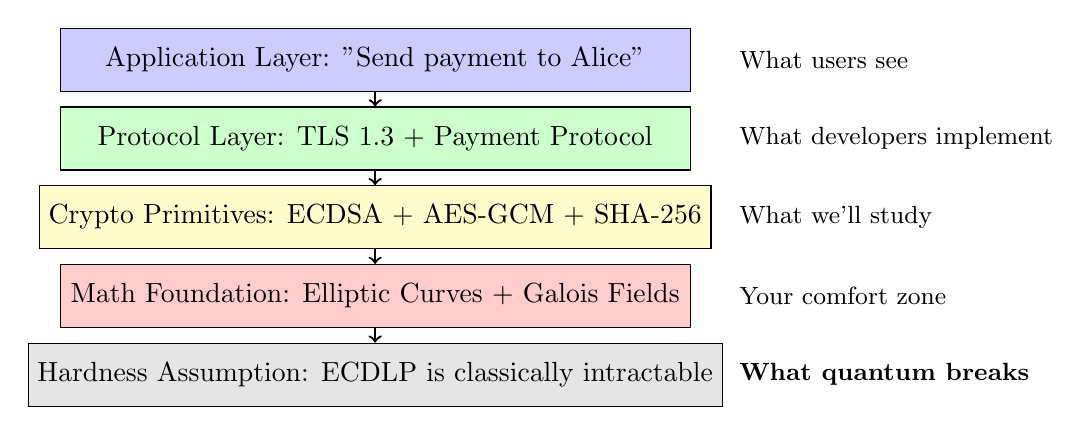
\begin{tikzpicture}[
    box/.style={rectangle, draw, minimum width=8cm, minimum height=0.8cm},
    arrow/.style={->, thick}
]
    % Stack layers
    \node[box, fill=blue!20] (app) at (0,4) {Application Layer: "Send payment to Alice"};
    \node[box, fill=green!20] (proto) at (0,3) {Protocol Layer: TLS 1.3 + Payment Protocol};
    \node[box, fill=yellow!20] (crypto) at (0,2) {Crypto Primitives: ECDSA + AES-GCM + SHA-256};
    \node[box, fill=red!20] (math) at (0,1) {Math Foundation: Elliptic Curves + Galois Fields};
    \node[box, fill=gray!20] (hard) at (0,0) {Hardness Assumption: ECDLP is classically intractable};
    
    % Arrows
    \draw[arrow] (app) -- (proto);
    \draw[arrow] (proto) -- (crypto);
    \draw[arrow] (crypto) -- (math);
    \draw[arrow] (math) -- (hard);
    
    % Side annotations
    \node[align=left, anchor=west] at (4.5,4) {\small What users see};
    \node[align=left, anchor=west] at (4.5,3) {\small What developers implement};
    \node[align=left, anchor=west] at (4.5,2) {\small What we'll study};
    \node[align=left, anchor=west] at (4.5,1) {\small Your comfort zone};
    \node[align=left, anchor=west] at (4.5,0) {\small \textbf{What quantum breaks}};
\end{tikzpicture}
\caption{The cryptographic stack: From user action to mathematical foundation}
\end{figure}

The beautiful complexity extends beyond the obvious applications. Cryptography secures:
\begin{itemize}
    \item \textbf{Your car:} Keyless entry uses rolling codes with AES encryption
    \item \textbf{Your passport:} Contains a cryptographic chip performing challenge-response authentication
    \item \textbf{Your credit card:} EMV chips perform dynamic signature generation for each transaction
    \item \textbf{Your phone's SIM:} Authenticates to cell towers using the MILENAGE algorithm
    \item \textbf{Your smart home:} IoT devices use DTLS (Datagram TLS) for secure communication
    \item \textbf{Software updates:} Every app update is cryptographically signed to prevent tampering
\end{itemize}

\begin{example}[The Cryptographic Cascade]
Let's trace a simple action---unlocking your phone with your fingerprint:
\begin{enumerate}
    \item Fingerprint sensor captures biometric data
    \item Data is hashed using SHA-256 (not stored in plain form)
    \item Hash is compared using a secure enclave processor
    \item Upon match, the enclave releases an AES-256 key
    \item This key decrypts your phone's file system keys
    \item Those keys decrypt your actual data
\end{enumerate}
Five cryptographic operations just to unlock your phone!
\end{example}

The infrastructure is so pervasive that its sudden failure would be catastrophic. If all cryptography stopped working instantly:
\begin{itemize}
    \item All e-commerce would halt (no secure payments)
    \item Email would become postcards (no privacy)
    \item Software couldn't be trusted (no signatures)
    \item Digital identity would collapse (no authentication)
    \item Classified information would be exposed (no confidentiality)
\end{itemize}

This is why the quantum threat matters. We're not protecting some abstract mathematical constructs---we're protecting the fundamental trust layer of human civilization in the 21st century.

\begin{remark}[For the skeptical]
You might think: "Surely not \emph{everything} uses cryptography." Try this experiment: Use Wireshark to monitor your network traffic for 60 seconds while doing nothing. You'll see dozens of encrypted connections---background app updates, cloud syncs, telemetry data, keepalive packets. The invisible infrastructure never sleeps.
\end{remark}

In the next sections, we'll dissect this infrastructure piece by piece, understanding not just what each component does, but why it's vulnerable to quantum attack and how we can rebuild it to be quantum-resistant.

\subsubsection{The Three Pillars of Cryptography}

Most people think cryptography equals secrecy---hiding messages from prying eyes. This mental model is dangerously incomplete. Modern cryptography rests on three equally critical pillars, and the failure of any one can be catastrophic.

\begin{definition}[The Cryptographic Triad]
Complete cryptographic security requires:
\begin{enumerate}
    \item \textbf{Confidentiality:} Only authorized parties can read the data
    \item \textbf{Integrity:} Any tampering with data is detectable  
    \item \textbf{Authentication:} You can verify who you're communicating with
\end{enumerate}
\end{definition}

Let's see why each pillar is essential through real-world failures:

\paragraph{Pillar 1: Confidentiality (Encryption)}

This is what most people think of as "cryptography"---transforming plaintext into ciphertext that only authorized parties can decrypt.

\begin{itemize}
    \item \textbf{Primitives:} AES (symmetric), RSA encryption (asymmetric), ElGamal
    \item \textbf{Purpose:} Prevent unauthorized reading of data
    \item \textbf{Without it:} Every message is a postcard, readable by anyone who intercepts it
\end{itemize}

\begin{example}[Confidentiality Failure]
In 2013, Edward Snowden revealed that the NSA was collecting unencrypted data from Google's internal networks. Between data centers, Google relied on physical security rather than encryption. Result: Massive confidentiality breach despite secure facilities.
\end{example}

\paragraph{Pillar 2: Integrity (Hash Functions and MACs)}

Integrity ensures that any modification to data is detectable. This is \emph{not} about preventing modification---it's about detecting it.

\begin{itemize}
    \item \textbf{Primitives:} SHA-256 (hash), HMAC (keyed hash), GHASH (in AES-GCM)
    \item \textbf{Purpose:} Detect any bit flip, insertion, deletion, or reordering
    \item \textbf{Without it:} Attackers can modify messages undetected
\end{itemize}

\begin{example}[Integrity Failure]
In 2008, researchers demonstrated collision attacks on MD5 certificates. They created a rogue Certificate Authority certificate that had the same hash as a legitimate website certificate. This allowed them to impersonate \emph{any} website because the integrity check (MD5) was broken.
\end{example}

\paragraph{Pillar 3: Authentication (Digital Signatures)}

Authentication proves the identity of the sender and is provided by digital signatures---the digital equivalent of a handwritten signature but unforgeable.

\begin{itemize}
    \item \textbf{Primitives:} RSA signatures, ECDSA, EdDSA
    \item \textbf{Purpose:} Prove who sent a message and that they approve its contents
    \item \textbf{Without it:} Anyone can impersonate anyone else
\end{itemize}

\begin{example}[Authentication Failure]
In 2011, DigiNotar, a Dutch Certificate Authority, was compromised. Attackers issued fraudulent certificates for major domains including *.google.com. Without proper authentication, users' browsers trusted fake websites. The company went bankrupt within months, and the Dutch government fell into crisis as DigiNotar secured government sites.
\end{example}

\paragraph{The Interdependence of the Pillars}

Here's the critical insight: \textbf{these pillars are not independent}. Encryption without authentication is like having a secure phone line to a stranger---you don't know who you're talking to. Authentication without encryption means everyone can verify your signature but also read your messages.

\begin{figure}[h]
\centering
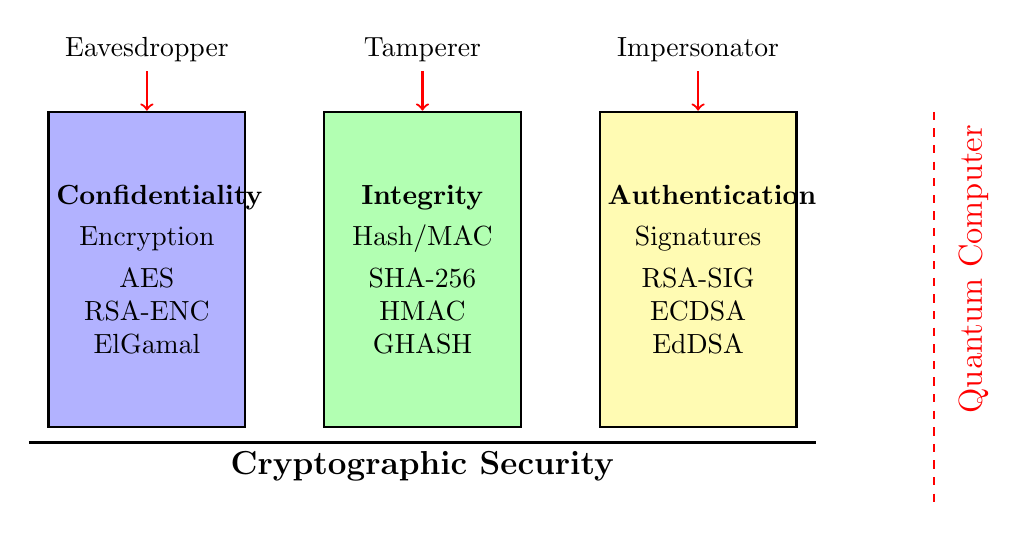
\begin{tikzpicture}[
    pillar/.style={rectangle, draw, thick, minimum width=2.5cm, minimum height=4cm},
    label/.style={text width=2.3cm, align=center},
    attack/.style={->, thick, red}
]
    % Three pillars
    \node[pillar, fill=blue!30] (conf) at (0,0) {};
    \node[label] at (0,0) {\textbf{Confidentiality}\\[0.3em]Encryption\\[0.3em]AES\\RSA-ENC\\ElGamal};
    
    \node[pillar, fill=green!30] (inte) at (3.5,0) {};
    \node[label] at (3.5,0) {\textbf{Integrity}\\[0.3em]Hash/MAC\\[0.3em]SHA-256\\HMAC\\GHASH};
    
    \node[pillar, fill=yellow!30] (auth) at (7,0) {};
    \node[label] at (7,0) {\textbf{Authentication}\\[0.3em]Signatures\\[0.3em]RSA-SIG\\ECDSA\\EdDSA};
    
    % Platform
    \draw[thick] (-1.5,-2.2) -- (8.5,-2.2);
    \node at (3.5,-2.5) {\large\textbf{Cryptographic Security}};
    
    % Attacks
    \node[above=0.5cm of conf] (attacker1) {Eavesdropper};
    \draw[attack] (attacker1) -- (conf);
    
    \node[above=0.5cm of inte] (attacker2) {Tamperer};
    \draw[attack] (attacker2) -- (inte);
    
    \node[above=0.5cm of auth] (attacker3) {Impersonator};
    \draw[attack] (attacker3) -- (auth);
    
    % Quantum threat
    \draw[thick, red, dashed] (10,2) -- (10,-3);
    \node[rotate=90, red] at (10.5,0) {\large Quantum Computer};
\end{tikzpicture}
\caption{The three pillars of cryptography and their attackers}
\end{figure}

\paragraph{Real Protocol Example: Secure Email}

Let's see how all three pillars work together in PGP/GPG email:

\begin{enumerate}
    \item \textbf{Authentication:} Alice signs her email with her private key
    \item \textbf{Integrity:} The signature includes a hash of the message
    \item \textbf{Confidentiality:} The signed message is encrypted with Bob's public key
    \item Bob receives the encrypted package and:
        \begin{itemize}
            \item Decrypts with his private key (confidentiality)
            \item Verifies Alice's signature (authentication)
            \item Checks the hash matches (integrity)
        \end{itemize}
\end{enumerate}

Remove any step and security collapses:
\begin{itemize}
    \item No encryption? Everyone reads Alice's mail
    \item No signature? Eve can send mail claiming to be Alice  
    \item No integrity check? Mallory can modify the message in transit
\end{itemize}

\paragraph{The Quantum Threat to All Three Pillars}

Here's what makes quantum computers so devastating: they don't just threaten one pillar---they demolish two completely and weaken the third:

\begin{itemize}
    \item \textbf{Confidentiality:} Shor's algorithm breaks RSA encryption, ElGamal, and ECC
    \item \textbf{Authentication:} The same algorithm breaks RSA signatures, ECDSA, and DSA
    \item \textbf{Integrity:} Grover's algorithm gives quadratic speedup for finding hash collisions
\end{itemize}

This is why post-quantum cryptography must address all three pillars. It's not enough to have quantum-resistant encryption if signatures remain vulnerable---the entire security architecture would still collapse.

\begin{remark}[A Common Misconception]
Students often ask: "Why not just use AES for everything? It's quantum-resistant!" Because AES (symmetric encryption) only provides confidentiality, and only if you already share a key. It cannot provide authentication (no public/private key pairs) and provides integrity only in special modes like GCM. The three pillars require different mathematical structures.
\end{remark}

Understanding these three pillars is crucial for the rest of our journey. Every cryptographic protocol we examine will use all three, and every quantum threat we discuss will target one or more of these fundamental security properties.


\subsubsection{The Two-Key Revolution}

Before 1976, all cryptography faced a fundamental paradox: to communicate securely, you first had to communicate securely. This circular dependency meant that every encrypted communication required a prior secure exchange of secret keys---a logistical nightmare that limited cryptography to governments, militaries, and large corporations with trusted courier networks.

\paragraph{The Pre-Digital Key Distribution Problem}

Consider the absurd logistics of symmetric-key cryptography at scale:

\begin{example}[The Key Distribution Nightmare]
Imagine 1,000 people wanting to communicate securely with each other:
\begin{itemize}
    \item Each pair needs a unique shared key: $\binom{1000}{2} = 499,500$ keys total
    \item Each person must securely store 999 keys
    \item Adding one new person requires distributing 1,000 new keys
    \item Key compromise affects only one communication pair (good), but requires physical key redistribution (bad)
\end{itemize}
\end{example}

Historical solutions were expensive and limited:
\begin{itemize}
    \item \textbf{Diplomatic bags:} Physical couriers with armed protection
    \item \textbf{Code books:} Pre-distributed keys (vulnerable if captured)
    \item \textbf{One-time pads:} Perfect security but requires key length = message length
    \item \textbf{Key distribution centers:} Single point of failure and trust
\end{itemize}

The Internet was emerging in the 1970s, but secure communication seemed impossible. How could strangers establish secure channels without meeting? How could e-commerce exist if every customer needed pre-shared keys with every merchant?

\paragraph{The "Impossible" Made Possible}

In 1976, Whitfield Diffie and Martin Hellman published "New Directions in Cryptography," solving what experts considered impossible. Their insight was profound yet simple: \textbf{separate the key into two parts with different capabilities}.

\begin{quote}
"We stand today on the brink of a revolution in cryptography. The development of cheap digital hardware has freed it from the design limitations of mechanical computing and brought the cost of high-grade cryptographic devices down to where they can be used in such commercial applications as remote cash dispensers and computer terminals." ---Diffie \& Hellman, 1976
\end{quote}

They were spectacularly right. But even they underestimated the impact---they thought cryptography would be important for "remote cash dispensers," not that it would underpin all human digital interaction.

\paragraph{The Mathematical Magic: One-Way Functions with Trapdoors}

The key insight is that certain mathematical operations are easy in one direction but hard to reverse---unless you have special information (the "trapdoor").

\begin{definition}[One-Way Trapdoor Function]
A function $f: X \to Y$ where:
\begin{enumerate}
    \item \textbf{Easy forward:} Given $x$, computing $f(x)$ is efficient
    \item \textbf{Hard backward:} Given $y$, finding $x$ where $f(x) = y$ is computationally infeasible
    \item \textbf{Trapdoor:} With special information $t$, finding $x$ from $y$ becomes efficient
\end{enumerate}
\end{definition}

\begin{figure}[h]
\centering
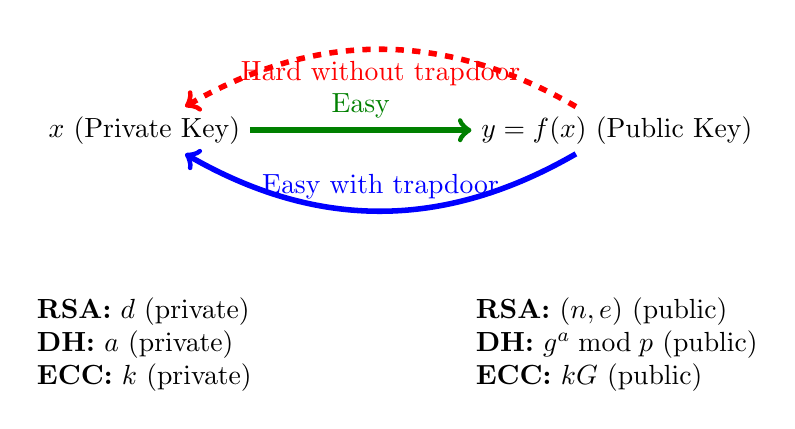
\begin{tikzpicture}[
    arrow/.style={->, thick},
    node distance=4cm
]
    % Forward direction
    \node (x) at (0,0) {$x$ (Private Key)};
    \node (y) at (6,0) {$y = f(x)$ (Public Key)};
    \draw[arrow, green!50!black, line width=2pt] (x) -- node[above] {Easy} (y);
    
    % Backward without trapdoor
    \draw[arrow, red, line width=2pt, dashed] (y) to[bend right=30] node[below] {Hard without trapdoor} (x);
    
    % Backward with trapdoor
    \draw[arrow, blue, line width=2pt] (y) to[bend left=30] node[above] {Easy with trapdoor} (x);
    
    % Examples
    \node[align=left, anchor=north] at (0,-2) {
        \textbf{RSA:} $d$ (private)\\
        \textbf{DH:} $a$ (private)\\
        \textbf{ECC:} $k$ (private)
    };
    
    \node[align=left, anchor=north] at (6,-2) {
        \textbf{RSA:} $(n,e)$ (public)\\
        \textbf{DH:} $g^a \bmod p$ (public)\\
        \textbf{ECC:} $kG$ (public)
    };
\end{tikzpicture}
\caption{The one-way trapdoor principle enabling public key cryptography}
\end{figure}

\paragraph{The Diffie-Hellman Key Exchange: The First Miracle}

The first public key protocol wasn't encryption---it was key agreement. Two strangers can establish a shared secret over an insecure channel:

\begin{algorithm}
\caption{Diffie-Hellman Key Exchange}
\textbf{Public Parameters:} Prime $p$, generator $g$\\
\textbf{Alice:}
\begin{enumerate}
    \item Choose secret $a \in \{2, ..., p-2\}$
    \item Compute $A = g^a \bmod p$
    \item Send $A$ to Bob
\end{enumerate}
\textbf{Bob:}
\begin{enumerate}
    \item Choose secret $b \in \{2, ..., p-2\}$
    \item Compute $B = g^b \bmod p$
    \item Send $B$ to Alice
\end{enumerate}
\textbf{Shared Secret:}
\begin{itemize}
    \item Alice computes: $K = B^a = g^{ab} \bmod p$
    \item Bob computes: $K = A^b = g^{ab} \bmod p$
\end{itemize}
\end{algorithm}

The eavesdropper sees $g$, $p$, $g^a$, and $g^b$ but cannot compute $g^{ab}$ without solving the discrete logarithm problem!

\paragraph{Symmetric vs Asymmetric: A Perfect Partnership}

The revolution created two complementary cryptographic worlds:

\begin{table}[h]
\centering
\begin{tabularx}{\textwidth}{|l|X|X|}
\hline
\textbf{Property} & \textbf{Symmetric Cryptography} & \textbf{Asymmetric Cryptography} \\
\hline
\textbf{Keys} & Single shared secret & Public/private key pair \\
\textbf{Speed} & Very fast (Gbps) & Slow (Mbps) \\
\textbf{Key size} & Small (128-256 bits) & Large (2048-4096 bits) \\
\textbf{Use case} & Bulk data encryption & Key exchange, signatures \\
\textbf{Examples} & AES, ChaCha20 & RSA, ECDH, ECDSA \\
\textbf{Quantum threat} & Grover (manageable) & Shor (catastrophic) \\
\hline
\end{tabularx}
\caption{Complementary strengths of symmetric and asymmetric cryptography}
\end{table}

This led to a beautiful division of labor:
\begin{itemize}
    \item \textbf{Asymmetric:} Establish initial trust and exchange keys
    \item \textbf{Symmetric:} Encrypt actual data efficiently
\end{itemize}

\paragraph{The Hybrid Approach: Best of Both Worlds}

Modern protocols universally use hybrid cryptography. Here's how TLS 1.3 works:

\begin{enumerate}
    \item \textbf{Authentication:} Server proves identity with certificate (digital signature)
    \item \textbf{Key Exchange:} ECDHE establishes shared secret (asymmetric)
    \item \textbf{Key Derivation:} Shared secret generates multiple symmetric keys
    \item \textbf{Bulk Encryption:} All data encrypted with AES-GCM (symmetric)
\end{enumerate}

\begin{lstlisting}[language=Python, caption=Simplified Hybrid Encryption]
def hybrid_encrypt(message, recipient_public_key):
    # Generate ephemeral symmetric key
    symmetric_key = generate_random_key(256)  # 256 bits
    
    # Encrypt message with fast symmetric crypto
    ciphertext = AES_encrypt(message, symmetric_key)
    
    # Encrypt symmetric key with recipient's public key
    encrypted_key = RSA_encrypt(symmetric_key, recipient_public_key)
    
    return (encrypted_key, ciphertext)

def hybrid_decrypt(encrypted_key, ciphertext, private_key):
    # Decrypt symmetric key with private key
    symmetric_key = RSA_decrypt(encrypted_key, private_key)
    
    # Decrypt message with symmetric key
    message = AES_decrypt(ciphertext, symmetric_key)
    
    return message
\end{lstlisting}

This hybrid approach is so fundamental that breaking asymmetric crypto breaks everything, even though symmetric crypto does the actual encryption!

\paragraph{Why This Revolution is Quantum-Vulnerable}

The tragic irony is that the mathematical structures enabling public key cryptography---discrete logarithms and factoring---have hidden periodic structures that quantum computers exploit:

\begin{itemize}
    \item \textbf{Factoring (RSA):} Finding $p,q$ from $n=pq$ reduces to period-finding
    \item \textbf{Discrete Log (DH, DSA, ECDSA):} Finding $x$ from $g^x$ also reduces to period-finding
    \item \textbf{Shor's Algorithm:} Quantum Fourier Transform finds periods exponentially fast
\end{itemize}

This means the entire public key revolution---forty years of deployed infrastructure---collapses against quantum computers. We don't go back to symmetric-only cryptography (that would be impossible at Internet scale). Instead, we must find new mathematical one-way trapdoor functions that resist quantum attack.

\begin{remark}[Historical Irony]
The NSA knew about public key cryptography before 1976 (classified as "non-secret encryption"), but didn't pursue it because they thought key distribution was a solved problem for government use. Diffie and Hellman, outsiders to the cryptographic establishment, revolutionized the field precisely because they saw the civilian need for scalable key distribution. Today's post-quantum transition similarly requires thinking beyond established patterns.
\end{remark}

The two-key revolution made the Internet possible. Every secure connection, digital signature, and cryptocurrency transaction depends on the separation of public and private keys. As we'll see, post-quantum cryptography must preserve this revolutionary capability while replacing its vulnerable mathematical foundations.

\subsubsection{Public Key Infrastructure (PKI)}

Public key cryptography solved key distribution, but created a new problem: how do you know a public key actually belongs to who claims to own it? If you receive a public key claiming to be "Bank of America," how can you verify it's genuine? Without solving this authentication problem, attackers could simply publish their own keys under any name. The solution---Public Key Infrastructure---has become the most successful distributed system in human history, though most people have never heard of it.

\paragraph{The Authentication Problem at Scale}

Consider the challenge: billions of users need to verify the authenticity of millions of websites, without any prior relationship. The naive solutions fail immediately:

\begin{itemize}
    \item \textbf{Manual verification:} "Call the bank to verify their key" ---impossible at scale
    \item \textbf{Central directory:} Single point of failure, massive target
    \item \textbf{Web of trust:} Works for small communities, fails at Internet scale
    \item \textbf{Trust on first use:} Vulnerable to initial impersonation
\end{itemize}

\paragraph{The Elegant Solution: Hierarchical Trust}

PKI solves this through a hierarchy of trust, similar to how government IDs work. You trust your passport because it's issued by your government; you trust a website's certificate because it's signed by a Certificate Authority (CA).

\begin{figure}[h]
\centering
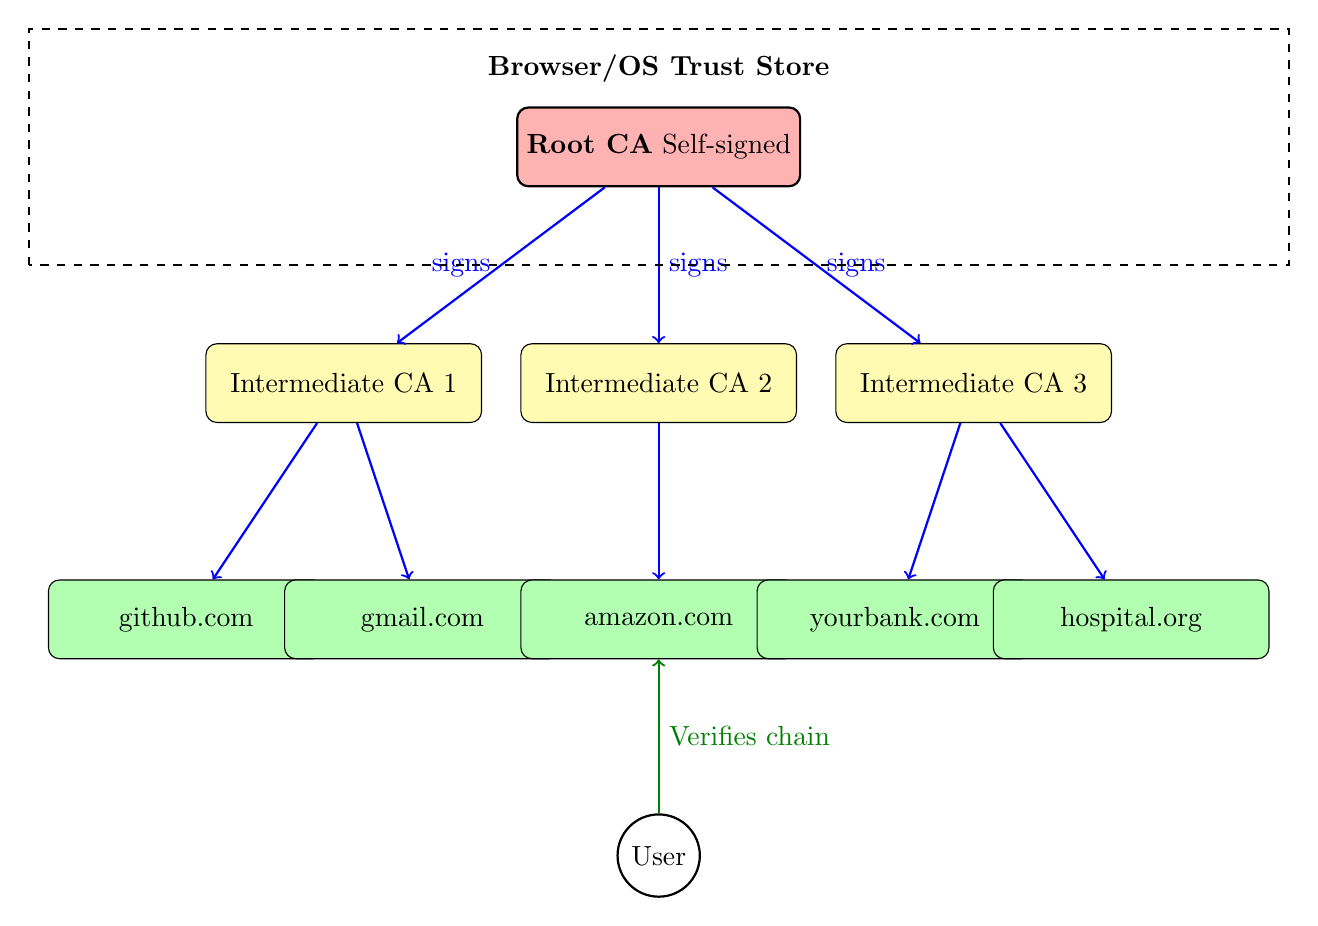
\begin{tikzpicture}[
    cert/.style={rectangle, draw, rounded corners, minimum width=3.5cm, minimum height=1cm},
    arrow/.style={->, thick},
    sig/.style={->, thick, blue}
]
    % Root CA
    \node[cert, fill=red!30, thick] (root) at (0,6) {\textbf{Root CA} Self-signed};
    
    % Intermediate CAs
    \node[cert, fill=yellow!30] (int1) at (-4,3) {Intermediate CA 1};
    \node[cert, fill=yellow!30] (int2) at (0,3) {Intermediate CA 2};
    \node[cert, fill=yellow!30] (int3) at (4,3) {Intermediate CA 3};
    
    % End entities
    \node[cert, fill=green!30] (ee1) at (-6,0) {github.com};
    \node[cert, fill=green!30] (ee2) at (-3,0) {gmail.com};
    \node[cert, fill=green!30] (ee3) at (0,0) {amazon.com};
    \node[cert, fill=green!30] (ee4) at (3,0) {yourbank.com};
    \node[cert, fill=green!30] (ee5) at (6,0) {hospital.org};
    
    % Signatures
    \draw[sig] (root) -- node[left] {signs} (int1);
    \draw[sig] (root) -- node[right] {signs} (int2);
    \draw[sig] (root) -- node[right] {signs} (int3);
    
    \draw[sig] (int1) -- (ee1);
    \draw[sig] (int1) -- (ee2);
    \draw[sig] (int2) -- (ee3);
    \draw[sig] (int3) -- (ee4);
    \draw[sig] (int3) -- (ee5);
    
    % Trust store
    \draw[dashed, thick] (-8,4.5) rectangle (8,7.5);
    \node at (0,7) {\textbf{Browser/OS Trust Store}};
    
    % User
    \node[circle, draw, thick] (user) at (0,-3) {User};
    \draw[arrow, green!50!black] (user) -- node[right] {Verifies chain} (ee3);
\end{tikzpicture}
\caption{PKI hierarchy: From root trust to website authentication}
\end{figure}

\paragraph{Certificate Anatomy}

Let's examine a real certificate to understand what's inside:

\begin{lstlisting}[language=bash, caption=Examining a Real Certificate]
$ openssl s_client -connect github.com:443 -showcerts | \
  openssl x509 -text -noout

Certificate:
    Data:
        Version: 3 (0x2)
        Serial Number:
            0c:1f:cb:18:45:0f:7f:c0:1a:8f:7e:f6:7b:6d:69:51
        Signature Algorithm: sha256WithRSAEncryption
        Issuer: C=US, O=DigiCert Inc, CN=DigiCert TLS RSA SHA256 2020 CA1
        Validity
            Not Before: Mar 15 00:00:00 2024 GMT
            Not After : Mar 15 23:59:59 2025 GMT
        Subject: C=US, ST=California, L=San Francisco, O=GitHub, Inc., 
                 CN=github.com
        Subject Public Key Info:
            Public Key Algorithm: rsaEncryption
                RSA Public-Key: (2048 bit)
                Modulus:
                    00:b1:c3:b3:da:c7:3f:3e:...
        X509v3 extensions:
            X509v3 Subject Alternative Name: 
                DNS:github.com, DNS:*.github.com
            X509v3 Key Usage: critical
                Digital Signature, Key Encipherment
    Signature Algorithm: sha256WithRSAEncryption
         65:f3:97:00:de:3d:8e:42:...
\end{lstlisting}

Each certificate contains:
\begin{itemize}
    \item \textbf{Subject:} Who this certificate identifies
    \item \textbf{Issuer:} Who vouches for this identity
    \item \textbf{Public key:} The actual cryptographic key
    \item \textbf{Validity period:} When the certificate expires
    \item \textbf{Digital signature:} Issuer's cryptographic proof
\end{itemize}

\paragraph{Certificate Chain Validation}

When you connect to a website, your browser performs a complex validation:

\begin{algorithm}
\caption{Certificate Chain Validation}
\textbf{Input:} Server certificate chain $[C_0, C_1, ..., C_n]$\\
\textbf{Output:} Valid or Invalid
\begin{enumerate}
    \item Verify $C_0$ (server cert) matches requested domain
    \item For each certificate $C_i$ in chain:
        \begin{enumerate}
            \item Check current time within validity period
            \item Verify signature: $C_{i+1}$ signed $C_i$
            \item Check $C_i$ not revoked (OCSP/CRL check)
            \item Verify key usage permits operation
        \end{enumerate}
    \item Verify $C_n$ (root) is in trust store
    \item Verify chain length $\leq$ maximum (typically 5)
\end{enumerate}
\end{algorithm}

\paragraph{The Astounding Scale of Success}

PKI operates at a scale that's difficult to comprehend:

\begin{itemize}
    \item \textbf{4+ billion users} rely on PKI daily
    \item \textbf{200+ million certificates} currently active
    \item \textbf{100+ root CAs} in typical trust stores
    \item \textbf{10+ billion certificate validations} performed daily
    \item \textbf{99.999\%+ reliability} across the entire Internet
\end{itemize}

\begin{table}[h]
\centering
\begin{tabular}{|l|r|r|}
\hline
\textbf{Major CA} & \textbf{Certificates Issued} & \textbf{Market Share} \\
\hline
Let's Encrypt & 400+ million & 40\% \\
DigiCert & 50+ million & 15\% \\
Sectigo & 100+ million & 20\% \\
GlobalSign & 25+ million & 5\% \\
Others & 100+ million & 20\% \\
\hline
\end{tabular}
\caption{The certificate authority ecosystem (2024 data)}
\end{table}

\paragraph{When PKI Fails: Catastrophic Consequences}

The few PKI failures demonstrate its critical importance:

\begin{example}[DigiNotar Collapse (2011)]
\begin{itemize}
    \item Iranian hackers compromised Dutch CA DigiNotar
    \item Issued fraudulent certificates for *.google.com
    \item Used for man-in-the-middle attacks against Iranian citizens
    \item DigiNotar bankrupt within weeks
    \item Dutch government fell into crisis (DigiNotar secured government sites)
    \item Led to certificate pinning and Certificate Transparency
\end{itemize}
\end{example}

\begin{example}[Symantec CA Distrust (2017)]
\begin{itemize}
    \item Google discovered Symantec improperly issued 30,000+ certificates
    \item Chrome gradually distrusted all Symantec certificates
    \item Affected millions of websites
    \item Symantec sold CA business to DigiCert
    \item Largest CA migration in Internet history
\end{itemize}
\end{example}

\paragraph{The Invisible Success Story}

PKI's success is measured by what doesn't happen:
\begin{itemize}
    \item You don't think about verifying website identity
    \item You don't manually exchange keys with every service
    \item You don't worry about impostor websites (with valid HTTPS)
    \item Software updates install without malware injection
    \item Email servers authenticate automatically
\end{itemize}

This invisibility is PKI's greatest achievement and biggest vulnerability---users don't understand what they depend on.

\paragraph{Why PKI is Quantum-Vulnerable}

The entire PKI hierarchy depends on digital signatures:
\begin{itemize}
    \item Root certificates: Self-signed with RSA or ECDSA
    \item Intermediate certificates: Signed by roots
    \item End-entity certificates: Signed by intermediates
    \item Certificate revocation lists: Signed by CAs
    \item OCSP responses: Signed by CA delegates
\end{itemize}

When quantum computers can forge signatures:
\begin{itemize}
    \item Attackers can create fake certificates for any domain
    \item Can sign malware as Microsoft, Apple, or Google
    \item Can impersonate any certificate authority
    \item Trust hierarchy collapses completely
\end{itemize}

\begin{remark}[The Migration Challenge]
Replacing PKI with post-quantum signatures isn't just a technical challenge---it's a coordination problem. Every browser, operating system, server, and IoT device must update. A single widely-used system that doesn't update becomes a weakness. This is why PKI migration to PQC must start now, even though the quantum threat is years away.
\end{remark}

\begin{example}[Certificate Size Impact]
Current certificate chain (RSA-2048): ~4 KB\\
Post-quantum chain (Dilithium3): ~15 KB\\
Impact: 3.75× bandwidth increase for every HTTPS connection\\
For Google, serving 100 billion requests/day: 1.1 PB additional traffic daily
\end{example}

PKI represents humanity's largest successful distributed trust system. Its invisible operation enables the entire digital economy. The quantum threat to PKI isn't just about mathematics---it's about preserving the foundation of digital trust that billions depend on without even knowing it exists.

\subsubsection{Case Study: TLS Protocol}

Every time you see that padlock icon in your browser, one of the most sophisticated cryptographic protocols ever designed has just executed. Transport Layer Security (TLS) seamlessly combines every concept we've discussed---digital signatures, key exchange, certificates, symmetric encryption---into a protocol that secures trillions of connections daily. Let's dissect what actually happens when you visit an HTTPS website.

\paragraph{The Millisecond Miracle}

In approximately 400 milliseconds, TLS accomplishes what once required diplomatic pouches and armed couriers:

\begin{itemize}
    \item \textbf{Authenticates} the server (and optionally client)
    \item \textbf{Negotiates} cryptographic parameters
    \item \textbf{Establishes} shared secrets with perfect forward secrecy
    \item \textbf{Derives} multiple encryption keys
    \item \textbf{Begins} encrypted communication
\end{itemize}

All while defending against dozens of possible attacks and maintaining backward compatibility with billions of devices.

\paragraph{The TLS 1.3 Handshake: A Cryptographic Symphony}

Let's trace through an actual TLS 1.3 connection:

\begin{figure}[h]
\centering
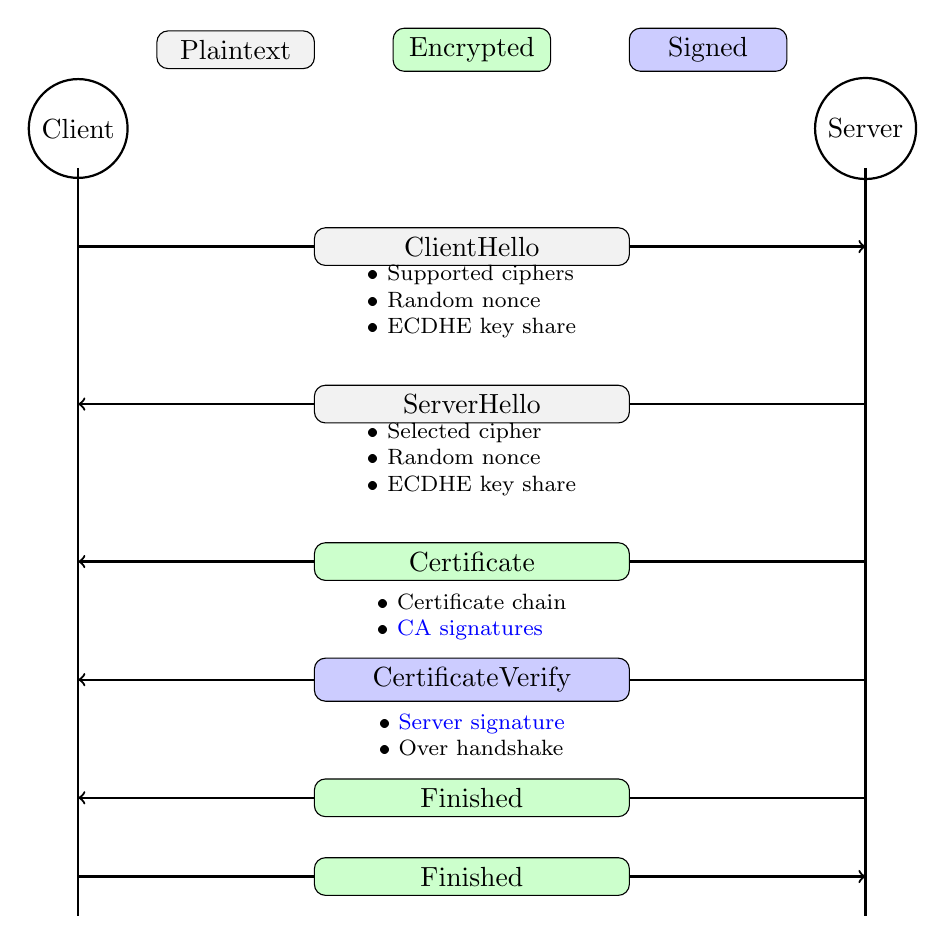
\begin{tikzpicture}[
    packet/.style={rectangle, draw, rounded corners, minimum width=4cm},
    arrow/.style={->, thick},
    encrypt/.style={fill=green!20},
    sign/.style={fill=blue!20},
    plain/.style={fill=gray!10}
]
    % Client and Server
    \node[circle, draw, thick] (client) at (0,0) {Client};
    \node[circle, draw, thick] (server) at (10,0) {Server};
    
    % Time axis
    \draw[thick] (0,-0.5) -- (0,-10);
    \draw[thick] (10,-0.5) -- (10,-10);
    
    % Message flows
    % ClientHello
    \node[packet, plain] (ch) at (5,-1.5) {ClientHello};
    \draw[arrow] (0,-1.5) -- (ch) -- (10,-1.5);
    \node[align=left, font=\footnotesize] at (5,-2.2) {
        • Supported ciphers\\
        • Random nonce\\
        • ECDHE key share
    };
    
    % ServerHello
    \node[packet, plain] (sh) at (5,-3.5) {ServerHello};
    \draw[arrow] (10,-3.5) -- (sh) -- (0,-3.5);
    \node[align=left, font=\footnotesize] at (5,-4.2) {
        • Selected cipher\\
        • Random nonce\\
        • ECDHE key share
    };
    
    % Server Certificate
    \node[packet, encrypt] (cert) at (5,-5.5) {Certificate};
    \draw[arrow] (10,-5.5) -- (cert) -- (0,-5.5);
    \node[align=left, font=\footnotesize] at (5,-6.2) {
        • Certificate chain\\
        • \textcolor{blue}{CA signatures}
    };
    
    % CertificateVerify
    \node[packet, sign] (cv) at (5,-7) {CertificateVerify};
    \draw[arrow] (10,-7) -- (cv) -- (0,-7);
    \node[align=left, font=\footnotesize] at (5,-7.7) {
        • \textcolor{blue}{Server signature}\\
        • Over handshake
    };
    
    % Finished
    \node[packet, encrypt] (fin) at (5,-8.5) {Finished};
    \draw[arrow] (10,-8.5) -- (fin) -- (0,-8.5);
    
    % Client Finished
    \node[packet, encrypt] (cfin) at (5,-9.5) {Finished};
    \draw[arrow] (0,-9.5) -- (cfin) -- (10,-9.5);
    
    % Legend
    \node[packet, plain, minimum width=2cm] at (2,1) {Plaintext};
    \node[packet, encrypt, minimum width=2cm] at (5,1) {Encrypted};
    \node[packet, sign, minimum width=2cm] at (8,1) {Signed};
\end{tikzpicture}
\caption{TLS 1.3 handshake: From first contact to encrypted channel}
\end{figure}

\paragraph{Step-by-Step Cryptographic Operations}

\textbf{Step 1: ClientHello (Client → Server)}
\begin{lstlisting}[language=C, caption=ClientHello Contents]
ClientHello {
    legacy_version: 0x0303,        // Compatibility
    random: [32 random bytes],     // Freshness
    cipher_suites: [              // Supported algorithms
        TLS_AES_128_GCM_SHA256,
        TLS_AES_256_GCM_SHA384,
        TLS_CHACHA20_POLY1305_SHA256
    ],
    extensions: {
        supported_groups: [x25519, secp256r1],  // ECDHE curves
        key_share: {                            // Client's public key
            group: x25519,
            key_exchange: [32-byte public key]
        },
        signature_algorithms: [                 // For certificates
            ecdsa_secp256r1_sha256,
            rsa_pss_rsae_sha256
        ]
    }
}
\end{lstlisting}

The client immediately offers its ECDHE public key, enabling the server to compute the shared secret in its first response.

\textbf{Step 2: ServerHello (Server → Client)}
\begin{itemize}
    \item Server selects mutually supported cipher suite
    \item Provides its ECDHE public key share
    \item Both sides can now compute the shared secret!
\end{itemize}

\textbf{Key Derivation:} Both sides compute:
\begin{align}
\text{ECDHE shared secret} &= \text{ECDH}(\text{client\_private}, \text{server\_public})\\
\text{Handshake Secret} &= \text{HKDF}(\text{shared secret}, \text{transcript hash})\\
\text{Multiple keys} &= \text{HKDF-Expand}(\text{Handshake Secret})
\end{align}

From one shared secret, TLS derives:
\begin{itemize}
    \item client\_handshake\_traffic\_secret
    \item server\_handshake\_traffic\_secret
    \item client\_application\_traffic\_secret
    \item server\_application\_traffic\_secret
    \item resumption\_master\_secret
\end{itemize}

\textbf{Step 3: Server Certificate (Encrypted!)}

Unlike TLS 1.2, the certificate is now encrypted:
\begin{itemize}
    \item Prevents passive observers from seeing which site you're visiting
    \item Certificate chain includes 2-4 certificates
    \item Each certificate contains an RSA or ECDSA public key
    \item Each signed by the next certificate in chain
    \item Root certificate must be in client's trust store
\end{itemize}

\textbf{Step 4: CertificateVerify}

The server proves it owns the private key by signing the handshake:
\begin{lstlisting}[language=C]
signature = Sign(server_private_key, 
                 "TLS 1.3, server CertificateVerify" ||
                 0x20 * 64 ||  // Context string
                 SHA256(ClientHello...ServerCert))
\end{lstlisting}

This signature prevents:
\begin{itemize}
    \item Replay attacks (includes fresh randoms)
    \item Downgrade attacks (covers negotiated parameters)
    \item Certificate substitution (signs exact certificate sent)
\end{itemize}

\textbf{Step 5: Finished Messages}

Both sides send a MAC over the entire handshake:
\begin{align}
\text{finished\_key} &= \text{HKDF-Expand}(\text{traffic\_secret}, "finished")\\
\text{verify\_data} &= \text{HMAC}(\text{finished\_key}, \text{transcript\_hash})
\end{align}

\paragraph{The Resulting Cryptographic Properties}

After these 400 milliseconds, TLS provides:

\begin{enumerate}
    \item \textbf{Server Authentication:} Certificate chain + signature prove server identity
    \item \textbf{Key Exchange:} ECDHE establishes shared secrets
    \item \textbf{Forward Secrecy:} Ephemeral keys mean past sessions stay secure
    \item \textbf{Confidentiality:} AES-GCM encrypts all application data
    \item \textbf{Integrity:} AEAD prevents any tampering
    \item \textbf{Replay Prevention:} Fresh randoms prevent reuse
    \item \textbf{Protocol Negotiation:} Secure agreement on parameters
\end{enumerate}

\paragraph{Performance Engineering}

TLS 1.3 optimizations show how critical performance is:

\begin{itemize}
    \item \textbf{1-RTT handshake:} Full security in one round trip
    \item \textbf{0-RTT resumption:} Repeat connections send data immediately
    \item \textbf{Fewer messages:} Compared to TLS 1.2's 2-RTT handshake
    \item \textbf{Encrypted certificates:} Better privacy without extra cost
\end{itemize}

\begin{table}[h]
\centering
\begin{tabular}{|l|r|r|r|}
\hline
\textbf{Operation} & \textbf{Time (ms)} & \textbf{CPU Cycles} & \textbf{Frequency} \\
\hline
ECDHE key generation & 0.25 & 500,000 & Once \\
ECDHE shared secret & 0.30 & 600,000 & Once \\
Certificate verify (RSA) & 0.05 & 100,000 & Once \\
Certificate sign (RSA) & 2.00 & 4,000,000 & Once \\
AES-GCM setup & 0.01 & 20,000 & Once \\
AES-GCM per KB & 0.002 & 4,000 & Continuous \\
\hline
\textbf{Total handshake} & \textbf{~3ms} & \textbf{~6M cycles} & Per connection \\
\hline
\end{tabular}
\caption{Computational cost of TLS 1.3 operations}
\end{table}

\paragraph{What Makes TLS Remarkable}

TLS succeeds because it:
\begin{itemize}
    \item \textbf{Hides complexity:} Users see only a padlock
    \item \textbf{Adapts constantly:} New versions address emerging threats
    \item \textbf{Scales massively:} Same protocol for IoT devices and supercomputers
    \item \textbf{Maintains compatibility:} Graceful fallback for older systems
    \item \textbf{Prevents diverse attacks:} Defends against dozens of attack types
\end{itemize}

\paragraph{Why Quantum Computers Devastate TLS}

Every single public-key operation in TLS fails against quantum computers:

\begin{itemize}
    \item \textbf{Certificate signatures:} Shor's algorithm forges any certificate
    \item \textbf{ECDHE key exchange:} Quantum computers solve ECDLP
    \item \textbf{CertificateVerify:} Server authentication becomes forgeable
    \item \textbf{RSA key transport:} (TLS 1.2) Completely broken
\end{itemize}

The symmetric operations (AES-GCM, HMAC) survive with larger keys, but without functioning public-key crypto, you can't establish the symmetric keys securely!

\begin{example}[Quantum Attack on TLS]
Attacker with quantum computer:
\begin{enumerate}
    \item Intercepts ClientHello with ECDHE public key
    \item Uses Shor's algorithm to find private key
    \item Computes all session keys
    \item Decrypts entire communication
    \item Can also forge certificates to impersonate any server
\end{enumerate}
Time required: Minutes to hours (vs. universe lifetime classically)
\end{example}

\begin{remark}[The Migration Imperative]
TLS protects approximately:
\begin{itemize}
    \item 5 billion web browsing users
    \item 300 billion daily HTTPS connections
    \item \$4 trillion in annual e-commerce
    \item Every software update and API call
\end{itemize}
Migrating TLS to post-quantum cryptography isn't optional---it's existential for the digital economy.
\end{remark}

This case study shows how modern cryptography weaves together multiple primitives into protocols that seem simple but embody decades of engineering. When we discuss post-quantum replacements, remember: we're not just replacing algorithms, we're preserving this entire intricate dance that happens invisibly billions of times daily.

\subsection{The Computational Hardness Foundation}
\label{sec:hardness}

\subsubsection{The Mathematical Bedrock}

Here's a fact that should terrify you: the entire global digital security infrastructure---every secure message, every digital signature, every cryptocurrency transaction---depends on exactly three mathematical problems. Not three types of problems. Three specific problems. If any efficient algorithm is discovered for these problems, digital security collapses overnight. This mathematical monoculture is both cryptography's greatest success and its greatest vulnerability.

\paragraph{The Narrow Foundation}

Consider the asymmetry: millions of developers implement cryptography, billions of users depend on it, but only three mathematical problems protect everything:

\begin{figure}[h]
\centering
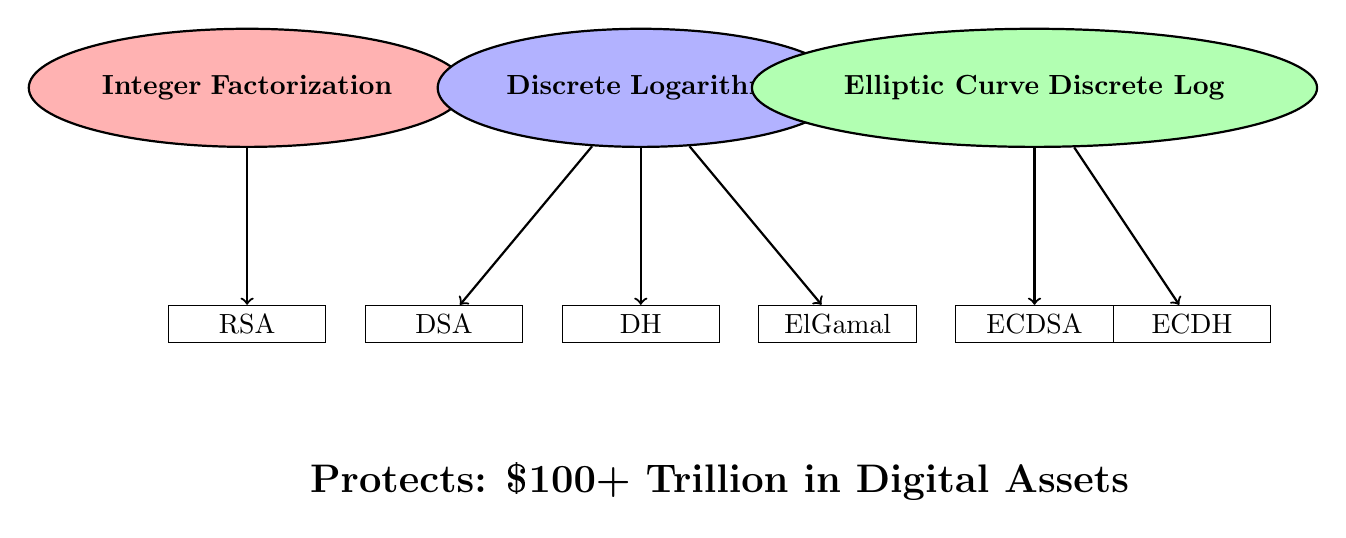
\begin{tikzpicture}[
    problem/.style={ellipse, draw, thick, minimum width=3cm, minimum height=1.5cm},
    algo/.style={rectangle, draw, minimum width=2cm},
    arrow/.style={->, thick}
]
    % The three problems
    \node[problem, fill=red!30] (ifp) at (0,0) {\textbf{Integer} \textbf{Factorization}};
    \node[problem, fill=blue!30] (dlp) at (5,0) {\textbf{Discrete} \textbf{Logarithm}};
    \node[problem, fill=green!30] (ecdlp) at (10,0) {\textbf{Elliptic Curve} \textbf{Discrete Log}};
    
    % Cryptosystems
    \node[algo] (rsa) at (0,-3) {RSA};
    \node[algo] (dsa) at (2.5,-3) {DSA};
    \node[algo] (dh) at (5,-3) {DH};
    \node[algo] (elgamal) at (7.5,-3) {ElGamal};
    \node[algo] (ecdsa) at (10,-3) {ECDSA};
    \node[algo] (ecdh) at (12,-3) {ECDH};
    
    % Connections
    \draw[arrow] (ifp) -- (rsa);
    \draw[arrow] (dlp) -- (dsa);
    \draw[arrow] (dlp) -- (dh);
    \draw[arrow] (dlp) -- (elgamal);
    \draw[arrow] (ecdlp) -- (ecdsa);
    \draw[arrow] (ecdlp) -- (ecdh);
    
    % Usage
    \node at (6,-5) {\Large\textbf{Protects: \$100+ Trillion in Digital Assets}};
\end{tikzpicture}
\caption{The three pillars of mathematical security}
\end{figure}

\paragraph{What Makes a Problem Cryptographically Useful?}

Not every hard mathematical problem can support cryptography. The requirements are stringent:

\begin{definition}[Cryptographically Useful Hard Problem]
A problem suitable for cryptography must have:
\begin{enumerate}
    \item \textbf{Hardness gap:} Easy with secret, hard without
    \item \textbf{Efficient verification:} Solutions checkable in polynomial time
    \item \textbf{Algebraic structure:} Enables operations on encrypted data
    \item \textbf{Scalable hardness:} Difficulty grows smoothly with parameter size
    \item \textbf{Well-studied:} Decades without efficient algorithms
\end{enumerate}
\end{definition}

Thousands of problems in computer science are believed hard (P vs NP contains infinitely many), but only a handful meet all these criteria. Let's examine the three that built the Internet.

\paragraph{Problem 1: The Integer Factorization Problem (IFP)}

\begin{definition}[Integer Factorization Problem]
Given: A composite integer $n = pq$ where $p$ and $q$ are large primes\\
Find: The factors $p$ and $q$
\end{definition}

The beauty lies in the asymmetry:
\begin{itemize}
    \item \textbf{Multiplication:} Given $p = 10^{300} + 357$ and $q = 10^{300} + 577$, computing $n = pq$ takes microseconds
    \item \textbf{Factorization:} Given only $n$, finding $p$ and $q$ takes longer than the universe has existed
\end{itemize}

\begin{example}[Concrete Difficulty Scaling]
\begin{center}
\begin{tabular}{|r|l|l|}
\hline
\textbf{Bits} & \textbf{Example $n$} & \textbf{Factoring Time (Classical)} \\
\hline
20 & 1,048,309 & Microseconds \\
64 & 18,446,744,073,709,551,437 & Seconds \\
128 & 340,282,366,920,938,463,374,875,442,601 & Hours \\
512 & RSA-155 (broken 1999) & 8,000 MIPS-years \\
1024 & RSA-309 & $\sim 10^{12}$ years \\
2048 & Current standard & $\sim 10^{20}$ years \\
\hline
\end{tabular}
\end{center}
\end{example}

Best classical algorithm: General Number Field Sieve
\begin{equation}
\text{Time} = \exp\left(c \cdot (n)^{1/3} \cdot (\log \log n)^{2/3}\right)
\end{equation}
where $c \approx 1.923$. This sub-exponential but super-polynomial growth creates the cryptographic gap.

\paragraph{Problem 2: The Discrete Logarithm Problem (DLP)}

\begin{definition}[Discrete Logarithm Problem]
Given: A group $G$, generator $g \in G$, and element $h \in G$\\
Find: Integer $x$ such that $g^x = h$ in $G$
\end{definition}

In the multiplicative group $\mathbb{Z}_p^*$ (integers modulo prime $p$):
\begin{itemize}
    \item \textbf{Exponentiation:} Given $g = 5$, $x = 76543$, $p = 10^{308} + 129$, computing $h = g^x \bmod p$ is fast
    \item \textbf{Logarithm:} Given $g$, $h$, and $p$, finding $x$ is infeasible
\end{itemize}

The discrete logarithm is the modular arithmetic analog of ordinary logarithms, but dramatically harder:
\begin{align}
\text{Real numbers:} \quad & 2^x = 1024 \implies x = \log_2(1024) = 10 \quad \text{(Easy)}\\
\text{Modular arithmetic:} \quad & 2^x \equiv 1024 \pmod{p} \implies x = ? \quad \text{(Hard)}
\end{align}

\paragraph{Problem 3: The Elliptic Curve Discrete Logarithm Problem (ECDLP)}

\begin{definition}[Elliptic Curve Discrete Logarithm Problem]
Given: Elliptic curve $E$ over finite field, base point $G \in E$, point $P \in E$\\
Find: Integer $k$ such that $kG = P$ (using elliptic curve addition)
\end{definition}

Elliptic curves provide the same discrete logarithm hardness with much smaller numbers:

\begin{example}[Elliptic Curve Efficiency]
\begin{center}
\begin{tabular}{|l|r|r|r|}
\hline
\textbf{Security Level} & \textbf{RSA/DLP} & \textbf{ECC} & \textbf{Ratio} \\
\hline
80 bits & 1,024 bits & 160 bits & 6.4:1 \\
128 bits & 3,072 bits & 256 bits & 12:1 \\
256 bits & 15,360 bits & 512 bits & 30:1 \\
\hline
\end{tabular}
\end{center}
\end{example}

The curve equation (simplified Weierstrass form):
\begin{equation}
y^2 = x^3 + ax + b \pmod{p}
\end{equation}

Point addition uses geometric intuition translated to algebra:
\begin{align}
P + Q &= R \text{ where line through } P,Q \text{ intersects curve at } -R\\
P + P &= 2P \text{ using tangent line at } P
\end{align}

\paragraph{The Deep Connection}

These problems share a hidden connection that explains their cryptographic utility:

\begin{theorem}[Hidden Subgroup Problem]
All three problems reduce to finding hidden subgroups:
\begin{itemize}
    \item \textbf{Factoring:} Find subgroup of $\mathbb{Z}_n^*$ generated by $x \mapsto x^2$
    \item \textbf{DLP:} Find period of $f(a,b) = g^a h^b$
    \item \textbf{ECDLP:} Find period in elliptic curve group
\end{itemize}
\end{theorem}

This connection explains why:
1. Similar classical algorithms work (Pollard $\rho$, index calculus variants)
2. The same quantum algorithm (Shor) breaks all three
3. They provide similar cryptographic functionality

\paragraph{Why These Three Dominated}

Historical and mathematical reasons created this monoculture:

\begin{enumerate}
    \item \textbf{Early discovery:} RSA (1977), DH (1976) came first
    \item \textbf{Patent landscape:} RSA patent expired 2000, allowing widespread use
    \item \textbf{Implementation maturity:} 40+ years of optimization
    \item \textbf{Mathematical elegance:} Clean algebraic structure
    \item \textbf{Efficiency tradeoffs:} Good balance of key size vs. computation
    \item \textbf{Resistance to classical attacks:} No breakthrough despite huge efforts
\end{enumerate}

\paragraph{The Monoculture Risk}

This narrow foundation creates systemic risk:

\begin{itemize}
    \item \textbf{Single point of failure:} One algorithmic breakthrough breaks everything
    \item \textbf{Quantum vulnerability:} All three fall to the same quantum algorithm
    \item \textbf{Implementation similarity:} Side-channel attacks often transfer
    \item \textbf{Limited diversity:} Few backup options if problems fall
\end{itemize}

\begin{remark}[The Search for Problem \#4]
Cryptographers have desperately sought a fourth problem for decades:
\begin{itemize}
    \item Lattice problems (finally successful!)
    \item Knapsack problems (broken in 1980s)
    \item Code-based problems (large keys limited adoption)
    \item Multivariate polynomials (repeated breaks)
    \item Isogenies (SIKE broken in 2022)
\end{itemize}
The difficulty of finding new problems underscores how special these three are.
\end{remark}

\begin{example}[Near Miss: The Knapsack Cryptosystem]
In 1978, Merkle-Hellman proposed using the knapsack problem:
\begin{itemize}
    \item Given: Set of weights $\{a_1, ..., a_n\}$ and sum $S$
    \item Find: Subset summing to exactly $S$
    \item Problem: NP-complete, should be hard!
    \item Reality: Broken by Shamir in 1982 using lattice reduction
    \item Lesson: Not all hard problems make good cryptography
\end{itemize}
\end{example}

This mathematical bedrock supported the entire digital revolution. That it consists of only three problems is both a testament to their power and a warning about our vulnerability. When quantum computers arrive, this narrow foundation becomes a single point of catastrophic failure---motivating the urgent search for quantum-resistant alternatives we'll explore in the remainder of this lecture.

\subsubsection{From Hard Problems to Cryptosystems}

Having a hard mathematical problem is necessary but not sufficient for cryptography. The journey from "factoring is hard" to "RSA is secure" involves subtle constructions, security proofs, and countless implementation details. Many cryptosystems have failed not because their underlying problem was easy, but because the construction was flawed. Understanding this gap is crucial for evaluating post-quantum proposals.

\paragraph{The Reduction Concept: Proving Security}

Cryptographers cannot prove systems are secure in an absolute sense. Instead, they prove security through reductions:

\begin{definition}[Security Reduction]
A security reduction shows: If you can break the cryptosystem with resources $(t, \epsilon)$, then you can solve the underlying hard problem with resources $(t', \epsilon')$ where $t' \approx t$ and $\epsilon' \approx \epsilon$.

Contrapositive: If the problem is hard, the cryptosystem is secure.
\end{definition}

\begin{figure}[h]
\centering
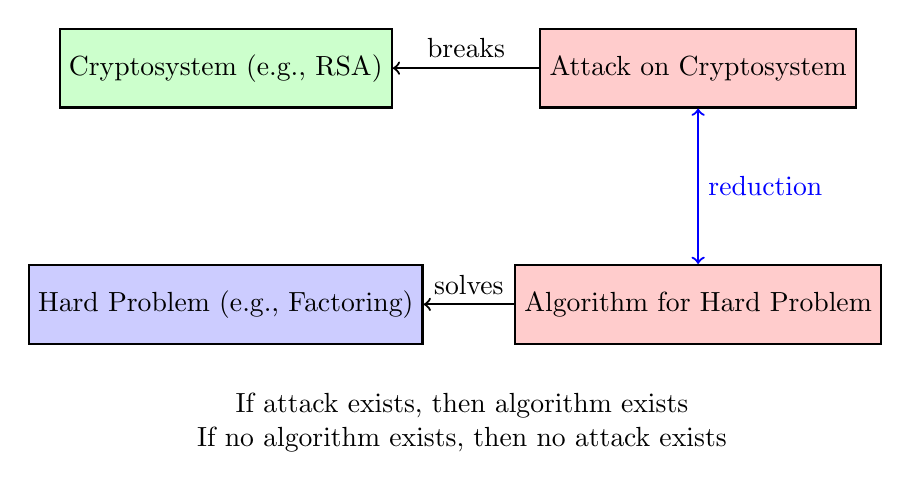
\begin{tikzpicture}[
    box/.style={rectangle, draw, thick, minimum width=3cm, minimum height=1cm},
    arrow/.style={->, thick},
    reduction/.style={<->, thick, blue}
]
    % Top level: Cryptosystem
    \node[box, fill=green!20] (crypto) at (0,3) {Cryptosystem (e.g., RSA)};
    \node[box, fill=red!20] (attack) at (6,3) {Attack on Cryptosystem};
    
    % Bottom level: Hard problem
    \node[box, fill=blue!20] (problem) at (0,0) {Hard Problem (e.g., Factoring)};
    \node[box, fill=red!20] (solution) at (6,0) {Algorithm for Hard Problem};
    
    % Arrows
    \draw[arrow] (attack) -- node[above] {breaks} (crypto);
    \draw[arrow] (solution) -- node[above] {solves} (problem);
    
    % Reduction
    \draw[reduction] (attack) -- node[right] {reduction} (solution);
    
    % Logic
    \node[align=center] at (3,-1.5) {If attack exists, then algorithm exists\\
    If no algorithm exists, then no attack exists};
\end{tikzpicture}
\caption{Security reduction: Cryptosystem security reduces to problem hardness}
\end{figure}

\paragraph{Case Study: From Factoring to RSA}

Let's trace the complete construction of RSA from the factoring assumption:

\textbf{Step 1: The Mathematical Foundation}
\begin{itemize}
    \item Hard problem: Given $n = pq$, find $p$ and $q$
    \item Euler's theorem: For $\gcd(m, n) = 1$: $m^{\phi(n)} \equiv 1 \pmod{n}$
    \item Where $\phi(n) = (p-1)(q-1)$ (Euler's totient function)
\end{itemize}

\textbf{Step 2: The Basic Construction}
\begin{algorithm}
\caption{Textbook RSA Construction}
\begin{algorithmic}
\State \textbf{KeyGen:}
\State \quad Choose large primes $p, q$ (e.g., 1024 bits each)
\State \quad Compute $n = pq$ and $\phi(n) = (p-1)(q-1)$
\State \quad Choose $e$ with $\gcd(e, \phi(n)) = 1$ (often $e = 65537$)
\State \quad Compute $d$ where $ed \equiv 1 \pmod{\phi(n)}$
\State \quad Public key: $(n, e)$; Private key: $d$
\State
\State \textbf{Encrypt}$(m, (n,e))$:
\State \quad Return $c = m^e \bmod n$
\State
\State \textbf{Decrypt}$(c, d)$:
\State \quad Return $m = c^d \bmod n$
\end{algorithmic}
\end{algorithm}

\textbf{Why it works:}
\begin{align}
c^d &= (m^e)^d = m^{ed} \pmod{n}\\
&= m^{1 + k\phi(n)} \text{ for some integer } k\\
&= m \cdot (m^{\phi(n)})^k\\
&= m \cdot 1^k = m \pmod{n}
\end{align}

\paragraph{The Dangerous Gap: Textbook RSA is Insecure!}

The basic construction above is completely insecure in practice:

\begin{example}[Malleability Attack on Textbook RSA]
Given encryption of $m$: $c = m^e \bmod n$
\begin{itemize}
    \item Attacker computes: $c' = c \cdot 2^e = (m \cdot 2)^e \bmod n$
    \item Gets decryption: $m' = 2m$
    \item Recovers: $m = m'/2$
\end{itemize}
Attacker decrypts without knowing $d$!
\end{example}

\begin{example}[Small Message Attack]
If $m < n^{1/e}$, then $m^e < n$, so:
\begin{itemize}
    \item $c = m^e \bmod n = m^e$ (no modular reduction!)
    \item Attacker computes: $m = c^{1/e}$ (ordinary $e$-th root)
\end{itemize}
\end{example}

\paragraph{The Secure Construction: RSA with OAEP}

Real RSA uses Optimal Asymmetric Encryption Padding (OAEP):

\begin{figure}[h]
\centering
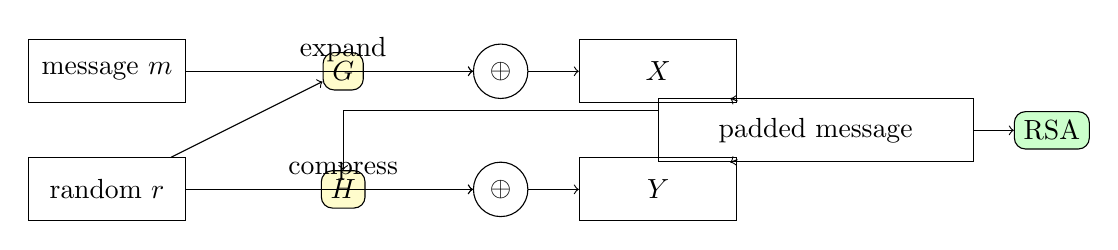
\begin{tikzpicture}[
    box/.style={rectangle, draw, minimum width=2cm, minimum height=0.8cm},
    func/.style={rectangle, draw, rounded corners},
    arrow/.style={->}
]
    % Input message
    \node[box] (m) at (0,3) {message $m$};
    \node[box] (r) at (0,1.5) {random $r$};
    
    % OAEP padding
    \node[func, fill=yellow!20] (g) at (3,3) {$G$};
    \node[func, fill=yellow!20] (h) at (3,1.5) {$H$};
    
    % XOR operations
    \node[circle, draw] (xor1) at (5,3) {$\oplus$};
    \node[circle, draw] (xor2) at (5,1.5) {$\oplus$};
    
    % Output
    \node[box] (x) at (7,3) {$X$};
    \node[box] (y) at (7,1.5) {$Y$};
    
    % Final
    \node[box, minimum width=4cm] (pad) at (9,2.25) {padded message};
    
    % Connections
    \draw[arrow] (m) -- (xor1);
    \draw[arrow] (r) -- (g);
    \draw[arrow] (g) -- (xor1);
    \draw[arrow] (xor1) -- (x);
    
    \draw[arrow] (x) -- +(0,-0.5) -| (h);
    \draw[arrow] (h) -- (xor2);
    \draw[arrow] (r) -- (xor2);
    \draw[arrow] (xor2) -- (y);
    
    \draw[arrow] (x) -- (pad);
    \draw[arrow] (y) -- (pad);
    
    % RSA operation
    \node[func, fill=green!20] (rsa) at (12,2.25) {RSA};
    \draw[arrow] (pad) -- (rsa);
    
    % Labels
    \node[above] at (g) {expand};
    \node[above] at (h) {compress};
\end{tikzpicture}
\caption{RSA-OAEP: Secure padding before encryption}
\end{figure}

OAEP provides:
\begin{itemize}
    \item \textbf{Randomization:} Same message encrypts differently each time
    \item \textbf{All-or-nothing:} Cannot decrypt partially
    \item \textbf{Non-malleability:} Cannot create related ciphertexts
    \item \textbf{Chosen-ciphertext security:} Provably secure in random oracle model
\end{itemize}

\paragraph{Other Constructions from Our Three Problems}

\textbf{Diffie-Hellman Key Exchange:}
\begin{itemize}
    \item Problem: Discrete logarithm in $\mathbb{Z}_p^*$
    \item Construction: Exchange $g^a, g^b$; compute $g^{ab}$
    \item Security: Computing $g^{ab}$ from $g^a, g^b$ is hard (CDH assumption)
    \item Subtlety: Needs authentication to prevent man-in-the-middle
\end{itemize}

\textbf{DSA (Digital Signature Algorithm):}
\begin{itemize}
    \item Problem: Discrete logarithm in subgroup of $\mathbb{Z}_p^*$
    \item Construction: Complex - uses ephemeral keys, modular arithmetic
    \item Security: Forging requires solving discrete log
    \item Subtlety: Reusing ephemeral key reveals private key instantly!
\end{itemize}

\textbf{ECDSA (Elliptic Curve DSA):}
\begin{itemize}
    \item Problem: Discrete logarithm in elliptic curve group
    \item Construction: Similar to DSA but over elliptic curves
    \item Security: Based on ECDLP hardness
    \item Subtlety: Biased nonces leak private key (PlayStation 3 hack)
\end{itemize}

\paragraph{When Constructions Fail}

History is littered with broken constructions despite hard problems:

\begin{example}[Dual EC DRBG Backdoor]
\begin{itemize}
    \item Based on: Elliptic curve discrete logarithm (hard!)
    \item Construction: Generate random numbers using EC points
    \item Failure: NSA chose parameters with hidden backdoor
    \item Lesson: Construction details matter as much as hardness
\end{itemize}
\end{example}

\begin{example}[Knapsack Cryptosystems]
\begin{itemize}
    \item Based on: Subset sum problem (NP-complete!)
    \item Construction: Used special "easy" knapsacks
    \item Failure: Structure needed for decryption enabled attacks
    \item Lesson: Worst-case hardness $\neq$ average-case security
\end{itemize}
\end{example}

\paragraph{Requirements for Secure Constructions}

A secure cryptosystem needs:

\begin{enumerate}
    \item \textbf{Hard problem:} Computational assumption
    \item \textbf{Tight reduction:} Security loss should be minimal
    \item \textbf{Proper padding:} Prevent structural attacks
    \item \textbf{Parameter selection:} Avoid weak instances
    \item \textbf{Implementation care:} Prevent side channels
    \item \textbf{Cryptanalysis:} Survive years of expert scrutiny
\end{enumerate}

\begin{table}[h]
\centering
\begin{tabular}{|l|l|l|l|}
\hline
\textbf{System} & \textbf{Problem} & \textbf{Construction Issue} & \textbf{Status} \\
\hline
Textbook RSA & Factoring & No padding & Insecure \\
RSA-OAEP & Factoring & OAEP padding & Secure \\
Merkle-Hellman & Knapsack & Special structure & Broken \\
McEliece & Decoding & Random codes & Secure (PQC!) \\
Dual EC & ECDLP & Backdoored params & Broken \\
\hline
\end{tabular}
\caption{Hard problems don't guarantee secure constructions}
\end{table}

\paragraph{Implications for Post-Quantum Cryptography}

This construction gap explains why:
\begin{itemize}
    \item Having lattice problems isn't enough---need LWE construction
    \item Multiple PQC candidates failed despite hard problems
    \item Parameter selection is crucial (SIKE fell to weak parameters)
    \item Implementation challenges persist (Gaussian sampling in lattices)
    \item Standardization takes years of cryptanalysis
\end{itemize}

\begin{remark}[The Art of Cryptographic Design]
Cryptography is equal parts mathematics and engineering. The most elegant mathematical problem is useless without a secure, efficient, implementable construction. This is why cryptographers say "Don't roll your own crypto"---the gap between theory and practice is filled with subtle traps that have caught even experts.
\end{remark}

Understanding this gap prepares us for the post-quantum transition. When we examine lattice-based cryptography, we'll see how Learning With Errors provides not just a hard problem, but a construction framework that enables encryption, signatures, and advanced protocols---making it the successor to RSA's throne.

\subsubsection{The Classical-Quantum Divide}

The quantum threat to cryptography isn't about raw computational power---it's about a fundamental difference in how quantum computers solve certain problems. Understanding this divide requires seeing beyond "quantum = faster" to grasp why specific mathematical structures become vulnerable while others remain hard.

\paragraph{The Complexity Chasm}

Classical and quantum computers differ not in speed but in computational paradigm:

\begin{figure}[h]
\centering
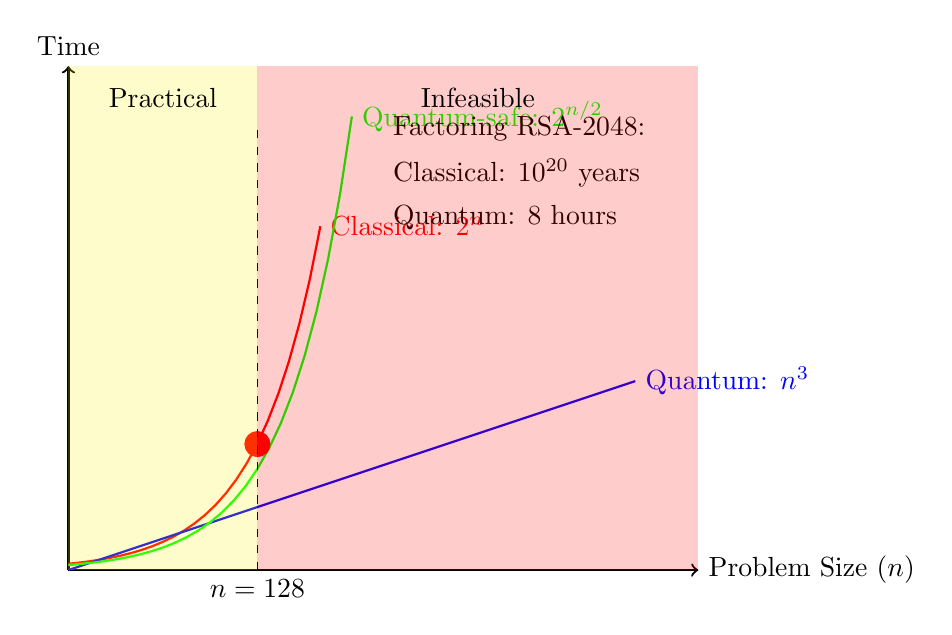
\begin{tikzpicture}[
    scale=0.8,
    axis/.style={->, thick},
    classical/.style={thick, red},
    quantum/.style={thick, blue},
    safe/.style={thick, green}
]
    % Axes
    \draw[axis] (0,0) -- (10,0) node[right] {Problem Size $(n)$};
    \draw[axis] (0,0) -- (0,8) node[above] {Time};
    
    % Classical exponential
    \draw[classical, domain=0:4] plot (\x, {0.1*exp(\x)}) node[right] {Classical: $2^n$};
    
    % Quantum polynomial
    \draw[quantum] (0,0) -- (9,3) node[right] {Quantum: $n^3$};
    
    % Quantum-safe (still exponential)
    \draw[safe, domain=0:4.5] plot (\x, {0.08*exp(\x)}) node[right] {Quantum-safe: $2^{n/2}$};
    
    % Specific points
    \node[circle, fill=red] at (3,2) {};
    \node[below] at (3,0) {$n=128$};
    \draw[dashed] (3,0) -- (3,7);
    
    % Time comparisons
    \node[align=left, anchor=west] at (5,7) {Factoring RSA-2048:};
    \node[align=left, anchor=west] at (5,6.3) {Classical: $10^{20}$ years};
    \node[align=left, anchor=west] at (5,5.6) {Quantum: 8 hours};
    
    % Regions
    \fill[yellow, opacity=0.2] (0,0) rectangle (3,8);
    \fill[red, opacity=0.2] (3,0) rectangle (10,8);
    \node at (1.5,7.5) {Practical};
    \node at (6.5,7.5) {Infeasible};
\end{tikzpicture}
\caption{The exponential-polynomial divide: Where quantum changes everything}
\end{figure}

\paragraph{The Physics Analogy: Computational Energy Barriers}

For physicists, the best analogy is quantum tunneling through energy barriers:

\begin{definition}[Computational Landscape Analogy]
\begin{itemize}
    \item \textbf{Problem space:} Configuration space of possible solutions
    \item \textbf{Computational cost:} Energy barrier height
    \item \textbf{Classical algorithm:} Thermal activation over barrier
    \item \textbf{Quantum algorithm:} Tunneling through barrier
\end{itemize}
\end{definition}

\begin{figure}[h]
\centering
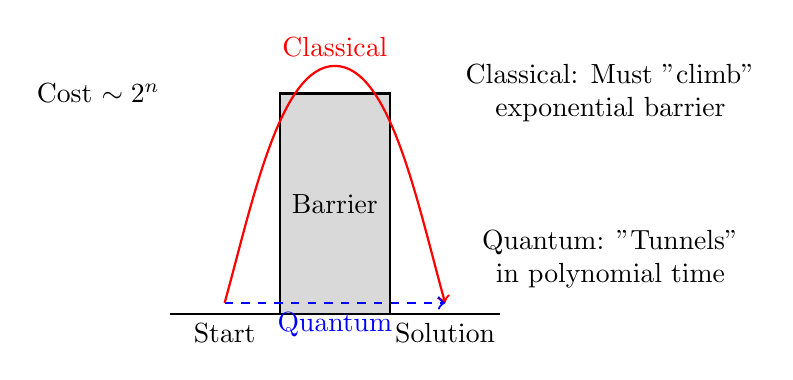
\begin{tikzpicture}[
    scale=0.7,
    barrier/.style={thick},
    classical/.style={->, thick, red},
    quantum/.style={->, thick, blue, dashed}
]
    % Energy barrier
    \draw[barrier] (0,0) -- (2,0) -- (2,4) -- (4,4) -- (4,0) -- (6,0);
    \draw[barrier, fill=gray!30] (2,0) rectangle (4,4);
    
    % Labels
    \node[below] at (1,0) {Start};
    \node[below] at (5,0) {Solution};
    \node at (3,2) {Barrier};
    \node[left] at (0,4) {Cost $\sim 2^n$};
    
    % Classical path
    \draw[classical] (1,0.2) .. controls (1.5,2) and (2,4.5) .. (3,4.5) 
                            .. controls (4,4.5) and (4.5,2) .. (5,0.2);
    \node[above, red] at (3,4.5) {Classical};
    
    % Quantum path
    \draw[quantum] (1,0.2) -- (5,0.2);
    \node[below, blue] at (3,0.2) {Quantum};
    
    % Annotations
    \node[align=center] at (8,4) {Classical: Must "climb"\\exponential barrier};
    \node[align=center] at (8,1) {Quantum: "Tunnels"\\in polynomial time};
\end{tikzpicture}
\caption{Quantum tunneling analogy for algorithmic speedup}
\end{figure}

Just as quantum particles tunnel through classically forbidden regions, quantum algorithms find solutions through classically inaccessible computational paths.

\paragraph{The Hidden Structure: Periodicity}

The quantum advantage isn't universal---it exploits specific mathematical structure:

\begin{theorem}[The Period-Finding Connection]
All three cryptographic problems hide periodic structures:
\begin{enumerate}
    \item \textbf{Factoring:} Find period of $f(x) = a^x \bmod n$
    \item \textbf{Discrete Log:} Find period of $f(j,k) = g^j h^{-k} \bmod p$
    \item \textbf{ECDLP:} Find period in elliptic curve group operations
\end{enumerate}
\end{theorem}

The quantum Fourier transform excels at finding hidden periods:

\begin{algorithm}
\caption{Shor's Algorithm Structure (Simplified)}
\begin{algorithmic}
\State \textbf{Goal:} Factor $n = pq$
\State
\State 1. Choose random $a < n$ with $\gcd(a,n) = 1$
\State 2. Define $f(x) = a^x \bmod n$ (periodic function)
\State 3. \textbf{Quantum step:} Use QFT to find period $r$
\State 4. If $r$ is even and $a^{r/2} \not\equiv -1$:
\State \quad \quad $p = \gcd(a^{r/2} - 1, n)$
\State \quad \quad $q = \gcd(a^{r/2} + 1, n)$
\end{algorithmic}
\end{algorithm}

\paragraph{Why Period Finding is Quantum-Easy}

The quantum advantage comes from superposition and interference:

\begin{enumerate}
    \item \textbf{Superposition:} Evaluate $f(x)$ on all $x$ simultaneously
    \item \textbf{Entanglement:} Create $\sum_x |x\rangle|f(x)\rangle$
    \item \textbf{Measurement:} Collapse to states with same $f(x)$ value
    \item \textbf{Interference:} QFT extracts period from amplitude pattern
\end{enumerate}

Mathematically:
\begin{align}
|\psi\rangle &= \frac{1}{\sqrt{N}} \sum_{x=0}^{N-1} |x\rangle|f(x)\rangle\\
\text{After measuring } f(x) = y: \quad |\psi'\rangle &= \frac{1}{\sqrt{|S_y|}} \sum_{x \in S_y} |x\rangle\\
\text{Where } S_y &= \{x : f(x) = y\} = \{x_0, x_0+r, x_0+2r, ...\}\\
\text{QFT extracts: } &r \text{ (the period)}
\end{align}

\paragraph{Not All Hard Problems Are Quantum-Vulnerable}

Crucially, quantum computers don't make all hard problems easy:

\begin{table}[h]
\centering
\begin{tabular}{|l|l|l|l|}
\hline
\textbf{Problem} & \textbf{Structure} & \textbf{Classical} & \textbf{Quantum} \\
\hline
Integer Factorization & Hidden period & Exponential & Polynomial \\
Discrete Logarithm & Hidden period & Exponential & Polynomial \\
\hline
Shortest Vector (Lattice) & Geometric & Exponential & Still exponential$^*$ \\
Subset Sum (General) & Combinatorial & Exponential & Square root speedup \\
SAT (Boolean) & Constraint & Exponential & Square root speedup \\
\hline
\end{tabular}
\caption{Not all hard problems have exploitable quantum structure. $^*$Best known}
\end{table}

\paragraph{The Quantum Algorithm Paradigm}

Quantum advantage requires problems with specific properties:

\begin{definition}[Quantum-Exploitable Structure]
A problem admits substantial quantum speedup if it has:
\begin{enumerate}
    \item \textbf{Hidden periodicity:} Shor's algorithm applies
    \item \textbf{Hidden subgroup:} Generalization of periodicity
    \item \textbf{Unstructured search:} Grover gives square root speedup
    \item \textbf{Quantum simulation:} Natural quantum problems
\end{enumerate}
\end{definition}

Problems without these structures remain hard:
\begin{itemize}
    \item \textbf{Random-looking problems:} No pattern to exploit
    \item \textbf{High-dimensional geometry:} Lattice problems
    \item \textbf{Non-linear structures:} Multivariate polynomials
    \item \textbf{Hash functions:} Only Grover speedup (manageable)
\end{itemize}

\paragraph{What Makes a Problem Quantum-Safe?}

Post-quantum cryptography seeks problems that resist quantum attack:

\begin{enumerate}
    \item \textbf{No hidden period:} Defeats Shor-like algorithms
    \item \textbf{No efficient quantum representation:} States grow exponentially
    \item \textbf{Classical-quantum gap minimal:} At most polynomial speedup
    \item \textbf{Grover-resistant parameters:} Account for square root speedup
\end{enumerate}

\begin{example}[Why Lattices Resist Quantum Attack]
Shortest Vector Problem in lattices:
\begin{itemize}
    \item No known periodic structure
    \item Geometric problem in high dimensions
    \item Best quantum algorithm: Minor speedup over classical
    \item Believed quantum-hard for decades
\end{itemize}
\end{example}

\paragraph{The Fundamental Divide}

The classical-quantum divide for our three problems is absolute:

\begin{align}
\text{RSA-2048 factoring:} \quad &\text{Classical: } 10^{20} \text{ years}\\
&\text{Quantum: } 8 \text{ hours}\\
\text{Speedup factor:} \quad &10^{24} \times
\end{align}

This isn't an engineering improvement---it's a paradigm shift. No amount of classical optimization can bridge this gap.

\begin{remark}[A Physicist's Perspective]
Just as quantum mechanics revealed that classical physics fundamentally cannot explain certain phenomena (blackbody radiation, photoelectric effect), quantum computing reveals that classical computation fundamentally cannot efficiently solve certain problems. The periodicity in factoring/discrete log is like a "computational quantum phenomenon"---invisible to classical algorithms but obvious to quantum ones.
\end{remark}

This divide explains why post-quantum cryptography cannot simply use "bigger keys" for RSA or elliptic curves. The exponential-to-polynomial collapse is too severe. We need fundamentally different mathematical foundations---problems that remain exponentially hard even for quantum computers. Next, we'll see why lattice problems provide exactly this quantum resistance.

%==================================================
\section{The Quantum Threat and PQC Landscape}
\label{sec:quantum-threat}

\subsection{Quantum Algorithms Breaking Classical Crypto}
\label{sec:quantum-algorithms}

\subsubsection{Shor's Algorithm: The Cryptographic Killer}

Let me dispel a dangerous misconception immediately: Shor's algorithm does not try all possible factors in parallel. This naive view---that quantum computers are just massively parallel classical computers---fundamentally misunderstands both the algorithm and the quantum threat. Shor's algorithm does something far more subtle and devastating: it transforms the factoring problem into finding hidden periods, then exploits quantum interference to extract these periods efficiently.

\paragraph{The Period-Finding Paradigm}

The genius of Shor's algorithm lies in recognizing that factoring hides a periodic structure that quantum computers can detect through interference---much like how a diffraction grating reveals the wavelength of light.

\begin{definition}[The Period-Finding Problem]
Given a function $f: \mathbb{Z} \to \mathbb{Z}$ with hidden period $r$ (i.e., $f(x) = f(x+r)$ for all $x$), find the smallest positive $r$.
\end{definition}

Classically, finding periods requires evaluating $f$ at many points---essentially $O(\sqrt{r})$ evaluations for a period of size $r$. But quantum mechanically, we can create a superposition over all function values and use interference to extract the period in polynomial time.

\begin{figure}[h]
\centering
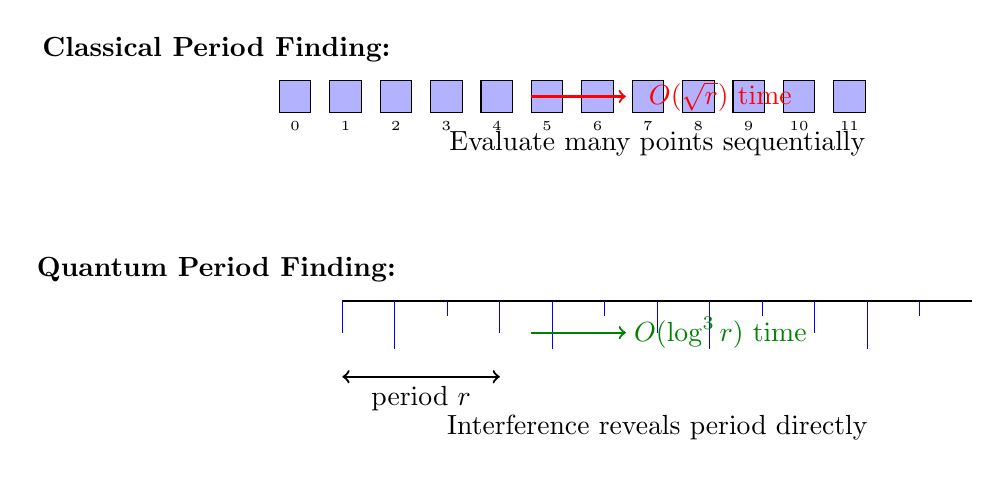
\begin{tikzpicture}[scale=0.8]
    % Classical approach
    \node at (-2, 3) {\textbf{Classical Period Finding:}};
    \foreach \x in {0,1,2,3,4,5,6,7,8,9,10,11} {
        \draw[fill=blue!30] (\x*0.8-1, 2) rectangle (\x*0.8-0.5, 2.5);
        \node[below] at (\x*0.8-0.75, 2) {\tiny \x};
    }
    \node at (5, 1.5) {Evaluate many points sequentially};
    \draw[->, red, thick] (3, 2.25) -- (4.5, 2.25);
    \node[red] at (6, 2.25) {$O(\sqrt{r})$ time};
    
    % Quantum approach
    \node at (-2, -0.5) {\textbf{Quantum Period Finding:}};
    \draw[thick] (0, -1) -- (10, -1);
\foreach \x in {0,1,2,3,4,5,6,7,8,9,10,11} {
    \draw[blue] (\x*0.833, -1) -- (\x*0.833, {-1.5-0.3*sin(\x*120)});
}
    \draw[<->, thick] (0, -2.2) -- (2.5, -2.2);
    \node[below] at (1.25, -2.2) {period $r$};
    \node at (5, -3) {Interference reveals period directly};
    \draw[->, green!50!black, thick] (3, -1.5) -- (4.5, -1.5);
    \node[green!50!black] at (6, -1.5) {$O(\log^3 r)$ time};
\end{tikzpicture}
\caption{Classical sampling vs. quantum interference for period finding}
\end{figure}

The physics analogy is precise: just as optical interference patterns reveal spatial periodicity, quantum interference reveals computational periodicity. The Quantum Fourier Transform (QFT) acts like a computational diffraction grating.

\paragraph{From Factoring to Period Finding}

Here's the critical insight that makes factoring quantum-easy:

\begin{theorem}[Factoring Reduces to Period Finding]
To factor $n = pq$:
\begin{enumerate}
    \item Choose random $a$ with $\gcd(a,n) = 1$
    \item Find the period $r$ of $f(x) = a^x \bmod n$
    \item If $r$ is even and $a^{r/2} \not\equiv -1 \pmod{n}$:
    \begin{itemize}
        \item $\gcd(a^{r/2} - 1, n)$ gives a nontrivial factor
        \item Success probability $\geq 1/2$ for random $a$
    \end{itemize}
\end{enumerate}
\end{theorem}

\begin{proof}[Proof Sketch]
Since $a^r \equiv 1 \pmod{n}$, we have $(a^{r/2})^2 \equiv 1 \pmod{n}$, so:
\begin{align}
(a^{r/2} - 1)(a^{r/2} + 1) &\equiv 0 \pmod{n}
\end{align}
If $a^{r/2} \not\equiv \pm 1 \pmod{n}$, then $a^{r/2} - 1$ shares a nontrivial factor with $n$.
\end{proof}

\begin{algorithm}
\caption{Shor's Algorithm for Integer Factorization}
\label{alg:shor}
\begin{algorithmic}[1]
\Require $n = pq$ (semiprime to factor)
\Ensure Factors $p, q$
\State Choose random $a \in \{2, ..., n-1\}$
\State Compute $g = \gcd(a, n)$ classically
\If{$g > 1$}
    \State \Return $g$ and $n/g$ \Comment{Lucky! Found factor classically}
\EndIf
\State \textbf{Quantum Period Finding:}
\State \quad Initialize quantum registers: $|0\rangle^{\otimes m}|0\rangle^{\otimes n}$
\State \quad Create superposition: $\frac{1}{\sqrt{2^m}} \sum_{x=0}^{2^m-1} |x\rangle|0\rangle$
\State \quad Compute $f(x) = a^x \bmod n$ in second register
\State \quad Measure second register (collapses to periodic subset)
\State \quad Apply QFT to first register
\State \quad Measure first register → get value $y$
\State \quad Use continued fractions on $y/2^m$ to find period $r$
\If{$r$ is even and $a^{r/2} \not\equiv -1 \pmod{n}$}
    \State \Return $\gcd(a^{r/2} - 1, n)$ and $\gcd(a^{r/2} + 1, n)$
\Else
    \State Retry with different $a$
\EndIf
\end{algorithmic}
\end{algorithm}

\paragraph{Concrete Example: Factoring 15}

Let's factor $n = 15$ step by step to see the algorithm in action:

\begin{example}[Factoring 15 with Shor's Algorithm]
\textbf{Step 1:} Choose $a = 7$ (random choice with $\gcd(7, 15) = 1$)

\textbf{Step 2:} We need the period of $f(x) = 7^x \bmod 15$:
\begin{align}
7^0 &\equiv 1 \pmod{15}\\
7^1 &\equiv 7 \pmod{15}\\
7^2 &\equiv 49 \equiv 4 \pmod{15}\\
7^3 &\equiv 28 \equiv 13 \pmod{15}\\
7^4 &\equiv 91 \equiv 1 \pmod{15}
\end{align}
Period $r = 4$ (since $7^4 \equiv 7^0 \pmod{15}$)

\textbf{Step 3:} Quantum circuit finds $r = 4$ through interference:
\begin{center}
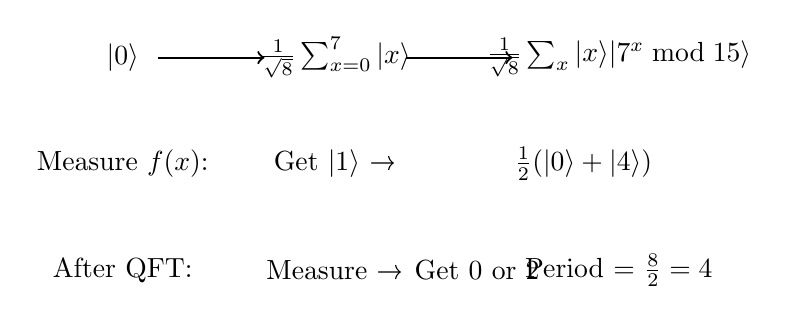
\begin{tikzpicture}[scale=0.9]
    % Quantum state evolution
    \node at (0, 2) {$|0\rangle$};
    \draw[->, thick] (0.5, 2) -- (2, 2);
    \node at (3, 2) {$\frac{1}{\sqrt{8}}\sum_{x=0}^{7}|x\rangle$};
    \draw[->, thick] (4, 2) -- (5.5, 2);
    \node at (7, 2) {$\frac{1}{\sqrt{8}}\sum_{x}|x\rangle|7^x \bmod 15\rangle$};
    
    % After measurement
    \node at (0, 0.5) {Measure $f(x)$:};
    \node at (3, 0.5) {Get $|1\rangle$ →};
    \node at (6.5, 0.5) {$\frac{1}{2}(|0\rangle + |4\rangle)$};
    
    % QFT result
    \node at (0, -1) {After QFT:};
    \node at (3, -1) {Measure →};
    \node at (5, -1) {Get $0$ or $2$};
    \node at (7, -1) {Period = $\frac{8}{2} = 4$};
\end{tikzpicture}
\end{center}

\textbf{Step 4:} Classical post-processing:
\begin{itemize}
    \item $r = 4$ is even \checkmark
    \item $a^{r/2} = 7^2 = 49 \equiv 4 \pmod{15}$
    \item $4 \not\equiv -1 \pmod{15}$ \checkmark
    \item $\gcd(7^2 - 1, 15) = \gcd(48, 15) = 3$
    \item $\gcd(7^2 + 1, 15) = \gcd(50, 15) = 5$
\end{itemize}

\textbf{Result:} $15 = 3 \times 5$ \checkmark
\end{example}

\paragraph{The Quantum Circuit Architecture}

The actual quantum circuit for Shor's algorithm requires precise resource accounting:

\begin{figure}[h]
\centering
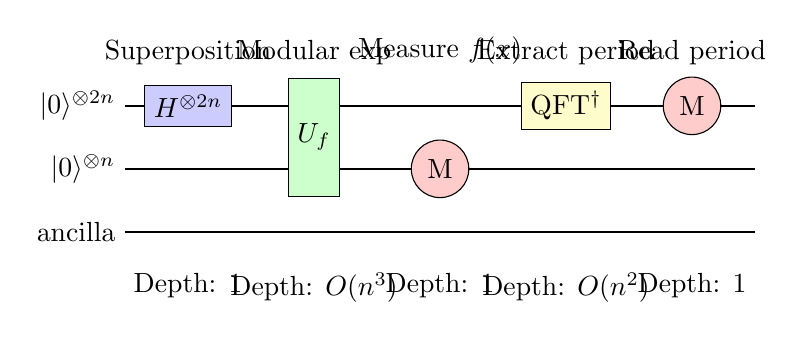
\begin{tikzpicture}[scale=0.8]
    % Registers
    \draw[thick] (0, 2) -- (10, 2);
    \draw[thick] (0, 1) -- (10, 1);
    \draw[thick] (0, 0) -- (10, 0);
    
    \node[left] at (0, 2) {$|0\rangle^{\otimes 2n}$};
    \node[left] at (0, 1) {$|0\rangle^{\otimes n}$};
    \node[left] at (0, 0) {ancilla};
    
    % Gates
    \node[draw, rectangle, fill=blue!20] at (1, 2) {$H^{\otimes 2n}$};
    \node[draw, rectangle, fill=green!20, minimum height=1.5cm] at (3, 1.5) {$U_f$};
    \node[draw, circle, fill=red!20] at (5, 1) {M};
    \node[draw, rectangle, fill=yellow!20] at (7, 2) {QFT$^{\dagger}$};
    \node[draw, circle, fill=red!20] at (9, 2) {M};
    
    % Labels
    \node[above] at (1, 2.5) {Superposition};
    \node[above] at (3, 2.5) {Modular exp};
    \node[above] at (5, 2.5) {Measure $f(x)$};
    \node[above] at (7, 2.5) {Extract period};
    \node[above] at (9, 2.5) {Read period};
    
    % Depth annotations
    \node[below] at (1, -0.5) {Depth: 1};
    \node[below] at (3, -0.5) {Depth: $O(n^3)$};
    \node[below] at (5, -0.5) {Depth: 1};
    \node[below] at (7, -0.5) {Depth: $O(n^2)$};
    \node[below] at (9, -0.5) {Depth: 1};
\end{tikzpicture}
\caption{High-level quantum circuit for Shor's algorithm with depth annotations}
\end{figure}

\begin{remark}[Logical vs Physical Qubits]
Critical distinction for realistic assessment:
\begin{itemize}
    \item \textbf{Logical qubits:} Error-free qubits in the algorithm
    \item \textbf{Physical qubits:} Noisy qubits in actual hardware
    \item \textbf{Error correction overhead:} $\sim$1,000-10,000 physical per logical
    \item \textbf{Current state (2025):} $\sim$1,000 physical qubits, 0 logical qubits
\end{itemize}
\end{remark}

For factoring an $n$-bit number:
\begin{itemize}
    \item \textbf{Logical qubits:} $3n + O(\log n)$
    \item \textbf{Quantum gates:} $O(n^3)$ (dominated by modular exponentiation)
    \item \textbf{Circuit depth:} $O(n^3)$ 
    \item \textbf{Classical runtime:} $O(n^3)$ for polynomial-time quantum circuits
    \item \textbf{Physical qubits (with error correction):}
    \begin{itemize}
        \item Conservative: $\sim$10,000 physical per logical
        \item Optimistic: $\sim$1,000 physical per logical
        \item For RSA-2048: 20-200 million physical qubits
    \end{itemize}
\end{itemize}

\begin{remark}[Breaking RSA-2048: Reality Check]
The "8 hours" claim assumes:
\begin{itemize}
    \item Logical qubits with perfect gates (not physical qubits)
    \item Clock speed of $\sim$1 MHz for quantum operations
    \item No decoherence or error correction overhead
    \item Efficient classical control systems
\end{itemize}
With realistic error correction and current parameters, breaking RSA-2048 would require:
\begin{itemize}
    \item $\sim$4,000 logical qubits
    \item $\sim$20 million physical qubits (conservative)
    \item $\sim$8 hours of coherent quantum computation
    \item Technology gap: 4-5 orders of magnitude from current systems
\end{itemize}
\end{remark}

\paragraph{Impact Analysis: The Dual Catastrophe}

Here's what many miss: Shor's algorithm doesn't just break encryption---it equally devastates digital signatures:

\begin{table}[h]
\centering
\begin{tabular}{|l|c|c|l|}
\hline
\textbf{Algorithm} & \textbf{Purpose} & \textbf{Broken?} & \textbf{Impact} \\
\hline
RSA-2048 & Encryption & \xmark & No confidentiality \\
RSA-2048 & Signatures & \xmark & No authentication \\
ECDH-P256 & Key exchange & \xmark & No secure channels \\
ECDSA-P256 & Signatures & \xmark & No identity verification \\
DSA & Signatures & \xmark & No integrity protection \\
\hline
AES-128 & Encryption & ↓ & Reduced to 64-bit security \\
SHA-256 & Hashing & ↓ & Reduced to 128-bit security \\
\hline
\end{tabular}
\caption{Shor's algorithm breaks all asymmetric cryptography, not just encryption}
\end{table}

\begin{example}[Breaking Digital Signatures with Shor]
Given ECDSA public key $Q = dG$ on curve with order $n$:
\begin{enumerate}
    \item Use Shor to solve discrete log: find $d$ from $Q = dG$
    \item Now you have the private key $d$
    \item Forge any signature: $s = k^{-1}(h + rd) \bmod n$
    \item Result: Perfect impersonation of key owner
\end{enumerate}
Time required: Same as breaking encryption (polynomial in key size)
\end{example}

\paragraph{Timeline and the "Harvest Now, Decrypt Later" Threat}

The timeline creates an unusual situation in cryptography:

\begin{itemize}
    \item \textbf{Today (2025):} No quantum computer can run Shor's algorithm at scale
    \item \textbf{2033:} IBM roadmap targets 100,000 physical qubits
    \item \textbf{2035-2040:} Possible threshold for logical qubits via error correction
    \item \textbf{Critical insight:} Data encrypted today can be stored and decrypted later
\end{itemize}

\begin{remark}[The Retrospective Threat]
If your encrypted data has value for 10+ years, it's already at risk:
\begin{itemize}
    \item Government secrets (25-50 year classification)
    \item Medical records (lifetime + 10 years)
    \item Financial records (7-10 years regulatory)
    \item Industrial IP (20+ year patents)
    \item Personal communications (lifetime privacy)
\end{itemize}
Adversaries are likely harvesting encrypted data now for future decryption. This isn't paranoia---it's documented in national security assessments.
\end{remark}

\begin{figure}[h]
\centering
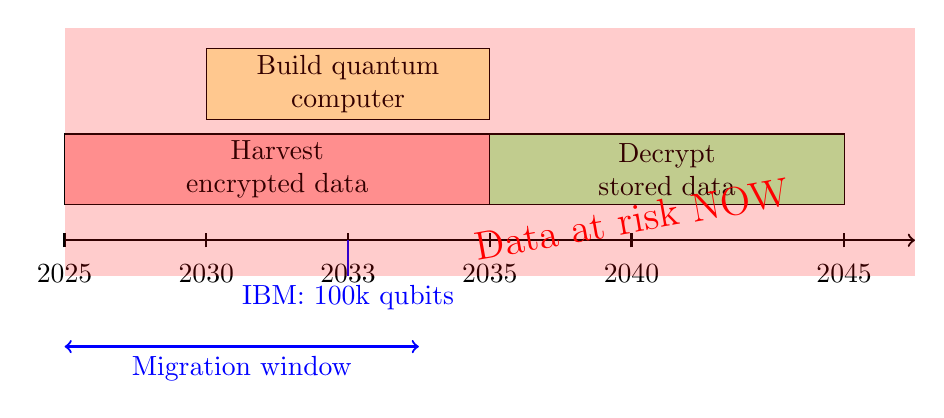
\begin{tikzpicture}[scale=0.9]
    % Timeline
    \draw[thick, ->] (0, 0) -- (12, 0);
    \foreach \x/\year in {0/2025, 2/2030, 4/2033, 6/2035, 8/2040, 11/2045} {
        \draw[thick] (\x, -0.1) -- (\x, 0.1);
        \node[below] at (\x, -0.2) {\year};
    }
    
    % Events
    \draw[fill=red!30] (0, 0.5) rectangle (6, 1.5);
    \node[align=center] at (3, 1) {Harvest\\encrypted data};
    
    \draw[fill=yellow!30] (2, 1.7) rectangle (6, 2.7);
    \node[align=center] at (4, 2.2) {Build quantum\\computer};
    
    \draw[fill=green!30] (6, 0.5) rectangle (11, 1.5);
    \node[align=center] at (8.5, 1) {Decrypt\\stored data};
    
    % IBM milestone
    \draw[thick, blue] (4, -0.5) -- (4, 0);
    \node[below, blue] at (4, -0.5) {IBM: 100k qubits};
    
    % Migration window
    \draw[<->, thick, blue] (0, -1.5) -- (5, -1.5);
    \node[below, blue] at (2.5, -1.5) {Migration window};
    
    % Risk zone
    \fill[red, opacity=0.2] (0, -0.5) rectangle (12, 3);
    \node[red, rotate=10] at (8, 0.3) {\Large Data at risk NOW};
\end{tikzpicture}
\caption{The harvest now, decrypt later timeline aligned with quantum roadmaps}
\end{figure}

\paragraph{Why No Classical Algorithm Can Compete}

The quantum advantage for factoring is absolute, not incremental:

\begin{align}
\text{Best classical (GNFS):} \quad &L_n[1/3, (64/9)^{1/3}] \approx \exp(1.9 \cdot n^{1/3} \cdot (\log n)^{2/3})\\
\text{Shor's algorithm (quantum):} \quad &O(n^3) \text{ quantum operations}\\
\text{For RSA-2048:} \quad &\text{Classical: } 10^{20} \text{ years vs. Quantum: } 8 \text{ hours}^*
\end{align}
*With perfect logical qubits; see reality check above for physical requirements.

This is not a speedup that Moore's Law can address. If classical computers became $10^{10}$ times faster, factoring RSA-2048 would still take a billion years. The quantum computer doesn't work harder---it works differently.

\begin{remark}[A Physicist's Perspective]
Think of it this way: classical algorithms must explore an exponentially large solution space, like a particle diffusing through a vast energy landscape. Quantum algorithms use interference to "tunnel" directly to the solution, bypassing the exponential search entirely. It's not about speed---it's about taking a fundamentally different path through the computation.
\end{remark}

The implications are stark: every RSA key, every ECDSA signature, every Diffie-Hellman exchange will become breakable. Not weakened---completely broken. This isn't a distant theoretical threat; it's an engineering challenge that billions of dollars are actively solving. The only question is when, not if.

With this existential threat to asymmetric cryptography established, we now turn to the more subtle challenge that quantum computers pose to symmetric systems.

\subsubsection{Grover's Algorithm: The Symmetric Threat}

While Shor's algorithm gets the headlines---"Quantum computers will break all encryption!"---Grover's algorithm poses a more subtle threat. It doesn't obliterate symmetric cryptography the way Shor destroys RSA, but it does weaken it significantly. The good news: this weakening is predictable, bounded, and manageable. The bad news: many people either ignore it entirely or wildly overestimate what it can do.

\paragraph{The Unstructured Search Problem}

Grover's algorithm solves a deceptively simple problem:

\begin{definition}[Unstructured Search]
Given a function $f: \{0,1\}^n \to \{0,1\}$ (a "black box" oracle) where exactly one input $x^*$ satisfies $f(x^*) = 1$, find $x^*$.
\end{definition}

Classically, this is the ultimate needle-in-a-haystack problem. With no structure to exploit, you must check inputs one by one:

\begin{itemize}
    \item \textbf{Classical:} Expected $2^{n-1}$ evaluations (half the search space)
    \item \textbf{Quantum:} Only $\frac{\pi}{4}\sqrt{2^n} \approx 0.785 \cdot 2^{n/2}$ evaluations
    \item \textbf{Speedup:} Quadratic (square root)
\end{itemize}

\begin{example}[Concrete Impact on Search]
Breaking a 128-bit key:
\begin{itemize}
    \item Classical: $2^{127} \approx 10^{38}$ operations (impossible)
    \item Quantum: $2^{64} \approx 10^{19}$ operations (difficult but feasible)
    \item Mitigation: Use 256-bit key → $2^{128}$ quantum operations (safe again)
\end{itemize}
\end{example}

\begin{remark}[Why Grover Doesn't Threaten Asymmetric Crypto]
Students often ask: "Can't Grover search for RSA private keys?" Let's address this immediately:
\begin{itemize}
    \item RSA-2048 private key space: $\sim 2^{2048}$
    \item Grover speedup: $2^{1024}$ quantum operations
    \item Universe lifetime: $\sim 2^{60}$ nanoseconds
    \item Still need $2^{964}$ universe lifetimes!
\end{itemize}
Grover provides only quadratic speedup---insufficient to overcome exponential key spaces in asymmetric cryptography. This is why we focus on Shor for asymmetric and Grover for symmetric systems.
\end{remark}

\paragraph{How Grover's Algorithm Works}

Here's the critical insight: Grover's algorithm does NOT check all possibilities in parallel. This misconception leads to confusion about its capabilities and limitations.

\begin{figure}[h]
\centering
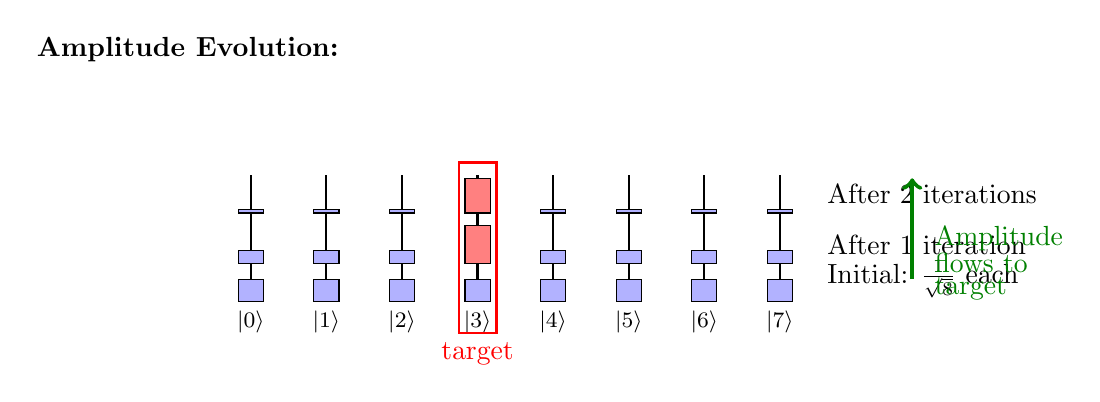
\begin{tikzpicture}[scale=0.8]
    % Initial state
    \node at (-1, 4) {\textbf{Amplitude Evolution:}};
    
    % States
    \foreach \i in {0,1,2,3,4,5,6,7} {
        \draw[thick] (\i*1.2, 0) -- (\i*1.2, 2);
        \node[below] at (\i*1.2, 0) {\footnotesize $|\i\rangle$};
    }
    
    % Initial amplitude
    \foreach \i in {0,1,2,3,4,5,6,7} {
        \draw[fill=blue!30] (\i*1.2-0.2, 0) rectangle (\i*1.2+0.2, 0.35);
    }
    \node[right] at (9, 0.35) {Initial: $\frac{1}{\sqrt{8}}$ each};
    
    % After 1 iteration
    \foreach \i in {0,1,2,4,5,6,7} {
        \draw[fill=blue!30] (\i*1.2-0.2, 0.6) rectangle (\i*1.2+0.2, 0.8);
    }
    \draw[fill=red!50] (3*1.2-0.2, 0.6) rectangle (3*1.2+0.2, 1.2);
    \node[right] at (9, 0.9) {After 1 iteration};
    
    % After 2 iterations
    \foreach \i in {0,1,2,4,5,6,7} {
        \draw[fill=blue!30] (\i*1.2-0.2, 1.4) rectangle (\i*1.2+0.2, 1.45);
    }
    \draw[fill=red!50] (3*1.2-0.2, 1.4) rectangle (3*1.2+0.2, 1.95);
    \node[right] at (9, 1.7) {After 2 iterations};
    
    % Target state marked
    \draw[thick, red] (3*1.2-0.3, -0.5) rectangle (3*1.2+0.3, 2.2);
    \node[below, red] at (3*1.2, -0.5) {target};
    
    % Arrow showing evolution
    \draw[->, ultra thick, green!50!black] (10.5, 0.35) -- (10.5, 1.95);
    \node[right, green!50!black] at (10.7, 1) {Amplitude};
    \node[right, green!50!black] at (10.7, 0.6) {flows to};
    \node[right, green!50!black] at (10.7, 0.2) {target};
\end{tikzpicture}
\caption{Grover's algorithm amplifies the target state's amplitude through interference}
\end{figure}

Instead of parallel search, Grover uses \textbf{amplitude amplification}:

\begin{enumerate}
    \item Start with equal superposition: $|\psi\rangle = \frac{1}{\sqrt{N}} \sum_{x=0}^{N-1} |x\rangle$
    \item Mark the target state by flipping its phase: $|x^*\rangle \to -|x^*\rangle$
    \item Perform "inversion about average" operation
    \item Repeat $\approx \frac{\pi}{4}\sqrt{N}$ times
    \item Measure to get $x^*$ with high probability
\end{enumerate}

The physics analogy: think of a resonant cavity where constructive interference gradually builds up amplitude at the target frequency while destructive interference suppresses others.

\paragraph{The Algorithm in Detail}

\begin{algorithm}
\caption{Grover's Algorithm}
\label{alg:grover}
\begin{algorithmic}[1]
\Require Oracle $O_f$ where $O_f|x\rangle = (-1)^{f(x)}|x\rangle$
\Require Number of items $N = 2^n$
\Ensure Solution $x^*$ where $f(x^*) = 1$
\State Initialize: $|\psi\rangle = H^{\otimes n}|0\rangle^{\otimes n} = \frac{1}{\sqrt{N}} \sum_{x=0}^{N-1} |x\rangle$
\State Set iterations: $k = \lfloor \frac{\pi}{4}\sqrt{N} \rfloor$
\For{$i = 1$ to $k$}
    \State Apply oracle: $|\psi\rangle \gets O_f|\psi\rangle$ \Comment{Flip phase of target}
    \State Apply diffusion: $|\psi\rangle \gets D|\psi\rangle$ \Comment{Inversion about average}
    \State \quad where $D = 2|s\rangle\langle s| - I$ and $|s\rangle = \frac{1}{\sqrt{N}}\sum_x|x\rangle$
\EndFor
\State Measure $|\psi\rangle$ to get $x$
\State Verify: if $f(x) = 1$ return $x$, else repeat
\end{algorithmic}
\end{algorithm}

The Grover operator $G = D \cdot O_f$ has elegant geometric interpretation:

\begin{itemize}
    \item $O_f$: Reflection through hyperplane orthogonal to target
    \item $D$: Reflection through average state
    \item $G$: Rotation in 2D subspace spanned by target and non-target states
    \item Angle of rotation: $\theta = 2\arcsin(1/\sqrt{N})$
\end{itemize}

After $k$ iterations, the amplitude of the target state is:
\begin{equation}
\alpha_k = \sin\left((2k+1)\arcsin(1/\sqrt{N})\right)
\end{equation}

Optimal number of iterations: $k_{\text{opt}} = \lfloor \frac{\pi}{4}\sqrt{N} - \frac{1}{2} \rfloor$

\paragraph{Impact on Symmetric Cryptography}

Let's quantify the concrete impact on real cryptographic primitives:

\begin{table}[h]
\centering
\begin{tabular}{|l|c|c|c|c|}
\hline
\textbf{Algorithm} & \textbf{Classical} & \textbf{Quantum} & \textbf{Effective} & \textbf{Safe?} \\
& \textbf{Security} & \textbf{Attack} & \textbf{Security} & \\
\hline
AES-128 & $2^{128}$ & $2^{64}$ & 64 bits & No \\
AES-192 & $2^{192}$ & $2^{96}$ & 96 bits & Marginal \\
AES-256 & $2^{256}$ & $2^{128}$ & 128 bits & Yes \\
\hline
SHA-256 (collision) & $2^{128}$ & $2^{85.3}$ & 85 bits & No \\
SHA-384 (collision) & $2^{192}$ & $2^{128}$ & 128 bits & Yes \\
SHA-512 (collision) & $2^{256}$ & $2^{170.7}$ & 171 bits & Yes \\
\hline
SHA-256 (preimage) & $2^{256}$ & $2^{128}$ & 128 bits & Yes \\
SHA-512 (preimage) & $2^{512}$ & $2^{256}$ & 256 bits & Yes \\
\hline
\end{tabular}
\caption{Grover's impact on symmetric primitives (Note: collision finding gets $2^{n/3}$ due to BHT algorithm)}
\end{table}

\begin{example}[Breaking AES-128 with Grover]
Given ciphertext $C = \text{AES}_{k}(P)$ where $P$ is known:
\begin{itemize}
    \item Define oracle: $f(k') = \begin{cases} 1 & \text{if } \text{AES}_{k'}(P) = C \\ 0 & \text{otherwise} \end{cases}$
    \item Search space: $2^{128}$ possible keys
    \item Grover iterations needed: $\frac{\pi}{4} \cdot 2^{64} \approx 1.25 \times 10^{19}$
    \item Each iteration: 1 AES encryption + quantum gates
    \item Total time: $\sim 2^{64}$ AES operations
\end{itemize}
This is feasible with a large quantum computer, unlike the classical $2^{128}$.
\end{example}

\paragraph{Why This is Manageable}

Unlike Shor's algorithm, Grover's threat has a simple solution:

\begin{theorem}[Grover's Bounded Impact]
For any function with $n$-bit security against classical attack:
\begin{itemize}
    \item Quantum security: $n/2$ bits
    \item Mitigation: Use $2n$-bit keys
    \item Cost: Linear increase in key size
\end{itemize}
\end{theorem}

Compare the mitigation strategies:

\begin{itemize}
    \item \textbf{Shor's algorithm on RSA:}
    \begin{itemize}
        \item Going from 2048 to 4096 bits: Still broken instantly
        \item Going to 1 million bits: Still polynomial time for quantum
        \item Only solution: Abandon RSA entirely
    \end{itemize}
    \item \textbf{Grover's algorithm on AES:}
    \begin{itemize}
        \item Going from 128 to 256 bits: Full security restored
        \item Cost: 2× key storage, identical performance
        \item Implementation: Change one parameter
    \end{itemize}
\end{itemize}

\paragraph{Practical Implications and Recommendations}

Current guidance for quantum-resistant symmetric cryptography:

\begin{enumerate}
    \item \textbf{Use AES-256} for long-term security
    \begin{itemize}
        \item Already standard in many applications
        \item No performance penalty on modern hardware (AES-NI)
        \item Provides 128-bit post-quantum security
    \end{itemize}
    
    \item \textbf{Use SHA-384 or SHA-512} for hashing
    \begin{itemize}
        \item SHA-256 remains safe for preimage resistance
        \item But use larger variants for collision resistance
        \item SHA-3 family also quantum-resistant with appropriate sizes
    \end{itemize}
    
    \item \textbf{Double MAC key sizes} where feasible
    \begin{itemize}
        \item HMAC-SHA256 with 256-bit keys
        \item Poly1305 remains secure (not searchable)
    \end{itemize}
\end{enumerate}

\begin{table}[h]
\centering
\begin{tabular}{|l|l|l|}
\hline
\textbf{Current Practice} & \textbf{Quantum-Safe} & \textbf{Migration Effort} \\
\hline
AES-128 & AES-256 & Change parameter \\
3DES & AES-256 & Algorithm replacement \\
SHA-1 (broken anyway) & SHA-384 & Algorithm replacement \\
SHA-256 & SHA-256 (preimage) & None needed \\
& SHA-384 (collision) & Change parameter \\
HMAC-SHA256 & HMAC-SHA256 & None (key size ok) \\
ChaCha20 & ChaCha20 & Double key size \\
\hline
\end{tabular}
\caption{Symmetric crypto migration is straightforward}
\end{table}

\paragraph{The Bottom Line on Grover}

Grover's algorithm is the "good news" story of quantum cryptanalysis:

\begin{itemize}
    \item \textbf{Predictable impact:} Exactly square root speedup
    \item \textbf{Simple mitigation:} Double key sizes
    \item \textbf{Already implemented:} AES-256 is standard
    \item \textbf{No algorithm changes:} Same AES, just bigger keys
    \item \textbf{Performance neutral:} Hardware acceleration handles it
    \item \textbf{Future-proof:} No known quantum algorithm beats Grover for unstructured search
\end{itemize}

\begin{example}[Cost of Quantum-Proofing Symmetric Crypto]
Large cloud provider migrating to quantum-safe symmetric crypto:
\begin{itemize}
    \item Current: 10 million AES-128 keys in HSMs
    \item Migration: Update to AES-256
    \item Storage cost: 128 bits × 10M = 160 MB additional
    \item Performance impact: 0\% (AES-NI handles both identically)
    \item Development effort: Update configuration files
    \item Timeline: Can be done incrementally
\end{itemize}
Compare to RSA → PQC migration: New algorithms, protocols, libraries, testing...
\end{example}

\begin{remark}[A Reassuring Perspective]
If Grover's algorithm were the only quantum threat to cryptography, the transition would be trivial. Update some configuration files, double some parameters, and we're done. The real challenge isn't symmetric crypto---it's the complete algorithmic replacement required for public key systems. Grover is quantum computing's warning shot, not its killing blow.
\end{remark}

This manageable threat stands in stark contrast to the existential crisis Shor's algorithm poses for public key cryptography. While we must completely rebuild our asymmetric cryptographic infrastructure, symmetric cryptography needs only minor adjustments. This is why post-quantum cryptography focuses almost exclusively on replacing RSA, Diffie-Hellman, and elliptic curves---the symmetric primitives will survive with minimal changes.

Having examined how quantum algorithms threaten current cryptography, we now turn to the broader landscape of quantum-safe solutions and the crucial differences between physical and mathematical approaches to security.

\subsection{PQC vs QKD: Complementary Not Competing}
\label{sec:pqc-vs-qkd}

\subsubsection{Fundamental Differences}

A dangerous misconception pervades discussions of quantum-safe security: that we must choose between Quantum Key Distribution (QKD) and Post-Quantum Cryptography (PQC). This false dichotomy misunderstands both technologies. QKD and PQC solve different problems, operate on different principles, and have different failure modes. Most critically, QKD \textbf{cannot} provide digital signatures---meaning PQC is mandatory regardless of QKD deployment. Understanding these fundamental differences is crucial for any serious quantum security strategy.

\paragraph{Security Paradigms: Unconditional vs Computational}

The core distinction lies in what provides the security guarantee:

\begin{definition}[Information-Theoretic Security (QKD)]
Security guaranteed by the laws of physics, independent of computational power:
\begin{itemize}
    \item Based on: Quantum mechanics (no-cloning theorem, measurement disturbance)
    \item Broken by: Violating physics or compromising the physical channel
    \item Computational power: Irrelevant---infinite computation doesn't help
\end{itemize}
\end{definition}

\begin{definition}[Computational Security (PQC)]
Security guaranteed by computational hardness, assuming bounded resources:
\begin{itemize}
    \item Based on: Mathematical problems believed hard for quantum computers
    \item Broken by: New algorithms or sufficient computational power
    \item Computational power: Central---more computation weakens security
\end{itemize}
\end{definition}

\begin{figure}[h]
\centering
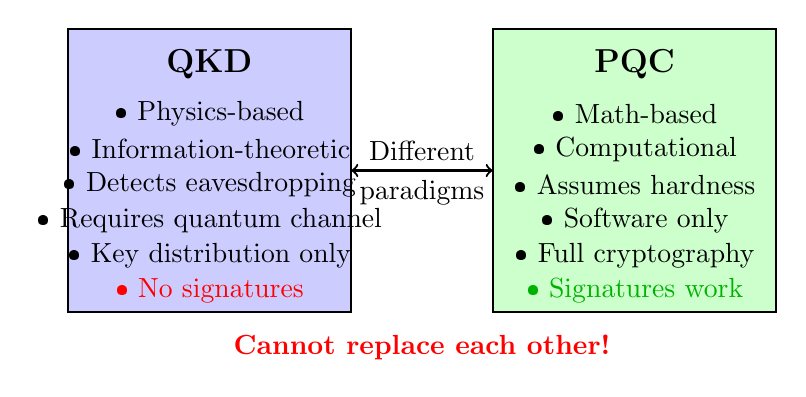
\begin{tikzpicture}[scale=0.9]
    % QKD side
    \draw[thick, fill=blue!20] (-5, 0) rectangle (-1, 4);
    \node[align=center, font=\large\bfseries] at (-3, 3.5) {QKD};
    \node[align=left] at (-3, 2.8) {• Physics-based};
    \node[align=left] at (-3, 2.3) {• Information-theoretic};
    \node[align=left] at (-3, 1.8) {• Detects eavesdropping};
    \node[align=left] at (-3, 1.3) {• Requires quantum channel};
    \node[align=left] at (-3, 0.8) {• Key distribution only};
    \node[align=left, red] at (-3, 0.3) {• No signatures};
    
    % PQC side
    \draw[thick, fill=green!20] (1, 0) rectangle (5, 4);
    \node[align=center, font=\large\bfseries] at (3, 3.5) {PQC};
    \node[align=left] at (3, 2.8) {• Math-based};
    \node[align=left] at (3, 2.3) {• Computational};
    \node[align=left] at (3, 1.8) {• Assumes hardness};
    \node[align=left] at (3, 1.3) {• Software only};
    \node[align=left] at (3, 0.8) {• Full cryptography};
    \node[align=left, green!70!black] at (3, 0.3) {• Signatures work};
    
    % Comparison arrows
    \draw[<->, thick] (-1, 2) -- (1, 2);
    \node[above] at (0, 2) {Different};
    \node[below] at (0, 2) {paradigms};
    
    % Bottom emphasis
    \node[align=center, font=\bfseries, red] at (0, -0.5) {Cannot replace each other!};
\end{tikzpicture}
\caption{QKD and PQC: Fundamentally different approaches to quantum-safe security}
\end{figure}

Neither paradigm is inherently superior---they protect against different threat models:

\begin{itemize}
    \item \textbf{QKD wins when:} Adversary has unlimited computation but must obey physics
    \item \textbf{PQC wins when:} You need signatures, internet-scale deployment, or software-only solutions
    \item \textbf{Both needed when:} Protecting ultra-high-value secrets for decades
\end{itemize}

\paragraph{Physical vs Mathematical Protection}

The infrastructure requirements create a stark divide:

\begin{table}[h]
\centering
\begin{tabular}{|l|l|l|}
\hline
\textbf{Requirement} & \textbf{QKD} & \textbf{PQC} \\
\hline
Physical channel & Dedicated fiber/free-space & Any channel \\
Distance limit & $\sim$100-200 km (fiber) & Unlimited \\
Trusted repeaters & Required for long distance & Not needed \\
Quantum hardware & Single-photon sources/detectors & None \\
Classical hardware & Control electronics & Standard CPU \\
Cost per link & \$100,000+ & \$0 (software) \\
Deployment time & Months (fiber installation) & Minutes (software update) \\
Maintenance & Specialized technicians & Standard IT \\
\hline
\end{tabular}
\caption{Infrastructure requirements: QKD needs physics, PQC needs mathematics}
\end{table}

\begin{example}[Real QKD Deployment]
Swiss government QKD network protecting Geneva elections:
\begin{itemize}
    \item Distance: 29 km dedicated fiber
    \item Cost: \$10 million+ 
    \item Speed: 1.4 Mbps key generation
    \item Availability: 99.9\% (weather affects free-space backup)
    \item Limitation: Only connects specific government buildings
    \item Still needs: Classical crypto for authentication and signatures!
\end{itemize}
\end{example}

\paragraph{The Scalability Divide}

The physical nature of QKD creates fundamental scalability limits:

\begin{figure}[h]
\centering
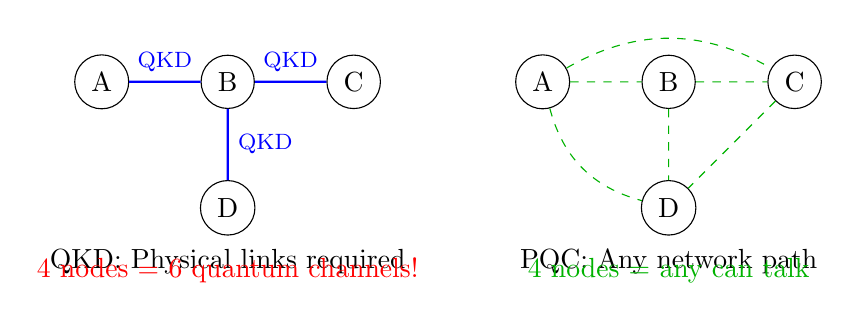
\begin{tikzpicture}[scale=0.8]
    % QKD network
    \node[draw, circle] (a1) at (0, 2) {A};
    \node[draw, circle] (b1) at (2, 2) {B};
    \node[draw, circle] (c1) at (4, 2) {C};
    \node[draw, circle] (d1) at (2, 0) {D};
    
    \draw[thick, blue] (a1) -- node[above, font=\footnotesize] {QKD} (b1);
    \draw[thick, blue] (b1) -- node[above, font=\footnotesize] {QKD} (c1);
    \draw[thick, blue] (b1) -- node[right, font=\footnotesize] {QKD} (d1);
    
    \node[below] at (2, -0.5) {QKD: Physical links required};
    \node[red] at (2, -1) {4 nodes = 6 quantum channels!};
    
    % PQC network
    \node[draw, circle] (a2) at (7, 2) {A};
    \node[draw, circle] (b2) at (9, 2) {B};
    \node[draw, circle] (c2) at (11, 2) {C};
    \node[draw, circle] (d2) at (9, 0) {D};
    
    \draw[dashed, green!70!black] (a2) -- (b2);
    \draw[dashed, green!70!black] (b2) -- (c2);
    \draw[dashed, green!70!black] (b2) -- (d2);
    \draw[dashed, green!70!black] (a2) to[bend left] (c2);
    \draw[dashed, green!70!black] (a2) to[bend right] (d2);
    \draw[dashed, green!70!black] (c2) -- (d2);
    
    \node[below] at (9, -0.5) {PQC: Any network path};
    \node[green!70!black] at (9, -1) {4 nodes = any can talk};
\end{tikzpicture}
\caption{QKD requires dedicated point-to-point links; PQC works over any network}
\end{figure}

For $n$ parties to communicate with QKD:
\begin{itemize}
    \item Required quantum channels: $\binom{n}{2} = \frac{n(n-1)}{2}$
    \item For 1,000 users: 499,500 quantum channels needed!
    \item Alternative: Trusted relay nodes (but this weakens security model)
    \item Reality: QKD works for specific high-value point-to-point links
\end{itemize}

\paragraph{The Authentication Paradox}

Here's the dirty secret of QKD that vendors don't emphasize:

\begin{theorem}[QKD Authentication Requirement]
QKD is \textbf{unconditionally secure} against eavesdropping but \textbf{completely insecure} against man-in-the-middle attacks without pre-existing authentication.
\end{theorem}

\begin{figure}[h]
\centering
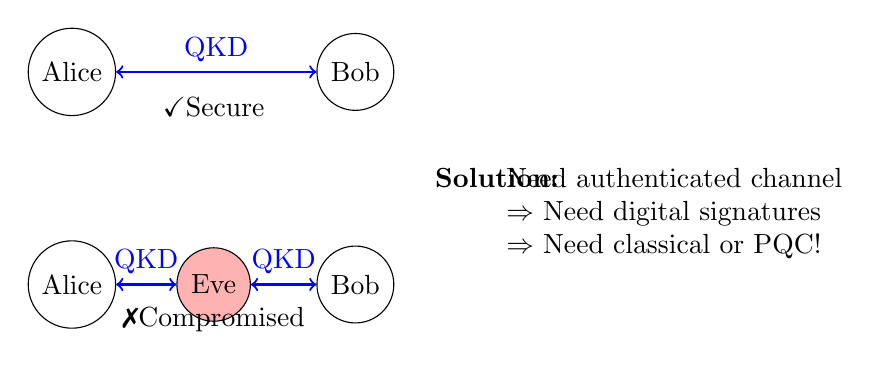
\begin{tikzpicture}[scale=0.9]
    % Legitimate QKD
    \node[draw, circle] (alice1) at (0, 2) {Alice};
    \node[draw, circle] (bob1) at (4, 2) {Bob};
    \draw[thick, blue, <->] (alice1) -- node[above] {QKD} (bob1);
    \node at (2, 1.5) {\checkmark Secure};
    
    % MITM attack
    \node[draw, circle] (alice2) at (0, -1) {Alice};
    \node[draw, circle, fill=red!30] (eve) at (2, -1) {Eve};
    \node[draw, circle] (bob2) at (4, -1) {Bob};
    \draw[thick, blue, <->] (alice2) -- node[above] {QKD} (eve);
    \draw[thick, blue, <->] (eve) -- node[above] {QKD} (bob2);
    \node at (2, -1.5) {\xmark Compromised};
    
    % Solution
    \node at (6, 0.5) {\textbf{Solution:}};
    \node[align=left] at (8.5, 0) {Need authenticated channel\\
    $\Rightarrow$ Need digital signatures\\
    $\Rightarrow$ Need classical or PQC!};
\end{tikzpicture}
\caption{QKD's bootstrapping problem: Secure key exchange requires prior authentication}
\end{figure}

The authentication options:
\begin{enumerate}
    \item \textbf{Pre-shared keys:} Defeats the purpose (if you can share keys, why QKD?)
    \item \textbf{Classical signatures:} Vulnerable to quantum computers
    \item \textbf{PQC signatures:} Quantum-safe but admits QKD isn't sufficient alone
\end{enumerate}

\paragraph{The Missing Piece: Digital Signatures}

This is the killer limitation that many overlook:

\begin{remark}[Critical Limitation]
\textbf{QKD cannot, even in principle, provide digital signatures.} Signatures require:
\begin{itemize}
    \item Public verifiability (anyone can verify)
    \item Non-repudiation (signer cannot deny)
    \item Transferability (signature remains valid when forwarded)
\end{itemize}
QKD provides none of these. It only distributes secret keys between two parties.
\end{remark}

Consider what needs signatures in practice:
\begin{itemize}
    \item \textbf{Software updates:} How do you verify legitimate code?
    \item \textbf{Certificates:} How do you authenticate websites?
    \item \textbf{Financial transactions:} How do you prove authorization?
    \item \textbf{Legal documents:} How do you create binding agreements?
    \item \textbf{Email:} How do you verify sender identity?
\end{itemize}

\begin{example}[The Signature Gap]
Scenario: Bank wants quantum-safe communication with customers
\begin{itemize}
    \item QKD can: Distribute keys to encrypt account data
    \item QKD cannot: Sign transaction authorizations
    \item QKD cannot: Authenticate the bank's website
    \item QKD cannot: Verify customer's identity
    \item Result: Must use PQC for signatures regardless
\end{itemize}
\end{example}

\paragraph{Practical Deployment Reality}

Let's be brutally honest about deployment challenges:

\begin{table}[h]
\centering
\begin{tabular}{|l|p{5cm}|p{5cm}|}
\hline
\textbf{Factor} & \textbf{QKD Reality} & \textbf{PQC Reality} \\
\hline
\textbf{Cost} & \$50k-500k per link & Free (software update) \\
\textbf{Distance} & 100km without repeaters & Global (Internet) \\
\textbf{Speed} & kbps to Mbps key rate & Gbps data rate \\
\textbf{Integration} & Requires new infrastructure & Uses existing networks \\
\textbf{Maintenance} & Quantum physicists on call & Standard IT staff \\
\textbf{Reliability} & 99-99.9\% (environmental) & 99.999\%+ (software) \\
\textbf{Scalability} & Point-to-point only & Billions of endpoints \\
\hline
\end{tabular}
\caption{Deployment reality: QKD for specific links, PQC for everything}
\end{table}

\begin{example}[Cost Analysis: Securing a Corporate Network]
Medium enterprise with 10 offices wanting quantum-safe security:

\textbf{QKD Approach:}
\begin{itemize}
    \item 45 quantum channels needed (full mesh)
    \item Cost: 45 × \$200k = \$9 million
    \item Time: 6-12 months fiber installation
    \item Limitation: Still need PQC for signatures, remote workers, cloud
\end{itemize}

\textbf{PQC Approach:}
\begin{itemize}
    \item Software update to existing VPN infrastructure
    \item Cost: \$0 (open source) to \$100k (commercial)
    \item Time: 1-2 months testing and deployment
    \item Coverage: All employees, including remote
\end{itemize}
\end{example}

\paragraph{The Bottom Line}

The fundamental differences make QKD and PQC complementary, not competing:

\begin{enumerate}
    \item \textbf{QKD provides:} Information-theoretic security for key distribution between fixed points
    \item \textbf{QKD requires:} Dedicated infrastructure, authentication, and distance limits
    \item \textbf{PQC provides:} Computational security for all cryptographic primitives at Internet scale
    \item \textbf{PQC requires:} Faith in mathematical hardness assumptions
\end{enumerate}

Most crucially: \textbf{You cannot deploy QKD without also deploying PQC} (for signatures and authentication). But you can deploy PQC without QKD.

\begin{remark}[For the QKD Enthusiast]
As physicists, we love QKD---it's beautiful physics with elegant security proofs. But engineering reality is harsh. QKD is like a Ferrari: amazing for specific routes but you can't drive it to the grocery store, it doesn't work in bad weather, and you still need a regular car for daily life. PQC is like upgrading your engine---less exotic but solves the actual problem for 99.9\% of use cases.
\end{remark}

These fundamental differences shape where each technology excels---our next topic.

\subsubsection{Use Case Analysis}

Now that we understand the fundamental differences, let's be practical: when should you actually deploy QKD versus PQC? The answer isn't about which technology is "better"---it's about matching capabilities to requirements. QKD excels in specific, high-value scenarios where its unique properties justify the cost. PQC handles everything else, which turns out to be 99.9\% of cryptographic applications.

\paragraph{Where QKD Excels: The Crown Jewels}

QKD makes sense when all of the following are true: the data value is extreme, the link is point-to-point, distance is limited, and you can afford dedicated infrastructure. These scenarios exist but are rare.

\textbf{1. Government/Diplomatic Communications}

\begin{example}[Real Deployment: Chinese Quantum Network]
Beijing to Shanghai quantum backbone (2,000 km):
\begin{itemize}
    \item Purpose: Government and military communications
    \item Architecture: 32 trusted relay nodes
    \item Cost: \$100+ million
    \item Key rate: 1 kbps end-to-end
    \item Justification: Nation-state adversaries with unknown capabilities
    \item Still uses: PQC for authentication at every node
\end{itemize}
\end{example}

Why QKD makes sense here:
\begin{itemize}
    \item Adversary capability: Assume computational breakthroughs
    \item Data lifetime: Decades of classification
    \item Fixed endpoints: Government facilities don't move
    \item Budget: National security justifies cost
    \item Failure impact: Could compromise nation
\end{itemize}

\textbf{2. Financial System Backbone}

\begin{example}[Swiss Banking Network]
Major Swiss banks quantum-secured backbone:
\begin{itemize}
    \item Links: Zurich - Geneva - Basel
    \item Purpose: Inter-bank settlement systems
    \item Daily volume: \$500+ billion
    \item QKD benefit: Detects tampering attempts
    \item Backup: Conventional encrypted links
    \item Reality: Marketing value exceeds security benefit
\end{itemize}
\end{example}

The financial case is marginal:
\begin{itemize}
    \item Pro: Enormous transaction values
    \item Pro: Fixed, known endpoints
    \item Con: Transactions need signatures (must use PQC anyway)
    \item Con: Most attacks are insider/software, not cryptographic
    \item Reality: Often deployed for reputation, not security
\end{itemize}

\textbf{3. Critical Infrastructure Control}

\begin{example}[Power Grid Control]
Utility company protecting SCADA systems:
\begin{itemize}
    \item Link: Control center - Nuclear plant
    \item Distance: 50 km dedicated fiber
    \item Threat: State-sponsored infrastructure attack
    \item QKD advantage: Physical tamper detection
    \item Integration: QKD keys for SCADA encryption
    \item Challenge: Industrial systems rarely support QKD
\end{itemize}
\end{example}

\textbf{4. Ultra Long-Term Secrets}

\begin{table}[h]
\centering
\begin{tabular}{|l|c|c|c|}
\hline
\textbf{Secret Type} & \textbf{Protection Period} & \textbf{QKD?} & \textbf{Rationale} \\
\hline
Nuclear weapons designs & 50+ years & Yes & Existential threat \\
Intelligence sources & 25-50 years & Yes & Human lives at risk \\
Diplomatic cables & 25 years & Maybe & Historical precedent \\
Medical records & 100 years & No & PQC sufficient \\
Financial records & 7-10 years & No & PQC sufficient \\
Personal messages & Lifetime & No & PQC sufficient \\
\hline
\end{tabular}
\caption{QKD justified only for extreme protection periods with extreme consequences}
\end{table}

\paragraph{Where PQC Dominates: Everything Else}

For the vast majority of cryptographic applications, PQC isn't just adequate---it's the only viable option:

\textbf{1. Internet-Scale Applications}

\begin{itemize}
    \item \textbf{HTTPS/TLS:} 100+ billion connections daily
    \begin{itemize}
        \item QKD impossible: Can't have quantum channel to every server
        \item PQC solution: Drop-in replacement for RSA/ECDH
    \end{itemize}
    
    \item \textbf{Email Security:} 300+ billion emails daily
    \begin{itemize}
        \item Need: End-to-end encryption and signatures
        \item QKD limitation: No quantum path between arbitrary users
        \item PQC solution: Quantum-safe S/MIME, PGP
    \end{itemize}
    
    \item \textbf{Software Updates:} Every device, every app
    \begin{itemize}
        \item Need: Verify authentic, unmodified code
        \item QKD impossible: Can't distribute signing keys
        \item PQC requirement: Digital signatures mandatory
    \end{itemize}
\end{itemize}

\textbf{2. Mobile and IoT Devices}

\begin{example}[Smartphone Cryptography]
Your phone performs daily:
\begin{itemize}
    \item 1,000+ TLS connections
    \item 100+ app signature verifications  
    \item 50+ authentication operations
    \item Multiple VPN tunnels
    
    QKD feasibility: 0\% (no quantum hardware)
    PQC feasibility: 100\% (software update)
\end{itemize}
\end{example}

\textbf{3. Cloud Services}

Modern cloud architecture makes QKD impossible:
\begin{itemize}
    \item Dynamic endpoints (containers, lambdas)
    \item Global distribution (CDNs, edge computing)
    \item Multi-tenancy (shared infrastructure)
    \item API-driven (need signatures for every call)
\end{itemize}

\textbf{4. Blockchain and Cryptocurrencies}

\begin{remark}[The Ultimate PQC Use Case]
Cryptocurrencies face unique challenges:
\begin{itemize}
    \item Signatures are permanent on-chain
    \item Breaking old signatures breaks current ownership
    \item Must protect against future quantum computers
    \item QKD impossible: Decentralized, global network
    \item Only solution: Migrate to PQC signatures before quantum computers arrive
\end{itemize}
\end{remark}

\paragraph{Decision Framework}

Use this practical framework to choose technologies:

\begin{figure}[h]
\centering
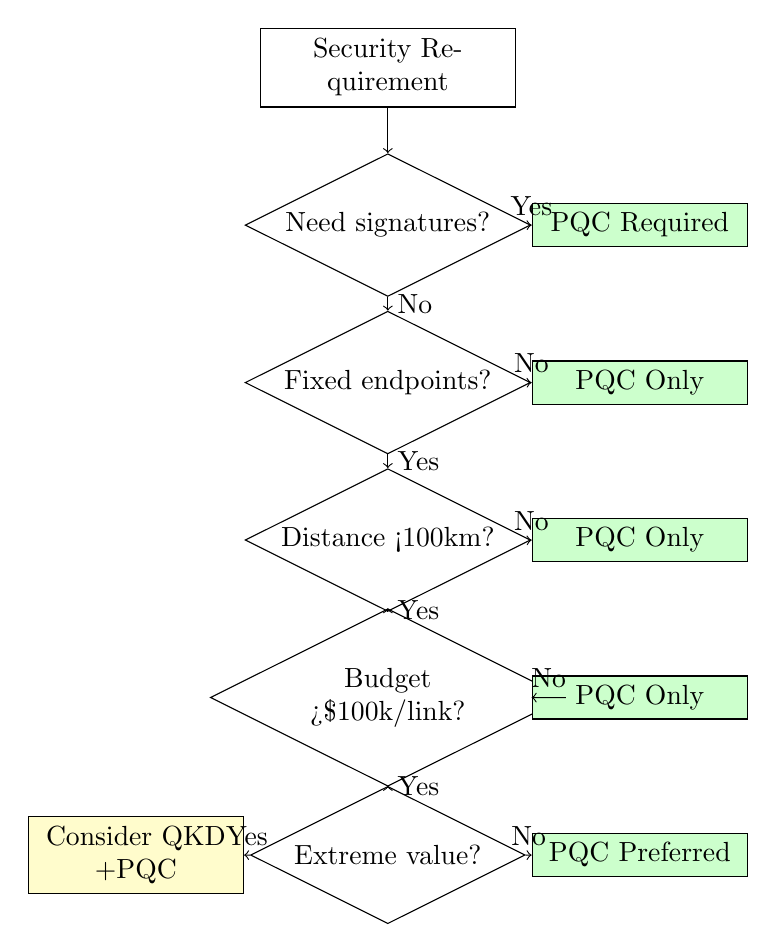
\begin{tikzpicture}[
    decision/.style={diamond, draw, aspect=2, inner sep=0pt, text width=3cm, align=center},
    block/.style={rectangle, draw, text width=3cm, align=center, minimum height=1cm},
    outcome/.style={rectangle, draw, fill=green!20, text width=2.5cm, align=center},
    scale=0.8
]
    % Start
    \node[block] (start) at (0,0) {Security Requirement};
    
    % First decision
    \node[decision] (d1) at (0,-2.5) {Need signatures?};
    \draw[->] (start) -- (d1);
    
    % Signatures needed - PQC only
    \node[outcome] (pqc1) at (4,-2.5) {PQC Required};
    \draw[->] (d1) -- node[above] {Yes} (pqc1);
    
    % No signatures needed
    \node[decision] (d2) at (0,-5) {Fixed endpoints?};
    \draw[->] (d1) -- node[right] {No} (d2);
    
    % Not fixed - PQC
    \node[outcome] (pqc2) at (4,-5) {PQC Only};
    \draw[->] (d2) -- node[above] {No} (pqc2);
    
    % Fixed endpoints
    \node[decision] (d3) at (0,-7.5) {Distance <100km?};
    \draw[->] (d2) -- node[right] {Yes} (d3);
    
    % Too far - PQC
    \node[outcome] (pqc3) at (4,-7.5) {PQC Only};
    \draw[->] (d3) -- node[above] {No} (pqc3);
    
    % Distance OK
    \node[decision] (d4) at (0,-10) {Budget >\$100k/link?};
    \draw[->] (d3) -- node[right] {Yes} (d4);
    
    % No budget - PQC
    \node[outcome] (pqc4) at (4,-10) {PQC Only};
    \draw[->] (d4) -- node[above] {No} (pqc4);
    
    % Has budget
    \node[decision] (d5) at (0,-12.5) {Extreme value?};
    \draw[->] (d4) -- node[right] {Yes} (d5);
    
    % Not extreme - PQC preferred
    \node[outcome] (pqc5) at (4,-12.5) {PQC Preferred};
    \draw[->] (d5) -- node[above] {No} (pqc5);
    
    % Extreme value - Consider QKD
    \node[outcome, fill=yellow!20] (qkd) at (-4,-12.5) {Consider QKD\\+PQC};
    \draw[->] (d5) -- node[above] {Yes} (qkd);
\end{tikzpicture}
\caption{Decision tree: QKD only viable in very specific circumstances}
\end{figure}

\paragraph{Real-World Lessons}

Learning from actual deployments:

\textbf{Successful QKD Deployments:}
\begin{itemize}
    \item \textbf{Geneva election system:} Fixed endpoints, extreme integrity requirements
    \item \textbf{Tokyo QKD network:} R\&D testbed, not production
    \item \textbf{Chinese backbone:} Government resources, national priority
    \item Common factors: Fixed infrastructure, unlimited budget, specific threats
\end{itemize}

\textbf{Failed QKD Projects:}
\begin{itemize}
    \item \textbf{European SECOQC:} Too expensive to maintain after research funding ended
    \item \textbf{Various bank trials:} No advantage over PQC for actual operations
    \item \textbf{Corporate deployments:} Complexity exceeded IT capabilities
    \item Common factors: Underestimated operational costs, overestimated threats
\end{itemize}

\textbf{PQC Migration Experiences:}
\begin{itemize}
    \item \textbf{Google's CECPQ2:} Successfully tested PQC in Chrome with 0.3\% overhead
    \item \textbf{Cloudflare:} Deployed PQC to millions of websites transparently
    \item \textbf{Signal Protocol:} Added PQC with no user-visible changes
    \item Common factors: Software-only deployment, incremental rollout, backward compatible
\end{itemize}

\paragraph{The Practical Reality}

Let's summarize with brutal honesty:

\begin{table}[h]
\centering
\begin{tabular}{|l|c|c|}
\hline
\textbf{Application Category} & \textbf{QKD Viable?} & \textbf{PQC Required?} \\
\hline
Web browsing (HTTPS) & No & Yes \\
Email encryption & No & Yes \\
Software signing & No & Yes \\
VPN/Remote access & No & Yes \\
Cloud services & No & Yes \\
IoT devices & No & Yes \\
Blockchain/Crypto & No & Yes \\
Mobile apps & No & Yes \\
Government backbone & Maybe & Yes \\
Banking backbone & Maybe & Yes \\
Critical infrastructure & Maybe & Yes \\
Diplomatic cables & Yes & Yes \\
\hline
\textbf{Percentage of use cases} & \textbf{<0.1\%} & \textbf{100\%} \\
\hline
\end{tabular}
\caption{The stark reality: PQC is mandatory everywhere, QKD is optional in rare cases}
\end{table}

\begin{remark}[The Bottom Line]
If you're asking "Should I use QKD or PQC?"---you need PQC. The question is whether you \emph{also} need QKD for specific high-value links. For 99.9\% of organizations, PQC alone provides excellent quantum-safe security. QKD is for the 0.1\% with nation-state adversaries, unlimited budgets, and fixed infrastructure. Even then, you still need PQC for signatures.
\end{remark}

This analysis leads naturally to our next topic: how to combine both technologies when extreme security demands it.

\subsubsection{Hybrid Approaches}

Security professionals have a saying: "Defense in depth is the only defense." When protecting against quantum threats, combining QKD and PQC creates multiple independent security layers. If one fails---whether through algorithmic breakthrough, implementation flaw, or operational error---the other maintains protection. This belt-and-suspenders approach makes particular sense during the transition period when we're uncertain about both quantum computer timelines and PQC algorithm security.

\paragraph{Defense in Depth Strategy}

The hybrid philosophy is simple: force an attacker to break multiple, fundamentally different security mechanisms:

\begin{definition}[Hybrid Quantum-Safe Security]
Combine information-theoretic (QKD) and computational (PQC) security such that:
\begin{itemize}
    \item Breaking the system requires breaking BOTH QKD AND PQC
    \item Different expertise needed: quantum physics vs. mathematics/algorithms
    \item Different attack vectors: physical channel vs. computational resources
    \item Failure modes are independent
\end{itemize}
\end{definition}

\begin{figure}[h]
\centering
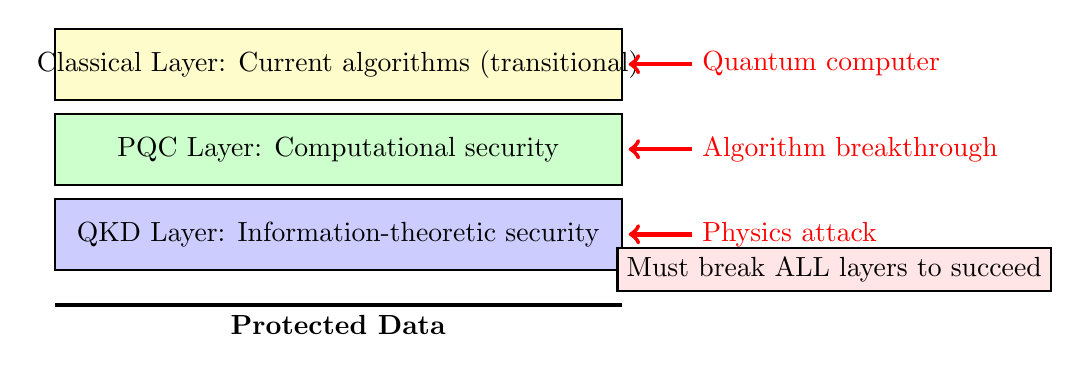
\begin{tikzpicture}[scale=0.9]
    % Security layers
    \draw[thick, fill=blue!20] (0,0) rectangle (8,1);
    \node at (4,0.5) {QKD Layer: Information-theoretic security};
    
    \draw[thick, fill=green!20] (0,1.2) rectangle (8,2.2);
    \node at (4,1.7) {PQC Layer: Computational security};
    
    \draw[thick, fill=yellow!20] (0,2.4) rectangle (8,3.4);
    \node at (4,2.9) {Classical Layer: Current algorithms (transitional)};
    
    % Attack arrows
    \draw[->, ultra thick, red] (9,0.5) -- (8.1,0.5);
    \node[right, red] at (9,0.5) {Physics attack};
    
    \draw[->, ultra thick, red] (9,1.7) -- (8.1,1.7);
    \node[right, red] at (9,1.7) {Algorithm breakthrough};
    
    \draw[->, ultra thick, red] (9,2.9) -- (8.1,2.9);
    \node[right, red] at (9,2.9) {Quantum computer};
    
    % Bottom line
    \draw[ultra thick] (0,-0.5) -- (8,-0.5);
    \node[below] at (4,-0.5) {\textbf{Protected Data}};
    
    % Success requirement
    \node[draw, thick, fill=red!10] at (11,0) {Must break ALL layers to succeed};
\end{tikzpicture}
\caption{Defense in depth: Multiple independent security layers}
\end{figure}

Why this works:
\begin{itemize}
    \item \textbf{QKD break requires:} Violating quantum mechanics or compromising every relay node
    \item \textbf{PQC break requires:} New mathematical algorithm or massive computation
    \item \textbf{Joint break probability:} $P(\text{QKD break}) \times P(\text{PQC break}) \ll$ either alone
    \item \textbf{Diverse expertise:} Few adversaries excel at both quantum physics and advanced mathematics
\end{itemize}

\paragraph{Hybrid Key Establishment}

The core protocol combines QKD and PQC key exchange:

\begin{algorithm}
\caption{Hybrid QKD-PQC Key Establishment}
\label{alg:hybrid-key}
\begin{algorithmic}[1]
\Require QKD link between Alice and Bob
\Require PQC algorithms (e.g., Kyber for KEM, Dilithium for signatures)
\Ensure Shared secret key $K_{\text{final}}$ secure against both quantum and algorithmic attacks

\State \textbf{Phase 1: Authentication}
\State Alice $\rightarrow$ Bob: $\text{Cert}_A$ with PQC public key
\State Bob $\rightarrow$ Alice: $\text{Cert}_B$ with PQC public key
\State Both verify certificates using PQC signatures

\State \textbf{Phase 2: PQC Key Exchange}
\State Bob generates $(pk_{\text{kem}}, sk_{\text{kem}}) \leftarrow \text{Kyber.KeyGen}()$
\State Bob $\rightarrow$ Alice: $pk_{\text{kem}}$, $\text{Sign}_{\text{Dilithium}}(pk_{\text{kem}}, sk_B)$
\State Alice: $(c, K_{\text{PQC}}) \leftarrow \text{Kyber.Encaps}(pk_{\text{kem}})$
\State Alice $\rightarrow$ Bob: $c$, $\text{Sign}_{\text{Dilithium}}(c, sk_A)$
\State Bob: $K_{\text{PQC}} \leftarrow \text{Kyber.Decaps}(c, sk_{\text{kem}})$

\State \textbf{Phase 3: QKD Key Distribution}
\State Run QKD protocol authenticated with $K_{\text{PQC}}$
\State Obtain $K_{\text{QKD}}$ with information-theoretic security

\State \textbf{Phase 4: Key Combination}
\State $K_{\text{final}} = \text{KDF}(K_{\text{QKD}} || K_{\text{PQC}} || \text{transcript})$
\State Both parties have $K_{\text{final}}$ secure against all known attacks
\end{algorithmic}
\end{algorithm}

Key combination methods:

\begin{enumerate}
    \item \textbf{XOR Combination:} $K_{\text{final}} = K_{\text{QKD}} \oplus K_{\text{PQC}}$
    \begin{itemize}
        \item Pro: Provably secure if either key is random
        \item Con: Requires equal-length keys
    \end{itemize}
    
    \item \textbf{KDF Combination:} $K_{\text{final}} = \text{HKDF}(K_{\text{QKD}} || K_{\text{PQC}})$
    \begin{itemize}
        \item Pro: Flexible output length
        \item Pro: Includes context binding
        \item Standard: NIST SP 800-56C
    \end{itemize}
    
    \item \textbf{Dual-Key Usage:} Use different keys for different purposes
    \begin{itemize}
        \item $K_{\text{QKD}}$ for bulk data encryption
        \item $K_{\text{PQC}}$ for authentication/integrity
    \end{itemize}
\end{enumerate}

\paragraph{Authentication Chains}

The circular dependency problem has an elegant solution:

\begin{figure}[h]
\centering
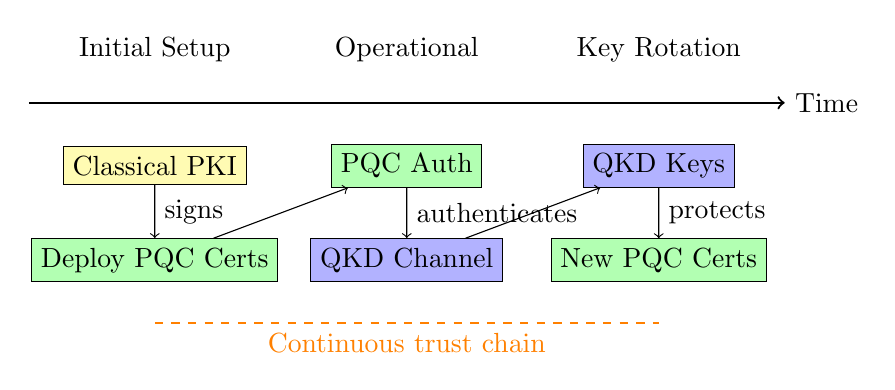
\begin{tikzpicture}[scale=0.8]
    % Time periods
    \draw[thick,->] (0,0) -- (12,0) node[right] {Time};
    \node[above] at (2,0.5) {Initial Setup};
    \node[above] at (6,0.5) {Operational};
    \node[above] at (10,0.5) {Key Rotation};
    
    % Initial auth
    \node[draw, fill=yellow!30] (classic) at (2,-1) {Classical PKI};
    \node[draw, fill=green!30] (pqc) at (2,-2.5) {Deploy PQC Certs};
    \draw[->] (classic) -- (pqc) node[midway,right] {signs};
    
    % Operational phase
    \node[draw, fill=green!30] (pqcauth) at (6,-1) {PQC Auth};
    \node[draw, fill=blue!30] (qkd) at (6,-2.5) {QKD Channel};
    \draw[->] (pqcauth) -- (qkd) node[midway,right] {authenticates};
    \draw[->] (pqc) -- (pqcauth);
    
    % Key rotation
    \node[draw, fill=blue!30] (qkdkeys) at (10,-1) {QKD Keys};
    \node[draw, fill=green!30] (newpqc) at (10,-2.5) {New PQC Certs};
    \draw[->] (qkdkeys) -- (newpqc) node[midway,right] {protects};
    \draw[->] (qkd) -- (qkdkeys);
    
    % Trust flow
    \draw[thick, dashed, orange] (2,-3.5) -- (10,-3.5);
    \node[below, orange] at (6,-3.5) {Continuous trust chain};
\end{tikzpicture}
\caption{Bootstrapping trust: From classical to hybrid quantum-safe}
\end{figure}

This creates a trust ratchet:
\begin{enumerate}
    \item Classical PKI bootstraps initial PQC certificates
    \item PQC certificates authenticate QKD channels
    \item QKD channels protect PQC key distribution
    \item New PQC keys distributed via QKD-secured channels
    \item System never depends solely on classical crypto after bootstrap
\end{enumerate}

\paragraph{Practical Deployment Architectures}

Real-world hybrid deployments use tiered architectures:

\begin{figure}[h]
\centering
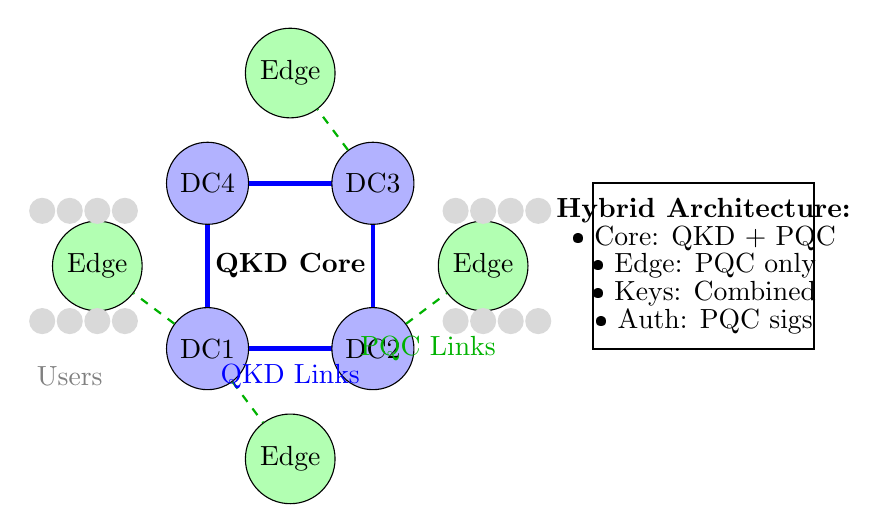
\begin{tikzpicture}[scale=0.7]
    % Core backbone
    \draw[ultra thick, blue] (0,0) -- (3,0) -- (3,3) -- (0,3) -- cycle;
    \node at (1.5,1.5) {\textbf{QKD Core}};
    \node[draw, circle, fill=blue!30] (n1) at (0,0) {DC1};
    \node[draw, circle, fill=blue!30] (n2) at (3,0) {DC2};
    \node[draw, circle, fill=blue!30] (n3) at (3,3) {DC3};
    \node[draw, circle, fill=blue!30] (n4) at (0,3) {DC4};
    
    % QKD links
    \draw[thick, blue] (n1) -- (n2);
    \draw[thick, blue] (n2) -- (n3);
    \draw[thick, blue] (n3) -- (n4);
    \draw[thick, blue] (n4) -- (n1);
    
    % PQC edge
    \node[draw, circle, fill=green!30] (e1) at (-2,1.5) {Edge};
    \node[draw, circle, fill=green!30] (e2) at (5,1.5) {Edge};
    \node[draw, circle, fill=green!30] (e3) at (1.5,-2) {Edge};
    \node[draw, circle, fill=green!30] (e4) at (1.5,5) {Edge};
    
    \draw[thick, green!70!black, dashed] (n1) -- (e1);
    \draw[thick, green!70!black, dashed] (n2) -- (e2);
    \draw[thick, green!70!black, dashed] (n1) -- (e3);
    \draw[thick, green!70!black, dashed] (n3) -- (e4);
    
    % End users
    \foreach \x in {-3,-2.5,-2,-1.5} {
        \node[circle, fill=gray!30] at (\x,0.5) {};
        \node[circle, fill=gray!30] at (\x,2.5) {};
    }
    \foreach \x in {4.5,5,5.5,6} {
        \node[circle, fill=gray!30] at (\x,0.5) {};
        \node[circle, fill=gray!30] at (\x,2.5) {};
    }
    
    % Labels
    \node[blue] at (1.5,-0.5) {QKD Links};
    \node[green!70!black] at (4,0) {PQC Links};
    \node[gray] at (-2.5,-0.5) {Users};
    
    % Legend box
    \draw[thick] (7,0) rectangle (11,3);
    \node[align=left] at (9,2.5) {\textbf{Hybrid Architecture:}};
    \node[align=left] at (9,2) {• Core: QKD + PQC};
    \node[align=left] at (9,1.5) {• Edge: PQC only};
    \node[align=left] at (9,1) {• Keys: Combined};
    \node[align=left] at (9,0.5) {• Auth: PQC sigs};
\end{tikzpicture}
\caption{Typical hybrid deployment: QKD backbone with PQC everywhere}
\end{figure}

\begin{example}[Financial Sector Hybrid Architecture]
Major bank implementing quantum-safe infrastructure:

\textbf{Tier 1 - Critical Core (QKD + PQC):}
\begin{itemize}
    \item Links: Between main data centers
    \item Purpose: Core banking systems, key management
    \item Protection: QKD for key distribution + PQC for authentication
    \item Cost: \$5M for 4 sites
\end{itemize}

\textbf{Tier 2 - Extended Core (PQC only):}
\begin{itemize}
    \item Links: Branch offices, disaster recovery sites
    \item Purpose: Transaction processing, backups
    \item Protection: PQC algorithms (Kyber + Dilithium)
    \item Cost: \$100k for software upgrades
\end{itemize}

\textbf{Tier 3 - Customer Access (PQC only):}
\begin{itemize}
    \item Links: Mobile apps, web banking
    \item Purpose: Customer transactions
    \item Protection: Hybrid classical-PQC during transition
    \item Cost: Included in normal development
\end{itemize}
\end{example}

\paragraph{Migration Strategies}

The path to quantum-safe security isn't binary:

\begin{algorithm}
\caption{Phased Hybrid Migration}
\begin{algorithmic}[1]
\State \textbf{Phase 1: Inventory and Planning} (Now - 2025)
\State \quad Identify all cryptographic dependencies
\State \quad Classify by risk and lifetime
\State \quad Design target architecture

\State \textbf{Phase 2: PQC Foundation} (2025-2027)
\State \quad Deploy PQC alongside classical algorithms
\State \quad $K = \text{KDF}(K_{\text{classical}} || K_{\text{PQC}})$
\State \quad Test performance and compatibility

\State \textbf{Phase 3: QKD Pilots} (2026-2028)
\State \quad Install QKD for highest-value links
\State \quad Integrate with PQC authentication
\State \quad Measure operational costs

\State \textbf{Phase 4: Full Hybrid} (2027-2030)
\State \quad QKD backbone operational
\State \quad PQC mandatory for all systems
\State \quad Classical crypto in compatibility mode only

\State \textbf{Phase 5: Quantum-Safe Only} (2030+)
\State \quad Disable classical algorithms
\State \quad QKD + PQC for critical systems
\State \quad PQC only for general use
\end{algorithmic}
\end{algorithm}

\paragraph{Future-Proofing Through Diversity}

Hybrid approaches provide insurance against multiple failure modes:

\begin{table}[h]
\centering
\begin{tabular}{|l|c|c|c|}
\hline
\textbf{Threat Scenario} & \textbf{Classical} & \textbf{PQC Only} & \textbf{Hybrid} \\
\hline
Quantum computer arrives & Broken & Secure & Secure \\
PQC algorithm broken & Broken$^*$ & Broken & Secure \\
Implementation flaw & Vulnerable & Vulnerable & Partially secure \\
Physical compromise & Secure & Secure & Degraded \\
Zero-day in protocol & Vulnerable & Vulnerable & Partially secure \\
\hline
\multicolumn{4}{l}{$^*$During transition period where both are used}
\end{tabular}
\caption{Hybrid approach provides maximum resilience}
\end{table}

\begin{remark}[Crypto-Agility is Key]
The hybrid approach's greatest benefit isn't the current security—it's the \emph{agility} to respond to future threats:
\begin{itemize}
    \item New quantum algorithm breaks PQC? QKD maintains security
    \item Physical attack on QKD? PQC maintains security  
    \item Better PQC algorithm developed? Deploy without disrupting QKD
    \item Improved QKD technology? Upgrade without changing PQC
\end{itemize}
This agility is worth more than any specific algorithm choice.
\end{remark}

\paragraph{The Realistic Bottom Line}

Hybrid QKD-PQC deployments make sense for:
\begin{itemize}
    \item Organizations with nation-state adversaries
    \item Infrastructure protecting millions of people
    \item Secrets requiring 30+ year protection
    \item Scenarios where trust in any single approach is insufficient
\end{itemize}

For everyone else, PQC alone provides excellent quantum resistance at reasonable cost.

\begin{example}[Decision Matrix]
\begin{center}
\begin{tabular}{|l|l|l|}
\hline
\textbf{Organization Type} & \textbf{Recommendation} & \textbf{Rationale} \\
\hline
Intelligence agency & QKD + PQC hybrid & Maximum adversary capability \\
Major bank (core) & QKD + PQC hybrid & Systemic risk, fixed infrastructure \\
Major bank (branches) & PQC only & Cost-benefit doesn't justify QKD \\
Healthcare system & PQC only & Long-term privacy, but not extreme \\
Enterprise & PQC only & Standard threat model \\
Small business & PQC only & Resource constraints \\
\hline
\end{tabular}
\end{center}
\end{example}

The hybrid approach represents the ultimate in quantum-safe security, but comes with corresponding complexity and cost. For the few organizations that need it, the investment provides unparalleled protection. For everyone else, well-implemented PQC offers quantum safety without the quantum physics.

\subsection{PQC Algorithm Families Overview}
\label{sec:pqc-families}

\subsubsection{Lattice-Based Cryptography}

Here's a stunning fact: when the dust settled on NIST's post-quantum competition, three of the four selected algorithms were based on lattices. Not codes, not hashes, not multivariate polynomials—lattices. This mathematical structure, familiar to every physicist from crystallography and solid-state physics, has emerged as the dominant foundation for post-quantum cryptography. The reasons are compelling: lattices provide efficient algorithms for both encryption and signatures, enable advanced protocols like fully homomorphic encryption, and have resisted cryptanalysis for over 25 years.

\paragraph{Basic Concept: Physics Meets Cryptography}

A lattice is simply all integer linear combinations of basis vectors—a concept physicists encounter daily:

\begin{definition}[Lattice (Informal)]
Given linearly independent vectors $\mathbf{b}_1, ..., \mathbf{b}_n \in \mathbb{R}^n$, the lattice is:
$$\mathcal{L} = \left\{ \sum_{i=1}^n a_i \mathbf{b}_i : a_i \in \mathbb{Z} \right\}$$
\end{definition}

\begin{figure}[h]
\centering
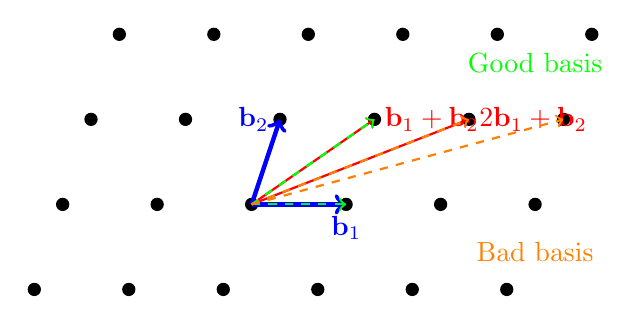
\begin{tikzpicture}[scale=1.2]
    % Draw lattice points
    \foreach \i in {-2,-1,0,1,2,3} {
        \foreach \j in {-1,0,1,2} {
            \pgfmathsetmacro\x{\i + 0.3*\j}
            \pgfmathsetmacro\y{0.9*\j}
            \fill (\x,\y) circle (2pt);
        }
    }
    
    % Draw basis vectors
    \draw[->, ultra thick, blue] (0,0) -- (1,0) node[below] {$\mathbf{b}_1$};
    \draw[->, ultra thick, blue] (0,0) -- (0.3,0.9) node[left] {$\mathbf{b}_2$};
    
    % Draw some lattice vectors
    \draw[->, thick, red] (0,0) -- (1.3,0.9) node[right] {$\mathbf{b}_1 + \mathbf{b}_2$};
    \draw[->, thick, red] (0,0) -- (2.3,0.9) node[right] {$2\mathbf{b}_1 + \mathbf{b}_2$};
    
    % Draw good basis
    \draw[->, thick, green, dashed] (0,0) -- (1.3,0.9);
    \draw[->, thick, green, dashed] (0,0) -- (1,0);
    \node[green] at (3,1.5) {Good basis};
    
    % Draw bad basis
    \draw[->, thick, orange, dashed] (0,0) -- (3.3,0.9);
    \draw[->, thick, orange, dashed] (0,0) -- (2.3,0.9);
    \node[orange] at (3,-0.5) {Bad basis};
\end{tikzpicture}
\caption{Same lattice, different bases: Finding the "good" basis from a "bad" one is cryptographically hard}
\end{figure}

For physicists, think of:
\begin{itemize}
    \item \textbf{Crystal structure:} Atoms at lattice points
    \item \textbf{Reciprocal lattice:} Fourier transform preserves lattice structure
    \item \textbf{Brillouin zones:} Fundamental domains in lattice
    \item \textbf{Basis reduction:} Finding primitive unit cell
\end{itemize}

The cryptographic magic: While you understand lattices in 2D or 3D, cryptography uses lattices in 500+ dimensions where geometric intuition fails and problems become exponentially hard.

\paragraph{The Versatility Advantage}

Unlike other post-quantum approaches, lattices enable the complete cryptographic toolkit:

\begin{table}[h]
\centering
\begin{tabular}{|l|c|c|c|c|}
\hline
\textbf{Capability} & \textbf{Lattice} & \textbf{Code} & \textbf{Hash} & \textbf{Multivariate} \\
\hline
Encryption & \checkmark & \checkmark & \xmark & \checkmark \\
Signatures & \checkmark & \xmark & \checkmark & \checkmark \\
Key Exchange & \checkmark & \checkmark & \xmark & \xmark \\
Homomorphic Encryption & \checkmark & \xmark & \xmark & \xmark \\
Zero-Knowledge Proofs & \checkmark & \xmark & \xmark & Limited \\
Identity-Based Crypto & \checkmark & \xmark & \xmark & \xmark \\
\hline
\textbf{NIST Selections} & \textbf{3} & \textbf{0} & \textbf{1} & \textbf{0} \\
\hline
\end{tabular}
\caption{Lattices uniquely provide all cryptographic primitives efficiently}
\end{table}

This versatility isn't accidental—it stems from the rich algebraic structure:
\begin{itemize}
    \item \textbf{Additive structure:} Enables homomorphic properties
    \item \textbf{Noise tolerance:} Small errors don't break the scheme
    \item \textbf{Worst-case hardness:} Average instances as hard as worst instances
    \item \textbf{Quantum resistance:} No periodic structure to exploit
\end{itemize}

\paragraph{Why Lattices Dominate PQC}

The dominance isn't just about capability—it's about practical engineering:

\begin{enumerate}
    \item \textbf{Security Foundation: 25+ Years Strong}
    \begin{itemize}
        \item NTRU proposed in 1996—still unbroken
        \item LWE introduced in 2005—security only strengthened
        \item Extensive cryptanalysis by worldwide community
        \item No quantum algorithm better than classical
    \end{itemize}
    
    \item \textbf{Efficiency: Reasonable Trade-offs}
    \begin{itemize}
        \item Key sizes: 1-10 KB (vs. MB for codes)
        \item Speed: Often faster than RSA at same security
        \item Simple operations: Just integer arithmetic
        \item Parallelizable: Suits modern hardware
    \end{itemize}
    
    \item \textbf{Flexibility: Multiple Constructions}
    \begin{itemize}
        \item Standard lattices: Maximum security confidence
        \item Ideal lattices: Smaller keys via algebra
        \item Module lattices: Balance between security and efficiency
        \item Each suited for different use cases
    \end{itemize}
\end{enumerate}

\begin{remark}[The Goldilocks Zone]
Lattices occupy a "Goldilocks zone" in PQC:
\begin{itemize}
    \item Codes: Ultra-conservative but keys too large (MB)
    \item Multivariate: Efficient but keeps getting broken
    \item Isogenies: Elegant but catastrophically broken (SIKE)
    \item Lattices: Just right—secure, efficient, and versatile
\end{itemize}
\end{remark}

\paragraph{NIST's Lattice Winners}

Three different lattice approaches won for good reasons:

\textbf{1. CRYSTALS-Kyber (Now ML-KEM): The Encryption Champion}
\begin{itemize}
    \item \textbf{Based on:} Module-LWE (Module Learning With Errors)
    \item \textbf{Strengths:} Fast, reasonable key sizes, simple implementation
    \item \textbf{Key sizes:} 800-1,568 bytes (public), 1,632-3,168 bytes (ciphertext)
    \item \textbf{Use case:} General-purpose encryption, TLS key exchange
    \item \textbf{Why chosen:} Best balance of security and performance
\end{itemize}

\textbf{2. CRYSTALS-Dilithium (Now ML-DSA): The Signature Workhorse}
\begin{itemize}
    \item \textbf{Based on:} Module-LWE with Fiat-Shamir
    \item \textbf{Strengths:} Fast signing and verification, reasonable sizes
    \item \textbf{Signature size:} 2,420-4,595 bytes
    \item \textbf{Use case:} General-purpose signatures, certificates
    \item \textbf{Why chosen:} Best overall signature performance
\end{itemize}

\textbf{3. Falcon: The Compact Alternative}
\begin{itemize}
    \item \textbf{Based on:} NTRU lattices with GPV framework
    \item \textbf{Strengths:} Smallest signatures (666-1,280 bytes)
    \item \textbf{Weakness:} Complex implementation, needs floating-point
    \item \textbf{Use case:} Constrained environments, blockchain
    \item \textbf{Why chosen:} Diversity and compact signatures
\end{itemize}

\begin{figure}[h]
\centering
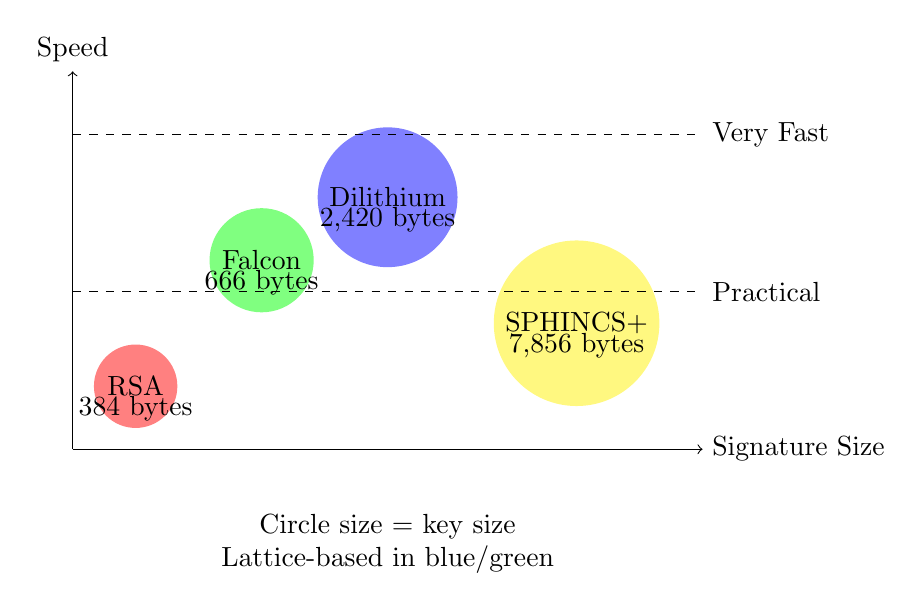
\begin{tikzpicture}[scale=0.8]
    % Axes
    \draw[->] (0,0) -- (10,0) node[right] {Signature Size};
    \draw[->] (0,0) -- (0,6) node[above] {Speed};
    
    % Plot points
    \node[circle, fill=red!50, minimum size=1cm] (rsa) at (1,1) {RSA};
    \node[circle, fill=blue!50, minimum size=1.5cm] (dil) at (5,4) {Dilithium};
    \node[circle, fill=green!50, minimum size=0.8cm] (fal) at (3,3) {Falcon};
    \node[circle, fill=yellow!50, minimum size=2cm] (sph) at (8,2) {SPHINCS+};
    
    % Labels
    \node[below] at (rsa) {384 bytes};
    \node[below] at (dil) {2,420 bytes};
    \node[below] at (fal) {666 bytes};
    \node[below] at (sph) {7,856 bytes};
    
    % Categories
    \draw[dashed] (0,5) -- (10,5) node[right] {Very Fast};
    \draw[dashed] (0,2.5) -- (10,2.5) node[right] {Practical};
    
    % Note
    \node[align=center] at (5,-1.5) {Circle size = key size\\Lattice-based in blue/green};
\end{tikzpicture}
\caption{Performance vs. size trade-offs: Lattice algorithms dominate the practical region}
\end{figure}

\paragraph{Why Three Different Approaches?}

NIST's selection philosophy: diversity protects against catastrophic breaks:

\begin{enumerate}
    \item \textbf{Kyber + Dilithium:} Share Module-LWE foundation
    \begin{itemize}
        \item Pro: Consistent security analysis
        \item Pro: Similar implementation techniques
        \item Risk: Single breakthrough affects both
    \end{itemize}
    
    \item \textbf{Falcon:} Different lattice type (NTRU)
    \begin{itemize}
        \item Pro: Independent security foundation
        \item Pro: Optimal signature sizes
        \item Con: Implementation complexity
    \end{itemize}
    
    \item \textbf{Together:} Cover all use cases
    \begin{itemize}
        \item Need speed? → Dilithium
        \item Need small signatures? → Falcon
        \item Need encryption? → Kyber
        \item Need maximum confidence? → Use hybrid modes
    \end{itemize}
\end{enumerate}

\paragraph{Setting the Stage}

This overview barely scratches the surface. In Section 3, we'll dive deep into:
\begin{itemize}
    \item The mathematics: Why are lattice problems hard?
    \item LWE construction: How noise creates security
    \item Implementation details: From theory to practice
    \item Security analysis: Concrete parameters and attacks
\end{itemize}

\begin{remark}[For the Physics-Minded]
Your crystallography background provides perfect intuition:
\begin{itemize}
    \item Lattice reduction -> Finding primitive unit cell
    \item LWE -> Crystal with thermal noise
    \item Ring-LWE -> Exploiting crystal symmetries
    \item Attacks -> Finding order in apparent disorder
\end{itemize}
The deep dive will make these analogies precise.
\end{remark}

Lattice-based cryptography represents our best hope for a quantum-safe future: versatile enough to replace all current systems, efficient enough for practical deployment, and secure enough to have survived decades of attack. The fact that it connects to physics makes it particularly appealing for this audience—you already have the intuition, we just need to build the cryptographic layer on top.

\subsubsection{Code-Based Cryptography}

If you want the most conservative possible approach to post-quantum cryptography, look no further than code-based systems. The McEliece cryptosystem, proposed in 1978, has survived 45 years of cryptanalysis—longer than RSA, longer than elliptic curves, longer than any other public-key system. It's based on error-correcting codes, a cornerstone of information theory that physicists know from quantum error correction, communication theory, and statistical mechanics. There's just one problem: the keys are enormous.

\paragraph{From Communications to Cryptography}

Error-correcting codes were designed to protect data from noise, not adversaries. The cryptographic insight: decoding a random linear code is NP-complete.

\begin{definition}[The Syndrome Decoding Problem]
Given:
\begin{itemize}
    \item A random binary matrix $H \in \{0,1\}^{r \times n}$ (parity check matrix)
    \item A syndrome $s \in \{0,1\}^r$
    \item An integer $w$ (error weight)
\end{itemize}
Find: An error vector $e \in \{0,1\}^n$ with exactly $w$ ones such that $He^T = s$.
\end{definition}

For physicists, this connects to:
\begin{itemize}
    \item \textbf{Statistical mechanics:} Finding low-energy configurations
    \item \textbf{Quantum error correction:} Syndrome measurements and recovery
    \item \textbf{Information theory:} Channel capacity and decoding limits
    \item \textbf{Compressed sensing:} Sparse signal recovery
\end{itemize}

\begin{figure}[h]
\centering
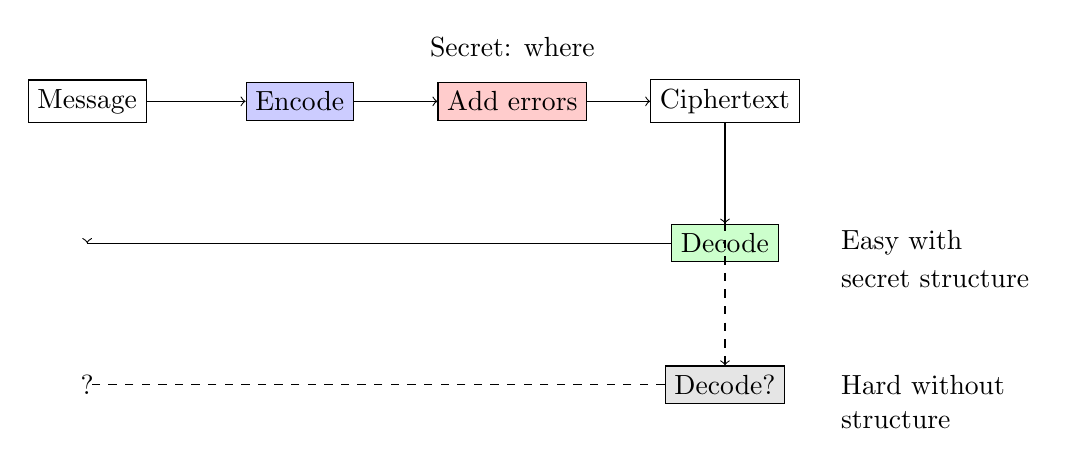
\begin{tikzpicture}[scale=0.9]
    % Original message
    \node[draw, rectangle] (msg) at (0,0) {Message};
    
    % Encoding
    \node[draw, rectangle, fill=blue!20] (enc) at (3,0) {Encode};
    \draw[->] (msg) -- (enc);
    
    % Add errors
    \node[draw, rectangle, fill=red!20] (err) at (6,0) {Add errors};
    \draw[->] (enc) -- (err);
    \node[above] at (6,0.5) {Secret: where};
    
    % Ciphertext
    \node[draw, rectangle] (ct) at (9,0) {Ciphertext};
    \draw[->] (err) -- (ct);
    
    % Legitimate decoding
    \node[draw, rectangle, fill=green!20] (dec1) at (9,-2) {Decode};
    \draw[->] (ct) -- (dec1);
    \node[right] at (10.5,-2) {Easy with};
    \node[right] at (10.5,-2.5) {secret structure};
    
    % Attacker
    \node[draw, rectangle, fill=gray!20] (dec2) at (9,-4) {Decode?};
    \draw[->, dashed] (ct) -- (dec2);
    \node[right] at (10.5,-4) {Hard without};
    \node[right] at (10.5,-4.5) {structure};
    
    % Back to message
    \draw[->] (dec1) -| (0,-2);
    \draw[dashed] (dec2) -| (0,-4);
    \node at (0,-4) {?};
\end{tikzpicture}
\caption{Code-based encryption: Hide efficient decoding structure in random-looking code}
\end{figure}

The cryptographic magic: Use a code with hidden structure that allows efficient decoding, but looks random to attackers.

\paragraph{The McEliece Cryptosystem}

McEliece's 1978 construction remains unbroken—a record unmatched in cryptography:

\begin{algorithm}
\caption{McEliece Encryption (Simplified)}
\begin{algorithmic}[1]
\State \textbf{Key Generation:}
\State \quad Choose a Goppa code with generator matrix $G$
\State \quad Choose random invertible matrices $S$ and $P$
\State \quad Public key: $G' = SGP$ (looks random)
\State \quad Private key: $(S, G, P)$ and Goppa polynomial

\State \textbf{Encryption:}
\State \quad Message: $m \in \{0,1\}^k$
\State \quad Random error: $e \in \{0,1\}^n$ with weight $t$
\State \quad Ciphertext: $c = mG' + e$

\State \textbf{Decryption:}
\State \quad Compute $cP^{-1} = mSG + eP^{-1}$
\State \quad Use Goppa decoding to remove error
\State \quad Recover $m$ by inverting $S$
\end{algorithmic}
\end{algorithm}

Security relies on two problems:
\begin{enumerate}
    \item \textbf{Generic decoding:} Removing unknown errors from random code
    \item \textbf{Distinguishing:} Goppa codes look random after transformation
\end{enumerate}

\begin{example}[Concrete Parameters]
Classic McEliece for 128-bit quantum security:
\begin{itemize}
    \item Code parameters: $[3488, 2720, 129]$ Goppa code
    \item Public key size: 261,120 bytes (255 KB)
    \item Ciphertext expansion: 128 bytes
    \item Private key: 6,492 bytes
    \item Compare RSA-2048: 256 bytes public key
\end{itemize}
\end{example}

\paragraph{Quantum Resistance: Information-Theoretic Near-Optimality}

Code-based cryptography resists quantum attack for fundamental reasons:

\begin{enumerate}
    \item \textbf{No Hidden Structure:} Generic codes have no periodicity or algebra to exploit
    \item \textbf{Grover is Optimal:} Best quantum algorithm is Grover's search
    \item \textbf{Well-Understood Bounds:} Information theory provides tight limits
\end{enumerate}

\begin{theorem}[Quantum Complexity of Syndrome Decoding]
For a random $(n,k)$ code with $t$ errors:
\begin{itemize}
    \item Classical: $\mathcal{O}(2^{kt/n})$ operations
    \item Quantum: $\mathcal{O}(2^{kt/2n})$ operations (Grover speedup)
    \item No exponential quantum advantage known
\end{itemize}
\end{theorem}

\begin{figure}[h]
\centering
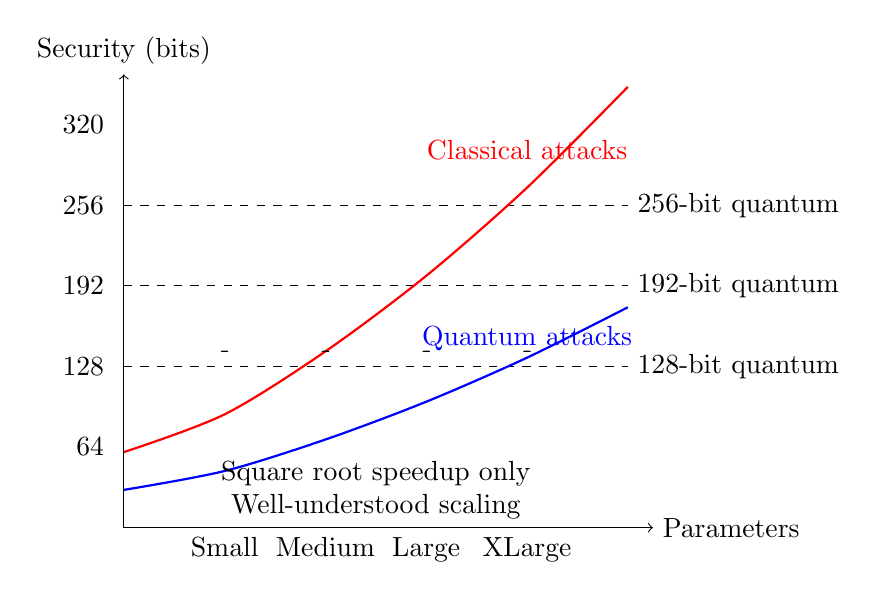
\begin{tikzpicture}[
    scale=0.8,
    % CRITICAL: Scale down y-coordinates
    yscale=0.02,  % This scales 300 units to 6 units visually
    xscale=0.8
]
    % Security level lines
    \draw[dashed] (0,128) -- (10,128) node[right] {128-bit quantum};
    \draw[dashed] (0,192) -- (10,192) node[right] {192-bit quantum};
    \draw[dashed] (0,256) -- (10,256) node[right] {256-bit quantum};
    
    % Classical attacks
    \draw[thick, red] plot[smooth] coordinates {(0,60) (2,90) (4,140) (6,200) (8,270) (10,350)};
    \node[red] at (8,300) {Classical attacks};
    
    % Quantum attacks
    \draw[thick, blue] plot[smooth] coordinates {(0,30) (2,45) (4,70) (6,100) (8,135) (10,175)};
    \node[blue] at (8,150) {Quantum attacks};
    
    % Parameters
    \foreach \x/\params in {2/Small, 4/Medium, 6/Large, 8/XLarge} {
        \draw[fill=black] (\x,140) circle (2pt);
        \node[below] at (\x,0) {\params};
    }
    
    % Axes
    \draw[->] (0,0) -- (10.5,0) node[right] {Parameters};
    \draw[->] (0,0) -- (0,360) node[above] {Security (bits)};
    
    % Y-axis labels (compensate for scaling)
    \foreach \y/\label in {64/64, 128/128, 192/192, 256/256, 320/320} {
        \node[left] at (-0.2,\y) {\label};
    }
    
    % Note
    \node[align=center] at (5,30) {Square root speedup only\\Well-understood scaling};
\end{tikzpicture}
\caption{Code-based security: Quantum provides only Grover speedup}
\end{figure}


\paragraph{The Achilles' Heel: Key Size}

The fatal flaw that prevented NIST selection:

\begin{table}[h]
\centering
\begin{tabular}{|l|r|r|r|}
\hline
\textbf{Algorithm} & \textbf{Public Key} & \textbf{Ciphertext} & \textbf{Security} \\
\hline
RSA-2048 & 256 B & 256 B & 112-bit classical \\
ECDH-P256 & 64 B & 64 B & 128-bit classical \\
\hline
Kyber-768 & 1,184 B & 1,088 B & 128-bit quantum \\
Dilithium-3 & 1,952 B & 3,293 B (sig) & 128-bit quantum \\
\hline
Classic McEliece & \textbf{261,120 B} & 128 B & 128-bit quantum \\
\hline
\end{tabular}
\caption{The key size catastrophe: 1000× larger than current systems}
\end{table}

Why are keys so large?
\begin{itemize}
    \item Need large random matrix to hide structure
    \item Matrix must be dense (not sparse) for security
    \item No algebraic compression possible
    \item Linear in security parameter
\end{itemize}

\begin{example}[Bandwidth Impact]
TLS handshake with Classic McEliece:
\begin{itemize}
    \item Current (ECDH): ~1.5 KB total
    \item With McEliece: ~262 KB total
    \item 175× increase in handshake size
    \item For Google: 30+ petabytes/day extra
\end{itemize}
\end{example}

\paragraph{NIST Competition Results}

Classic McEliece made it to the final round but wasn't selected:

\textbf{Strengths recognized by NIST:}
\begin{itemize}
    \item Longest security track record
    \item Simple security assumption
    \item Fast operations
    \item Small ciphertext expansion
\end{itemize}

\textbf{Why not selected:}
\begin{itemize}
    \item Public keys too large for most applications
    \item Bandwidth costs prohibitive
    \item Storage requirements unrealistic
    \item Lattice schemes offer better trade-offs
\end{itemize}

NIST's comment: "Classic McEliece has unmatched security confidence but deployment challenges make it unsuitable as a general-purpose standard."

\paragraph{The Trade-off Dilemma}

Code-based cryptography presents a stark choice:

\begin{figure}[h]
\centering
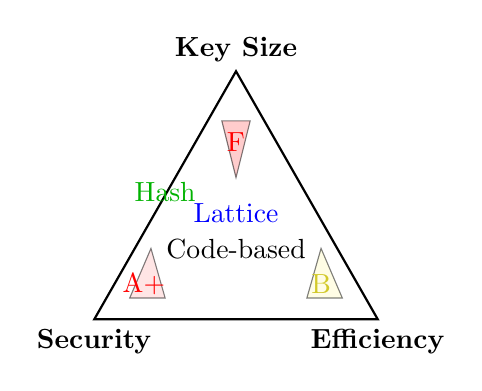
\begin{tikzpicture}[scale=0.9]
    % Triangle
    \draw[thick] (0,0) -- (4,0) -- (2,3.5) -- cycle;
    
    % Vertices
    \node[below] at (0,0) {\textbf{Security}};
    \node[below] at (4,0) {\textbf{Efficiency}};
    \node[above] at (2,3.5) {\textbf{Key Size}};
    
    % Regions
    \node at (2,1) {Code-based};
    \draw[fill=red!20, opacity=0.5] (0.5,0.3) -- (1,0.3) -- (0.8,1) -- cycle;
    \node[red] at (0.7,0.5) {A+};
    
    \draw[fill=yellow!20, opacity=0.5] (3,0.3) -- (3.5,0.3) -- (3.2,1) -- cycle;
    \node[yellow!80!black] at (3.2,0.5) {B};
    
    \draw[fill=red!40, opacity=0.5] (1.8,2.8) -- (2.2,2.8) -- (2,2) -- cycle;
    \node[red] at (2,2.5) {F};
    
    % Other schemes
    \node[blue] at (2,1.5) {Lattice};
    \node[green!70!black] at (1,1.8) {Hash};
\end{tikzpicture}
\caption{The impossible triangle: Code-based crypto excels at security and speed but fails at key size}
\end{figure}

\textbf{Where code-based might still make sense:}
\begin{itemize}
    \item \textbf{High-bandwidth scenarios:} Backbone links with fiber capacity
    \item \textbf{Paranoid security:} When you absolutely cannot risk algorithmic breaks
    \item \textbf{Future storage:} If storage becomes essentially free
    \item \textbf{Hybrid modes:} Combine with lattice for diversity
\end{itemize}

\begin{remark}[The Conservation Law of Cryptography]
Code-based cryptography illustrates a fundamental trade-off: you can have any two of {small keys, high security, computational efficiency}, but not all three. McEliece chose security and efficiency, sacrificing key size. Lattices found a better balance for most applications, but at the cost of newer, less-tested mathematical assumptions. There's no free lunch in post-quantum cryptography.
\end{remark}

\begin{example}[Potential Future: Compressed Codes]
Research continues on reducing key sizes:
\begin{itemize}
    \item Quasi-cyclic codes: Some structure, smaller keys
    \item List decoding: Higher error rates, smaller codes
    \item New code families: Moderate improvements
    \item Reality check: Still 10-100× larger than lattices
\end{itemize}
\end{example}

Code-based cryptography remains the "gold standard" for conservative security—if you can afford the keys. For special applications where bandwidth and storage aren't constraints, it provides unmatched confidence. For everyone else, the key sizes remain prohibitive. As NIST concluded, it's a specialized tool rather than a general solution, but one that provides an important existence proof: we have at least one approach that has survived everything cryptanalysts have thrown at it for nearly half a century.

\subsubsection{Hash-Based Signatures}

Here's a beautiful fact: you can build quantum-secure digital signatures using nothing but hash functions. No number theory, no lattices, no algebraic structures—just the humble one-way function. This minimalist approach offers ultimate confidence: if SHA-256 remains one-way against quantum computers (with appropriate parameter increases), then hash-based signatures remain secure. There's just one catch: this approach \textbf{only} works for signatures, never encryption. SPHINCS+, the hash-based winner in NIST's competition, represents the culmination of 40 years of research into turning this theoretical possibility into practical reality.

\paragraph{Building from One-Way Functions}

The journey starts with Lamport's elegant one-time signature from 1979:

\begin{algorithm}
\caption{Lamport One-Time Signature (Simplified)}
\begin{algorithmic}[1]
\State \textbf{Key Generation:}
\State \quad For each bit position $i = 1$ to $n$:
\State \quad \quad Choose random values $x_i^0, x_i^1 \in \{0,1\}^{256}$
\State \quad \quad Compute $y_i^0 = H(x_i^0)$, $y_i^1 = H(x_i^1)$
\State \quad Private key: $\{x_i^0, x_i^1\}_{i=1}^n$
\State \quad Public key: $\{y_i^0, y_i^1\}_{i=1}^n$

\State \textbf{Sign} message $m = m_1 m_2 ... m_n$:
\State \quad For each bit $m_i$: reveal $x_i^{m_i}$
\State \quad Signature: $(x_1^{m_1}, x_2^{m_2}, ..., x_n^{m_n})$

\State \textbf{Verify} signature $(s_1, ..., s_n)$ on $m$:
\State \quad Check: $H(s_i) = y_i^{m_i}$ for all $i$
\end{algorithmic}
\end{algorithm}

\begin{figure}[h]
\centering
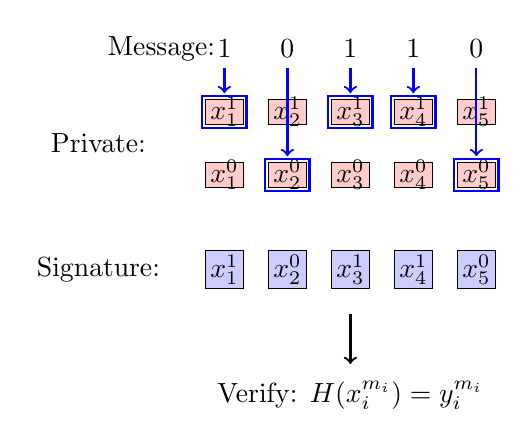
\begin{tikzpicture}[scale=0.8]
    % Message bits
    \node at (-1, 3) {Message:};
    \foreach \i/\bit in {1/1, 2/0, 3/1, 4/1, 5/0} {
        \node at (\i-1, 3) {$\bit$};
    }
    
    % Private key
    \node at (-2, 1.5) {Private:};
    \foreach \i in {1,2,3,4,5} {
        \draw[fill=red!20] (\i-1-0.3, 0.8) rectangle (\i-1+0.3, 1.2);
        \node at (\i-1, 1) {$x_\i^0$};
        \draw[fill=red!20] (\i-1-0.3, 1.8) rectangle (\i-1+0.3, 2.2);
        \node at (\i-1, 2) {$x_\i^1$};
    }
    
    % Signature selection
    \foreach \i/\bit in {1/1, 2/0, 3/1, 4/1, 5/0} {
        \ifnum\bit=1
            \draw[thick, blue, ->] (\i-1, 2.7) -- (\i-1, 2.3);
            \draw[thick, blue] (\i-1-0.35, 1.75) rectangle (\i-1+0.35, 2.25);
        \else
            \draw[thick, blue, ->] (\i-1, 2.7) -- (\i-1, 1.3);
            \draw[thick, blue] (\i-1-0.35, 0.75) rectangle (\i-1+0.35, 1.25);
        \fi
    }
    
    % Signature
    \node at (-2, -0.5) {Signature:};
    \foreach \i/\bit in {1/1, 2/0, 3/1, 4/1, 5/0} {
        \draw[fill=blue!20] (\i-1-0.3, -0.8) rectangle (\i-1+0.3, -0.2);
        \node at (\i-1, -0.5) {$x_\i^\bit$};
    }
    
    % Arrow to public key verification
    \draw[thick, ->] (2, -1.2) -- (2, -2);
    \node at (2, -2.5) {Verify: $H(x_i^{m_i}) = y_i^{m_i}$};
\end{tikzpicture}
\caption{Lamport signatures: Reveal half of the secrets based on message bits}
\end{figure}

Why "one-time"? Signing two different messages reveals different private key pieces, allowing forgery:
\begin{itemize}
    \item Sign $m = 1010...$: Reveals $(x_1^1, x_2^0, x_3^1, x_4^0, ...)$
    \item Sign $m' = 1110...$: Reveals $(x_1^1, x_2^1, x_3^1, x_4^0, ...)$
    \item Attacker knows both $x_2^0$ and $x_2^1$: Can forge bit 2 as either value
\end{itemize}

\paragraph{From One-Time to Many-Time: The Merkle Tree}

Merkle (1979) showed how to sign many messages by organizing one-time keys in a tree:

\begin{figure}[h]
\centering
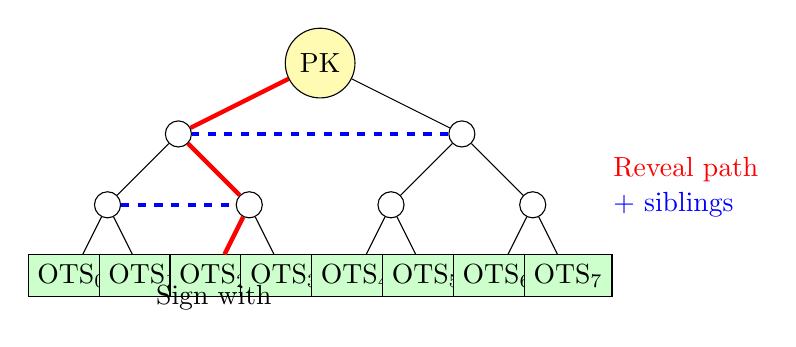
\begin{tikzpicture}[scale=0.9]
    % Level 0 (root)
    \node[circle, draw, fill=yellow!30] (root) at (4,4) {PK};
    
    % Level 1
    \node[circle, draw] (h1) at (2,3) {};
    \node[circle, draw] (h2) at (6,3) {};
    
    % Level 2
    \node[circle, draw] (h11) at (1,2) {};
    \node[circle, draw] (h12) at (3,2) {};
    \node[circle, draw] (h21) at (5,2) {};
    \node[circle, draw] (h22) at (7,2) {};
    
    % Level 3 (leaves - OTS keys)
    \foreach \i in {0,1,2,3,4,5,6,7} {
        \node[rectangle, draw, fill=green!20] (ots\i) at (\i+0.5,1) {$\text{OTS}_\i$};
    }
    
    % Connections
    \draw (root) -- (h1);
    \draw (root) -- (h2);
    \draw (h1) -- (h11);
    \draw (h1) -- (h12);
    \draw (h2) -- (h21);
    \draw (h2) -- (h22);
    \foreach \i in {0,1} {
        \draw (h11) -- (ots\i);
    }
    \foreach \i in {2,3} {
        \draw (h12) -- (ots\i);
    }
    \foreach \i in {4,5} {
        \draw (h21) -- (ots\i);
    }
    \foreach \i in {6,7} {
        \draw (h22) -- (ots\i);
    }
    
    % Authentication path
    \draw[ultra thick, red] (ots2) -- (h12);
    \draw[ultra thick, red] (h12) -- (h1);
    \draw[ultra thick, red] (h1) -- (root);
    \draw[ultra thick, blue, dashed] (h11) -- (h12);
    \draw[ultra thick, blue, dashed] (h2) -- (h1);
    
    % Labels
    \node[below] at (ots2) {Sign with};
    \node[right, red] at (8,2.5) {Reveal path};
    \node[right, blue] at (8,2) {+ siblings};
\end{tikzpicture}
\caption{Merkle tree: One public key authenticates many one-time signatures}
\end{figure}

To sign the $i$-th message:
\begin{enumerate}
    \item Use $\text{OTS}_i$ to sign the message
    \item Reveal authentication path from leaf to root
    \item Verifier reconstructs root, checks against public key
\end{enumerate}

\textbf{The state management nightmare:}
\begin{itemize}
    \item \textbf{Critical:} Never reuse an OTS key
    \item \textbf{Problem:} Must track which keys are used
    \item \textbf{Distributed systems:} State synchronization across nodes
    \item \textbf{Backup/restore:} State loss = security catastrophe
    \item \textbf{Result:} Beautiful in theory, dangerous in practice
\end{itemize}

\paragraph{The Stateless Revolution: SPHINCS+}

SPHINCS+ (2019) eliminates state by using "few-time" signatures and hypertrees:

\begin{definition}[Few-Time Signature]
Instead of one-time signatures that break after two uses, use schemes that tolerate hundreds of uses before security degrades. Combined with massive trees, collision probability becomes negligible.
\end{definition}

\begin{figure}[h]
\centering
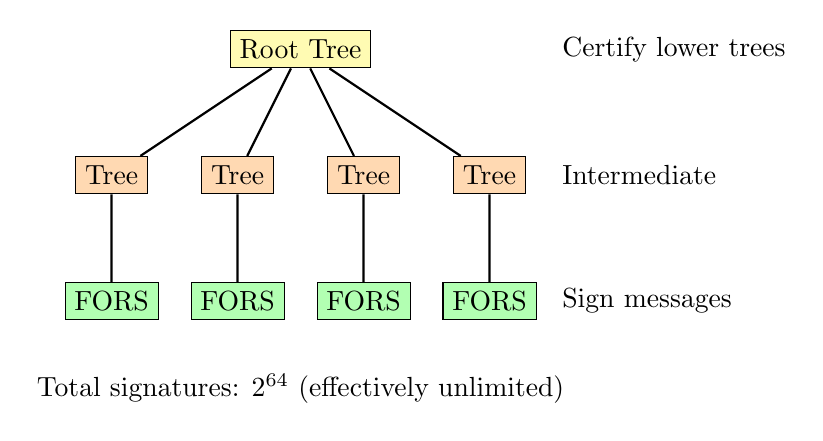
\begin{tikzpicture}[scale=0.8]
    % Hypertree structure
    \node[draw, rectangle, fill=yellow!30] (root) at (4,5) {Root Tree};
    
    % Middle layer
    \node[draw, rectangle, fill=orange!30] (m1) at (1,3) {Tree};
    \node[draw, rectangle, fill=orange!30] (m2) at (3,3) {Tree};
    \node[draw, rectangle, fill=orange!30] (m3) at (5,3) {Tree};
    \node[draw, rectangle, fill=orange!30] (m4) at (7,3) {Tree};
    
    % Bottom layer
    \foreach \i in {1,2,3,4} {
        \node[draw, rectangle, fill=green!30] (b\i) at (2*\i-1,1) {FORS};
    }
    
    % Connections
    \draw[thick] (root) -- (m1);
    \draw[thick] (root) -- (m2);
    \draw[thick] (root) -- (m3);
    \draw[thick] (root) -- (m4);
    \foreach \i in {1,2,3,4} {
        \draw[thick] (m\i) -- (b\i);
    }
    
    % Labels
    \node[right] at (8,5) {Certify lower trees};
    \node[right] at (8,3) {Intermediate};
    \node[right] at (8,1) {Sign messages};
    
    % Parameters
    \node[below] at (4,0) {Total signatures: $2^{64}$ (effectively unlimited)};
\end{tikzpicture}
\caption{SPHINCS+ hypertree: Stateless through massive tree and few-time signatures}
\end{figure}

Key innovations:
\begin{itemize}
    \item \textbf{FORS:} Few-time signatures tolerating many uses
    \item \textbf{Hypertree:} Multiple tree layers for efficiency
    \item \textbf{Randomized signing:} Pseudo-random index selection
    \item \textbf{No state needed:} Deterministic from message + key
\end{itemize}

\paragraph{NIST Selection: The Conservative Backup}

SPHINCS+ was selected as the fourth algorithm for specific reasons:

\begin{table}[h]
\centering
\begin{tabular}{|l|r|r|r|}
\hline
\textbf{Algorithm} & \textbf{Type} & \textbf{Signature Size} & \textbf{Speed} \\
\hline
Dilithium3 & Lattice & 3,293 B & 2,000 sig/sec \\
Falcon-512 & Lattice & 666 B & 5,000 sig/sec \\
SPHINCS+-128f & Hash & 17,088 B & 100 sig/sec \\
SPHINCS+-128s & Hash & 7,856 B & 15 sig/sec \\
\hline
\end{tabular}
\caption{SPHINCS+ trades size and speed for conservative security}
\end{table}

\textbf{Why NIST included SPHINCS+:}
\begin{itemize}
    \item \textbf{Diversity:} Only non-lattice signature scheme
    \item \textbf{Conservative:} Based solely on hash functions
    \item \textbf{Backup plan:} If lattices break, we have an alternative
    \item \textbf{Special use cases:} Firmware updates, root certificates
\end{itemize}

NIST's comment: "SPHINCS+ provides an important hedge against advances in lattice cryptanalysis, despite larger signatures and slower performance."

\paragraph{The Signature-Only Limitation}

Critical point often misunderstood: hash-based techniques \textbf{cannot} provide encryption.

\textbf{Why no encryption?}
\begin{itemize}
    \item \textbf{One-way only:} Hashes can't be inverted for decryption
    \item \textbf{No trapdoor:} Missing the asymmetry needed for public-key encryption
    \item \textbf{Information theoretic:} Signatures destroy information, encryption preserves it
\end{itemize}

\begin{remark}[A Fundamental Divide]
The physics analogy is thermodynamics:
\begin{itemize}
    \item Signatures = Irreversible process (increase entropy)
    \item Encryption = Reversible process (preserve information)
\end{itemize}
Hash functions are computational "heat engines"—great for irreversible signatures, useless for reversible encryption.
\end{remark}

\textbf{Use cases where hash-based excels:}
\begin{enumerate}
    \item \textbf{Firmware signing:} Size less critical, conservative security vital
    \item \textbf{Root certificates:} Sign once, verify millions of times
    \item \textbf{Long-term archives:} Documents valid for 50+ years
    \item \textbf{Blockchain:} Where signature size is less critical than security
    \item \textbf{Emergency backup:} If all lattice schemes catastrophically fail
\end{enumerate}

\begin{example}[SPHINCS+ in Practice]
Software update signing:
\begin{itemize}
    \item Current (RSA-2048): 256-byte signature
    \item SPHINCS+-128s: 7,856-byte signature
    \item Impact: 30× larger, but...
    \item Update size: 100 MB typical
    \item Overhead: 0.008\% (negligible)
    \item Benefit: Quantum-proof based only on SHA-256
\end{itemize}
\end{example}

\paragraph{The Bottom Line}

Hash-based signatures occupy a unique niche:
\begin{itemize}
    \item \textbf{Most conservative:} Security = existence of one-way functions
    \item \textbf{Limited scope:} Signatures only, no encryption
    \item \textbf{Poor performance:} Large and slow
    \item \textbf{Critical role:} Ultimate backup plan
\end{itemize}

Think of SPHINCS+ as cryptographic insurance: you hope never to need it, but if lattice cryptanalysis achieves a breakthrough, hash-based signatures ensure digital signatures don't disappear entirely. For daily use, stick with Dilithium or Falcon. For ultra-critical, long-term signatures where conservative security trumps efficiency, SPHINCS+ provides unmatched confidence.

\begin{remark}[Historical Note]
Lamport and Merkle invented these techniques before RSA! They were considered impractical curiosities for decades. The quantum threat transformed them from academic exercises into our safety net—a reminder that in cryptography, no idea should be dismissed entirely.
\end{remark}

\subsubsection{Other Approaches}

Cryptography has a graveyard filled with brilliant ideas that didn't survive contact with cryptanalysis. For every RSA or AES that stands the test of time, dozens of schemes lie broken and abandoned. The post-quantum landscape is particularly littered with casualties—schemes that looked promising for years before catastrophic breaks emerged. Understanding these failures isn't just historical curiosity; it's essential for recognizing what makes a cryptographic foundation trustworthy. The spectacular collapse of SIKE in 2022 serves as the most recent and dramatic reminder.

\paragraph{Multivariate Polynomials: The Eternal Optimist}

The idea is seductively simple: solving systems of multivariate quadratic equations over finite fields is NP-complete. Why not build cryptography on this?

\begin{definition}[Multivariate Quadratic (MQ) Problem]
Given $m$ quadratic polynomials in $n$ variables over $\mathbb{F}_q$:
$$p_i(x_1, ..., x_n) = \sum_{j \leq k} a_{ijk} x_j x_k + \sum_j b_{ij} x_j + c_i = 0$$
Find: $(x_1, ..., x_n) \in \mathbb{F}_q^n$ satisfying all equations.
\end{definition}

The cryptographic construction:
\begin{itemize}
    \item \textbf{Private key:} Hidden structure making system easy to solve
    \item \textbf{Public key:} Transformed system looking random
    \item \textbf{Problem:} The hidden structure keeps getting exposed
\end{itemize}

\begin{figure}[h]
\centering
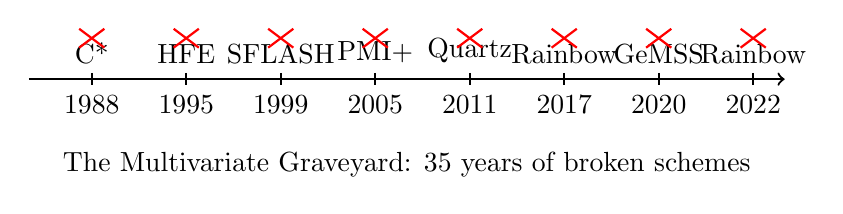
\begin{tikzpicture}[scale=0.8]
    % Timeline of breaks
    \draw[thick, ->] (0,0) -- (12,0);
    
    % Schemes and breaks
    \foreach \x/\year/\name in {1/1988/C*, 2.5/1995/HFE, 4/1999/SFLASH, 5.5/2005/PMI+, 7/2011/Quartz, 8.5/2017/Rainbow, 10/2020/GeMSS, 11.5/2022/Rainbow} {
        \draw[thick] (\x, 0.1) -- (\x, -0.1);
        \node[above] at (\x, 0.1) {\name};
        \node[below] at (\x, -0.1) {\year};
        \draw[red, thick] (\x-0.2, 0.5) -- (\x+0.2, 0.8);
        \draw[red, thick] (\x+0.2, 0.5) -- (\x-0.2, 0.8);
    }
    
    \node[below] at (6, -1) {The Multivariate Graveyard: 35 years of broken schemes};
\end{tikzpicture}
\caption{Multivariate schemes: A consistent pattern of initial promise followed by cryptanalytic breaks}
\end{figure}

\textbf{Why they keep failing:}
\begin{enumerate}
    \item \textbf{Structure leakage:} Hidden structure needed for efficiency is hard to hide completely
    \item \textbf{Algebraic attacks:} Gröbner basis algorithms keep improving
    \item \textbf{Parameter trap:} Make it secure → huge keys; make keys reasonable → breakable
    \item \textbf{Differential attacks:} Structure often visible through derivatives
\end{enumerate}

\begin{example}[Rainbow's Fall]
Rainbow was a NIST finalist until 2022:
\begin{itemize}
    \item Promise: Small signatures (66 bytes!)
    \item Structure: Layers of oil-vinegar equations
    \item Break: Beullens found a way to peel off layers
    \item Result: All proposed parameters broken
    \item Lesson: 20+ years of study wasn't enough
\end{itemize}
\end{example}

\paragraph{The Isogeny Saga: Beauty and Catastrophe}

Isogeny-based cryptography was the newest, most mathematically sophisticated approach—until it spectacularly imploded.

\begin{definition}[Isogenies (Simplified)]
An isogeny is a structure-preserving map between elliptic curves. The cryptographic idea:
\begin{itemize}
    \item Start with elliptic curve $E_0$
    \item Secret: A path through the isogeny graph
    \item Public: The ending curve $E_A$
    \item Hard problem: Find the path from $E_0$ to $E_A$
\end{itemize}
\end{definition}

\begin{figure}[h]
\centering
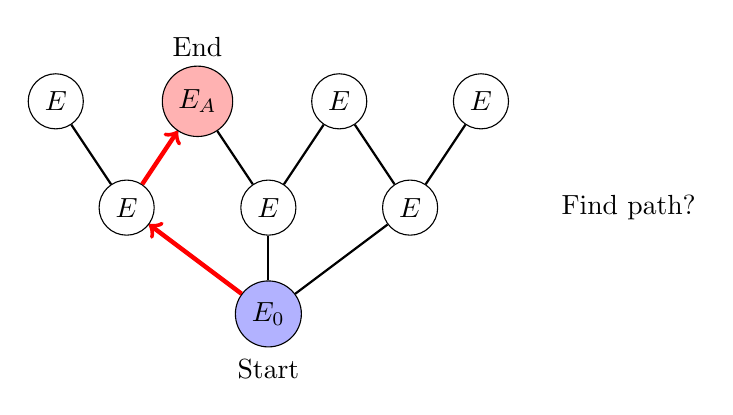
\begin{tikzpicture}[scale=0.9]
    % Isogeny graph
    \node[circle, draw, fill=blue!30] (E0) at (0,0) {$E_0$};
    
    % Level 1
    \node[circle, draw] (E11) at (-2,1.5) {$E$};
    \node[circle, draw] (E12) at (0,1.5) {$E$};
    \node[circle, draw] (E13) at (2,1.5) {$E$};
    
    % Level 2
    \node[circle, draw] (E21) at (-3,3) {$E$};
    \node[circle, draw, fill=red!30] (EA) at (-1,3) {$E_A$};
    \node[circle, draw] (E23) at (1,3) {$E$};
    \node[circle, draw] (E24) at (3,3) {$E$};
    
    % Edges
    \draw[thick] (E0) -- (E11);
    \draw[thick] (E0) -- (E12);
    \draw[thick] (E0) -- (E13);
    \draw[thick] (E11) -- (E21);
    \draw[thick] (E11) -- (EA);
    \draw[thick] (E12) -- (EA);
    \draw[thick] (E12) -- (E23);
    \draw[thick] (E13) -- (E23);
    \draw[thick] (E13) -- (E24);
    
    % Secret path
    \draw[ultra thick, red, ->] (E0) -- (E11);
    \draw[ultra thick, red, ->] (E11) -- (EA);
    
    \node[right] at (4,1.5) {Find path?};
    \node[below] at (0,-0.5) {Start};
    \node[above] at (-1,3.5) {End};
\end{tikzpicture}
\caption{Isogeny graph: Beautiful mathematics, fatal flaw}
\end{figure}

\textbf{SIKE (Supersingular Isogeny Key Encapsulation):}
\begin{itemize}
    \item Submitted to NIST in 2017
    \item Made it to Round 4 (finalist)
    \item Smallest keys among all candidates (335 bytes!)
    \item Based on 10+ years of research
    \item July 2022: Destroyed in 1 hour on a laptop
\end{itemize}

\textbf{The Devastating Attack:}

Castryck and Decru's breakthrough:
\begin{enumerate}
    \item Found auxiliary points with special properties
    \item Used Richelot isogenies and abelian surfaces
    \item Converted path-finding to linear algebra
    \item Complexity: Polynomial instead of exponential!
\end{enumerate}

\begin{remark}[The Shock]
The attack was so unexpected that the SIKE team's initial response was disbelief. The attack used mathematics from the 1990s—nothing quantum, nothing fancy. It had been sitting there, waiting to be discovered, the entire time. The cryptographic community was stunned.
\end{remark}

\begin{example}[Timeline of Doom]
\begin{itemize}
    \item July 30, 2022: Attack posted on ePrint
    \item August 1: Attack verified independently
    \item August 5: All SIKE parameters broken
    \item August 8: Attack extended to SIDH
    \item August 15: Microsoft removes SIKE from libraries
    \item Result: 10 years of work destroyed in 2 weeks
\end{itemize}
\end{example}

\paragraph{Other Failed Attempts}

The graveyard extends beyond these:

\textbf{1. Knapsack Cryptography (1978-1982)}
\begin{itemize}
    \item Based on subset sum (NP-complete!)
    \item Broken by Shamir using lattice reduction
    \item Lesson: Worst-case hardness $\neq$ average-case hardness
\end{itemize}

\textbf{2. Braid Group Cryptography (1999-2007)}
\begin{itemize}
    \item Based on word problem in braid groups
    \item Elegant non-commutative structure
    \item Broken by various heuristic attacks
    \item Lesson: Infinite groups don't guarantee security
\end{itemize}

\textbf{3. Polynomial HFE variants (ongoing)}
\begin{itemize}
    \item Hidden Field Equations and variants
    \item Repeatedly patched and re-broken
    \item Current status: Mostly abandoned
\end{itemize}

\paragraph{What Makes a Survivor?}

Patterns emerge from the carnage:

\textbf{Common failure modes:}
\begin{enumerate}
    \item \textbf{Hidden structure too visible:} Cryptanalysis finds the trapdoor
    \item \textbf{Parameter trap:} Secure parameters make scheme impractical
    \item \textbf{Mathematical brittleness:} One insight breaks everything
    \item \textbf{Limited cryptanalysis:} Not enough eyes on the problem
    \item \textbf{Narrow security margin:} Small parameter increases don't help
\end{enumerate}

\textbf{Properties of survivors:}
\begin{enumerate}
    \item \textbf{Simple underlying problem:} Lattices, codes, hashes
    \item \textbf{Multiple independent constructions:} Different ways to use same hardness
    \item \textbf{Graceful degradation:} Attacks reduce security, don't destroy it
    \item \textbf{20+ years of study:} Time tests all things
    \item \textbf{Connection to other areas:} More researchers, more confidence
\end{enumerate}

\begin{table}[h]
\centering
\begin{tabular}{|l|c|c|c|}
\hline
\textbf{Approach} & \textbf{Years Studied} & \textbf{Status} & \textbf{Why} \\
\hline
Lattices & 25+ & Selected & Robust theory \\
Codes & 45+ & Finalist & Key size only \\
Hash & 40+ & Selected & Conservative \\
Multivariate & 35+ & Broken & Structure leaks \\
Isogeny & 10 & Broken & Auxiliary attack \\
Knapsack & 4 & Broken & Lattice reduction \\
\hline
\end{tabular}
\caption{Time is the ultimate cryptanalytic test}
\end{table}

\paragraph{The Innovation Paradox}

Post-quantum cryptography faces a fundamental tension:

\begin{itemize}
    \item \textbf{Need innovation:} Must replace all current public-key crypto
    \item \textbf{Need conservatism:} Can't afford failures in deployment
    \item \textbf{Result:} Stick with well-studied approaches
\end{itemize}

\begin{remark}[The 20-Year Rule]
An informal principle has emerged: don't trust any cryptographic approach with less than 20 years of serious cryptanalysis. This rules out exciting new mathematics but prevents SIKE-style catastrophes. In cryptography, boring is beautiful.
\end{remark}

\textbf{Lessons from the graveyard:}
\begin{enumerate}
    \item \textbf{Mathematical beauty $\neq$ security:} SIKE was gorgeous mathematics
    \item \textbf{NP-completeness is not enough:} Average case matters
    \item \textbf{Structure for efficiency is dangerous:} It's also structure for attacks
    \item \textbf{Novel mathematics needs decades:} No shortcuts to confidence
    \item \textbf{Multiple approaches essential:} Don't put all eggs in one basket
\end{enumerate}

The spectacular failure of SIKE just as NIST was finalizing standards reinforced the conservative choices. Lattices, codes, and hashes may lack the mathematical excitement of isogenies, but they've survived decades of attack. In cryptography, survival is the only metric that matters.

\begin{example}[The SIKE Postmortem]
What went wrong?
\begin{itemize}
    \item Too much focus on quantum attacks
    \item Not enough on classical cryptanalysis
    \item Auxiliary information considered "harmless"
    \item Small community = fewer eyes
    \item Lesson: Quantum-safe must mean classically-safe first!
\end{itemize}
\end{example}

This tour through the cryptographic graveyard explains why NIST chose conservative, well-studied approaches. The next time someone proposes a brilliant new mathematical foundation for post-quantum cryptography, remember SIKE: mathematical elegance is no defense against a clever graduate student with a laptop.

%==================================================

\section{Deep Dive: Lattice Cryptography}
\label{sec:lattices}

\subsection{Mathematical Foundations}
\label{sec:lattice-math}

\subsubsection{What is a Lattice?}

Let's start with what you already know. In crystallography, a lattice describes the periodic arrangement of atoms in a crystal—a discrete set of points with translational symmetry. Cryptographic lattices are exactly the same mathematical object, just in hundreds of dimensions where your geometric intuition breaks down and computational problems become exponentially hard.

\begin{definition}[Lattice]
A lattice $\mathcal{L} \subseteq \mathbb{R}^n$ is the set of all integer linear combinations of linearly independent basis vectors $\mathbf{b}_1, ..., \mathbf{b}_n \in \mathbb{R}^n$:
$$\mathcal{L}(\mathbf{B}) = \left\{ \sum_{i=1}^n a_i \mathbf{b}_i : a_i \in \mathbb{Z} \right\} = \{\mathbf{B}\mathbf{x} : \mathbf{x} \in \mathbb{Z}^n\}$$
where $\mathbf{B} = [\mathbf{b}_1 | ... | \mathbf{b}_n]$ is the basis matrix.
\end{definition}

\paragraph{The Physics Connection You Already Have}

Your crystallography background provides perfect intuition:

\begin{table}[h]
\centering
\begin{tabular}{|l|l|l|}
\hline
\textbf{Crystallography} & \textbf{Cryptographic Lattices} & \textbf{Key Difference} \\
\hline
3D lattice & $n$-dimensional lattice & $n \approx 500-1000$ \\
Primitive unit cell & Good basis & Many possible bases \\
Reciprocal lattice & Dual lattice & Same hardness properties \\
Brillouin zone & Fundamental domain & Voronoi cell \\
Miller indices & Coefficient vector & Integer constraints \\
Bragg peaks & Lattice points & Discrete structure \\
\hline
\end{tabular}
\caption{Your physics intuition translates directly—until dimension explodes}
\end{table}

\begin{example}[From NaCl to Cryptography]
Consider the face-centered cubic lattice of NaCl:
\begin{itemize}
    \item Basis vectors: $\mathbf{a}_1 = (a,0,0)$, $\mathbf{a}_2 = (0,a,0)$, $\mathbf{a}_3 = (0,0,a)$
    \item You can instantly find the nearest atom to any point
    \item Now imagine this in 700 dimensions—suddenly finding nearest points is exponentially hard
    \item This dimension-induced hardness is the foundation of lattice cryptography
\end{itemize}
\end{example}

\begin{figure}[h]
\centering
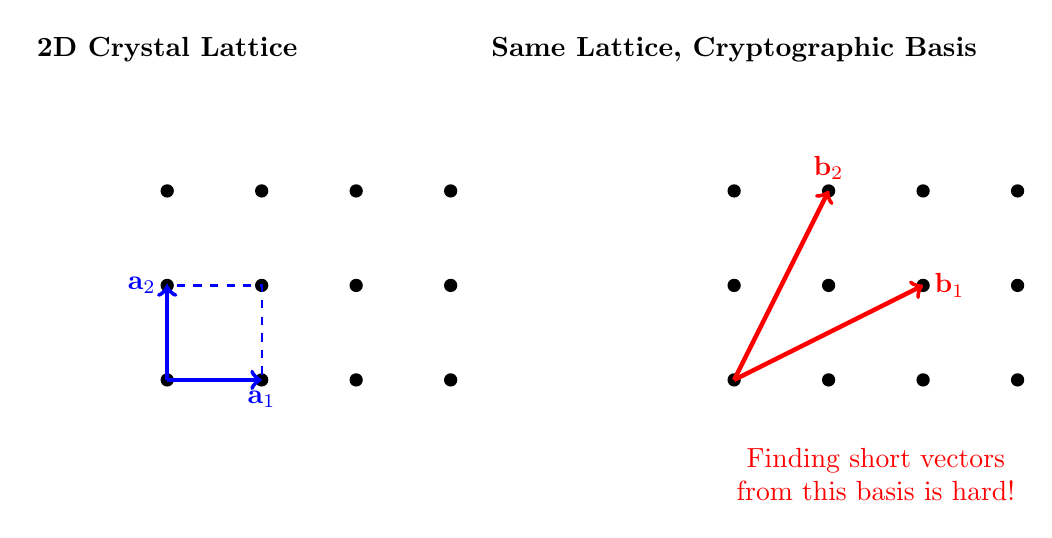
\begin{tikzpicture}[scale=1.2]
    % 2D crystallographic lattice
    \begin{scope}
        \node at (0,3.5) {\textbf{2D Crystal Lattice}};
        % Draw lattice points
        \foreach \i in {0,1,2,3} {
            \foreach \j in {0,1,2} {
                \fill[black] (\i,\j) circle (2pt);
            }
        }
        % Draw basis vectors
        \draw[->, ultra thick, blue] (0,0) -- (1,0) node[below] {$\mathbf{a}_1$};
        \draw[->, ultra thick, blue] (0,0) -- (0,1) node[left] {$\mathbf{a}_2$};
        % Draw unit cell
        \draw[blue, dashed, thick] (0,0) -- (1,0) -- (1,1) -- (0,1) -- cycle;
    \end{scope}
    
    % Cryptographic lattice (skewed)
    \begin{scope}[xshift=6cm]
        \node at (0,3.5) {\textbf{Same Lattice, Cryptographic Basis}};
        % Draw same lattice points
        \foreach \i in {0,1,2,3} {
            \foreach \j in {0,1,2} {
                \fill[black] (\i,\j) circle (2pt);
            }
        }
        % Draw bad basis vectors
        \draw[->, ultra thick, red] (0,0) -- (2,1) node[right] {$\mathbf{b}_1$};
        \draw[->, ultra thick, red] (0,0) -- (1,2) node[above] {$\mathbf{b}_2$};
        % Note about hardness
        \node[red, align=center] at (1.5,-1) {Finding short vectors\\from this basis is hard!};
    \end{scope}
\end{tikzpicture}
\caption{Same lattice points, different bases: The cryptographic challenge}
\end{figure}

\paragraph{Good Basis vs Bad Basis: The Cryptographic Gap}

The same lattice can have exponentially different bases—and this difference creates cryptographic security.

\begin{figure}[h]
\centering
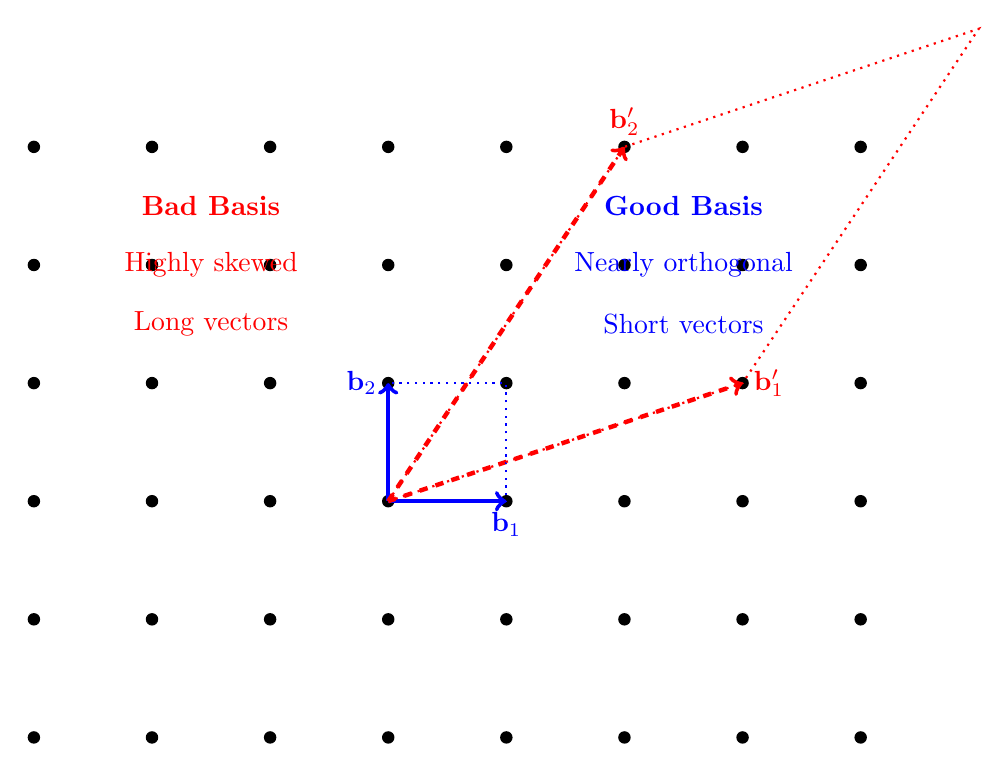
\begin{tikzpicture}[scale=1.5]
    % Grid of lattice points
    \foreach \i in {-3,-2,-1,0,1,2,3,4} {
        \foreach \j in {-2,-1,0,1,2,3} {
            \fill[black] (\i,\j) circle (1.5pt);
        }
    }
    
    % Good basis
    \draw[->, ultra thick, blue] (0,0) -- (1,0) node[below] {$\mathbf{b}_1$};
    \draw[->, ultra thick, blue] (0,0) -- (0,1) node[left] {$\mathbf{b}_2$};
    \node[blue] at (2.5,2.5) {\textbf{Good Basis}};
    \node[blue] at (2.5,2) {Nearly orthogonal};
    \node[blue] at (2.5,1.5) {Short vectors};
    
    % Bad basis
    \draw[->, ultra thick, red, dashed] (0,0) -- (3,1) node[right] {$\mathbf{b}_1'$};
    \draw[->, ultra thick, red, dashed] (0,0) -- (2,3) node[above] {$\mathbf{b}_2'$};
    \node[red] at (-1.5,2.5) {\textbf{Bad Basis}};
    \node[red] at (-1.5,2) {Highly skewed};
    \node[red] at (-1.5,1.5) {Long vectors};
    
    % Fundamental domains
    \draw[blue, thick, dotted] (0,0) -- (1,0) -- (1,1) -- (0,1) -- cycle;
    \draw[red, thick, dotted] (0,0) -- (3,1) -- (5,4) -- (2,3) -- cycle;
\end{tikzpicture}
\caption{Same lattice, vastly different bases: Finding the good basis from the bad is cryptographically hard}
\end{figure}

\begin{example}[Concrete Basis Comparison]
Consider a 2D lattice with two different bases:

\textbf{Good basis:} $\mathbf{B}_{\text{good}} = \begin{pmatrix} 1 & 0 \\ 0 & 1 \end{pmatrix}$
\begin{itemize}
    \item Shortest vector: $(1,0)$ with length 1
    \item Orthogonality defect: 1 (perfect)
    \item Finding short vectors: Trivial
\end{itemize}

\textbf{Bad basis:} $\mathbf{B}_{\text{bad}} = \begin{pmatrix} 97 & 89 \\ 89 & 81 \end{pmatrix}$
\begin{itemize}
    \item Same lattice! (determinant = 1)
    \item Basis vectors have length $>$ 100
    \item Shortest vector still $(1,0)$ but now $= 97\mathbf{b}_1 - 89\mathbf{b}_2$
    \item Finding this combination: Requires sophisticated algorithms
\end{itemize}
\end{example}

\begin{definition}[Basis Quality Measures]
For a basis $\mathbf{B} = [\mathbf{b}_1 | ... | \mathbf{b}_n]$:
\begin{itemize}
    \item \textbf{Orthogonality defect:} $\delta(\mathbf{B}) = \frac{\prod_{i=1}^n \|\mathbf{b}_i\|}{\det(\mathcal{L})}$ (ideal = 1)
    \item \textbf{Hermite factor:} $\gamma = \left(\frac{\|\mathbf{b}_1\|}{\det(\mathcal{L})^{1/n}}\right)^{1/n}$ (smaller = better)
    \item \textbf{Condition number:} $\kappa(\mathbf{B}) = \|\mathbf{B}\| \cdot \|\mathbf{B}^{-1}\|$ (near 1 = good)
\end{itemize}
\end{definition}

\paragraph{The High-Dimensional Reality Check}

Here's where your 3D intuition fails catastrophically:

\begin{theorem}[Dimension Changes Everything]
In dimension $n$:
\begin{enumerate}
    \item Volume of unit ball: $V_n = \frac{\pi^{n/2}}{\Gamma(n/2 + 1)} \to 0$ as $n \to \infty$
    \item Most volume is near the surface: $\frac{V_n(r)}{V_n(R)} = \left(\frac{r}{R}\right)^n$
    \item Random vectors are nearly orthogonal: $\mathbb{E}[|\langle \mathbf{x}, \mathbf{y} \rangle|] = O(1/\sqrt{n})$
    \item Number of "almost shortest" vectors: $\exp(\Theta(n))$
\end{enumerate}
\end{theorem}

\begin{remark}[Why Physicists Should Care]
In condensed matter, you solve lattice problems in 3D constantly—finding ground states, computing band structures, analyzing defects. In 3D, these are polynomial-time problems. In 500D, they become exponentially hard. This dimension-induced phase transition from easy to hard is what protects cryptographic secrets.
\end{remark}

\begin{example}[Concrete Dimension Impact]
Finding shortest vector in random lattice:
\begin{center}
\begin{tabular}{|c|c|c|}
\hline
\textbf{Dimension} & \textbf{Time (best known)} & \textbf{Feasible?} \\
\hline
10 & Seconds & Trivial \\
50 & Hours & Yes \\
100 & Years & Borderline \\
300 & $10^{30}$ years & No \\
700 & $10^{100}$ years & Never \\
\hline
\end{tabular}
\end{center}
Cryptography uses $n \geq 500$ for post-quantum security.
\end{example}

\subsubsection{Fundamental Lattice Problems}

Two problems form the foundation of lattice cryptography. Unlike factoring or discrete log, these problems have resisted efficient algorithms for decades—even with quantum computers.

\paragraph{The Shortest Vector Problem (SVP)}

\begin{definition}[Shortest Vector Problem]
Given a basis $\mathbf{B}$ of lattice $\mathcal{L}$, find a shortest non-zero vector:
$$\mathbf{v} \in \mathcal{L} \setminus \{\mathbf{0}\} \text{ such that } \|\mathbf{v}\| = \lambda_1(\mathcal{L}) = \min_{\mathbf{x} \in \mathcal{L} \setminus \{\mathbf{0}\}} \|\mathbf{x}\|$$
\end{definition}

\begin{figure}[h]
\centering
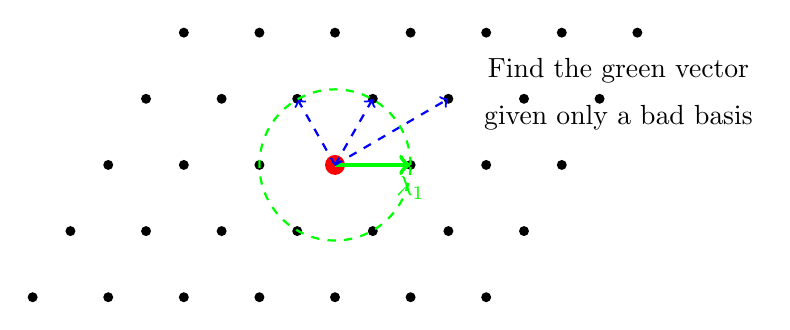
\begin{tikzpicture}[scale=1.2]
    % Lattice points
    \foreach \i in {-3,-2,-1,0,1,2,3} {
        \foreach \j in {-2,-1,0,1,2} {
            \pgfmathsetmacro\x{0.8*\i + 0.4*\j}
            \pgfmathsetmacro\y{0.7*\j}
            \fill[black] (\x,\y) circle (1.5pt);
        }
    }
    
    % Origin
    \fill[red] (0,0) circle (3pt);
    
    % Shortest vector
    \draw[->, ultra thick, green] (0,0) -- (0.8,0) node[below] {$\lambda_1$};
    
    % Some longer vectors
    \draw[->, thick, blue, dashed] (0,0) -- (0.4,0.7);
    \draw[->, thick, blue, dashed] (0,0) -- (1.2,0.7);
    \draw[->, thick, blue, dashed] (0,0) -- (-0.4,0.7);
    
    % Circle showing minimum distance
    \draw[green, thick, dashed] (0,0) circle (0.8);
    
    \node at (3,1) {Find the green vector};
    \node at (3,0.5) {given only a bad basis};
\end{tikzpicture}
\caption{SVP: Find the shortest non-zero lattice vector}
\end{figure}

\textbf{Why SVP is hard:}
\begin{itemize}
    \item \textbf{Exponentially many candidates:} Ball of radius $R$ contains $\approx R^n$ lattice points
    \item \textbf{No local structure:} Can't use gradient descent or similar
    \item \textbf{Discrete geometry:} Continuous relaxations don't help
    \item \textbf{Basis dependence:} Good basis makes it trivial, bad basis makes it hard
\end{itemize}

\paragraph{The Closest Vector Problem (CVP)}

\begin{definition}[Closest Vector Problem]
Given a basis $\mathbf{B}$ of lattice $\mathcal{L}$ and target $\mathbf{t} \in \mathbb{R}^n$, find:
$$\mathbf{v} \in \mathcal{L} \text{ such that } \|\mathbf{v} - \mathbf{t}\| = \min_{\mathbf{x} \in \mathcal{L}} \|\mathbf{x} - \mathbf{t}\|$$
\end{definition}

CVP is the decoding problem: given a noisy codeword, find the original.

\begin{example}[CVP in Cryptography]
In LWE decryption:
\begin{itemize}
    \item Target: $\mathbf{t} = \mathbf{s} + \mathbf{e}$ (secret + small error)
    \item Lattice: Generated by public key
    \item If you can solve CVP: Recover $\mathbf{s}$, break encryption
    \item Reality: CVP is NP-hard even to approximate
\end{itemize}
\end{example}

\paragraph{The Deep Connection: SVP and CVP}

These problems are intimately related through duality:

\begin{theorem}[SVP-CVP Connection]
\begin{enumerate}
    \item CVP in lattice $\mathcal{L}$ $\leftrightarrow$ SVP in modified lattice $\mathcal{L}'$
    \item Solving $\gamma$-CVP gives algorithm for $(2\gamma)$-SVP
    \item Both problems have same quantum complexity (up to polynomial factors)
\end{enumerate}
\end{theorem}

This connection means that progress on one problem immediately impacts the other—a crucial consideration for cryptographic security.

\paragraph{Approximation Variants}

Perfect solutions are often unnecessary. Approximation versions are more relevant:

\begin{definition}[Approximation SVP/CVP]
$\gamma$-SVP: Find $\mathbf{v} \in \mathcal{L}$ with $0 < \|\mathbf{v}\| \leq \gamma \cdot \lambda_1(\mathcal{L})$\\
$\gamma$-CVP: Find $\mathbf{v} \in \mathcal{L}$ with $\|\mathbf{v} - \mathbf{t}\| \leq \gamma \cdot \text{dist}(\mathbf{t}, \mathcal{L})$
\end{definition}

\begin{table}[h]
\centering
\begin{tabular}{|l|c|c|c|}
\hline
\textbf{Approximation Factor} & \textbf{Complexity} & \textbf{Best Algorithm} & \textbf{Quantum?} \\
\hline
$\gamma = 1$ (exact) & NP-hard & Exponential & No speedup \\
$\gamma = O(1)$ & NP-hard & Exponential & No speedup \\
$\gamma = 2^{O(\sqrt{\log n})}$ & Unknown & Sub-exponential & No speedup \\
$\gamma = \text{poly}(n)$ & P (not useful) & Polynomial & Already easy \\
\hline
\end{tabular}
\caption{Hardness depends critically on approximation factor}
\end{table}

\paragraph{The Unique SVP Gap}

Unlike many problems, lattice problems have a "hardness gap":

\begin{theorem}[Hardness Gap for SVP]
For a random lattice $\mathcal{L}$ of dimension $n$:
\begin{itemize}
    \item $\lambda_1(\mathcal{L}) \approx \sqrt{n} \cdot \det(\mathcal{L})^{1/n}$ (shortest vector)
    \item $\lambda_2(\mathcal{L}) \approx \lambda_1(\mathcal{L})$ (second shortest)
    \item But in "planted" lattices: $\lambda_1 \ll \lambda_2$
\end{itemize}
This gap enables cryptographic constructions.
\end{theorem}

\subsubsection{Computational Complexity}

Here's the critical fact that makes lattice cryptography quantum-safe: the best known quantum algorithms for lattice problems offer only polynomial speedups, not exponential ones.

\paragraph{Classical Algorithms: The State of the Art}

\begin{algorithm}
\caption{LLL Algorithm (Simplified)}
\label{alg:lll}
\begin{algorithmic}[1]
\Require Basis $\mathbf{B} = [\mathbf{b}_1, ..., \mathbf{b}_n]$
\Ensure Reduced basis with $\|\mathbf{b}_1\| \leq 2^{(n-1)/2} \lambda_1(\mathcal{L})$
\State $\mathbf{B}^* \gets \text{GramSchmidt}(\mathbf{B})$ \Comment{Orthogonalization}
\State \textbf{repeat}
\State \quad \textbf{for} $i = 2$ to $n$ \textbf{do}
\State \quad \quad \textbf{for} $j = i-1$ down to $1$ \textbf{do}
\State \quad \quad \quad $\mathbf{b}_i \gets \mathbf{b}_i - \lfloor \mu_{i,j} \rceil \mathbf{b}_j$ \Comment{Size reduction}
\State \quad \textbf{for} $i = 1$ to $n-1$ \textbf{do}
\State \quad \quad \textbf{if} Lovász condition violated \textbf{then}
\State \quad \quad \quad Swap $\mathbf{b}_i$ and $\mathbf{b}_{i+1}$
\State \textbf{until} no more swaps
\State \Return $\mathbf{B}$
\end{algorithmic}
\end{algorithm}

\textbf{Algorithm landscape:}
\begin{itemize}
    \item \textbf{LLL (1982):} Polynomial time, exponential approximation
    \item \textbf{BKZ (Block Korkine-Zolotarev):} Time-quality tradeoff
    \item \textbf{Sieving algorithms:} Best for exact SVP
    \item \textbf{Enumeration:} Good for small dimensions
\end{itemize}

\begin{table}[h]
\centering
\begin{tabular}{|l|c|c|c|}
\hline
\textbf{Algorithm} & \textbf{Time} & \textbf{Approximation} & \textbf{Memory} \\
\hline
LLL & $O(n^5 \log B)$ & $2^{O(n)}$ & $O(n^2)$ \\
BKZ-$\beta$ & $2^{O(\beta)}$ & $\gamma^n$, $\gamma = O(\beta/n)$ & $O(n^2)$ \\
Sieving & $2^{0.292n + o(n)}$ & Exact & $2^{0.208n}$ \\
Enumeration & $2^{O(n \log n)}$ & Exact & $\text{poly}(n)$ \\
\hline
\end{tabular}
\caption{Classical algorithms: Trade time for approximation quality}
\end{table}

\paragraph{Quantum (Non-)Advantages}

The quantum story for lattices is remarkably different from factoring:

\begin{theorem}[Quantum Speedup for Lattice Problems]
Best known quantum algorithms for $n$-dimensional lattice problems:
\begin{itemize}
    \item SVP: $2^{0.265n + o(n)}$ (vs classical $2^{0.292n + o(n)}$)
    \item CVP: Similar modest improvement
    \item Speedup: $2^{0.027n} \approx 1.019^n$ (not exponential!)
\end{itemize}
\end{theorem}

\begin{figure}[h]
\centering
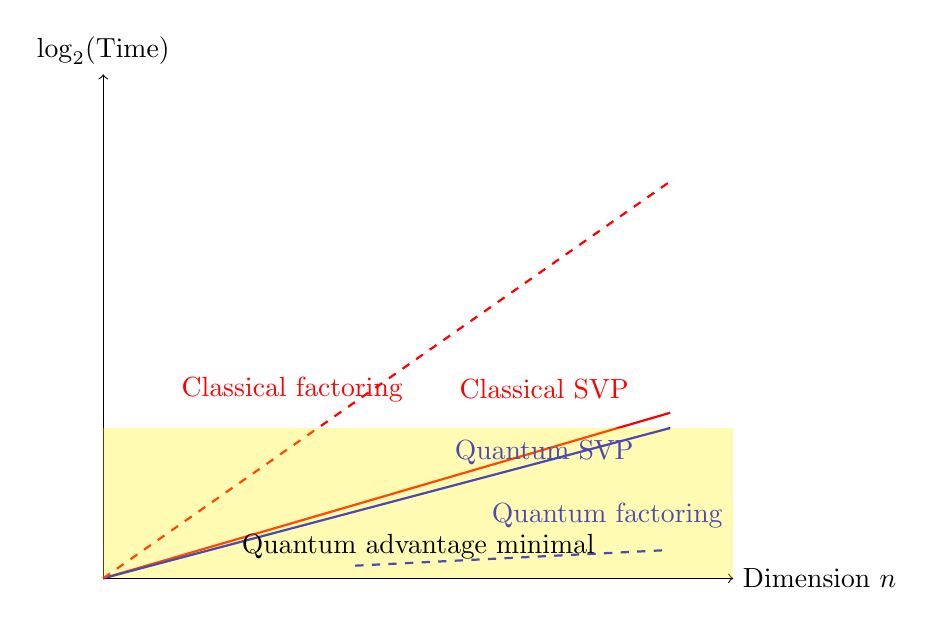
\begin{tikzpicture}[scale=0.8]
    % Axes
    \draw[->] (0,0) -- (10,0) node[right] {Dimension $n$};
    \draw[->] (0,0) -- (0,8) node[above] {$\log_2$(Time)};
    
    % Classical SVP
    \draw[thick, red] plot[domain=0:9] (\x, {0.292*\x});
    \node[red] at (7,3) {Classical SVP};
    
    % Quantum SVP
    \draw[thick, blue] plot[domain=0:9] (\x, {0.265*\x});
    \node[blue] at (7,2) {Quantum SVP};
    
    % Factoring comparison
    \draw[thick, red, dashed] plot[domain=0:9] (\x, {0.7*\x});
    \node[red] at (3,3) {Classical factoring};
    
    \draw[thick, blue, dashed] plot[domain=4:9] (\x, {0.05*\x});
    \node[blue] at (8,1) {Quantum factoring};
    
    % Shaded region
    \fill[yellow, opacity=0.3] (0,0) rectangle (10,0.265*9);
    \node at (5,0.5) {Quantum advantage minimal};
\end{tikzpicture}
\caption{Quantum speedup for lattices is polynomial, not exponential like factoring}
\end{figure}

\textbf{Why no quantum breakthrough?}
\begin{enumerate}
    \item \textbf{No periodic structure:} Shor's algorithm needs periodicity
    \item \textbf{No hidden subgroup:} Lattice problems don't fit HSP framework
    \item \textbf{Grover gives little:} Search space too large
    \item \textbf{Geometric nature:} Quantum computers don't naturally handle geometry
\end{enumerate}

\begin{remark}[The Quantum Surprise]
Most physicists expect quantum computers to revolutionize optimization. For lattice problems, they barely help. This isn't because we haven't found the right algorithm—there are information-theoretic arguments suggesting no exponential speedup exists. Lattice geometry seems fundamentally resistant to quantum attack.
\end{remark}

\paragraph{Concrete Security Estimates}

Translating complexity to real-world security:

\begin{definition}[Core-SVP Hardness]
The standard security metric: time to solve SVP in dimension $n$ on a classical computer.
\begin{itemize}
    \item Model: $T = 2^{0.292n}$ operations
    \item Operation = one lattice vector operation
    \item Assume $10^9$ operations/second/core
    \item Parallelization: Limited by memory requirements
\end{itemize}
\end{definition}

\begin{table}[h]
\centering
\begin{tabular}{|c|c|c|c|}
\hline
\textbf{Dimension} & \textbf{Classical Security} & \textbf{Quantum Security} & \textbf{NIST Level} \\
\hline
400 & $2^{117}$ & $2^{106}$ & Below I \\
500 & $2^{146}$ & $2^{133}$ & I (AES-128) \\
600 & $2^{175}$ & $2^{159}$ & III (AES-192) \\
700 & $2^{204}$ & $2^{186}$ & V (AES-256) \\
\hline
\end{tabular}
\caption{Lattice dimensions for standard security levels}
\end{table}

\begin{example}[Breaking Kyber-768]
Kyber-768 uses dimension 768 lattices:
\begin{itemize}
    \item Classical time: $2^{224}$ operations
    \item With Earth's computing power: $10^{50}$ years
    \item Quantum time: $2^{203}$ operations  
    \item With mythical quantum computer: $10^{44}$ years
    \item Compare RSA-2048: 8 hours on same quantum computer
\end{itemize}
\end{example}

\paragraph{The Bottom Line}

Lattice problems occupy a unique position in the computational complexity landscape:

\begin{enumerate}
    \item \textbf{Worst-case hardness:} Breaking average instances as hard as worst instances
    \item \textbf{NP-hard core:} Exact versions are NP-hard
    \item \textbf{Quantum resistance:} No exponential quantum speedup known
    \item \textbf{25+ years of cryptanalysis:} No breakthrough despite intense effort
    \item \textbf{Simple to state:} Find short vectors—how hard could it be?
\end{enumerate}

This combination of properties—especially quantum resistance—makes lattices the foundation for post-quantum cryptography. But having hard problems isn't enough; we need to build cryptosystems. That's where Learning With Errors enters the picture.

\begin{remark}[For the Skeptical Physicist]
You might think: "Surely quantum computers must help with geometric optimization." The surprise is they don't—at least not exponentially. This isn't like factoring where quantum computers find hidden structure. Lattice problems appear to be "genuinely hard" in a way that resists both classical and quantum optimization. After 25 years of trying, the quantum speedup remains stubbornly polynomial.
\end{remark}

\subsection{Learning With Errors (LWE)}
\label{sec:lwe}

If lattices are the foundation of post-quantum cryptography, then Learning With Errors is the master key that unlocks their potential. LWE transforms abstract geometric problems into practical cryptographic tools. The brilliant insight: add carefully controlled noise to linear algebra, and suddenly you have encryption, signatures, and even fully homomorphic encryption. For physicists, think of it as adding thermal noise to a crystal lattice—except here the noise is our friend, not our enemy.

\subsubsection{The LWE Problem}

Start with something every physicist knows: solving linear equations. Now add one twist that changes everything.

\paragraph{The Beautiful Idea: Linear Algebra Plus Noise}

\begin{figure}[h]
\centering
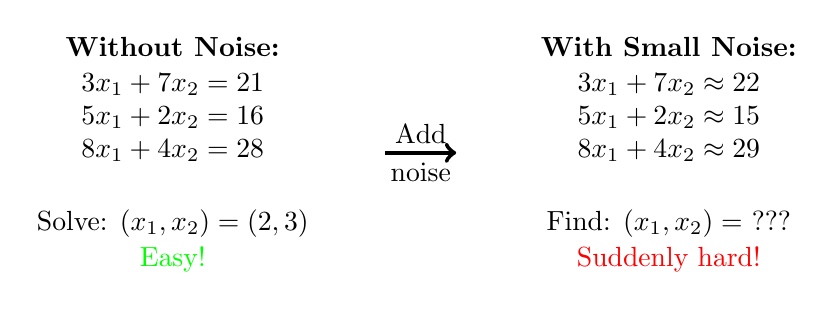
\begin{tikzpicture}[scale=0.9]
    % Clean linear system
    \node at (0,3) {\textbf{Without Noise:}};
    \node[align=left] at (0,2) {
        $3x_1 + 7x_2 = 21$ \\
        $5x_1 + 2x_2 = 16$ \\
        $8x_1 + 4x_2 = 28$
    };
    \node at (0,0.5) {Solve: $(x_1, x_2) = (2, 3)$};
    \node[green] at (0,0) {Easy!};
    
    % Noisy system
    \node at (7,3) {\textbf{With Small Noise:}};
    \node[align=left] at (7,2) {
        $3x_1 + 7x_2 \approx 22$ \\
        $5x_1 + 2x_2 \approx 15$ \\
        $8x_1 + 4x_2 \approx 29$
    };
    \node at (7,0.5) {Find: $(x_1, x_2) = $ ???};
    \node[red] at (7,0) {Suddenly hard!};
    
    % Arrow
    \draw[->, ultra thick] (3,1.5) -- (4,1.5);
    \node[above] at (3.5,1.5) {Add};
    \node[below] at (3.5,1.5) {noise};
\end{tikzpicture}
\caption{LWE in one picture: Noise transforms easy linear algebra into hard problems}
\end{figure}

\begin{definition}[Learning With Errors (Search Version)]
Let $n, q \in \mathbb{N}$, and $\chi$ be an error distribution over $\mathbb{Z}_q$.
\begin{itemize}
    \item \textbf{Secret:} $\mathbf{s} \in \mathbb{Z}_q^n$ (chosen uniformly)
    \item \textbf{Samples:} Many pairs $(\mathbf{a}_i, b_i)$ where:
    \begin{itemize}
        \item $\mathbf{a}_i \in \mathbb{Z}_q^n$ uniform random
        \item $e_i \leftarrow \chi$ (small error)
        \item $b_i = \langle \mathbf{a}_i, \mathbf{s} \rangle + e_i \bmod q$
    \end{itemize}
    \item \textbf{Goal:} Recover $\mathbf{s}$
\end{itemize}
\end{definition}

\begin{example}[Concrete LWE Instance]
Parameters: $n = 4$, $q = 97$, errors in $\{-1, 0, 1\}$

Secret: $\mathbf{s} = (13, 25, 17, 41)$

Sample equations:
\begin{align}
23 \cdot 13 + 67 \cdot 25 + 43 \cdot 17 + 91 \cdot 41 &\equiv 51 \pmod{97} \quad \text{(error = 0)}\\
71 \cdot 13 + 19 \cdot 25 + 84 \cdot 17 + 52 \cdot 41 &\equiv 9 \pmod{97} \quad \text{(error = 1)}\\
45 \cdot 13 + 88 \cdot 25 + 31 \cdot 17 + 76 \cdot 41 &\equiv 74 \pmod{97} \quad \text{(error = -1)}
\end{align}

Without errors: Gaussian elimination in milliseconds.
With errors: Best known algorithm takes exponential time!
\end{example}

\paragraph{The Critical Parameters}

LWE security depends on careful parameter balance:

\begin{definition}[LWE Parameters]
\begin{itemize}
    \item $n$: Dimension (security parameter), typically 500-1000
    \item $q$: Modulus (polynomial in $n$), typically $n^2$ to $n^3$
    \item $\chi$: Error distribution, typically discrete Gaussian
    \item $\alpha = \sigma/q$: Noise rate, typically $1/\sqrt{n}$ to $1/\text{poly}(n)$
\end{itemize}
\end{definition}

\begin{table}[h]
\centering
\begin{tabular}{|l|c|l|}
\hline
\textbf{Parameter} & \textbf{Typical Value} & \textbf{Effect} \\
\hline
Larger $n$ & 512 → 1024 & More security, larger keys \\
Larger $q$ & $2^{13}$ → $2^{15}$ & Easier implementation, weaker security \\
Larger $\sigma$ & 3.2 → 6.4 & More security, higher failure rate \\
More samples $m$ & $n \log q$ & More information for attacker \\
\hline
\end{tabular}
\caption{LWE parameter tradeoffs: Balance security, efficiency, and correctness}
\end{table}

\paragraph{The Error Distribution: Your Noise Model}

For physicists, the error distribution is like choosing your thermal noise model:

\begin{definition}[Discrete Gaussian Distribution]
The discrete Gaussian $D_{\mathbb{Z}, \sigma}$ over integers with parameter $\sigma$:
$$\Pr[X = x] \propto \exp\left(-\frac{x^2}{2\sigma^2}\right)$$
Truncated to $[-B, B]$ where $B = \Theta(\sigma \sqrt{\log n})$ for negligible tail probability.
\end{definition}

\begin{figure}[h]
\centering
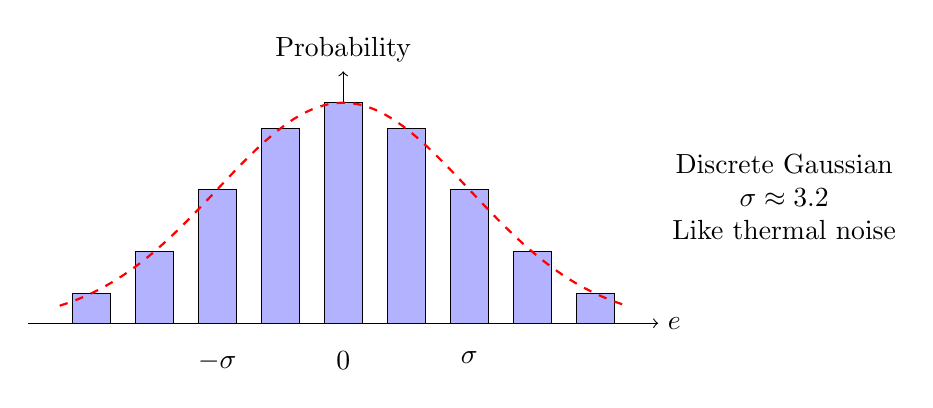
\begin{tikzpicture}[scale=0.8]
    % Axes
    \draw[->] (-5,0) -- (5,0) node[right] {$e$};
    \draw[->] (0,0) -- (0,4) node[above] {Probability};
    
    % Discrete Gaussian bars
    \foreach \x in {-4,-3,-2,-1,0,1,2,3,4} {
        \pgfmathsetmacro\height{3.5*exp(-\x*\x/8)}
        \draw[fill=blue!30] (\x-0.3,0) rectangle (\x+0.3,\height);
    }
    
    % Gaussian envelope
    \draw[thick, red, dashed, domain=-4.5:4.5, samples=100] 
        plot (\x, {3.5*exp(-\x*\x/8)});
    
    % Labels
    \node[below] at (0,-0.3) {0};
    \node[below] at (2,-0.3) {$\sigma$};
    \node[below] at (-2,-0.3) {$-\sigma$};
    
    % Annotation
    \node[align=center] at (7,2) {Discrete Gaussian\\$\sigma \approx 3.2$\\Like thermal noise};
\end{tikzpicture}
\caption{LWE errors: Discrete Gaussian noise hides the secret}
\end{figure}

\paragraph{Search vs Decision: Two Faces of LWE}

\begin{definition}[Decision-LWE]
Distinguish between:
\begin{itemize}
    \item LWE samples: $(\mathbf{a}_i, \langle \mathbf{a}_i, \mathbf{s} \rangle + e_i)$
    \item Uniform random: $(\mathbf{a}_i, u_i)$ where $u_i \in \mathbb{Z}_q$ uniform
\end{itemize}
\end{definition}

\begin{theorem}[Search-Decision Equivalence]
For polynomial $q$ and Gaussian errors, Search-LWE and Decision-LWE are polynomial-time equivalent.
\end{theorem}

This equivalence is crucial: cryptographic security often relies on indistinguishability.

\subsubsection{Why LWE is Hard}

LWE's security rests on one of the most beautiful results in cryptography: average-case LWE is as hard as worst-case lattice problems. This is extraordinary—most cryptographic assumptions are average-case with no worst-case guarantees.

\paragraph{The Worst-Case to Average-Case Connection}

\begin{theorem}[Regev's Reduction (Simplified)]
If you can solve LWE with parameters $(n, q, \chi)$ in polynomial time, then you can solve $\gamma$-SVP on any $n$-dimensional lattice in polynomial time, where:
$$\gamma = \tilde{O}(n\sqrt{q}/\sigma)$$
\end{theorem}

\begin{figure}[h]
\centering
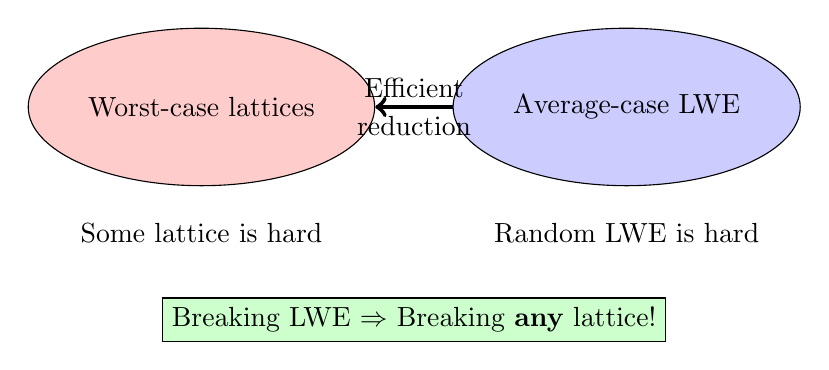
\begin{tikzpicture}[scale=0.9]
    % Worst-case lattices
    \node[draw, ellipse, minimum width=3cm, minimum height=2cm, fill=red!20] 
        (worst) at (0,0) {Worst-case lattices};
    
    % Average-case LWE
    \node[draw, ellipse, minimum width=3cm, minimum height=2cm, fill=blue!20] 
        (avg) at (6,0) {Average-case LWE};
    
    % Reduction arrow
    \draw[->, ultra thick] (avg) -- (worst);
    \node[above] at (3,0) {Efficient};
    \node[below] at (3,0) {reduction};
    
    % Annotations
    \node[below] at (0,-1.5) {Some lattice is hard};
    \node[below] at (6,-1.5) {Random LWE is hard};
    
    % Implication
    \node[draw, rectangle, fill=green!20] at (3,-3) 
        {Breaking LWE $\Rightarrow$ Breaking \textbf{any} lattice!};
\end{tikzpicture}
\caption{LWE's extraordinary guarantee: Average equals worst-case hardness}
\end{figure}

\textbf{Why this matters:}
\begin{itemize}
    \item \textbf{RSA/DH:} No worst-case guarantees (some numbers might be easy to factor)
    \item \textbf{LWE:} If any lattice problem is hard, then random LWE is hard
    \item \textbf{Confidence:} Don't need to avoid "weak instances"
\end{itemize}

\paragraph{The Reduction Intuition: Quantum Fourier Transform Connection}

Here's the brilliant idea behind Regev's reduction, explained for physicists:

\begin{enumerate}
    \item \textbf{Start with any hard lattice} $\mathcal{L}$
    \item \textbf{Use LWE oracle} to learn about $\mathcal{L}$'s dual lattice $\mathcal{L}^*$
    \item \textbf{Apply Quantum Fourier Transform} to connect primal and dual
    \item \textbf{Reconstruct short vectors} in $\mathcal{L}$ from dual information
    \item \textbf{Works for ANY lattice}, not just special ones
\end{enumerate}

\begin{remark}[The Physics of the Quantum Fourier Transform in Regev's Reduction]
For physicists, this is deeply familiar: the quantum Fourier transform (QFT) connects position and momentum representations. In crystallography:
\begin{itemize}
    \item Real space lattice $\leftrightarrow$ Reciprocal (momentum) space lattice
    \item Fourier transform relates the two
    \item Small features in real space $\leftrightarrow$ Large features in reciprocal space
\end{itemize}

Regev's reduction exploits exactly this duality:
\begin{itemize}
    \item LWE samples give noisy information about the dual lattice $\mathcal{L}^*$
    \item QFT converts dual lattice info back to primal lattice
    \item The noise level determines the approximation factor $\gamma$
    \item This is why the original reduction required quantum computation
\end{itemize}

Classical reductions now exist but are more complex and less intuitive.
\end{remark}

\begin{figure}[h]
\centering
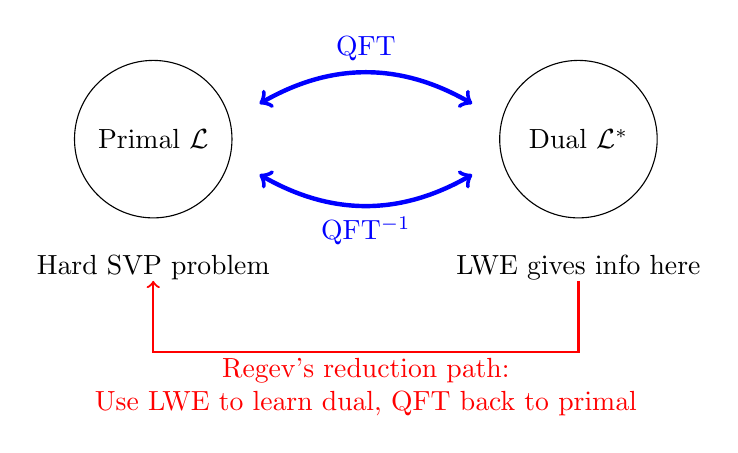
\begin{tikzpicture}[scale=0.9]
    % Primal lattice
    \node[draw, circle, minimum size=2cm] (primal) at (0,0) {Primal $\mathcal{L}$};
    \node[below] at (0,-1.5) {Hard SVP problem};
    
    % Dual lattice
    \node[draw, circle, minimum size=2cm] (dual) at (6,0) {Dual $\mathcal{L}^*$};
    \node[below] at (6,-1.5) {LWE gives info here};
    
    % QFT connection
    \draw[<->, ultra thick, blue] (1.5,0.5) to[bend left=30] node[above] {QFT} (4.5,0.5);
    \draw[<->, ultra thick, blue] (1.5,-0.5) to[bend right=30] node[below] {QFT$^{-1}$} (4.5,-0.5);
    
    % Process flow
    \draw[->, thick, red] (6,-2) -- (6,-3) -- (0,-3) -- (0,-2);
    \node[red, align=center] at (3,-3.5) {Regev's reduction path:\\Use LWE to learn dual, QFT back to primal};
\end{tikzpicture}
\caption{The quantum Fourier transform bridges primal and dual lattices in Regev's reduction}
\end{figure}

\paragraph{Quantum Resistance: Why Shor Doesn't Apply}

LWE resists quantum attack for fundamental reasons:

\begin{theorem}[No Quantum Advantage for LWE]
Best known quantum algorithms for LWE:
\begin{itemize}
    \item Algebraic attacks: No better than classical
    \item Lattice reduction: Polynomial speedup only
    \item Grover search: $\sqrt{q^n}$ time (infeasible for large $n$)
    \item BKZ variants: $2^{0.265n}$ quantum vs $2^{0.292n}$ classical
\end{itemize}
No exponential quantum speedup known after 15+ years.
\end{theorem}

\textbf{Why Shor's algorithm fails:}
\begin{itemize}
    \item \textbf{No periodicity:} LWE samples don't have hidden periods
    \item \textbf{Continuous noise:} Errors destroy any algebraic structure
    \item \textbf{High dimension:} Quantum amplitude spread too thin
    \item \textbf{No group structure:} Can't use hidden subgroup framework
\end{itemize}

\begin{example}[Concrete Quantum Attack on LWE]
Kyber-768 parameters: $n = 256$, $q = 3329$, module rank $k = 3$
\begin{itemize}
    \item Effective lattice dimension: $768$
    \item Classical security: $\approx 2^{180}$
    \item Quantum security: $\approx 2^{164}$
    \item Grover on key: $2^{128}$ (dominates)
    \item Conclusion: 128-bit quantum security achieved
\end{itemize}
\end{example}

\paragraph{Concrete Hardness: From Theory to Practice}

\begin{table}[h]
\centering
\begin{tabular}{|l|c|c|c|c|}
\hline
\textbf{Attack Type} & \textbf{Complexity} & \textbf{Kyber-512} & \textbf{Kyber-768} & \textbf{Kyber-1024} \\
\hline
Primal lattice & $2^{0.292d}$ & $2^{118}$ & $2^{180}$ & $2^{257}$ \\
Dual lattice & $2^{0.292d}$ & $2^{119}$ & $2^{182}$ & $2^{260}$ \\
Algebraic & Unknown & — & — & — \\
Grover key search & $2^{n/2}$ & $2^{128}$ & $2^{128}$ & $2^{128}$ \\
\hline
\textbf{Overall (quantum)} & & \textbf{$2^{107}$} & \textbf{$2^{164}$} & \textbf{$2^{236}$} \\
\hline
\end{tabular}
\caption{LWE security: Multiple attacks, none are efficient}
\end{table}

\subsubsection{LWE-Based Encryption}

Now for the payoff: how to build encryption from LWE. Regev's 2005 scheme remains the template for all modern constructions.

\paragraph{The Geometric Intuition}

Think of LWE encryption as hiding a message in a high-dimensional noise cloud:

\begin{figure}[h]
\centering
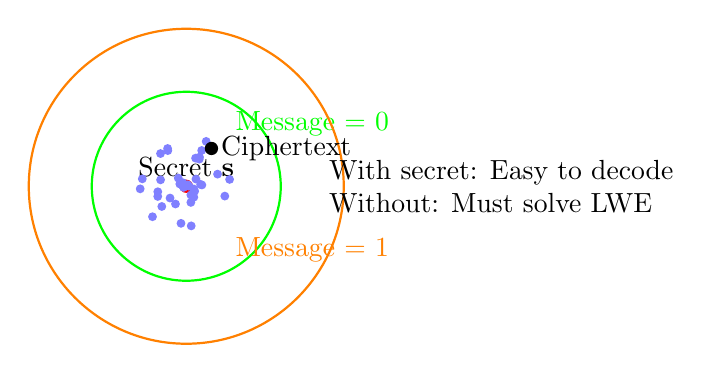
\begin{tikzpicture}[scale=0.8]
    % Secret point
    \fill[red] (3,2) circle (3pt);
    \node[above] at (3,2) {Secret $\mathbf{s}$};
    
    % Noise cloud
    \foreach \i in {1,...,40} {
        \pgfmathsetmacro\angle{random*360}
        \pgfmathsetmacro\radius{random*0.8}
        \pgfmathsetmacro\x{3 + \radius*cos(\angle)}
        \pgfmathsetmacro\y{2 + \radius*sin(\angle)}
        \fill[blue!50] (\x,\y) circle (2pt);
    }
    
    % Message encoding
    \draw[thick, green] (3,2) circle (1.5);
    \node[green] at (5,3) {Message = 0};
    
    \draw[thick, orange] (3,2) circle (2.5);
    \node[orange] at (5,1) {Message = 1};
    
    % Ciphertext point
    \fill[black] (3.4,2.6) circle (3pt);
    \node[right] at (3.4,2.6) {Ciphertext};
    
    % Legend
    \node[align=left] at (8,2) {
        With secret: Easy to decode\\
        Without: Must solve LWE
    };
\end{tikzpicture}
\caption{LWE encryption geometry: Hide messages in noise clouds around secret points}
\end{figure}

\begin{algorithm}
\caption{Regev's LWE Encryption Scheme}
\label{alg:lwe-enc}
\begin{algorithmic}[1]
\State \textbf{Setup:} Parameters $n, q, \chi$, message space $\{0,1\}$

\State \textbf{KeyGen():}
\State \quad $\mathbf{s} \leftarrow \mathbb{Z}_q^n$ \Comment{Secret key}
\State \quad For $i = 1$ to $m = n \log q$:
\State \quad \quad $\mathbf{a}_i \leftarrow \mathbb{Z}_q^n$, $e_i \leftarrow \chi$
\State \quad \quad $b_i = \langle \mathbf{a}_i, \mathbf{s} \rangle + e_i \bmod q$
\State \quad $pk = \{(\mathbf{a}_i, b_i)\}_{i=1}^m$ \Comment{Public key}
\State \quad Return $(pk, sk = \mathbf{s})$

\State \textbf{Encrypt}$(pk, \mu \in \{0,1\})$:
\State \quad $S \subseteq [m]$ random subset
\State \quad $\mathbf{a}' = \sum_{i \in S} \mathbf{a}_i \bmod q$
\State \quad $b' = \sum_{i \in S} b_i + \mu \cdot \lfloor q/2 \rfloor \bmod q$
\State \quad Return $(\mathbf{a}', b')$

\State \textbf{Decrypt}$(sk = \mathbf{s}, (\mathbf{a}', b'))$:
\State \quad $v = b' - \langle \mathbf{a}', \mathbf{s} \rangle \bmod q$
\State \quad If $|v| < q/4$: return 0
\State \quad Else: return 1
\end{algorithmic}
\end{algorithm}

\paragraph{Correctness Analysis}

Why does decryption work? Let's trace through the algebra:

\begin{theorem}[Decryption Correctness]
For ciphertext $(\mathbf{a}', b')$ encrypting $\mu$:
\begin{align}
v &= b' - \langle \mathbf{a}', \mathbf{s} \rangle\\
&= \sum_{i \in S} b_i + \mu \cdot \lfloor q/2 \rfloor - \langle \sum_{i \in S} \mathbf{a}_i, \mathbf{s} \rangle\\
&= \sum_{i \in S} (\langle \mathbf{a}_i, \mathbf{s} \rangle + e_i) + \mu \cdot \lfloor q/2 \rfloor - \sum_{i \in S} \langle \mathbf{a}_i, \mathbf{s} \rangle\\
&= \sum_{i \in S} e_i + \mu \cdot \lfloor q/2 \rfloor\\
&= e_{\text{total}} + \mu \cdot \lfloor q/2 \rfloor
\end{align}
If $|e_{\text{total}}| < q/4$, decryption recovers $\mu$ correctly.
\end{theorem}

\begin{example}[Concrete Encryption]
Parameters: $n = 4$, $q = 97$, message $\mu = 1$

Public key sample: $(\mathbf{a}_1, b_1) = ((23,67,43,91), 51)$

Encryption with subset $S = \{1,3,5\}$:
\begin{itemize}
    \item $\mathbf{a}' = \mathbf{a}_1 + \mathbf{a}_3 + \mathbf{a}_5 = (45, 23, 78, 12)$
    \item $b' = b_1 + b_3 + b_5 + 48 = 51 + 29 + 83 + 48 = 17 \bmod 97$
    \item Ciphertext: $((45,23,78,12), 17)$
\end{itemize}

Decryption:
\begin{itemize}
    \item $v = 17 - \langle(45,23,78,12), (13,25,17,41)\rangle = 17 - 66 = 48 \bmod 97$
    \item Since $48 \approx q/2$, decrypt as $\mu = 1$ \checkmark
\end{itemize}
\end{example}

\paragraph{Security Analysis}

The security proof is remarkably clean:

\begin{theorem}[LWE Encryption Security]
If Decision-LWE is hard, then the encryption scheme is IND-CPA secure.
\end{theorem}

\textbf{Proof sketch:}
\begin{enumerate}
    \item Public key: LWE samples $\{(\mathbf{a}_i, b_i)\}$
    \item By Decision-LWE: Indistinguishable from uniform
    \item Encryption uses random subset sum
    \item Result looks uniform to attacker without $\mathbf{s}$
    \item Message bit hidden by $\lfloor q/2 \rfloor$ offset
\end{enumerate}

\paragraph{From Basic Scheme to Modern Cryptography}

Regev's scheme demonstrates feasibility but isn't practical:
\begin{itemize}
    \item Public keys: $O(n^2 \log q)$ bits
    \item Ciphertexts: $O(n \log q)$ bits  
    \item Only encrypts single bits
\end{itemize}

Modern improvements:
\begin{itemize}
    \item \textbf{Ring-LWE:} Use polynomial structure for compression
    \item \textbf{Module-LWE:} Balance between security and efficiency
    \item \textbf{Better encoding:} Encrypt multiple bits per ciphertext
    \item \textbf{CCA security:} Add authentication via Fujisaki-Okamoto
\end{itemize}

This evolution leads directly to Kyber/ML-KEM, the NIST standard.

\begin{remark}[The Path Forward]
We've shown that:
\begin{itemize}
    \item Lattice problems resist quantum attack
    \item LWE reduces average-case to worst-case hardness
    \item The quantum Fourier transform elegantly connects primal and dual in the reduction
    \item Practical encryption emerges from noisy linear algebra
\end{itemize}
The remaining challenge: efficiency. Ring-LWE and Module-LWE solve this by adding algebraic structure—our next topic.
\end{remark}

\begin{example}[LWE Parameters in Practice]
\begin{center}
\begin{tabular}{|l|c|c|c|c|}
\hline
\textbf{Scheme} & \textbf{$n$} & \textbf{$q$} & \textbf{$\sigma$} & \textbf{Security} \\
\hline
Toy example & 64 & 1,024 & 2.0 & None \\
Learning & 256 & 4,093 & 2.8 & $2^{80}$ \\
Kyber-512 & 256×2 & 3,329 & 1.6 & $2^{128}$ quantum \\
Kyber-768 & 256×3 & 3,329 & 1.6 & $2^{192}$ quantum \\
Kyber-1024 & 256×4 & 3,329 & 1.6 & $2^{256}$ quantum \\
\hline
\end{tabular}
\end{center}
The module dimensions (256×k) show how Ring-LWE improves efficiency.
\end{example}

The beauty of LWE: it transforms the geometric hardness of lattices into the algebraic simplicity of linear equations with noise. This bridge from theory to practice, with the quantum Fourier transform providing the theoretical guarantee, makes lattice-based cryptography not just secure, but implementable at Internet scale.

\subsection{Ring-LWE and Module-LWE}
\label{sec:ring-lwe}

Plain LWE gives us security but at a devastating cost: public keys of megabytes and ciphertexts of kilobytes. For Internet-scale deployment, we need a 100× improvement in efficiency without sacrificing security. The solution comes from an unexpected source: polynomial rings. By adding algebraic structure to our lattices, we achieve dramatic compression while maintaining quantum resistance. This isn't just an optimization—it's the breakthrough that makes post-quantum cryptography practical.

\subsubsection{Efficiency Through Structure}

Let's confront the brutal reality of plain LWE efficiency:

\paragraph{The Key Size Crisis}

\begin{table}[h]
\centering
\begin{tabular}{|l|c|c|c|}
\hline
\textbf{Scheme} & \textbf{Public Key} & \textbf{Ciphertext} & \textbf{Usable?} \\
\hline
RSA-2048 & 256 B & 256 B & Yes \\
ECDH-P256 & 64 B & 64 B & Yes \\
\hline
Plain LWE-512 & 1.6 MB & 2 KB & No \\
Plain LWE-768 & 3.6 MB & 3 KB & No \\
Plain LWE-1024 & 6.4 MB & 4 KB & No \\
\hline
Ring-LWE-512 & 800 B & 768 B & Yes \\
Ring-LWE-768 & 1,184 B & 1,088 B & Yes \\
Ring-LWE-1024 & 1,568 B & 1,568 B & Yes \\
\hline
\end{tabular}
\caption{The efficiency revolution: Ring structure enables 1000× key compression}
\end{table}

\begin{example}[Impact on TLS Handshake]
With plain LWE for 128-bit quantum security:
\begin{itemize}
    \item Each handshake: 1.6 MB public key transmission
    \item Google scale (100B/day): 160 petabytes/day extra
    \item Mobile users: Minutes to establish connection
    \item Certificate chains: 5+ MB with intermediate CAs
    \item Verdict: Completely impractical
\end{itemize}
\end{example}

\paragraph{The Polynomial Ring Solution}

The breakthrough: represent vectors as polynomials and exploit algebraic structure.

\begin{definition}[The Ring $R_q$]
Let $n$ be a power of 2. Define:
$$R = \mathbb{Z}[X]/(X^n + 1) \quad \text{and} \quad R_q = \mathbb{Z}_q[X]/(X^n + 1)$$
Elements are polynomials of degree $< n$ with coefficients in $\mathbb{Z}_q$.
\end{definition}

\textbf{Why polynomials help:}
\begin{itemize}
    \item \textbf{Vector:} $(a_0, a_1, ..., a_{n-1}) \in \mathbb{Z}_q^n$ requires $n$ elements
    \item \textbf{Polynomial:} $a(X) = a_0 + a_1X + ... + a_{n-1}X^{n-1}$ requires $n$ coefficients
    \item \textbf{Magic:} Multiplication by $a(X)$ represents $n \times n$ circulant matrix!
\end{itemize}

\begin{figure}[h]
\centering
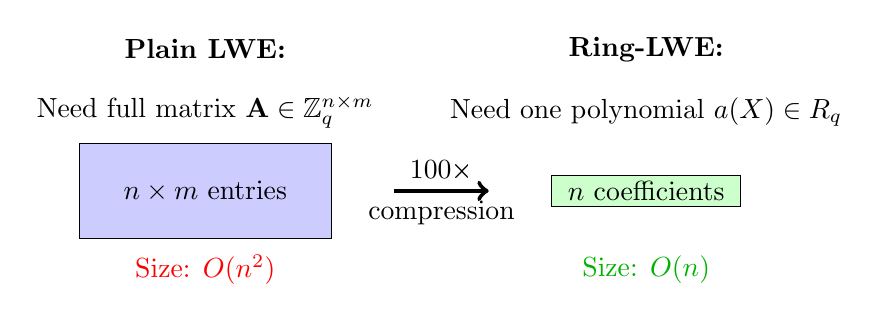
\begin{tikzpicture}[scale=0.8]
    % Vector representation
    \node at (0,3) {\textbf{Plain LWE:}};
    \node at (0,2) {Need full matrix $\mathbf{A} \in \mathbb{Z}_q^{n \times m}$};
    \draw[fill=blue!20] (-2,0) rectangle (2,1.5);
    \node at (0,0.75) {$n \times m$ entries};
    \node[red] at (0,-0.5) {Size: $O(n^2)$};
    
    % Polynomial representation  
    \node at (7,3) {\textbf{Ring-LWE:}};
    \node at (7,2) {Need one polynomial $a(X) \in R_q$};
    \draw[fill=green!20] (5.5,0.5) rectangle (8.5,1);
    \node at (7,0.75) {$n$ coefficients};
    \node[green!70!black] at (7,-0.5) {Size: $O(n)$};
    
    % Arrow showing compression
    \draw[->, ultra thick] (3,0.75) -- (4.5,0.75);
    \node[above] at (3.75,0.75) {100×};
    \node[below] at (3.75,0.75) {compression};
\end{tikzpicture}
\caption{Ring structure enables massive compression without losing information}
\end{figure}

\paragraph{Why $X^n + 1$? The Cyclotomic Choice}

The choice of $X^n + 1$ (where $n = 2^k$) is carefully motivated by both mathematical and practical considerations:

\begin{theorem}[Why Cyclotomic Polynomials Are Optimal]
The polynomial $X^n + 1$ for $n = 2^k$ provides:
\begin{enumerate}
    \item \textbf{Irreducibility:} $X^n + 1$ is the $2n$-th cyclotomic polynomial, irreducible over $\mathbb{Z}$
    \item \textbf{Fast arithmetic:} Enables Number Theoretic Transform (NTT) in $O(n \log n)$
    \item \textbf{Security:} Corresponds to ideal lattices with provable worst-case hardness
    \item \textbf{Implementation:} Powers of 2 optimize memory access and bit operations
\end{enumerate}
\end{theorem}

\begin{remark}[Why Not Other Polynomials?]
You might wonder about alternatives:
\begin{itemize}
    \item $X^n - 1$: Factors as $(X-1)(X^{n-1} + ... + 1)$, not irreducible
    \item $X^p - 1$ (p prime): Gives cyclic convolution, less secure structure
    \item Random irreducible: No fast multiplication algorithm
    \item Other cyclotomics: Less efficient NTT, harder error sampling
\end{itemize}
The choice $X^{2^k} + 1$ uniquely balances all requirements.
\end{remark}

\begin{example}[Multiplication in $R_q$]
Let $n = 4$, $q = 17$. In $R_q = \mathbb{Z}_{17}[X]/(X^4 + 1)$:

$a(X) = 3 + 2X + 5X^2 + X^3$
$b(X) = 1 + 4X + 2X^2 + 3X^3$

Computing $a(X) \cdot b(X)$:
\begin{align}
a \cdot b &= (3 + 2X + 5X^2 + X^3)(1 + 4X + 2X^2 + 3X^3)\\
&= 3 + 14X + 19X^2 + 34X^3 + 21X^4 + 17X^5 + 3X^6\\
&\text{Reduce using } X^4 \equiv -1:\\
&= 3 + 14X + 19X^2 + 34X^3 - 21 - 17X - 3X^2\\
&= -18 + -3X + 16X^2 + 34X^3\\
&\equiv 16 + 14X + 16X^2 + 0X^3 \pmod{17}
\end{align}
\end{example}

\paragraph{The Negacyclic Magic}

Polynomial multiplication in $R_q$ corresponds to matrix-vector multiplication with a special structure:

\begin{equation}
a(X) \cdot b(X) \leftrightarrow 
\begin{pmatrix}
a_0 & -a_{n-1} & -a_{n-2} & \cdots & -a_1 \\
a_1 & a_0 & -a_{n-1} & \cdots & -a_2 \\
a_2 & a_1 & a_0 & \cdots & -a_3 \\
\vdots & \vdots & \vdots & \ddots & \vdots \\
a_{n-1} & a_{n-2} & a_{n-3} & \cdots & a_0
\end{pmatrix}
\begin{pmatrix}
b_0 \\ b_1 \\ b_2 \\ \vdots \\ b_{n-1}
\end{pmatrix}
\end{equation}

One polynomial encodes an entire structured matrix!

\subsubsection{Ring-LWE Definition}

Now we can define the structured version of LWE:

\begin{definition}[Ring Learning With Errors]
Let $R_q = \mathbb{Z}_q[X]/(X^n + 1)$ and $\chi$ be an error distribution over $R$.
\begin{itemize}
    \item \textbf{Secret:} $s \in R_q$ (polynomial with small coefficients)
    \item \textbf{Samples:} Pairs $(a_i, b_i)$ where:
    \begin{itemize}
        \item $a_i \in R_q$ uniformly random
        \item $e_i \leftarrow \chi$ (polynomial with small coefficients)
        \item $b_i = a_i \cdot s + e_i \in R_q$
    \end{itemize}
    \item \textbf{Goal:} Recover $s$
\end{itemize}
\end{definition}

\begin{figure}[h]
\centering
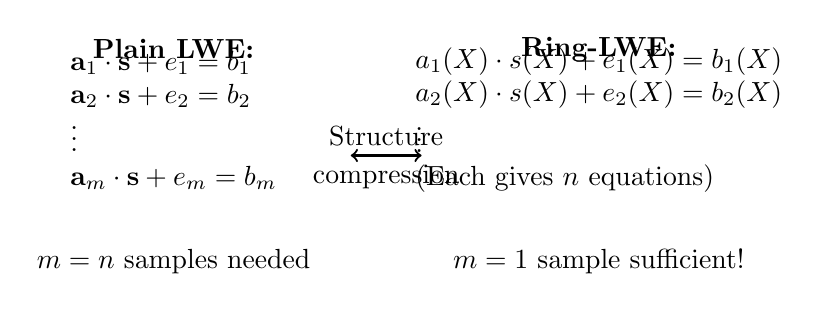
\begin{tikzpicture}[scale=0.9]
    % Plain LWE
    \node at (0,3) {\textbf{Plain LWE:}};
    \node[align=left] at (0,2) {
        $\mathbf{a}_1 \cdot \mathbf{s} + e_1 = b_1$\\
        $\mathbf{a}_2 \cdot \mathbf{s} + e_2 = b_2$\\
        $\vdots$\\
        $\mathbf{a}_m \cdot \mathbf{s} + e_m = b_m$
    };
    \node at (0,0) {$m = n$ samples needed};
    
    % Ring-LWE
    \node at (6,3) {\textbf{Ring-LWE:}};
    \node[align=left] at (6,2) {
        $a_1(X) \cdot s(X) + e_1(X) = b_1(X)$\\
        $a_2(X) \cdot s(X) + e_2(X) = b_2(X)$\\
        $\vdots$\\
        (Each gives $n$ equations)
    };
    \node at (6,0) {$m = 1$ sample sufficient!};
    
    % Comparison
    \draw[<->, thick] (2.5,1.5) -- (3.5,1.5);
    \node[above] at (3,1.5) {Structure};
    \node[below] at (3,1.5) {compression};
\end{tikzpicture}
\caption{Ring-LWE: Each polynomial sample provides $n$ scalar equations}
\end{figure}

\paragraph{Concrete Efficiency Gains}

The improvements are dramatic:

\begin{table}[h]
\centering
\begin{tabular}{|l|c|c|c|}
\hline
\textbf{Operation} & \textbf{Plain LWE} & \textbf{Ring-LWE} & \textbf{Speedup} \\
\hline
Key generation & $O(n^2)$ & $O(n \log n)$ & $100\times$ \\
Encryption & $O(n^2)$ & $O(n \log n)$ & $100\times$ \\
Public key size & $O(n^2 \log q)$ & $O(n \log q)$ & $n\times$ \\
Ciphertext size & $O(n \log q)$ & $O(n \log q)$ & Same \\
\hline
\end{tabular}
\caption{Ring structure improves both time and space complexity}
\end{table}

\begin{example}[Number Theoretic Transform in Practice]
Fast polynomial multiplication using NTT (FFT over finite fields):
\begin{itemize}
    \item Direct multiplication: $O(n^2)$ operations
    \item NTT method: $O(n \log n)$ operations
    \item For $n = 1024$: 100× speedup
    \item Hardware friendly: No floating point needed
    \item Example: Kyber uses $q = 3329 = 13 \cdot 256 + 1$ (NTT-friendly)
\end{itemize}
\end{example}

\subsubsection{Security Considerations}

Adding algebraic structure always raises security concerns. Here's why Ring-LWE remains secure:

\paragraph{The Additional Structure}

Ring-LWE adds structure at multiple levels:

\begin{enumerate}
    \item \textbf{Ideal lattices:} Ring elements correspond to ideals
    \item \textbf{Algebraic relations:} Polynomial multiplication constraints  
    \item \textbf{Symmetries:} Automorphisms of the ring
    \item \textbf{Subfield structure:} For cyclotomic polynomials
\end{enumerate}

\textbf{The security question:} Do these structures enable new attacks?

\paragraph{Why Ring-LWE Remains Secure}

\begin{theorem}[Ring-LWE Hardness (Informal)]
Breaking Ring-LWE for cyclotomic rings reduces to solving worst-case ideal lattice problems. After 15+ years:
\begin{itemize}
    \item No polynomial-time quantum algorithm known
    \item Best attacks only marginally better than plain LWE
    \item Concrete security estimates nearly identical
\end{itemize}
\end{theorem}

\textbf{Failed attack attempts:}
\begin{itemize}
    \item \textbf{2010-2013:} Subfield attacks → Only work for poor parameters
    \item \textbf{2014-2016:} Ideal lattice exploitation → No advantage found
    \item \textbf{2017-2019:} Algebraic number theory attacks → Marginal improvements
    \item \textbf{2020-2023:} Quantum algebraic attacks → No breakthrough
\end{itemize}

\begin{remark}[The Conservative Response]
The cryptographic community's response to potential algebraic attacks: Module-LWE. This hybrid approach balances efficiency and conservative security.
\end{remark}

\paragraph{Module-LWE: The Best of Both Worlds}

\begin{definition}[Module Learning With Errors]
Work over $R_q^k$ for small $k$ (typically 2-4):
\begin{itemize}
    \item Elements: Vectors of polynomials $(f_1(X), ..., f_k(X))$
    \item Operations: Matrix-vector multiplication over $R_q$
    \item Structure: Between plain LWE ($k = n$) and Ring-LWE ($k = 1$)
\end{itemize}
\end{definition}

\begin{figure}[h]
\centering
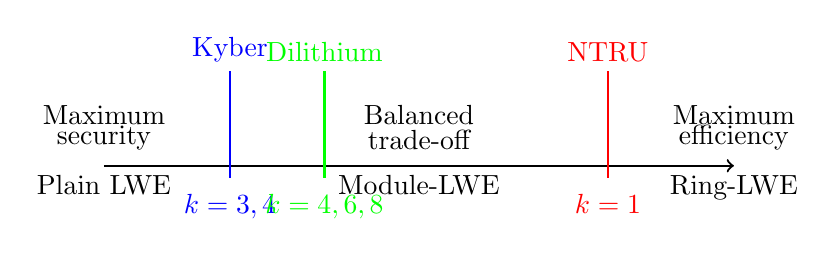
\begin{tikzpicture}[scale=0.8]
    % Spectrum
    \draw[thick, ->] (0,0) -- (10,0);
    \node[below] at (0,0) {Plain LWE};
    \node[below] at (10,0) {Ring-LWE};
    \node[below] at (5,0) {Module-LWE};
    
    % Properties
    \node[above] at (0,0.5) {Maximum};
    \node[above] at (0,0.1) {security};
    
    \node[above] at (10,0.5) {Maximum};
    \node[above] at (10,0.1) {efficiency};
    
    \node[above] at (5,0.5) {Balanced};
    \node[above] at (5,0.1) {trade-off};
    
    % Actual schemes
    \draw[thick, blue] (2,1.5) -- (2,-0.2);
    \node[above, blue] at (2,1.5) {Kyber};
    \node[below, blue] at (2,-0.3) {$k=3,4$};
    
    \draw[thick, green] (3.5,1.5) -- (3.5,-0.2);
    \node[above, green] at (3.5,1.5) {Dilithium};
    \node[below, green] at (3.5,-0.3) {$k=4,6,8$};
    
    \draw[thick, red] (8,1.5) -- (8,-0.2);
    \node[above, red] at (8,1.5) {NTRU};
    \node[below, red] at (8,-0.3) {$k=1$};
\end{tikzpicture}
\caption{Module-LWE provides flexible security-efficiency trade-offs}
\end{figure}

\begin{example}[Concrete Module-LWE Operations]
Let's see Module-LWE in action with Kyber-768 parameters:
\begin{itemize}
    \item Ring: $R_q = \mathbb{Z}_{3329}[X]/(X^{256} + 1)$
    \item Module dimension: $k = 3$
    \item Secret: $\mathbf{s} = (s_1(X), s_2(X), s_3(X)) \in R_q^3$
    \item Public key matrix: $\mathbf{A} \in R_q^{3 \times 3}$
\end{itemize}

Key generation:
$$\mathbf{t} = \mathbf{A} \mathbf{s} + \mathbf{e} = \begin{pmatrix}
a_{11} & a_{12} & a_{13} \\
a_{21} & a_{22} & a_{23} \\
a_{31} & a_{32} & a_{33}
\end{pmatrix} \begin{pmatrix}
s_1 \\ s_2 \\ s_3
\end{pmatrix} + \begin{pmatrix}
e_1 \\ e_2 \\ e_3
\end{pmatrix}$$

Each $a_{ij}, s_i, e_i$ is a polynomial in $R_q$. The matrix multiplication involves:
\begin{itemize}
    \item 9 polynomial multiplications (NTT-accelerated)
    \item 6 polynomial additions
    \item Total: $9 \times 256 \times \log(256) \approx 18,000$ operations
    \item Compare plain LWE: $768^2 \approx 590,000$ operations
\end{itemize}
\end{example}

\textbf{Why NIST chose Module-LWE:}
\begin{itemize}
    \item \textbf{Conservative:} Less algebraic structure than pure Ring-LWE
    \item \textbf{Efficient:} Much better than plain LWE
    \item \textbf{Flexible:} Adjust $k$ for different security levels
    \item \textbf{Proven:} Worst-case hardness still holds
\end{itemize}

\paragraph{Parameter Selection Rationale}

Choosing parameters requires balancing multiple constraints:

\begin{table}[h]
\centering
\begin{tabular}{|l|l|l|}
\hline
\textbf{Parameter} & \textbf{Constraint} & \textbf{Typical Choice} \\
\hline
$n$ (ring dimension) & Power of 2 for NTT & 256, 512, 1024 \\
$q$ (modulus) & NTT-friendly, small & 3329, 7681, 12289 \\
$k$ (module rank) & Security/efficiency balance & 2, 3, 4 \\
$\eta$ (error bound) & Correctness vs security & 2, 3 \\
\hline
\end{tabular}
\caption{Parameter choices balance security, efficiency, and implementation}
\end{table}

\begin{example}[Kyber's Parameter Choices]
Why Kyber chose $n = 256$, $q = 3329$:
\begin{itemize}
    \item $n = 256 = 2^8$: Optimal for AVX2 (8×32-bit registers)
    \item $q = 3329 = 13 \cdot 256 + 1$: 
    \begin{itemize}
        \item Smallest prime $> 12 \cdot \eta \cdot \sqrt{n}$ (correctness)
        \item $= 1 \bmod 2n$ (NTT exists)
        \item Fits in 12 bits (efficient storage)
    \end{itemize}
    \item Module dimensions: $k \in \{2, 3, 4\}$ for NIST levels I, III, V
    \item Total dimension: $256k$ matches security requirements
\end{itemize}
\end{example}

\paragraph{Performance in Practice}

Real-world benchmarks show the dramatic improvement:

\begin{table}[h]
\centering
\begin{tabular}{|l|c|c|c|}
\hline
\textbf{Operation} & \textbf{RSA-2048} & \textbf{Plain LWE} & \textbf{Kyber-768} \\
\hline
KeyGen & 100 ms & 50 ms & 0.1 ms \\
Encapsulation & 0.05 ms & 20 ms & 0.12 ms \\
Decapsulation & 2 ms & 15 ms & 0.11 ms \\
Public key & 256 B & 1.6 MB & 1,184 B \\
Ciphertext & 256 B & 2 KB & 1,088 B \\
\hline
\end{tabular}
\caption{Module-LWE (Kyber) is faster than RSA with reasonable key sizes}
\end{table}

\paragraph{The Bottom Line on Structure}

After 15+ years of intensive cryptanalysis:
\begin{itemize}
    \item Ring structure provides 100-1000× efficiency gain
    \item No significant security loss discovered
    \item Module structure offers conservative middle ground
    \item Enables practical post-quantum deployment
\end{itemize}

\begin{remark}[For the Physics-Minded]
Think of this as symmetry in physics: adding symmetry (ring structure) constrains the system but often makes problems easier to solve. In cryptography, we've found a sweet spot where the efficiency gains are massive but the security loss is negligible. It's like finding a crystal structure that's both stable and useful.
\end{remark}

\begin{example}[Migration Impact]
With Ring/Module-LWE, post-quantum transition becomes feasible:
\begin{itemize}
    \item TLS handshake overhead: 2× instead of 1000×
    \item Certificate sizes: 5 KB instead of 5 MB
    \item IoT devices: Possible with constrained memory
    \item Performance: Often faster than current algorithms
\end{itemize}
Without this structure, PQC would remain theoretical.
\end{example}

The journey from abstract lattices to practical cryptography required two breakthroughs: LWE showed how to use lattice hardness, and Ring-LWE made it efficient. Module-LWE provides the conservative balance that convinced NIST. This combination gives us quantum-resistant cryptography that works at Internet scale. Now we can examine how NIST transformed these ideas into concrete standards.

\subsection{NIST Lattice-Based Standards}
\label{sec:nist-standards}

After five years of intense global competition, NIST selected three lattice-based algorithms as standards for post-quantum cryptography. This wasn't just an academic exercise—these algorithms will protect trillions of dollars in commerce, secure government communications for decades, and safeguard personal privacy in the quantum era. Understanding why NIST chose these specific algorithms, and how they differ, is crucial for anyone deploying post-quantum security.

\subsubsection{NIST Competition Process}

The NIST Post-Quantum Cryptography Standardization Process represents the largest coordinated cryptographic evaluation in history.

\paragraph{Timeline: From Crisis to Standards}

\begin{figure}[h]
\centering
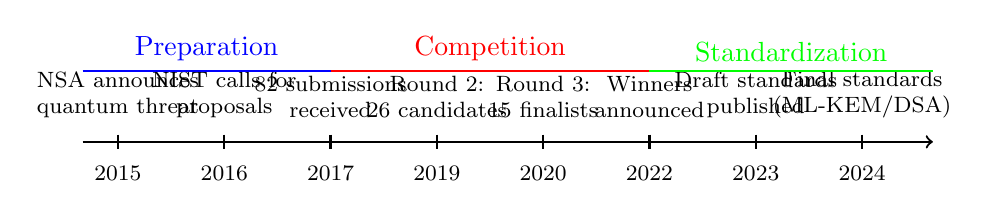
\begin{tikzpicture}[scale=0.9]
    % Timeline
    \draw[thick, ->] (0,0) -- (12,0);
    
    % Major events
    \foreach \x/\year/\event in {
        0.5/2015/{NSA announces}\\ {quantum threat},
        2/2016/{NIST calls for}\\ {proposals},
        3.5/2017/{82 submissions}\\ {received},
        5/2019/{Round 2:}\\ {26 candidates},
        6.5/2020/{Round 3:}\\ {15 finalists},
        8/2022/{Winners}\\ {announced},
        9.5/2023/{Draft standards}\\ {published},
        11/2024/{Final standards}\\ {(ML-KEM/DSA)}
    } {
        \draw[thick] (\x,0.1) -- (\x,-0.1);
        \node[below, align=center, font=\footnotesize] at (\x,-0.2) {\year};
        \node[above, align=center, font=\footnotesize] at (\x,0.2) {\event};
    }
    
    % Phases
    \draw[thick, blue] (0,1) -- (3.5,1);
    \node[above, blue] at (1.75,1) {Preparation};
    
    \draw[thick, red] (3.5,1) -- (8,1);
    \node[above, red] at (5.75,1) {Competition};
    
    \draw[thick, green] (8,1) -- (12,1);
    \node[above, green] at (10,1) {Standardization};
\end{tikzpicture}
\caption{NIST PQC timeline: 9 years from recognition to deployment}
\end{figure}

\paragraph{The Competition Details}

The process was unprecedented in scope and transparency:

\begin{itemize}
    \item \textbf{82 initial submissions:} From academia, industry, and governments worldwide
    \item \textbf{69 complete packages:} Meeting all requirements
    \item \textbf{Public evaluation:} All submissions, analyses, and attacks published
    \item \textbf{3 PQC conferences:} Community feedback and cryptanalysis
    \item \textbf{100+ researchers:} Active participants in evaluation
    \item \textbf{1000+ papers:} Published analyses and improvements
\end{itemize}

\paragraph{Evaluation Criteria: Beyond Just Security}

NIST evaluated candidates on multiple dimensions:

\begin{table}[h]
\centering
\begin{tabular}{|l|l|c|}
\hline
\textbf{Criterion} & \textbf{Description} & \textbf{Weight} \\
\hline
Security & Resistance to classical/quantum attack & 40\% \\
Performance & Speed on various platforms & 20\% \\
Key/signature sizes & Bandwidth and storage impact & 20\% \\
Implementation & Side-channel resistance, simplicity & 10\% \\
Flexibility & Parameter choices, crypto-agility & 5\% \\
Maturity & Years of analysis, confidence level & 5\% \\
\hline
\end{tabular}
\caption{NIST's holistic evaluation went far beyond theoretical security}
\end{table}

\begin{example}[Real Evaluation Trade-offs]
Rainbow (multivariate signatures):
\begin{itemize}
    \item \checkmark Tiny signatures (66 bytes!)
    \item \checkmark Fast verification
    \item \xmark Huge public keys (158 KB)
    \item \xmark Broken in 2022 by new attack
\end{itemize}
Lesson: Multiple criteria prevent single-point optimization.
\end{example}

\paragraph{Algorithm Naming Conventions}

Understanding the naming helps navigate the standards:

\begin{itemize}
    \item \textbf{CRYSTALS:} Cryptographic Suite for Algebraic Lattices
    \begin{itemize}
        \item Kyber → ML-KEM (Module Lattice-Based KEM)
        \item Dilithium → ML-DSA (Module Lattice-Based Digital Signature Algorithm)
    \end{itemize}
    \item \textbf{Falcon:} Fast Fourier Lattice-based Compact Signatures over NTRU
    \item \textbf{SPHINCS+:} Not lattice-based (hash-based signatures)
\end{itemize}

\paragraph{Why Multiple Winners?}

NIST's philosophy: diversification protects against catastrophic failure.

\begin{figure}[h]
\centering
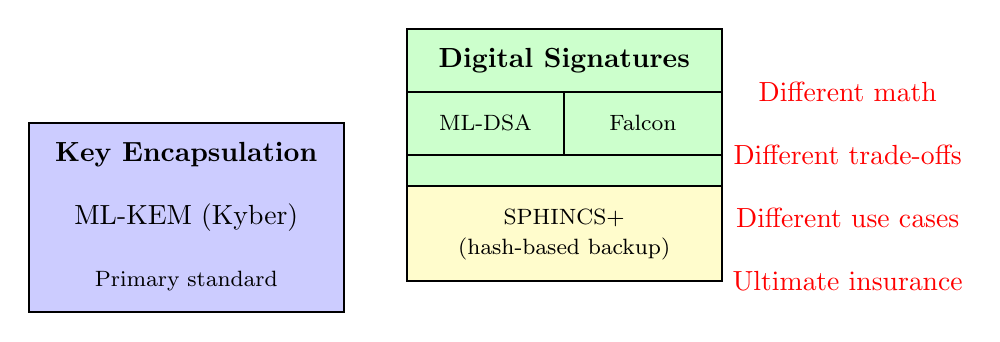
\begin{tikzpicture}[scale=0.8]
    % KEM box
    \draw[thick, fill=blue!20] (0,0) rectangle (5,3);
    \node[font=\bfseries] at (2.5,2.5) {Key Encapsulation};
    \node at (2.5,1.5) {ML-KEM (Kyber)};
    \node[font=\footnotesize] at (2.5,0.5) {Primary standard};
    
    % Signature boxes
    \draw[thick, fill=green!20] (6,1.5) rectangle (11,4.5);
    \node[font=\bfseries] at (8.5,4) {Digital Signatures};
    
    \draw[thick] (6,2.5) rectangle (8.5,3.5);
    \node[font=\footnotesize] at (7.25,3) {ML-DSA};
    
    \draw[thick] (8.5,2.5) rectangle (11,3.5);
    \node[font=\footnotesize] at (9.75,3) {Falcon};
    
    \draw[thick, fill=yellow!20] (6,0.5) rectangle (11,2);
    \node[font=\footnotesize] at (8.5,1.5) {SPHINCS+};
    \node[font=\footnotesize] at (8.5,1) {(hash-based backup)};
    
    % Annotations
    \node[red] at (13,3.5) {Different math};
    \node[red] at (13,2.5) {Different trade-offs};
    \node[red] at (13,1.5) {Different use cases};
    \node[red] at (13,0.5) {Ultimate insurance};
\end{tikzpicture}
\caption{NIST's portfolio approach: Multiple algorithms for resilience}
\end{figure}

\paragraph{Why SPHINCS+ Wasn't Covered}

SPHINCS+ is NIST's insurance policy—a hash-based signature scheme:
\begin{itemize}
    \item \textbf{Security:} Based only on hash function security (SHA-256)
    \item \textbf{Quantum-safe:} Even if all lattice problems fall
    \item \textbf{Trade-off:} Large signatures (8-50 KB)
    \item \textbf{Use case:} Emergency backup, firmware signing
    \item \textbf{Not lattice-based:} Outside our current scope
\end{itemize}

\paragraph{Patent Considerations}

NIST required all submissions to be available royalty-free:
\begin{itemize}
    \item All selected algorithms: Patent-free worldwide
    \item Some candidates withdrawn due to IP issues
    \item NTRU patents expired before selection
    \item Clear legal status critical for global adoption
\end{itemize}

\subsubsection{CRYSTALS-Kyber (ML-KEM)}

Kyber, now standardized as ML-KEM (Module Lattice-Based Key Encapsulation Mechanism), is NIST's primary choice for key establishment.

\paragraph{Why Kyber Won}

Kyber achieved the best overall balance:
\begin{itemize}
    \item \textbf{Security:} Conservative Module-LWE foundation
    \item \textbf{Efficiency:} Competitive with elliptic curves
    \item \textbf{Simplicity:} Clean implementation without footguns
    \item \textbf{Flexibility:} Three parameter sets for different needs
\end{itemize}

\paragraph{Technical Foundation}

\begin{algorithm}
\caption{ML-KEM (Kyber) Overview}
\label{alg:kyber}
\begin{algorithmic}[1]
\State \textbf{Parameters:} $(n, k, q, \eta_1, \eta_2, d_u, d_v)$
\State Ring: $R_q = \mathbb{Z}_q[X]/(X^n + 1)$ where $n = 256$, $q = 3329$

\State \textbf{KeyGen():}
\State \quad $\mathbf{A} \leftarrow R_q^{k \times k}$ (seed expansion)
\State \quad $\mathbf{s}, \mathbf{e} \leftarrow \beta_\eta^{k}$ (small secrets)
\State \quad $\mathbf{t} = \mathbf{A}\mathbf{s} + \mathbf{e}$
\State \quad $pk = (\mathbf{t}, \text{seed}(\mathbf{A}))$, $sk = \mathbf{s}$

\State \textbf{Encapsulate}$(pk)$:
\State \quad $\mathbf{r}, \mathbf{e}_1, e_2 \leftarrow \beta_\eta$ (small noise)
\State \quad $\mathbf{u} = \mathbf{A}^T\mathbf{r} + \mathbf{e}_1$
\State \quad $v = \mathbf{t}^T\mathbf{r} + e_2 + \lfloor q/2 \rceil \cdot m$
\State \quad $c = (\text{Compress}(\mathbf{u}), \text{Compress}(v))$
\State \quad $K = \text{KDF}(m, H(c))$

\State \textbf{Decapsulate}$(sk, c)$:
\State \quad Decompress and compute $v - \mathbf{s}^T\mathbf{u}$
\State \quad Recover $m$ and recompute $K$
\end{algorithmic}
\end{algorithm}

\textbf{Key innovations:}
\begin{itemize}
    \item \textbf{Compression:} Reduce ciphertext size by dropping LSBs
    \item \textbf{Error reconciliation:} Ensure both parties get same key
    \item \textbf{CCA security:} Fujisaki-Okamoto transform built-in
    \item \textbf{Deterministic noise:} Reduces randomness requirements
\end{itemize}

\paragraph{Parameter Sets and Security}

\begin{table}[h]
\centering
\begin{tabular}{|l|c|c|c|c|c|}
\hline
\textbf{Parameter Set} & \textbf{$k$} & \textbf{Security} & \textbf{PK (bytes)} & \textbf{CT (bytes)} & \textbf{SS (bytes)} \\
\hline
ML-KEM-512 & 2 & 128-bit quantum & 800 & 768 & 32 \\
ML-KEM-768 & 3 & 192-bit quantum & 1,184 & 1,088 & 32 \\
ML-KEM-1024 & 4 & 256-bit quantum & 1,568 & 1,568 & 32 \\
\hline
\multicolumn{6}{c}{For comparison:} \\
\hline
X25519 & — & 128-bit classical & 32 & 32 & 32 \\
RSA-2048 & — & 112-bit classical & 256 & 256 & 256 \\
\hline
\end{tabular}
\caption{ML-KEM parameters: 30-40× larger than ECC but still practical}
\end{table}

\paragraph{Performance Characteristics}

Real-world benchmarks on Intel Core i7-8700K @ 3.7GHz, AVX2 enabled, GCC 11.2:

\begin{table}[h]
\centering
\begin{tabular}{|l|c|c|c|}
\hline
\textbf{Operation} & \textbf{ML-KEM-768} & \textbf{X25519} & \textbf{Ratio} \\
\hline
KeyGen & 35 µs & 45 µs & 0.8× \\
Encapsulate & 44 µs & 45 µs & 1.0× \\
Decapsulate & 40 µs & 45 µs & 0.9× \\
\hline
\end{tabular}
\caption{ML-KEM matches or beats elliptic curve performance!}
\end{table}

\begin{remark}[The Surprise]
Lattice operations (integer arithmetic + NTT) are so efficient that ML-KEM often outperforms elliptic curves despite working in dimension 768 vs. 256-bit scalars. This wasn't expected when the competition began.
\end{remark}

\paragraph{Hybrid Mode Deployment}

For transitional security, NIST recommends hybrid modes:

\begin{definition}[Hybrid Key Exchange]
Combine classical and post-quantum algorithms:
$$\text{SharedSecret} = \text{KDF}(\text{ECDH\_Secret} || \text{ML-KEM\_Secret})$$
\end{definition}

\textbf{Why hybrid modes matter:}
\begin{itemize}
    \item \textbf{Belt and suspenders:} Security if either algorithm holds
    \item \textbf{Transition period:} Maintain compatibility
    \item \textbf{Standards:} X25519+ML-KEM-768 for TLS 1.3
    \item \textbf{Overhead:} Only ~1.3 KB extra vs pure ML-KEM
\end{itemize}

\begin{example}[TLS 1.3 Hybrid Handshake]
Client and server negotiate:
\begin{itemize}
    \item Classical: X25519 (32 byte public key)
    \item Post-quantum: ML-KEM-768 (1,184 byte public key)
    \item Combined: 1,216 bytes total
    \item Security: Best of both worlds
    \item Performance: Negligible impact (< 5\% slower)
\end{itemize}
\end{example}

\subsubsection{CRYSTALS-Dilithium (ML-DSA)}

Dilithium, standardized as ML-DSA (Module Lattice-Based Digital Signature Algorithm), is NIST's primary signature scheme.

\paragraph{The Signature Challenge}

Digital signatures from lattices are harder than encryption:
\begin{itemize}
    \item Signatures reveal information about the secret key
    \item Must ensure no leakage across many signatures
    \item Size-security trade-offs more challenging
    \item Need rejection sampling for security
\end{itemize}

\paragraph{Dilithium's Approach: Fiat-Shamir with Aborts}

\begin{algorithm}
\caption{ML-DSA (Dilithium) Signing - Simplified}
\label{alg:dilithium}
\begin{algorithmic}[1]
\State \textbf{Input:} Message $M$, secret key $(\mathbf{s}_1, \mathbf{s}_2)$
\State \textbf{Output:} Signature $(\mathbf{z}, \mathbf{h}, c)$

\Repeat
    \State $\mathbf{y} \leftarrow S_\gamma$ \Comment{Large masking vector}
    \State $\mathbf{w} = \mathbf{A}\mathbf{y}$ \Comment{Commitment}
    \State $c = H(\mathbf{w}_{\text{high}} || M)$ \Comment{Challenge}
    \State $\mathbf{z} = \mathbf{y} + c\mathbf{s}_1$ \Comment{Response}
    \State \textbf{if} $||\mathbf{z}||_\infty \geq \gamma - \beta$ \textbf{then}
    \State \quad \textbf{restart} \Comment{Abort to prevent leakage!}
    \State \textbf{endif}
\Until{signature accepted}
\State Compute hint $\mathbf{h}$ for verification
\State \Return $(\mathbf{z}, \mathbf{h}, c)$
\end{algorithmic}
\end{algorithm}

\textbf{Key insight:} Rejection sampling ensures the signature distribution is independent of the secret key!

\begin{figure}[h]
\centering
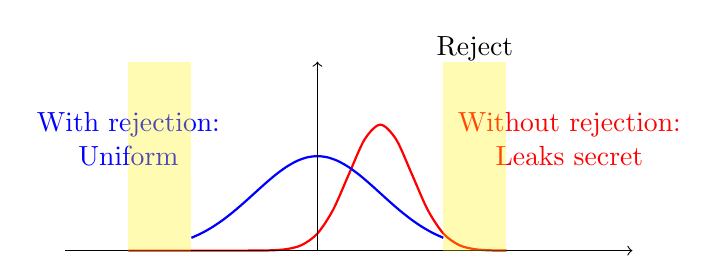
\begin{tikzpicture}[scale=0.8]
    % Distribution without rejection
    \draw[thick, red] plot[smooth, domain=-3:3] (\x, {2*exp(-(\x-1)*(\x-1)/0.5)});
    \node[red] at (4,2) {Without rejection:};
    \node[red] at (4,1.5) {Leaks secret};
    
    % Distribution with rejection
    \draw[thick, blue] plot[smooth, domain=-2:2] (\x, {1.5*exp(-\x*\x/2)});
    \node[blue] at (-3,2) {With rejection:};
    \node[blue] at (-3,1.5) {Uniform};
    
    % Axes
    \draw[->] (-4,0) -- (5,0);
    \draw[->] (0,0) -- (0,3);
    
    % Rejection region
    \fill[yellow, opacity=0.3] (2,0) rectangle (3,3);
    \fill[yellow, opacity=0.3] (-3,0) rectangle (-2,3);
    \node at (2.5,3.2) {Reject};
\end{tikzpicture}
\caption{Rejection sampling: Sacrifice efficiency for perfect security}
\end{figure}

\paragraph{Parameter Sets and Trade-offs}

\begin{table}[h]
\centering
\begin{tabular}{|l|c|c|c|c|c|}
\hline
\textbf{Level} & \textbf{Security} & \textbf{PK (bytes)} & \textbf{Sig (bytes)} & \textbf{Sign/s} & \textbf{Verify/s} \\
\hline
ML-DSA-44 & 128-bit & 1,312 & 2,420 & 3,700 & 9,100 \\
ML-DSA-65 & 192-bit & 1,952 & 3,309 & 2,500 & 6,200 \\
ML-DSA-87 & 256-bit & 2,592 & 4,627 & 1,900 & 4,600 \\
\hline
\multicolumn{6}{c}{For comparison:} \\
\hline
Ed25519 & 128-bit classical & 32 & 64 & 24,000 & 8,000 \\
RSA-2048 & 112-bit classical & 256 & 256 & 500 & 17,000 \\
\hline
\end{tabular}
\caption{ML-DSA: Larger signatures but competitive performance. Benchmarks on Intel Core i7-8700K.}
\end{table}

\textbf{Why these trade-offs are acceptable:}
\begin{itemize}
    \item Signatures are usually transmitted once, verified many times
    \item 3 KB is tiny compared to typical signed data
    \item Verification speed matches current algorithms
    \item Signing speed sufficient for most applications
\end{itemize}

\begin{example}[TLS Certificate Chain Impact]
Current TLS with RSA-2048:
\begin{itemize}
    \item 3 certificates × 256 bytes = 768 bytes signatures
    \item Total certificate chain: ~4 KB
\end{itemize}

With ML-DSA-44:
\begin{itemize}
    \item 3 certificates × 2,420 bytes = 7,260 bytes signatures
    \item Total certificate chain: ~11 KB
    \item Impact: 7 KB extra per handshake (acceptable)
\end{itemize}
\end{example}

\subsubsection{Falcon}

Falcon represents a different approach: using NTRU lattices and advanced sampling techniques to achieve the smallest signatures.

\paragraph{The NTRU Heritage}

Falcon builds on NTRU, one of the oldest lattice schemes (1996):

\begin{definition}[NTRU Lattice Structure]
Work in ring $R = \mathbb{Z}[X]/(X^n + 1)$ with:
\begin{itemize}
    \item Public key: $h = f^{-1} \cdot g$ where $f, g$ small
    \item Secret key: The "good" basis $(f, g)$
    \item Signing: Use secret basis to solve CVP efficiently
    \item Security: Finding good basis from $h$ is hard
\end{itemize}
\end{definition}

\paragraph{Gaussian Sampling: The Technical Challenge}

Falcon's key operation is sampling from a discrete Gaussian over a lattice:

\begin{figure}[h]
\centering
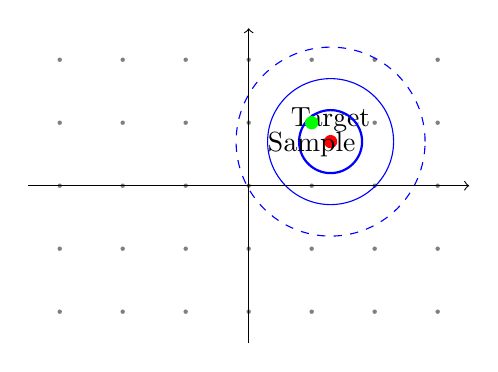
\begin{tikzpicture}[scale=0.8]
    % Lattice points
    \foreach \i in {-3,-2,-1,0,1,2,3} {
        \foreach \j in {-2,-1,0,1,2} {
            \fill[gray] (\i,\j) circle (1pt);
        }
    }
    
    % Target point
    \fill[red] (1.3,0.7) circle (3pt);
    \node[above] at (1.3,0.7) {Target};
    
    % Gaussian contours
    \draw[blue, thick] (1.3,0.7) circle (0.5);
    \draw[blue] (1.3,0.7) circle (1);
    \draw[blue, dashed] (1.3,0.7) circle (1.5);
    
    % Sampled point
    \fill[green] (1,1) circle (3pt);
    \node[below] at (1,1) {Sample};
    
    % Axes for illustration
    \draw[->] (-3.5,0) -- (3.5,0);
    \draw[->] (0,-2.5) -- (0,2.5);
\end{tikzpicture}
\caption{Falcon samples lattice points near targets with Gaussian probability}
\end{figure}

\textbf{WARNING: Falcon's Implementation Complexity}

Falcon is notoriously difficult to implement securely:
\begin{itemize}
    \item \textbf{Floating-point arithmetic:} Requires IEEE 754 double precision (53+ bits)
    \item \textbf{Platform dependence:} Different FP behavior across CPUs
    \item \textbf{Side-channel vulnerability:} FP operations leak timing information
    \item \textbf{No constant-time guarantee:} Branch-free implementation extremely difficult
    \item \textbf{Memory access patterns:} Can leak secret key information
\end{itemize}

\begin{lstlisting}[language=C, caption=Falcon's Precision Requirements - DO NOT USE IN PRODUCTION WITHOUT EXPERTISE]
// Gaussian sampling requires high precision
typedef struct {
    double real;  // MUST be IEEE 754 double
    double imag;  // Rounding errors can break security
} complex;

// Fast Fourier sampling over complex numbers
void FFT(complex *f, unsigned logn) {
    // WARNING: Not constant-time!
    // Side-channel attacks possible
    // Different results on different platforms
    // Requires expert implementation
}

// Compare to Dilithium:
// Only needs uint32_t arithmetic
// Naturally constant-time
// Platform independent
\end{lstlisting}

\paragraph{Falcon's Trade-offs}

\begin{table}[h]
\centering
\begin{tabular}{|l|c|c|}
\hline
\textbf{Aspect} & \textbf{Advantage} & \textbf{Disadvantage} \\
\hline
Signature size & Smallest (666-1,280 bytes) & Still 10× Ed25519 \\
Verification & Very fast & — \\
Public key & Compact (897-1,793 bytes) & — \\
Signing & — & Complex implementation \\
Side-channels & — & Extremely hard to protect \\
Platforms & — & Needs FP unit \\
Implementation & — & Few correct implementations \\
\hline
\end{tabular}
\caption{Falcon: Optimal sizes at the cost of severe implementation complexity}
\end{table}

\begin{example}[Where Falcon Shines]
Blockchain transaction:
\begin{itemize}
    \item Thousands of signatures stored forever
    \item Size matters more than signing speed
    \item Falcon-512: 666 bytes vs. Dilithium: 2,420 bytes
    \item Saves 1.7 KB per transaction
    \item 1 million transactions: 1.7 GB saved
    \item BUT: Requires expert implementation team
\end{itemize}
\end{example}

\paragraph{NIST's Warning on Falcon}

NIST's official stance on Falcon is cautious:

\begin{quote}
"Falcon is suitable for applications where signature size is critical and implementation expertise is available. Organizations should carefully evaluate whether they have the necessary expertise to implement Falcon securely. For most applications, ML-DSA is the recommended choice."
\end{quote}

\textbf{Real-world Falcon challenges:}
\begin{itemize}
    \item \textbf{ARM Cortex-M:} No FPU, software emulation too slow
    \item \textbf{Intel vs AMD:} Different FP rounding can break interoperability
    \item \textbf{Timing attacks:} Multiple academic papers show vulnerabilities
    \item \textbf{Reference implementation:} Not production-ready
    \item \textbf{Hardware support:} Requires custom FP units for safety
\end{itemize}

\paragraph{Deployment Recommendations}

\begin{table}[h]
\centering
\begin{tabular}{|l|l|l|}
\hline
\textbf{Use Case} & \textbf{Recommendation} & \textbf{Reason} \\
\hline
TLS/HTTPS & ML-DSA & Easier implementation \\
Code signing & ML-DSA & Broad platform support \\
Email (S/MIME) & ML-DSA & Standard compliance \\
Blockchain & Falcon (maybe) & Size critical, but risky \\
IoT devices & ML-DSA & No FP needed \\
HSMs & Falcon (with care) & Controlled environment \\
General purpose & ML-DSA & Always safer choice \\
\hline
\end{tabular}
\caption{Choose ML-DSA by default, Falcon only with expert teams}
\end{table}

\begin{remark}[The Practical Reality]
Despite Falcon's elegance and efficiency, ML-DSA will dominate deployment. Implementation simplicity trumps optimal parameters for most applications. Falcon remains important for specialized uses and as a backup if Module-LWE faces unexpected attacks. However, any organization considering Falcon must budget for security audits and specialized expertise.
\end{remark}

\paragraph{Looking Forward}

The selection of three lattice-based algorithms (plus SPHINCS+ as backup) reflects both confidence and caution:
\begin{itemize}
    \item \textbf{Confidence:} Lattices are ready for deployment
    \item \textbf{Caution:} Multiple approaches provide insurance
    \item \textbf{Reality:} ML-KEM and ML-DSA will handle 95\% of uses
    \item \textbf{Falcon:} Niche applications with expert teams only
    \item \textbf{SPHINCS+:} Ultimate fallback if all lattices fail
    \item \textbf{Future:} Continued research may yield better trade-offs
\end{itemize}

These standards represent the culmination of 25+ years of lattice cryptography research. From Ajtai's worst-case/average-case connection through LWE to practical implementations, we now have quantum-resistant algorithms ready to protect the digital world. The challenge shifts from mathematics to engineering: deploying these algorithms at Internet scale while managing the complexity, especially for schemes like Falcon that demand exceptional implementation care.

%==================================================

\section{Practical Deployment Considerations}
\label{sec:deployment}

Mathematical security means nothing if implementation flaws leak secrets. The transition to post-quantum cryptography isn't just about swapping algorithms—it's about navigating a minefield of implementation challenges that can completely undermine security. A single timing variation of nanoseconds can leak private keys. Poor randomness can make unbreakable schemes trivial to attack. And the larger keys and signatures of PQC stress every system they touch. This section covers what goes wrong in practice and how to avoid catastrophe.

\subsection{Implementation Challenges}
\label{sec:implementation}

\subsubsection{Side-Channel Resistance}

Here's a sobering fact: more cryptographic systems are broken through implementation flaws than mathematical breakthroughs. Side-channel attacks—extracting secrets through timing, power consumption, or electromagnetic emissions—pose particular challenges for lattice-based cryptography.

\paragraph{The Constant-Time Imperative}

Modern cryptographic implementations must run in constant time: execution time cannot depend on secret data.

\begin{example}[A Timing Disaster]
Consider this innocent-looking modular reduction:
\begin{lstlisting}[language=C]
// INSECURE: Timing depends on secret value
int16_t barrett_reduce(int32_t a) {
    int32_t t = (a * BARRETT_FACTOR) >> BARRETT_SHIFT;
    t = a - t * KYBER_Q;
    if (t >= KYBER_Q) {  // DANGER: Secret-dependent branch
        t -= KYBER_Q;
    }
    return t;
}
\end{lstlisting}

The branch takes different time depending on the value. An attacker measuring timing over millions of operations can recover secret keys!
\end{example}

\textbf{Constant-time implementation rules:}
\begin{enumerate}
    \item No secret-dependent branches
    \item No secret-dependent memory access patterns
    \item No secret-dependent instruction selection
    \item No early termination based on secrets
\end{enumerate}

\begin{figure}[h]
\centering
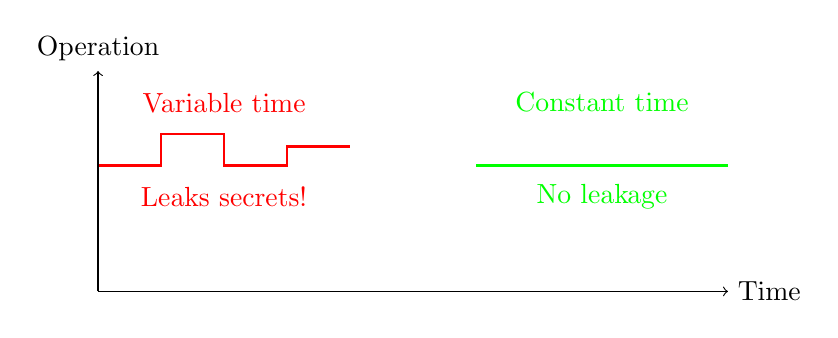
\begin{tikzpicture}[scale=0.8]
    % Variable time
    \draw[thick, red] (0,2) -- (1,2) -- (1,2.5) -- (2,2.5) -- (2,2) -- (3,2) -- (3,2.3) -- (4,2.3);
    \node[red] at (2,3) {Variable time};
    \node[red] at (2,1.5) {Leaks secrets!};
    
    % Constant time
    \draw[thick, green] (6,2) -- (10,2);
    \node[green] at (8,3) {Constant time};
    \node[green] at (8,1.5) {No leakage};
    
    % Time axis
    \draw[->] (0,0) -- (10,0) node[right] {Time};
    \draw[->] (0,0) -- (0,3.5) node[above] {Operation};
\end{tikzpicture}
\caption{Constant-time execution: The same duration regardless of secret values}
\end{figure}

\paragraph{Lattice-Specific Side-Channel Challenges}

Lattice cryptography introduces unique side-channel risks:

\textbf{1. Polynomial Multiplication Timing}
\begin{itemize}
    \item NTT butterflies must be constant-time
    \item Modular reduction after multiplication critical
    \item Cache timing attacks on coefficient access
\end{itemize}

\begin{lstlisting}[language=C, caption=Constant-Time NTT Butterfly]
// SECURE: Constant-time butterfly operation
void butterfly(int16_t *a, int16_t *b, int16_t w) {
    int32_t t = montgomery_multiply(*b, w);
    // No branches, just arithmetic
    *b = *a - t;
    *a = *a + t;
    // Conditional reduction without branches
    *a -= (KYBER_Q & -((*a >= KYBER_Q)));
    *b += (KYBER_Q & -((*b < 0)));
}
\end{lstlisting}

\textbf{2. Rejection Sampling in Signatures}

\begin{algorithm}
\caption{Side-Channel Resistant Rejection Sampling}
\label{alg:ct-rejection}
\begin{algorithmic}[1]
\State \textbf{INSECURE approach:}
\While{$\|\mathbf{z}\|_\infty \geq \gamma - \beta$}
    \State Resample \Comment{Iterations leak secret!}
\EndWhile

\State \textbf{SECURE approach:}
\For{$i = 1$ to MAX\_ATTEMPTS}
    \State Sample candidate
    \State $\text{accept} \gets \text{CT\_Compare}(\|\mathbf{z}\|_\infty, \gamma - \beta)$
    \State $\text{result} \gets \text{CT\_Select}(\text{accept}, \mathbf{z}, \text{result})$
\EndFor
\State \Comment{Always runs MAX\_ATTEMPTS iterations}
\end{algorithmic}
\end{algorithm}

\textbf{3. Error Sampling Leakage}

The discrete Gaussian sampling in lattice schemes is particularly vulnerable:

\begin{figure}[h]
\centering
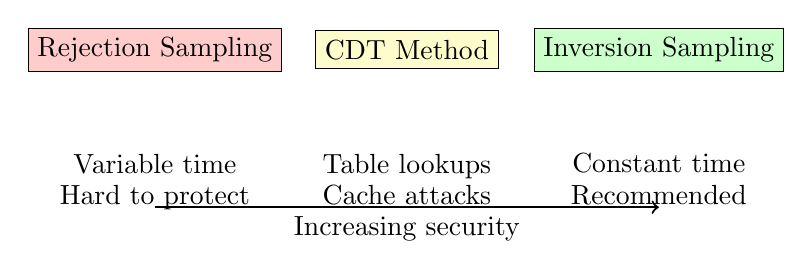
\begin{tikzpicture}[scale=0.8]
    % Gaussian sampling methods
    \node[draw, rectangle, fill=red!20] (rej) at (0,2) {Rejection Sampling};
    \node[draw, rectangle, fill=yellow!20] (cdt) at (4,2) {CDT Method};
    \node[draw, rectangle, fill=green!20] (inv) at (8,2) {Inversion Sampling};
    
    % Properties
    \node[below] at (0,0.5) {Variable time};
    \node[below] at (0,0) {Hard to protect};
    
    \node[below] at (4,0.5) {Table lookups};
    \node[below] at (4,0) {Cache attacks};
    
    \node[below] at (8,0.5) {Constant time};
    \node[below] at (8,0) {Recommended};
    
    % Arrows
    \draw[thick, ->] (0,-0.5) -- (8,-0.5);
    \node[below] at (4,-0.5) {Increasing security};
\end{tikzpicture}
\caption{Gaussian sampling methods: Trade security for efficiency}
\end{figure}

\paragraph{The Falcon Challenge: Floating-Point Side Channels}

Falcon's use of floating-point arithmetic creates unique vulnerabilities:

\begin{itemize}
    \item FP operations have variable timing on many CPUs
    \item Denormalized numbers cause timing variations
    \item Rounding modes affect results
    \item FP exceptions can leak information
\end{itemize}

\begin{example}[FP Timing Attack]
\begin{lstlisting}[language=C]
// Floating-point operations timing depends on values
double gaussian_sample(double sigma, double center) {
    double x = random_double();
    // DANGER: exp() timing varies with input
    double prob = exp(-(x - center)^2 / (2 * sigma^2));
    // DANGER: comparison timing may vary
    if (random_double() < prob) {
        return x;  // Variable number of iterations!
    }
}
\end{lstlisting}
\end{example}

\paragraph{Hardware vs Software Trade-offs}

\begin{table}[h]
\centering
\begin{tabular}{|l|l|l|}
\hline
\textbf{Aspect} & \textbf{Hardware} & \textbf{Software} \\
\hline
Timing control & Excellent & Challenging \\
Power analysis & Vulnerable & Less exposed \\
Cost per algorithm & High & Low \\
Flexibility & Poor & Excellent \\
Performance & Optimal & Good with SIMD \\
Certification & Easier & Harder \\
\hline
\end{tabular}
\caption{Hardware provides better side-channel resistance at higher cost}
\end{table}

\textbf{Recommended approaches:}
\begin{itemize}
    \item \textbf{Hardware:} Custom ASIC/FPGA for high-security applications
    \item \textbf{Software:} Assembly with careful constant-time verification
    \item \textbf{Hybrid:} Hardware RNG + software implementation
\end{itemize}

\subsubsection{Random Number Generation}

Lattice-based cryptography is extraordinarily hungry for randomness. Poor RNG quality doesn't just weaken security—it can completely destroy it.

\paragraph{Why Lattice Crypto Needs More Randomness}

\begin{table}[h]
\centering
\begin{tabular}{|l|c|c|}
\hline
\textbf{Operation} & \textbf{RSA-2048} & \textbf{Kyber-768} \\
\hline
Key generation & 256 bytes & 3,200 bytes \\
Signature & 32 bytes & 4,096 bytes \\
Encryption & 32 bytes & 1,152 bytes \\
\hline
\end{tabular}
\caption{Lattice schemes consume 10-100× more random bytes}
\end{table}

\textbf{What needs randomness:}
\begin{itemize}
    \item Error vectors (thousands of samples)
    \item Ephemeral secrets
    \item Masking values for signatures
    \item Rejection sampling loops
\end{itemize}

\paragraph{Quality Requirements: Not All Randomness is Equal}

\begin{definition}[Cryptographic RNG Requirements]
For lattice-based cryptography, the RNG must provide:
\begin{enumerate}
    \item \textbf{Statistical uniformity:} Indistinguishable from true random
    \item \textbf{Unpredictability:} Cannot predict future outputs
    \item \textbf{Backtracking resistance:} Cannot recover past outputs
    \item \textbf{High throughput:} MB/s for key generation
\end{enumerate}
\end{definition}

\begin{example}[RNG Failure Impact]
Debian OpenSSL disaster (2008) in PQC context:
\begin{itemize}
    \item Weak RNG reduced entropy to 15 bits
    \item For RSA: 32,768 possible keys (bad)
    \item For Kyber: Error distribution destroyed
    \item Result: Linear algebra attack recovers secret instantly
    \item Lesson: Lattice crypto fails catastrophically with bad RNG
\end{itemize}
\end{example}

\paragraph{Gaussian Sampling: The Distribution Challenge}

Most lattice schemes need Gaussian-distributed errors, not uniform:

\begin{algorithm}
\caption{Discrete Gaussian Sampling}
\label{alg:gaussian-sample}
\begin{algorithmic}[1]
\State \textbf{Input:} Standard deviation $\sigma$, center $\mu$
\State \textbf{Output:} Sample from $D_{\mathbb{Z},\sigma,\mu}$

\State \textbf{Method 1: Rejection Sampling}
\While{true}
    \State $x \gets$ UniformInteger($[-\tau\sigma, \tau\sigma]$)
    \State $p \gets \exp(-(x-\mu)^2/(2\sigma^2))$
    \State If UniformReal() $< p$: return $x$
\EndWhile

\State \textbf{Method 2: CDT (Cumulative Distribution Table)}
\State $r \gets$ UniformInteger($[0, 2^{64}-1]$)
\State Binary search CDT for interval containing $r$
\State Return corresponding value

\State \textbf{Method 3: Convolution (Kyber approach)}
\State Sum 2-3 centered binomial samples
\State Approximates Gaussian, constant-time
\end{algorithmic}
\end{algorithm}

\begin{figure}[h]
\centering
\begin{tikzpicture}[scale=0.8]
    % Uniform to Gaussian transformation
    \draw[thick, ->] (0,0) -- (0,3);
    \draw[thick, ->] (0,0) -- (4,0);
    \draw[thick, blue] (0,1.5) -- (4,1.5);
    \node[blue] at (2,2) {Uniform input};
    
    \draw[thick, ->] (5,1.5) -- (6,1.5);
    \node[above] at (5.5,1.5) {Transform};
    
    \draw[thick, ->] (7,0) -- (7,3);
    \draw[thick, ->] (7,0) -- (11,0);
    \draw[thick, red] plot[smooth, domain=7:11] 
        (\x, {2.5*exp(-2*(\x-9)*(\x-9))});
    \node[red] at (9,2.5) {Gaussian output};
\end{tikzpicture}
\caption{RNG challenge: Transform uniform bits to Gaussian distribution}
\end{figure}

\paragraph{Deterministic Variants: Removing RNG Dependence}

Modern PQC often uses deterministic variants to reduce RNG exposure:

\begin{lstlisting}[language=C, caption=Deterministic Key Generation]
// Traditional: Needs continuous RNG
void keygen_random(pk, sk) {
    s = sample_random();      // RNG call
    e = sample_random();      // RNG call
    A = expand_random_seed(); // RNG call
    pk = (A, As + e);
    sk = s;
}

// Deterministic: Single RNG seed
void keygen_deterministic(pk, sk, seed) {
    // Expand single 32-byte seed deterministically
    (seedA, seedS) = SHA3-512(seed);
    A = expand_seed(seedA);
    s = sample_from_seed(seedS, 0);
    e = sample_from_seed(seedS, 1);
    pk = (A, As + e);
    sk = s;
}
\end{lstlisting}

\textbf{Advantages:}
\begin{itemize}
    \item Reproducible key generation
    \item Easier testing and debugging
    \item Less RNG exposure
    \item Enables key recovery from seed
\end{itemize}

\textbf{Risks:}
\begin{itemize}
    \item Seed compromise loses everything
    \item Side-channels on seed expansion
    \item Must protect seed lifetime
\end{itemize}

\subsubsection{Key and Signature Sizes}

The elephant in the room: post-quantum cryptography is big. Understanding the size impact is crucial for system design.

\paragraph{The Stark Reality: Size Comparison}

\begin{table}[h]
\centering
\begin{tabular}{|l|r|r|r|r|}
\hline
\textbf{Algorithm} & \textbf{Public Key} & \textbf{Private Key} & \textbf{Signature} & \textbf{Ciphertext} \\
\hline
\multicolumn{5}{|c|}{\textbf{Current Algorithms}} \\
\hline
RSA-2048 & 256 B & 256 B & 256 B & 256 B \\
RSA-3072 & 384 B & 384 B & 384 B & 384 B \\
ECDSA-P256 & 64 B & 32 B & 64 B & — \\
ECDH-P256 & 64 B & 32 B & — & 64 B \\
Ed25519 & 32 B & 32 B & 64 B & — \\
\hline
\multicolumn{5}{|c|}{\textbf{Post-Quantum Algorithms}} \\
\hline
ML-KEM-768 & 1,184 B & 2,400 B & — & 1,088 B \\
ML-DSA-65 & 1,952 B & 4,032 B & 3,309 B & — \\
Falcon-512 & 897 B & 1,281 B & 666 B & — \\
SPHINCS+-128s & 32 B & 64 B & 7,856 B & — \\
\hline
\multicolumn{5}{|c|}{\textbf{Size Increase Factor}} \\
\hline
ML-KEM vs ECDH & 18.5× & 75× & — & 17× \\
ML-DSA vs Ed25519 & 61× & 126× & 52× & — \\
Falcon vs Ed25519 & 28× & 40× & 10× & — \\
\hline
\end{tabular}
\caption{PQC size explosion: 10-100× larger than current algorithms}
\end{table}

\paragraph{Protocol Impact: Where Size Hurts}

\textbf{1. TLS Handshake Explosion}

\begin{figure}[h]
\centering
\begin{tikzpicture}[scale=0.8]
    % Current TLS
    \draw[thick, fill=blue!20] (0,0) rectangle (2,1);
    \node at (1,0.5) {1.5 KB};
    \node[above] at (1,1) {Current TLS};
    
    % PQC TLS
    \draw[thick, fill=red!20] (4,0) rectangle (10,1);
    \node at (7,0.5) {9 KB};
    \node[above] at (7,1) {PQC TLS};
    
    % Breakdown
    \draw[thick] (0,-1) rectangle (2,-1.5);
    \node[font=\footnotesize] at (1,-1.25) {Certs: 1 KB};
    
    \draw[thick] (4,-1) rectangle (7.5,-1.5);
    \node[font=\footnotesize] at (5.75,-1.25) {Certs: 7 KB};
    
    \draw[thick] (7.5,-1) rectangle (10,-1.5);
    \node[font=\footnotesize] at (8.75,-1.25) {KEM: 2 KB};
\end{tikzpicture}
\caption{TLS handshake size increases 6× with PQC}
\end{figure}

\textbf{2. Certificate Chain Explosion}

\begin{example}[Real Certificate Chain]
Current (RSA-2048):
\begin{itemize}
    \item Root: 1.5 KB (256 B signature)
    \item Intermediate: 1.5 KB (256 B signature)  
    \item Leaf: 1.5 KB (256 B signature)
    \item Total: 4.5 KB
\end{itemize}

With ML-DSA-65:
\begin{itemize}
    \item Root: 4.8 KB (3.3 KB signature)
    \item Intermediate: 4.8 KB (3.3 KB signature)
    \item Leaf: 4.8 KB (3.3 KB signature)
    \item Total: 14.4 KB (3.2× increase)
\end{itemize}
\end{example}

\textbf{3. IoT and Embedded Systems}

\begin{table}[h]
\centering
\begin{tabular}{|l|c|c|c|}
\hline
\textbf{Constraint} & \textbf{Typical IoT} & \textbf{ML-KEM-768} & \textbf{Feasible?} \\
\hline
Flash (code) & 256 KB & +40 KB & Maybe \\
RAM (runtime) & 32 KB & 8 KB & Yes \\
Key storage & 4 KB & 3.6 KB & Tight \\
Bandwidth & 250 kbps & 9 KB handshake & Challenging \\
Battery (per op) & 1 mJ & 0.5 mJ & Yes \\
\hline
\end{tabular}
\caption{PQC on constrained devices: Possible but challenging}
\end{table}

\paragraph{Storage and Bandwidth Considerations}

\textbf{Database Impact:}
\begin{itemize}
    \item User authentication DB with 1M users
    \item Current (Ed25519): 32 MB public keys
    \item PQC (ML-DSA): 1.95 GB public keys
    \item 61× storage increase
\end{itemize}

\textbf{Network Impact:}
\begin{itemize}
    \item Mobile app checking 100 signatures/day
    \item Current: 6.4 KB/day
    \item PQC: 331 KB/day
    \item Monthly: 10 MB extra data usage
\end{itemize}

\textbf{Blockchain Catastrophe:}
\begin{itemize}
    \item Bitcoin transaction: ~250 bytes
    \item With PQC signatures: ~3,500 bytes
    \item Blockchain size growth: 14× faster
    \item Full node storage: TB → 14 TB
\end{itemize}

\paragraph{Mitigation Strategies}

\textbf{1. Compression Techniques}
\begin{itemize}
    \item Compress public keys when storing
    \item Use seed + expansion for deterministic keys
    \item Domain separation for multiple keys
    \item Typical savings: 20-30\%
\end{itemize}

\textbf{2. Hybrid Modes During Transition}
\begin{lstlisting}[language=C, caption=Size-Optimized Hybrid Mode]
// Naive hybrid: RSA + PQC (size = both)
struct hybrid_sig_naive {
    uint8_t rsa_sig[256];
    uint8_t pqc_sig[3309];
}; // Total: 3,565 bytes

// Optimized: Sign hash with both
struct hybrid_sig_opt {
    uint8_t data_hash[32];
    uint8_t rsa_sig[256];
    uint8_t pqc_sig[666];  // Use Falcon
}; // Total: 954 bytes
\end{lstlisting}

\textbf{3. Protocol Adaptations}
\begin{itemize}
    \item Cache certificates aggressively
    \item Use session resumption in TLS
    \item Batch signature verification
    \item Consider SPHINCS+ only for root CAs
\end{itemize}

\begin{remark}[The Size Reality Check]
The size increase is real and painful. No clever optimization makes PQC as small as ECC. Success requires:
\begin{itemize}
    \item Accepting the size increase as necessary
    \item Architecting systems to minimize impact
    \item Using the right algorithm for each use case
    \item Planning infrastructure upgrades early
\end{itemize}
The alternative—broken cryptography—is worse than larger keys.
\end{remark}

\begin{example}[Success Story: Cloudflare's Deployment]
Cloudflare successfully deployed PQC to millions of websites:
\begin{itemize}
    \item Hybrid mode: ECDH + Kyber
    \item Increased handshake: 1.2 KB → 2.9 KB
    \item Performance impact: <0.1 ms
    \item User experience: Unchanged
    \item Lesson: Size increase manageable with good engineering
\end{itemize}
\end{example}

The implementation challenges are real but surmountable. Side-channel protection requires expertise and careful coding. Random number generation needs more attention than ever. And yes, keys and signatures are much larger. But with proper engineering, post-quantum cryptography is deployable today. The next section examines migration strategies to make this transition successful.

\subsection{Migration Strategies}
\label{sec:migration}

The post-quantum migration represents the largest cryptographic transition in history. Every encrypted connection, every digital signature, every authentication protocol must change. Unlike previous migrations that affected specific algorithms, this touches everything using public-key cryptography. The challenge isn't just technical—it's organizational, economic, and urgent. Organizations that start now will transition smoothly. Those that wait risk catastrophic exposure when quantum computers arrive.

\subsubsection{Hybrid Modes}

The safest path to post-quantum security runs through hybrid cryptography: using both classical and post-quantum algorithms together. This isn't overcaution—it's learning from history.

\paragraph{Why Hybrid? Learning from Dual EC DRBG}

\begin{example}[The Cautionary Tale]
Dual EC DRBG (2006-2013):
\begin{itemize}
    \item NSA-designed random number generator
    \item Based on elliptic curves (considered secure)
    \item Standardized by NIST
    \item Later revealed: Deliberate backdoor
    \item Lesson: Even standardized algorithms can fail
\end{itemize}
\end{example}

Hybrid modes protect against:
\begin{itemize}
    \item \textbf{Classical breaks:} If PQC algorithm broken classically
    \item \textbf{Implementation flaws:} Bugs in new PQC code
    \item \textbf{Quantum timeline uncertainty:} If quantum computers arrive early
    \item \textbf{Standard changes:} If NIST updates algorithms
\end{itemize}

\paragraph{Hybrid Construction Methods}

\textbf{Method 1: Concatenation (Simple but Large)}

\begin{algorithm}
\caption{Hybrid Key Exchange - Concatenation}
\label{alg:hybrid-concat}
\begin{algorithmic}[1]
\State \textbf{Client:}
\State \quad Generate $(pk_{ecc}, sk_{ecc}) \leftarrow$ ECDH.KeyGen()
\State \quad Generate $(pk_{pqc}, sk_{pqc}) \leftarrow$ Kyber.KeyGen()
\State \quad Send $(pk_{ecc}, pk_{pqc})$ to server

\State \textbf{Server:}
\State \quad $K_{ecc} \leftarrow$ ECDH.Encapsulate($pk_{ecc}$)
\State \quad $(c_{pqc}, K_{pqc}) \leftarrow$ Kyber.Encapsulate($pk_{pqc}$)
\State \quad $K_{final} = \text{KDF}(K_{ecc} || K_{pqc})$
\State \quad Send $(c_{ecc}, c_{pqc})$ to client

\State \textbf{Security:} Must break BOTH to get $K_{final}$
\end{algorithmic}
\end{algorithm}

\textbf{Method 2: Nested (Better Integration)}

\begin{figure}[h]
\centering
\begin{tikzpicture}[scale=0.8]
    % Nested encryption
    \node[draw, rectangle, minimum width=6cm, minimum height=1cm] (msg) at (0,0) {Message};
    
    \draw[thick, blue] (-3.5,-0.8) rectangle (3.5,0.8);
    \node[blue] at (4.5,0) {PQC Layer};
    
    \draw[thick, red] (-4.2,-1.5) rectangle (4.2,1.5);
    \node[red] at (5.2,0) {Classical Layer};
    
    % Arrows
    \draw[->, thick] (0,-2.5) -- (0,-3.5);
    \node[below] at (0,-3.5) {Double protection};
    
    % Attack scenarios
    \node[align=left] at (8,0) {
        Break classical only: PQC protects\\
        Break PQC only: Classical protects\\
        Must break both: Infeasible
    };
\end{tikzpicture}
\caption{Nested hybrid: Each layer independently protects the data}
\end{figure}

\paragraph{Security Analysis of Hybrid Modes}

\begin{theorem}[Hybrid Security]
For hybrid scheme $H = (C, P)$ combining classical $C$ and post-quantum $P$:
\begin{itemize}
    \item If $C$ is $(t_c, \epsilon_c)$-secure and $P$ is $(t_p, \epsilon_p)$-secure
    \item Then $H$ is $(t, \epsilon)$-secure where:
    \item $t = \min(t_c, t_p)$ and $\epsilon \leq \epsilon_c + \epsilon_p$
\end{itemize}
\end{theorem}

\textbf{Real security levels:}

\begin{table}[h]
\centering
\begin{tabular}{|l|c|c|c|}
\hline
\textbf{Configuration} & \textbf{Classical} & \textbf{Quantum} & \textbf{Confidence} \\
\hline
ECDH-P256 only & 128-bit & 0-bit & High \\
Kyber-768 only & 180-bit & 128-bit & Medium \\
Hybrid both & 128-bit & 128-bit & Highest \\
\hline
\end{tabular}
\caption{Hybrid provides quantum resistance without sacrificing classical security}
\end{table}

\paragraph{Performance Impact}

The cost of hybrid modes:

\begin{table}[h]
\centering
\begin{tabular}{|l|r|r|r|r|}
\hline
\textbf{Operation} & \textbf{ECDH} & \textbf{Kyber} & \textbf{Hybrid} & \textbf{Overhead} \\
\hline
Key generation & 45 µs & 35 µs & 80 µs & 1.78× \\
Encapsulation & 45 µs & 44 µs & 89 µs & 1.98× \\
Decapsulation & 45 µs & 40 µs & 85 µs & 1.89× \\
Handshake size & 96 B & 2,272 B & 2,368 B & 24.7× \\
\hline
\end{tabular}
\caption{Hybrid overhead: ~2× time, dominated by PQC size}
\end{table}

\begin{example}[Google's CECPQ2 Experiment]
Google tested hybrid ECDH+NTRU in Chrome (2019):
\begin{itemize}
    \item 30\% of TLS connections used hybrid
    \item Median latency increase: 1 ms
    \item 95th percentile: 20 ms increase
    \item User complaints: Zero
    \item Conclusion: Hybrid deployment feasible at scale
\end{itemize}
\end{example}

\subsubsection{Timeline and Urgency}

The quantum threat creates an unprecedented situation: we must protect against computers that don't yet exist. Understanding the timeline is crucial for appropriate urgency.

\paragraph{The Quantum Timeline: Best Estimates}

\begin{figure}[h]
\centering
\begin{tikzpicture}[scale=0.9]
    % Timeline
    \draw[thick, ->] (0,0) -- (12,0);
    \foreach \x/\year in {0/2024, 2/2028, 4/2032, 6/2036, 8/2040, 10/2044} {
        \draw[thick] (\x,0.1) -- (\x,-0.1);
        \node[below] at (\x,-0.2) {\year};
    }
    
    % Quantum development
    \draw[thick, red] plot[smooth] coordinates {
        (0,1) (1,1.3) (2,1.7) (3,2.2) (4,2.8) (5,3.5) (6,4.3) (7,5.2) (8,6.2)
    };
    \node[red, right] at (8,6.2) {Quantum capability};
    
    % Threat levels
    \draw[dashed, green] (0,2) -- (12,2);
    \node[green, right] at (12,2) {Break ECC-256};
    
    \draw[dashed, orange] (0,4) -- (12,4);
    \node[orange, right] at (12,4) {Break RSA-2048};
    
    \draw[dashed, red] (0,6) -- (12,6);
    \node[red, right] at (12,6) {Break everything};
    
    % Key events
    \draw[thick, blue, <->] (0,7) -- (4,7);
    \node[blue, above] at (2,7) {Migration window};
    
    \draw[thick, purple] (4,0) -- (4,8);
    \node[purple, above] at (4,8) {Too late to start};
\end{tikzpicture}
\caption{Quantum timeline: Migration must complete before quantum computers arrive}
\end{figure}

\textbf{Expert predictions (2024):}
\begin{itemize}
    \item \textbf{Optimistic:} Cryptographically relevant QC by 2030
    \item \textbf{Realistic:} 2035-2040 for RSA-2048 threats
    \item \textbf{Conservative:} 2040-2050 for large-scale breaks
    \item \textbf{IBM Roadmap:} 100,000 qubits by 2033
\end{itemize}

\paragraph{Why Start Now? The Mosaic Theory}

\begin{definition}[Mosaic Theory of Migration]
Cryptographic migration isn't one project—it's thousands of interconnected changes that must happen in sequence:
\begin{itemize}
    \item Standards must finalize (2024) \checkmark
    \item Libraries must implement (2024-2025)
    \item Products must integrate (2025-2027)
    \item Deployments must complete (2027-2030)
    \item Legacy must sunset (2030-2035)
\end{itemize}
\end{definition}

\begin{example}[The 10-Year Rule]
SHA-1 deprecation timeline:
\begin{itemize}
    \item 2005: First collision attacks published
    \item 2014: Chrome starts warning
    \item 2017: First practical collision
    \item 2020: Windows stops SHA-1 support
    \item 2024: Still found in legacy systems
    \item Total: 19 years and counting!
\end{itemize}
PQC migration is 100× more complex.
\end{example}

\paragraph{Lessons from Previous Migrations}

\textbf{Success: AES Adoption}
\begin{itemize}
    \item Clear deadline: DES key too small
    \item Drop-in replacement: Same interface
    \item Performance gain: AES faster than 3DES
    \item Result: Smooth transition
\end{itemize}

\textbf{Failure: IPv6 Adoption}
\begin{itemize}
    \item No hard deadline
    \item Requires infrastructure changes
    \item No immediate benefit
    \item Result: 25 years, still incomplete
\end{itemize}

\textbf{PQC resembles IPv6 more than AES:}
\begin{itemize}
    \item No immediate threat visible
    \item Requires protocol changes
    \item Performance degradation
    \item Risk: Similar 20+ year transition
\end{itemize}

\paragraph{Risk Assessment: The "Harvest Now, Decrypt Later" Reality}

\begin{table}[h]
\centering
\begin{tabular}{|l|c|c|c|}
\hline
\textbf{Data Type} & \textbf{Lifetime} & \textbf{Risk Level} & \textbf{Action Needed} \\
\hline
Government secrets & 25-50 years & Critical & Immediate \\
Healthcare records & 100 years & Critical & Immediate \\
Financial records & 7-10 years & High & By 2025 \\
IP/Trade secrets & 20 years & High & By 2025 \\
Personal data & Lifetime & Medium & By 2027 \\
Session keys & Hours & Low & By 2030 \\
\hline
\end{tabular}
\caption{Data lifetime determines migration urgency}
\end{table}

\begin{remark}[The Uncomfortable Truth]
If your data needs protection beyond 2035, it's already at risk. Adversaries are likely harvesting encrypted data today for future decryption. Every day of delay is another day of data exposed to future quantum attack.
\end{remark}

\subsubsection{Practical Steps}

Here's your migration playbook—concrete steps every organization should take.

\paragraph{Step 1: Cryptographic Inventory}

You can't protect what you don't know exists.

\begin{algorithm}
\caption{Crypto Discovery Process}
\label{alg:crypto-discovery}
\begin{algorithmic}[1]
\State \textbf{Phase 1: Automated Discovery}
\State \quad Scan codebases for crypto libraries
\State \quad Analyze network traffic for TLS/SSH
\State \quad Check certificates and key stores
\State \quad Inventory hardware security modules

\State \textbf{Phase 2: Manual Review}
\State \quad Interview development teams
\State \quad Review security architecture
\State \quad Check third-party dependencies
\State \quad Document custom implementations

\State \textbf{Phase 3: Risk Classification}
\State \quad Map algorithms to use cases
\State \quad Identify quantum-vulnerable components
\State \quad Prioritize by data sensitivity
\State \quad Create migration roadmap
\end{algorithmic}
\end{algorithm}

\begin{example}[Typical Enterprise Discovery]
Medium enterprise (5,000 employees) crypto inventory:
\begin{itemize}
    \item 2,847 TLS certificates (RSA/ECDSA)
    \item 156 code signing certificates
    \item 89 internal applications using crypto
    \item 1,293 API keys (various algorithms)
    \item 23 different crypto libraries
    \item 7 hardware security modules
    \item Surprise: 45\% unknown to security team!
\end{itemize}
\end{example}

\paragraph{Step 2: Testing Methodology}

\textbf{Test Environment Setup:}

\begin{lstlisting}[language=bash, caption=PQC Testing Framework]
# Create isolated test environment
docker network create pqc-test

# Run PQC-enabled server
docker run -d --name pqc-server \
  --network pqc-test \
  -e CRYPTO_MODE=hybrid \
  -e PQC_ALGO=kyber768 \
  pqc-test-server:latest

# Test client compatibility
for client in legacy current pqc-enabled; do
  docker run --rm --network pqc-test \
    pqc-test-client:$client \
    --target pqc-server \
    --measure-performance
done
\end{lstlisting}

\textbf{Key Testing Areas:}
\begin{enumerate}
    \item \textbf{Functionality:} Do connections succeed?
    \item \textbf{Performance:} Latency and throughput impact
    \item \textbf{Compatibility:} Legacy system interactions
    \item \textbf{Scalability:} Load testing with larger keys
    \item \textbf{Failure modes:} Graceful degradation
\end{enumerate}

\paragraph{Step 3: Rollout Strategies}

\textbf{Strategy 1: Canary Deployment}

\begin{figure}[h]
\centering
\begin{tikzpicture}[scale=0.8]
    % Timeline
    \draw[thick, ->] (0,0) -- (10,0);
    
    % Phases
    \draw[fill=green!20] (0,0.5) rectangle (2,1.5);
    \node at (1,1) {1\% traffic};
    
    \draw[fill=yellow!20] (2,0.5) rectangle (4,1.5);
    \node at (3,1) {10\% traffic};
    
    \draw[fill=orange!20] (4,0.5) rectangle (6,1.5);
    \node at (5,1) {50\% traffic};
    
    \draw[fill=red!20] (6,0.5) rectangle (8,1.5);
    \node at (7,1) {100\% traffic};
    
    % Monitoring
    \node[above] at (5,2) {Continuous monitoring};
    \draw[<->] (0,1.8) -- (8,1.8);
    
    % Rollback
    \draw[->, dashed, blue] (3,0.3) -- (1,0.3);
    \node[below, blue] at (2,0) {Rollback};
\end{tikzpicture}
\caption{Canary deployment: Gradual rollout with monitoring}
\end{figure}

\textbf{Strategy 2: Service-Based Migration}

\begin{itemize}
    \item \textbf{Phase 1:} Internal services (low risk)
    \item \textbf{Phase 2:} B2B connections (controlled)
    \item \textbf{Phase 3:} Customer-facing (careful)
    \item \textbf{Phase 4:} Legacy integration (complex)
\end{itemize}

\paragraph{Step 4: Building Crypto-Agility}

The future demands systems that can change algorithms without redesign.

\begin{definition}[Crypto-Agility]
The ability to rapidly transition between cryptographic algorithms without:
\begin{itemize}
    \item Changing application code
    \item Disrupting service
    \item Breaking compatibility
    \item Manual intervention
\end{itemize}
\end{definition}

\begin{lstlisting}[language=C, caption=Crypto-Agile Design Pattern]
// BAD: Algorithm-specific code
void encrypt_data_rsa(data, rsa_key) { ... }
void encrypt_data_kyber(data, kyber_key) { ... }

// GOOD: Algorithm-agnostic interface
typedef struct {
    enum { RSA, ECDH, KYBER, HYBRID } type;
    void *key;
    size_t key_len;
} crypto_key_t;

void encrypt_data(data, crypto_key_t *key) {
    switch(key->type) {
        case RSA: return rsa_encrypt(data, key);
        case KYBER: return kyber_encrypt(data, key);
        case HYBRID: return hybrid_encrypt(data, key);
    }
}

// Configuration-driven selection
key_type = config_get("crypto.algorithm");
\end{lstlisting}

\textbf{Crypto-Agility Checklist:}
\begin{itemize}
    \item \checkmark Algorithms identified by OIDs, not hardcoded
    \item \checkmark Key sizes parameterized
    \item \checkmark Protocol negotiation supported
    \item \checkmark Multiple algorithms co-exist
    \item \checkmark Monitoring for algorithm usage
    \item \checkmark Automated rollback capability
\end{itemize}

\paragraph{Migration Timeline Template}

\begin{table}[h]
\centering
\begin{tabular}{|l|l|l|}
\hline
\textbf{Year} & \textbf{Milestone} & \textbf{Actions} \\
\hline
2024 & Foundation & Inventory, team training, pilot projects \\
2025 & Implementation & Deploy hybrid modes, update libraries \\
2026 & Expansion & Customer-facing systems, partner integration \\
2027 & Acceleration & Legacy migration, full hybrid deployment \\
2028 & Transition & Begin disabling classical-only modes \\
2029 & Hardening & PQC-only for sensitive data \\
2030 & Completion & Quantum-safe across organization \\
\hline
\end{tabular}
\caption{Seven-year migration: Aggressive but achievable}
\end{table}

\begin{remark}[The Migration Imperative]
Post-quantum migration isn't optional—it's existential. Organizations that complete migration will survive the quantum era. Those that don't face catastrophic exposure. The technical challenges are solvable. The timeline is tight but achievable. The only unforgivable mistake is waiting to start.
\end{remark}

\begin{example}[Success Story: Cloudflare's Leadership]
Cloudflare deployed PQC to 20+ million websites:
\begin{itemize}
    \item Started: 2019 (before standards!)
    \item Hybrid deployment: 2022
    \item Full coverage: 2023
    \item Customer impact: Minimal
    \item Lesson: Early movers gain experience and confidence
\end{itemize}
\end{example}

The migration challenge is real but manageable. Hybrid modes provide safety during transition. The timeline demands urgency without panic. And concrete steps turn an overwhelming challenge into executable projects. The next section examines real-world deployments to learn from early adopters.

\subsection{Real-World Case Studies}
\label{sec:case-studies}

Theory meets reality when post-quantum cryptography deploys at scale. These case studies document real organizations implementing PQC in production, the challenges they faced, and the solutions they found. The message is clear: deployment is harder than expected but entirely feasible. Early adopters are blazing trails that others can follow.

\subsubsection{TLS Migration}

The most visible PQC deployment happens in web browsers and servers. With billions of HTTPS connections daily, TLS migration serves as the canary in the coal mine for post-quantum deployment.

\paragraph{Cloudflare: PQC at Internet Scale}

Cloudflare protects 20+ million websites, making their PQC deployment the largest to date.

\textbf{Deployment Timeline:}
\begin{itemize}
    \item 2019: Initial experiments with CECPQ2 (NTRU-based)
    \item 2021: Switch to Kyber testing
    \item 2022: Hybrid X25519+Kyber768 deployed
    \item 2023: Available to all customers
    \item 2024: 30\% of connections use PQC
\end{itemize}

\textbf{Protocol Changes Required:}

\begin{figure}[h]
\centering
\begin{tikzpicture}[scale=0.8]
    % TLS 1.3 handshake flow
    \node[draw, circle] (client) at (0,0) {Client};
    \node[draw, circle] (server) at (8,0) {Server};
    
    % ClientHello
    \draw[thick, ->] (0,-1) -- (8,-1);
    \node[above] at (4,-1) {ClientHello};
    \node[below, red] at (4,-1) {+2KB for Kyber};
    
    % ServerHello
    \draw[thick, ->] (8,-2.5) -- (0,-2.5);
    \node[above] at (4,-2.5) {ServerHello + Certificate};
    \node[below, red] at (4,-2.5) {+8KB for PQC certs};
    
    % Finished
    \draw[thick, ->] (0,-4) -- (8,-4);
    \node[above] at (4,-4) {Finished};
    
    % Size comparison
    \node[align=left] at (10,-1) {Classical: 1.5KB total};
    \node[align=left, red] at (10,-2) {PQC: 12KB total};
    \node[align=left, red] at (10,-3) {8× increase};
\end{tikzpicture}
\caption{TLS handshake size explosion with PQC}
\end{figure}

\textbf{Implementation Challenges:}

\begin{lstlisting}[language=Go, caption=TLS Library Modifications]
// Before: Fixed-size key shares
type KeyShare struct {
    Group CurveID
    Data  [32]byte  // Works for X25519
}

// After: Variable-size for PQC
type KeyShare struct {
    Group NamedGroup
    Data  []byte    // Now handles 1KB+ Kyber shares
}

// Buffer size increases needed throughout:
const maxHandshakeSize = 65536  // Was 16384
const maxCertChainSize = 32768  // Was 8192
\end{lstlisting}

\paragraph{Certificate Size Impact: The Reality}

\begin{table}[h]
\centering
\begin{tabular}{|l|r|r|r|}
\hline
\textbf{Certificate Component} & \textbf{RSA-2048} & \textbf{Dilithium3} & \textbf{Increase} \\
\hline
Subject info & 200 B & 200 B & 1× \\
Public key & 294 B & 1,952 B & 6.6× \\
CA signature & 256 B & 3,293 B & 12.9× \\
Extensions & 300 B & 300 B & 1× \\
\hline
\textbf{Total certificate} & 1,050 B & 5,745 B & 5.5× \\
\textbf{3-cert chain} & 3,150 B & 17,235 B & 5.5× \\
\hline
\end{tabular}
\caption{Certificate chains dominate PQC handshake overhead}
\end{table}

\textbf{Real measurement from Cloudflare:}
\begin{itemize}
    \item Median handshake time increase: 1.3 ms
    \item 95th percentile: 21 ms increase
    \item 99th percentile: 87 ms increase
    \item Mobile impact: 2-3× larger than desktop
\end{itemize}

\paragraph{Performance Measurements in Production}

\begin{figure}[h]
\centering
\begin{tikzpicture}[scale=0.8]
    % Performance graph
    \draw[->] (0,0) -- (10,0) node[right] {Connections/sec};
    \draw[->] (0,0) -- (0,6) node[above] {CPU Usage (\%)};
    
    % Data points
    \draw[thick, blue] plot coordinates {
        (0,1) (2,1.2) (4,1.8) (6,2.8) (8,4.2) (10,5.5)
    };
    \node[blue] at (8,5) {ECDHE};
    
    \draw[thick, red] plot coordinates {
        (0,1.2) (2,1.5) (4,2.3) (6,3.5) (8,5.1) (10,6.5)
    };
    \node[red] at (8,6) {Kyber768};
    
    \draw[thick, green] plot coordinates {
        (0,1.3) (2,1.7) (4,2.6) (6,4.0) (8,5.8) (10,7.5)
    };
    \node[green] at (7,7) {Hybrid};
    
    % Annotations
    \draw[dashed] (5,0) -- (5,6);
    \node[below] at (5,0) {50K conn/s};
    \node at (5,5) {+40\% CPU};
\end{tikzpicture}
\caption{CPU overhead: Manageable but noticeable at scale}
\end{figure}

\paragraph{Lessons Learned from TLS Deployment}

\begin{enumerate}
    \item \textbf{Buffer sizes:} Every buffer in the stack needs expansion
    \item \textbf{MTU issues:} Large certificates trigger fragmentation
    \item \textbf{Middleboxes:} Some corporate firewalls reject large TLS messages
    \item \textbf{Client diversity:} Embedded clients often have fixed buffers
    \item \textbf{Caching critical:} Session resumption more important than ever
\end{enumerate}

\begin{example}[The Middlebox Problem]
A major bank's PQC pilot failed mysteriously:
\begin{itemize}
    \item Symptom: 15\% of connections dropped
    \item Investigation: 6 weeks of debugging
    \item Root cause: Corporate firewall had 8KB TLS message limit
    \item PQC certificates: 12KB
    \item Solution: Fragment certificates across multiple TLS records
    \item Lesson: Infrastructure has hidden assumptions
\end{itemize}
\end{example}

\subsubsection{Code Signing}

Code signing presents unique challenges: signatures are stored forever, backward compatibility is crucial, and size directly impacts distribution.

\paragraph{Microsoft's Windows Update Challenge}

Windows Update serves billions of devices, making signature size critical.

\textbf{Current State:}
\begin{itemize}
    \item 2+ billion Windows devices
    \item Updates signed with RSA-2048 + SHA-256
    \item Signature size: 256 bytes per file
    \item Typical update: 1,000-10,000 signed files
\end{itemize}

\textbf{PQC Impact Analysis:}
\begin{table}[h]
\centering
\begin{tabular}{|l|r|r|r|}
\hline
\textbf{Metric} & \textbf{Current} & \textbf{With Dilithium3} & \textbf{Impact} \\
\hline
Signature per file & 256 B & 3,293 B & 12.9× \\
Update metadata & 256 KB & 3.3 MB & 12.9× \\
Download increase & — & +3 MB & Per update \\
Verification time & 0.5 ms & 0.4 ms & Faster! \\
\hline
\end{tabular}
\caption{Code signing: Size hurts more than performance}
\end{table}

\textbf{Microsoft's Hybrid Approach:}

\begin{lstlisting}[language=C, caption=Dual-Signature Format]
typedef struct {
    // Traditional signature for compatibility
    BYTE RSASignature[256];
    
    // PQC signature in extension
    struct {
        DWORD dwMagic;  // 'PQCS'
        WORD  wAlgId;   // DILITHIUM3
        WORD  wSigLen;  // 3293
        BYTE  PQCSignature[3293];
    } PQCExtension;
} DUAL_SIGNATURE;

// Verification logic
BOOL VerifyCodeSignature(file, signature) {
    if (SystemSupportsPQC()) {
        return VerifyPQC(file, signature.PQCExtension);
    } else {
        return VerifyRSA(file, signature.RSASignature);
    }
}
\end{lstlisting}

\paragraph{Backwards Compatibility Strategies}

\textbf{Strategy 1: Append PQC Signatures}
\begin{itemize}
    \item Old systems ignore unknown data
    \item New systems check both signatures
    \item File size increases significantly
    \item Works for most formats
\end{itemize}

\textbf{Strategy 2: Dual Signing Infrastructure}
\begin{itemize}
    \item Maintain two separate signature systems
    \item Serve appropriate version based on client
    \item Complex infrastructure
    \item Enables gradual transition
\end{itemize}

\textbf{Strategy 3: Signature Stripping}
\begin{itemize}
    \item Store PQC signatures separately
    \item Strip for legacy clients
    \item Reduces bandwidth for old systems
    \item Requires proxy infrastructure
\end{itemize}

\paragraph{Apple's Approach: Preparing the Ecosystem}

Apple's strategy focuses on ecosystem preparation:

\begin{enumerate}
    \item \textbf{2023:} Added PQC algorithms to Security.framework
    \item \textbf{2024:} Developer tools support hybrid signing
    \item \textbf{2025:} App Store accepts PQC-signed apps
    \item \textbf{2026:} New devices require PQC signatures
    \item \textbf{2028:} Legacy signature support deprecated
\end{enumerate}

\begin{example}[Real App Impact]
Popular iOS app (100MB) with PQC signatures:
\begin{itemize}
    \item Current: 487 signed components
    \item RSA signatures: 125 KB total
    \item Dilithium signatures: 1.6 MB total
    \item App size increase: 1.5\%
    \item User impact: Negligible
    \item Developer impact: Toolchain updates needed
\end{itemize}
\end{example}

\subsubsection{Blockchain and Cryptocurrencies}

Blockchain faces the perfect storm: immutable history, size-sensitive economics, and catastrophic failure modes. The challenges are so severe that some blockchains may not survive the transition.

\paragraph{Bitcoin's Existential Crisis}

Bitcoin faces unique challenges that make PQC migration extraordinarily difficult:

\textbf{The Immutability Problem:}
\begin{itemize}
    \item 800+ million historical transactions
    \item All use ECDSA signatures (vulnerable)
    \item Blockchain is immutable by design
    \item Old signatures must remain verifiable
    \item But quantum computers can forge them!
\end{itemize}

\begin{figure}[h]
\centering
\begin{tikzpicture}[scale=0.8]
    % Blockchain
    \draw[thick] (0,0) rectangle (2,1);
    \node at (1,0.5) {Block 1};
    \draw[thick] (2,0) rectangle (4,1);
    \node at (3,0.5) {Block 2};
    \draw[thick] (4,0) rectangle (6,1);
    \node at (5,0.5) {...};
    \draw[thick] (6,0) rectangle (8,1);
    \node at (7,0.5) {Block N};
    
    % Signatures
    \node[red] at (1,-0.5) {ECDSA};
    \node[red] at (3,-0.5) {ECDSA};
    \node[red] at (7,-0.5) {ECDSA};
    
    % Quantum attack
    \draw[thick, red, ->] (4,-2) -- (4,-1);
    \node[red] at (4,-2.5) {Quantum attacker};
    \node[red] at (4,-3) {Can forge any signature!};
    
    % Problem
    \node[align=center] at (4,2) {Cannot change past blocks\\Cannot invalidate old signatures\\Cannot prevent forgery};
\end{tikzpicture}
\caption{Blockchain's immutability makes PQC migration nearly impossible}
\end{figure}

\paragraph{Transaction Size Explosion}

\begin{table}[h]
\centering
\begin{tabular}{|l|r|r|r|}
\hline
\textbf{Transaction Type} & \textbf{Current} & \textbf{With PQC} & \textbf{Factor} \\
\hline
Simple transfer & 250 B & 3,500 B & 14× \\
Multisig (2-of-3) & 370 B & 10,200 B & 27.6× \\
Smart contract call & 500 B & 7,000 B & 14× \\
\hline
\textbf{Block capacity} & 4,000 tx & 285 tx & 0.07× \\
\textbf{Fees (est.)} & \$2 & \$28 & 14× \\
\hline
\end{tabular}
\caption{PQC destroys blockchain economics}
\end{table}

\textbf{Network impact:}
\begin{itemize}
    \item Current throughput: 7 tx/sec
    \item With PQC: 0.5 tx/sec
    \item Blockchain growth: 50 GB/year → 700 GB/year
    \item Full node storage: 500 GB → 7 TB
    \item Sync time: Days → Months
\end{itemize}

\paragraph{Ethereum's Migration Strategy}

Ethereum, being more flexible, has better options:

\begin{algorithm}
\caption{Ethereum's Planned PQC Migration}
\label{alg:eth-pqc}
\begin{algorithmic}[1]
\State \textbf{Phase 1: Account Abstraction} (2024-2025)
\State \quad Enable smart contract wallets
\State \quad Support multiple signature types
\State \quad Deploy PQC-capable contracts

\State \textbf{Phase 2: Hybrid Period} (2025-2027)
\State \quad New accounts use PQC
\State \quad Old accounts can migrate
\State \quad Both signature types valid

\State \textbf{Phase 3: Incentivized Migration} (2027-2029)
\State \quad Reduced gas for PQC transactions
\State \quad Higher fees for ECDSA
\State \quad Automated migration tools

\State \textbf{Phase 4: Quantum-Safe} (2030+)
\State \quad Disable ECDSA for new transactions
\State \quad Historical validation remains
\State \quad State commitments use PQC
\end{algorithmic}
\end{algorithm}

\paragraph{The Fork Dilemma}

Some blockchains may need hard forks:

\begin{figure}[h]
\centering
\begin{tikzpicture}[scale=0.8]
    % Original chain
    \draw[thick] (0,0) -- (4,0);
    \node[above] at (2,0) {Original chain};
    
    % Fork point
    \draw[fill=red] (4,0) circle (3pt);
    \node[above] at (4,0.3) {Fork};
    
    % Two chains
    \draw[thick] (4,0) -- (8,1);
    \node[above] at (6,1) {PQC chain};
    
    \draw[thick, dashed] (4,0) -- (8,-1);
    \node[below] at (6,-1) {Legacy chain};
    
    % Annotations
    \node[align=left] at (10,1) {New rules\\PQC only\\Smaller community};
    \node[align=left] at (10,-1) {Old rules\\Quantum vulnerable\\May die};
\end{tikzpicture}
\caption{Hard fork: The nuclear option for blockchain PQC migration}
\end{figure}

\paragraph{Novel Solutions Being Explored}

\textbf{1. Stateless Clients with PQC}
\begin{itemize}
    \item Don't store full blockchain
    \item Verify using cryptographic proofs
    \item Proofs can use PQC
    \item Reduces storage burden
\end{itemize}

\textbf{2. Commit-Reveal Schemes}
\begin{itemize}
    \item Commit to address hash now
    \item Reveal PQC public key when spending
    \item Protects unspent outputs
    \item Requires protocol changes
\end{itemize}

\textbf{3. Quantum-Safe Sidechains}
\begin{itemize}
    \item Create parallel PQC blockchain
    \item Bridge assets between chains
    \item Gradual value migration
    \item Original chain can die gracefully
\end{itemize}

\begin{example}[Zcash's Approach]
Zcash plans the most aggressive migration:
\begin{itemize}
    \item Already supports multiple address types
    \item Will add PQC addresses alongside existing
    \item Turnstile migration: Must move funds to new address
    \item Old addresses deprecated after transition
    \item Estimated timeline: 5 years
    \item User impact: Must actively migrate or lose funds
\end{itemize}
\end{example}

\paragraph{Lessons from Blockchain Challenges}

\begin{enumerate}
    \item \textbf{Immutability $\neq$ Security:} Cannot fix past mistakes
    \item \textbf{Economics matter:} Size increases can break business models
    \item \textbf{Community consensus:} Technical solutions need social agreement
    \item \textbf{Early action critical:} Waiting makes migration harder
    \item \textbf{Some chains may die:} Not all blockchains will survive
\end{enumerate}

\begin{remark}[The Blockchain Warning]
Blockchain illustrates the extreme cost of delay. Systems designed without crypto-agility face existential threats. While TLS and code signing can migrate incrementally, blockchain's immutability creates unique challenges. The lesson: build quantum resistance in from the start, or pay an enormous price later.
\end{remark}

\paragraph{Success Metrics from Early Adopters}

Across all case studies, successful deployments share characteristics:
\begin{itemize}
    \item Started early (2-3 years before standards)
    \item Used hybrid approaches for safety
    \item Invested in infrastructure changes
    \item Accepted size/performance trade-offs
    \item Maintained backward compatibility
    \item Communicated transparently with users
\end{itemize}

The case studies show that PQC deployment is challenging but achievable. TLS migration proves that Internet-scale deployment works. Code signing demonstrates that backward compatibility is solvable. And blockchain serves as a cautionary tale of what happens when systems lack crypto-agility. The path forward is clear: start now, use hybrid modes, and prepare for a multi-year journey.

%==================================================
\section{Future Directions and Open Problems}
\label{sec:future}

\subsection{Research Opportunities for Physicists}
\label{sec:research-opportunities}

The transition to post-quantum cryptography isn't just an engineering challenge—it's opening entirely new research frontiers where physicists have unique advantages. Your quantum mechanics intuition, experience with complex systems, and comfort with both theoretical and experimental work position you perfectly for breakthrough contributions. Unlike pure computer scientists or mathematicians, you understand the physical reality of both quantum computers and the devices implementing cryptography. This section identifies concrete research opportunities where physics training provides a decisive edge.

\subsubsection{Quantum Cryptanalysis}

While Shor and Grover get the headlines, the real research frontier lies in discovering new quantum algorithms that exploit subtle mathematical structures. Physicists bring a unique perspective: you think in terms of Hamiltonians, energy landscapes, and phase transitions rather than just computational complexity.

\paragraph{Beyond the Standard Quantum Algorithms}

Current quantum cryptanalysis uses a limited toolkit:

\begin{table}[h]
\centering
\begin{tabular}{|l|l|l|l|}
\hline
\textbf{Algorithm} & \textbf{Problem} & \textbf{Speedup} & \textbf{Limitations} \\
\hline
Shor & Factoring/DLog & Exponential & Needs structure \\
Grover & Search & Quadratic & Generic only \\
HHL & Linear systems & Exponential & Condition number \\
Quantum walks & Various & Polynomial & Problem-specific \\
\hline
\multicolumn{4}{|c|}{\textbf{Missing: Algorithms for lattice problems!}} \\
\hline
\end{tabular}
\caption{The quantum algorithm toolkit remains surprisingly limited}
\end{table}

\textbf{Open Research Direction 1: Quantum Lattice Algorithms}

\begin{definition}[The Quantum SVP Challenge]
Design a quantum algorithm that solves $n$-dimensional SVP faster than $2^{0.265n}$ (current best quantum bound).
\end{definition}

Why physicists might succeed where others haven't:
\begin{itemize}
    \item \textbf{Lattices = Crystals:} Your solid-state intuition applies directly
    \item \textbf{Phonon analogies:} Lattice vibrations might inspire algorithms
    \item \textbf{Brillouin zones:} Reciprocal space techniques could apply
    \item \textbf{Phase transitions:} Critical phenomena in high dimensions
\end{itemize}

\begin{example}[Concrete Research Problem]
Can quantum annealing find short lattice vectors?
\begin{itemize}
    \item Map SVP to Ising model: $H = \sum_{i,j} J_{ij} \sigma_i \sigma_j$
    \item Short vectors = ground states
    \item Challenge: Exponentially small gaps
    \item Your expertise: Spin glass physics applies!
\end{itemize}
\end{example}

\paragraph{Hybrid Quantum-Classical Attacks}

Pure quantum algorithms might not be the answer. Hybrid approaches that use quantum subroutines within classical algorithms offer unexplored potential.

\begin{algorithm}
\caption{Hybrid Lattice Attack Framework}
\label{alg:hybrid-attack}
\begin{algorithmic}[1]
\State \textbf{Classical preprocessing:}
\State \quad Apply LLL/BKZ reduction
\State \quad Identify "quantum-friendly" sublattice
\State \textbf{Quantum subroutine:}
\State \quad Use quantum sampling for Gaussian distributions
\State \quad Quantum walks on lattice graph
\State \quad Amplitude amplification for close vectors
\State \textbf{Classical postprocessing:}
\State \quad Combine quantum hints
\State \quad Complete the attack classically
\end{algorithmic}
\end{algorithm}

\textbf{Research opportunities:}
\begin{itemize}
    \item Which classical bottlenecks admit quantum speedup?
    \item Can quantum computers sample from distributions classical computers cannot?
    \item How does quantum noise affect cryptanalytic algorithms?
    \item Can variational quantum algorithms (VQE/QAOA) attack lattices?
\end{itemize}

\paragraph{Quantum Resource Estimation}

The dirty secret: Nobody knows exactly how many qubits break real cryptography.

\begin{figure}[h]
\centering
\begin{tikzpicture}[scale=0.8]
    % Resource scaling
    \draw[->] (0,0) -- (10,0) node[right] {Key size (bits)};
    \draw[->] (0,0) -- (0,6) node[above] {Logical qubits};
    
    % Current estimates (wide ranges)
    \draw[fill=red!20] (2,1) rectangle (3,2.5);
    \node at (2.5,0.5) {RSA-2048};
    
    \draw[fill=blue!20] (4,2) rectangle (5,4);
    \node at (4.5,0.5) {ECC-256};
    
    \draw[fill=green!20] (7,3) rectangle (8,5.5);
    \node at (7.5,0.5) {Lattice-700};
    
    % Uncertainty bars
    \draw[thick] (2.5,1) -- (2.5,2.5);
    \draw[thick] (4.5,2) -- (4.5,4);
    \draw[thick] (7.5,3) -- (7.5,5.5);
    
    \node at (5,5) {Huge uncertainty!};
\end{tikzpicture}
\caption{Quantum resource requirements: We need better estimates}
\end{figure}

\textbf{Critical research needs:}
\begin{enumerate}
    \item \textbf{Realistic cost models:} Include error correction, routing, idle errors
    \item \textbf{Architecture-specific analysis:} Ion traps vs. superconducting vs. photonic
    \item \textbf{Time-space tradeoffs:} Faster algorithms might need more qubits
    \item \textbf{Partial attacks:} What if we only partially break cryptography?
\end{enumerate}

\begin{example}[PhD Project: Noise-Resilient Shor]
Standard Shor's algorithm assumes perfect quantum gates. Real project:
\begin{itemize}
    \item Model realistic noise: $\mathcal{E}(\rho) = \sum_k E_k \rho E_k^\dagger$
    \item Design error-resilient phase estimation
    \item Determine break-even point: When is noisy quantum better than classical?
    \item Result: Could change timeline estimates by years!
\end{itemize}
\end{example}

\subsubsection{Physical Side-Channel Analysis}

Cryptographic implementations leak information through physical channels—power consumption, electromagnetic radiation, timing, even sound. Physicists understand these phenomena fundamentally and can discover new attack vectors.

\paragraph{Quantum Side Channels: The Unexplored Frontier}

As systems become quantum, so do their side channels:

\begin{definition}[Quantum Side Channel]
Information leakage through quantum degrees of freedom: photon statistics, entanglement patterns, or coherence times that depend on secret data.
\end{definition}

\textbf{Emerging attack vectors:}

\begin{enumerate}
    \item \textbf{Single-photon timing attacks on QKD:}
    \begin{itemize}
        \item Detector response varies with photon energy
        \item Energy correlates with bit value
        \item Your expertise: Photon statistics, detector physics
    \end{itemize}
    
    \item \textbf{Crosstalk in quantum processors:}
    \begin{itemize}
        \item Qubit frequencies shift based on neighboring states
        \item Could leak information about quantum algorithms
        \item Your expertise: Many-body quantum systems
    \end{itemize}
    
    \item \textbf{Cryogenic side channels:}
    \begin{itemize}
        \item Heat dissipation in dilution fridges
        \item Magnetic field fluctuations from qubit operations
        \item Your expertise: Low-temperature physics
    \end{itemize}
\end{enumerate}

\paragraph{Power Analysis of Lattice Operations}

PQC implementations have unique power signatures that physicists can analyze:

\begin{figure}[h]
\centering
\begin{tikzpicture}[scale=0.8]
    % Power trace
    \draw[->] (0,0) -- (10,0) node[right] {Time};
    \draw[->] (0,0) -- (0,4) node[above] {Power};
    
    % NTT operations
    \draw[thick, blue] plot coordinates {
        (0,0.5) (0.5,2) (1,1.5) (1.5,2.5) (2,1) (2.5,0.5)
    };
    \node[blue] at (1.25,3) {NTT};
    
    % Sampling
    \draw[thick, red] plot coordinates {
        (3,0.5) (3.5,1) (4,0.8) (4.5,1.2) (5,0.7) (5.5,0.5)
    };
    \node[red] at (4.25,2) {Gaussian};
    
    % Rejection
    \draw[thick, green] plot coordinates {
        (6,0.5) (6.5,1.5) (7,0.5) (7.5,1.5) (8,0.5)
    };
    \node[green] at (7.25,2.5) {Rejection};
    
    % Secret-dependent
    \draw[<->, thick] (6,0) -- (8,0);
    \node[below] at (7,-0.5) {Secret-dependent!};
\end{tikzpicture}
\caption{Power traces reveal algorithmic operations and potentially secrets}
\end{figure}

\textbf{Research challenges needing physicists:}
\begin{itemize}
    \item Model power consumption at transistor level
    \item Separate algorithmic power from noise
    \item Design countermeasures using physical principles
    \item Quantify information leakage theoretically
\end{itemize}

\begin{example}[Concrete Attack: EM Analysis of Polynomial Multiplication]
\begin{lstlisting}[language=Python, caption=Research Direction: EM Side Channels]
# Polynomial multiplication in Ring-LWE emits EM radiation
# Pattern depends on coefficient values (secret-dependent!)

def measure_em_signature(poly_a, poly_b):
    """Your physics expertise needed:
    - Maxwell equations in near-field
    - Coupling to PCB traces
    - Frequency analysis of emissions
    - Statistical signal processing
    """
    
    # Research questions:
    # 1. Can we recover coefficients from EM?
    # 2. How much shielding is needed?
    # 3. What's the information-theoretic leakage?
    # 4. Can we design EM-quiet algorithms?
\end{lstlisting}
\end{example}

\paragraph{Cold Boot Attacks on Error Distributions}

Lattice cryptography stores error vectors in memory. When RAM loses power, data degrades following physical laws:

\begin{algorithm}
\caption{Cold Boot Attack on LWE Secrets}
\label{alg:cold-boot}
\begin{algorithmic}[1]
\State \textbf{Physical process:}
\State \quad Power off: Capacitors discharge exponentially
\State \quad Bit flip probability: $p(t) = \frac{1}{2}(1 - e^{-t/\tau})$
\State \quad Temperature dependence: $\tau(T) = \tau_0 e^{E_a/k_B T}$

\State \textbf{Attack:}
\State \quad Cool RAM to 77K (liquid nitrogen)
\State \quad Remove power, quickly image memory
\State \quad Observe partially degraded error vectors
\State \quad Use physics model to recover original values

\State \textbf{Research needed:}
\State \quad How much information survives?
\State \quad Can we recover Gaussian distributions?
\State \quad Design memory-hard error sampling?
\end{algorithmic}
\end{algorithm}

\subsubsection{Hardware Optimization and Implementation}

Building efficient quantum-safe hardware requires deep understanding of both the algorithms and the physics of computation.

\paragraph{Specialized Lattice Arithmetic Units}

Current CPUs weren't designed for polynomial arithmetic modulo $X^n + 1$:

\begin{figure}[h]
\centering
\begin{tikzpicture}[scale=0.8]
    % Current CPU
    \draw[thick] (0,0) rectangle (3,2);
    \node at (1.5,1.5) {CPU};
    \node at (1.5,0.5) {General};
    
    % Operations
    \draw[->] (3.5,1) -- (4.5,1);
    \node[above] at (4,1) {NTT};
    
    % Time
    \draw[fill=red!20] (5,0.5) rectangle (8,1.5);
    \node at (6.5,1) {100 cycles};
    
    % Proposed accelerator
    \draw[thick] (0,-3) rectangle (3,-1);
    \node at (1.5,-1.5) {Lattice};
    \node at (1.5,-2.5) {ASIC};
    
    % Operations
    \draw[->] (3.5,-2) -- (4.5,-2);
    \node[above] at (4,-2) {NTT};
    
    % Time
    \draw[fill=green!20] (5,-2.5) rectangle (5.5,-1.5);
    \node at (6.5,-2) {1 cycle};
\end{tikzpicture}
\caption{100× speedup possible with specialized hardware}
\end{figure}

\textbf{Physics challenges in lattice accelerators:}
\begin{enumerate}
    \item \textbf{Interconnect design:} NTT has butterfly pattern
    \item \textbf{Power optimization:} Reduce switching activity
    \item \textbf{Quantum effects:} When do we hit tunneling limits?
    \item \textbf{Error modeling:} How do bit flips affect lattice security?
\end{enumerate}

\begin{example}[Research Project: Photonic Lattice Processor]
Use integrated photonics for polynomial multiplication:
\begin{itemize}
    \item Fourier optics naturally computes NTT
    \item Modular arithmetic via interferometry
    \item Challenge: Discrete vs. continuous values
    \item Your advantage: Nanophotonics expertise!
\end{itemize}
\end{example}

\paragraph{True Random Number Generation}

PQC's hunger for randomness demands better physical RNGs:

\begin{table}[h]
\centering
\begin{tabular}{|l|l|l|l|}
\hline
\textbf{Physical Source} & \textbf{Rate} & \textbf{Quality} & \textbf{Research Need} \\
\hline
Thermal noise & 1 Mb/s & Good & Bandwidth limited \\
Quantum vacuum & 1 Gb/s & Excellent & Integration challenge \\
Chaotic lasers & 10 Gb/s & Good & Predictability concerns \\
Single photons & 100 Mb/s & Perfect & Cost/complexity \\
\hline
\end{tabular}
\caption{Physical RNG options: Physics expertise essential}
\end{table}

\textbf{Open problems for physicists:}
\begin{itemize}
    \item Design RNG for Gaussian sampling (not just uniform)
    \item Quantify entropy extraction efficiency
    \item Model failure modes physically
    \item Create testable quantum randomness
\end{itemize}

\subsubsection{Fundamental Limits and New Approaches}

The deepest research opportunities lie at the intersection of physics and cryptography theory.

\paragraph{Information-Theoretic Bounds on PQC}

What are the fundamental limits of post-quantum security?

\begin{theorem}[Open Problem: Quantum-Classical Security Gap]
For any cryptographic problem $\Pi$:
$$\text{SecurityGap}(\Pi) = \frac{\text{BestClassicalAttack}(\Pi)}{\text{BestQuantumAttack}(\Pi)}$$
Characterize the maximum possible gap. Is exponential separation possible?
\end{theorem}

\textbf{Physics approaches to explore:}
\begin{itemize}
    \item Thermodynamic limits on computation
    \item Quantum information theory bounds
    \item Holographic principle applications
    \item Black hole information paradox connections
\end{itemize}

\paragraph{Topological Quantum Cryptography}

Can topological phases of matter inspire new cryptographic primitives?

\begin{definition}[Topological Cryptographic Primitive (Hypothetical)]
A cryptographic function whose security relies on topological invariants rather than computational hardness:
\begin{itemize}
    \item Breaking requires "phase transition"
    \item Local operations cannot break global security
    \item Quantum computer provides no advantage
\end{itemize}
\end{definition}

\textbf{Research directions:}
\begin{enumerate}
    \item Anyonic interference for authentication
    \item Topological quantum error correction meets crypto
    \item Knot invariants as one-way functions
    \item Persistent homology in high dimensions
\end{enumerate}

\begin{example}[Concrete Idea: Knot-Based Signatures]
\begin{itemize}
    \item Private key: Specific knot diagram
    \item Public key: Knot invariants (Jones polynomial)
    \item Signature: Proof of knot knowledge
    \item Security: Unknot recognition is NP-hard
    \item Physics connection: Topological quantum computation
\end{itemize}
Status: Very preliminary, needs development!
\end{example}

\paragraph{Quantum Advantage in Cryptographic Protocols}

Where can quantum mechanics provide constructive cryptographic advantage?

\begin{table}[h]
\centering
\begin{tabular}{|l|c|c|l|}
\hline
\textbf{Protocol} & \textbf{Classical} & \textbf{Quantum} & \textbf{Research Status} \\
\hline
Key distribution & Computational & Information-theoretic & Deployed (QKD) \\
Coin flipping & Impossible & Possible with bias & Theory exists \\
Oblivious transfer & Computational & Information-theoretic? & Open problem \\
Position verification & Impossible & Possible? & Active research \\
Anonymous communication & Statistical & Perfect? & Exploring \\
\hline
\end{tabular}
\caption{Quantum advantages in cryptographic protocols: Many unknowns}
\end{table}

\paragraph{The Meta-Opportunity: Bridging Communities}

Your unique position as physicists entering cryptography:
\begin{itemize}
    \item \textbf{Fresh perspectives:} Not constrained by cryptographic dogma
    \item \textbf{Physical intuition:} See connections others miss
    \item \textbf{Experimental skills:} Can actually build and test
    \item \textbf{Theoretical depth:} Comfortable with hard mathematics
    \item \textbf{Quantum native:} Intuitive understanding of quantum mechanics
\end{itemize}

\begin{remark}[Your Research Advantage]
Cryptographers think computationally. Mathematicians think abstractly. You think physically. This different perspective is exactly what post-quantum cryptography needs. The problems are hard, the stakes are high, and the field is young enough that foundational contributions are still possible. Your physics training isn't a disadvantage to overcome—it's your secret weapon.
\end{remark}

\begin{example}[Success Story: Charles Bennett]
Physicist who revolutionized cryptography:
\begin{itemize}
    \item Background: IBM quantum physicist
    \item Contribution: Co-invented BB84 (QKD)
    \item Key insight: Used quantum mechanics constructively
    \item Impact: Created entire field of quantum cryptography
    \item Lesson: Physics thinking can transform cryptography
\end{itemize}
\end{example}

The research opportunities are vast, urgent, and uniquely suited to your skills. Whether attacking current systems, defending future ones, or inventing entirely new paradigms, physicists will play a crucial role in the post-quantum cryptographic revolution.

\subsection{Beyond Current Standards}
\label{sec:beyond-standards}

NIST's post-quantum standards solve the immediate crisis: protecting today's communications from tomorrow's quantum computers. But lattice cryptography enables far more than drop-in replacements for RSA and elliptic curves. The same mathematical structures that resist quantum attack also unlock cryptographic capabilities that seemed impossible just decades ago. We can now compute on encrypted data, prove statements without revealing why they're true, and enable multiple parties to jointly compute functions while keeping inputs private. These aren't theoretical curiosities—they're being deployed today in healthcare, finance, and machine learning. For physicists, these advanced protocols offer familiar concepts: noise accumulation resembles thermodynamics, zero-knowledge proofs echo quantum measurement, and secure multiparty computation mirrors distributed quantum systems.

\subsubsection{Fully Homomorphic Encryption}

Imagine encrypting your data before uploading it to the cloud, having the cloud perform arbitrary computations on that encrypted data, and receiving encrypted results that only you can decrypt. The cloud learns nothing about your data, yet can still process it. This seemingly impossible capability—fully homomorphic encryption (FHE)—is becoming practical thanks to lattice cryptography.

\paragraph{The Revolutionary Concept}

\begin{definition}[Fully Homomorphic Encryption]
An encryption scheme $(Gen, Enc, Dec, Eval)$ where:
\begin{itemize}
    \item $Enc(m_1) \oplus Enc(m_2) = Enc(m_1 + m_2)$ (additive homomorphism)
    \item $Enc(m_1) \otimes Enc(m_2) = Enc(m_1 \times m_2)$ (multiplicative homomorphism)
    \item Works for arbitrary circuits: $Eval(f, Enc(x)) = Enc(f(x))$
    \item Semantic security maintained throughout
\end{itemize}
\end{definition}

\begin{figure}[h]
\centering
\begin{tikzpicture}[scale=0.9]
    % Client side
    \draw[thick, fill=blue!20] (-2,-1) rectangle (2,1);
    \node at (0,0) {Private Data: $x$};
    
    % Encryption
    \draw[->, thick] (2,0) -- (3,0);
    \node[above] at (2.5,0) {Encrypt};
    
    % Cloud
    \draw[thick, fill=gray!20] (3,-2) rectangle (7,2);
    \node at (5,1.5) {Cloud Server};
    \node at (5,0.5) {Sees: $Enc(x)$};
    \node at (5,0) {Computes: $f(Enc(x))$};
    \node at (5,-0.5) {Returns: $Enc(f(x))$};
    \node[red] at (5,-1.5) {Learns: Nothing!};
    
    % Return
    \draw[->, thick] (7,0) -- (8,0);
    \node[above] at (7.5,0) {Return};
    
    % Decryption
    \draw[thick, fill=green!20] (8,-1) rectangle (11,1);
    \node at (9.5,0) {Result: $f(x)$};
\end{tikzpicture}
\caption{FHE: Computing on encrypted data without decryption}
\end{figure}

\paragraph{The Noise Growth Challenge}

FHE's central challenge mirrors a familiar physics problem: noise accumulation.

\begin{theorem}[Noise Growth in Homomorphic Operations]
In LWE-based FHE:
\begin{itemize}
    \item Fresh ciphertext: noise $\sim \sigma$
    \item After addition: noise $\sim \sigma\sqrt{2}$
    \item After multiplication: noise $\sim \sigma^2 \cdot \text{poly}(n)$
    \item After $L$ levels: noise $\sim \sigma^{2^L} \cdot \text{poly}(n)^L$
\end{itemize}
When noise exceeds $q/2$, decryption fails.
\end{theorem}

\begin{figure}[h]
\centering
\begin{tikzpicture}[scale=0.8]
    % Noise growth
    \draw[->] (0,0) -- (10,0) node[right] {Circuit depth};
    \draw[->] (0,0) -- (0,6) node[above] {Noise level};
    
    % Exponential growth
    \draw[thick, red] plot[domain=0:3.5] (\x, {0.2*exp(0.8*\x)});
    \node[red] at (2,4) {Without bootstrapping};
    
    % Decryption threshold
    \draw[dashed, thick] (0,4.5) -- (10,4.5);
    \node[right] at (10,4.5) {Decryption fails};
    
    % With bootstrapping
    \draw[thick, green] (0,0.2) -- (2,1.5);
    \draw[thick, blue, ->] (2,1.5) -- (2,0.3);
    \draw[thick, green] (2,0.3) -- (4,1.5);
    \draw[thick, blue, ->] (4,1.5) -- (4,0.3);
    \draw[thick, green] (4,0.3) -- (6,1.5);
    \node[green] at (8,1) {With bootstrapping};
    
    % Bootstrapping points
    \node[blue] at (3,2.5) {Bootstrap};
\end{tikzpicture}
\caption{Noise growth: The fundamental FHE challenge (physics: like thermal noise!)}
\end{figure}

\paragraph{The Bootstrapping Breakthrough}

Gentry's 2009 breakthrough: refresh ciphertexts by homomorphically evaluating decryption:

\begin{algorithm}
\caption{Bootstrapping: The FHE Miracle}
\label{alg:bootstrap}
\begin{algorithmic}[1]
\State \textbf{Input:} Noisy ciphertext $c$ encrypting $m$
\State \textbf{Output:} Fresh ciphertext $c'$ encrypting $m$

\State \textbf{Brilliant insight:} Encrypt the secret key!
\State $\tilde{sk} \leftarrow Enc_{pk}(sk)$ \Comment{Encrypted secret key}

\State \textbf{Homomorphically evaluate decryption:}
\State $c' \leftarrow Eval(Dec(\cdot, \tilde{sk}), c)$
\State \Comment{Computes $Dec(c, sk) = m$ inside encryption}

\State \textbf{Result:} Fresh encryption of $m$ with low noise
\end{algorithmic}
\end{algorithm}

\textbf{Why physicists appreciate this:}
\begin{itemize}
    \item Like Maxwell's demon: Appears to violate noise growth
    \item Actually shifts entropy: Computational cost for noise reduction
    \item Thermodynamic analogy: Can't reduce entropy, but can move it
\end{itemize}

\paragraph{Modern FHE Performance}

From impossible to practical in 15 years:

\begin{table}[h]
\centering
\begin{tabular}{|l|c|c|c|c|}
\hline
\textbf{Year} & \textbf{Scheme} & \textbf{Bootstrap} & \textbf{Throughput} & \textbf{Practical?} \\
\hline
2009 & Gentry's ideal lattices & 30 min & — & No \\
2011 & BGV & 6 min & 0.01 KB/s & No \\
2016 & TFHE & 13 ms & 1 KB/s & Maybe \\
2020 & CKKS & 0.1 ms & 100 KB/s & Yes \\
2024 & Latest schemes & 0.01 ms & 10 MB/s & Yes! \\
\hline
\end{tabular}
\caption{FHE performance: From curiosity to deployment}
\end{table}

\begin{example}[Real FHE Application: Private Medical Diagnosis]
Hospital encrypts patient genome (3 GB):
\begin{itemize}
    \item Cloud runs cancer risk analysis on encrypted genome
    \item Computation: 1 million SNP comparisons
    \item Time: 4 hours on 96-core server
    \item Result: Risk scores returned encrypted
    \item Privacy: Cloud learns nothing about patient
    \item Cost: \$50 in compute time
    \item Alternative: Ship data to trusted facility (\$1000s)
\end{itemize}
\end{example}

\paragraph{FHE Schemes and Trade-offs}

\begin{table}[h]
\centering
\begin{tabular}{|l|l|l|l|}
\hline
\textbf{Scheme} & \textbf{Best for} & \textbf{Operations} & \textbf{Packing} \\
\hline
BGV/BFV & Integers mod $p$ & Exact arithmetic & SIMD style \\
CKKS & Real numbers & Approximate & Complex vectors \\
TFHE & Boolean circuits & Bit operations & Gate-by-gate \\
\hline
\end{tabular}
\caption{Different FHE schemes optimize for different use cases}
\end{table}

\begin{lstlisting}[language=Python, caption=FHE in Practice: Private Linear Regression]
# Using Microsoft SEAL library
def private_linear_regression(encrypted_data, model_weights):
    """Train linear model on encrypted data"""
    
    # Initialize FHE parameters
    params = seal.EncryptionParameters(seal.scheme_type.ckks)
    params.set_poly_modulus_degree(16384)  # For 128-bit security
    params.set_coeff_modulus(seal.CoeffModulus.Create(16384, [60, 40, 40, 60]))
    
    # Encrypted gradient descent
    encrypted_gradients = []
    for enc_sample in encrypted_data:
        # Compute prediction: w^T x (homomorphically)
        enc_pred = homomorphic_dot_product(model_weights, enc_sample)
        
        # Compute gradient: (y - y_pred) * x (homomorphically)
        enc_error = enc_label - enc_pred
        enc_gradient = homomorphic_multiply(enc_error, enc_sample)
        encrypted_gradients.append(enc_gradient)
    
    # Aggregate gradients (still encrypted)
    return homomorphic_average(encrypted_gradients)
    
# Result: Model trains without seeing data!
\end{lstlisting}

\subsubsection{Zero-Knowledge Proofs}

Zero-knowledge proofs let you prove statements without revealing why they're true—a concept that seems paradoxical until you see it work. Post-quantum zero-knowledge is not only possible but efficient, opening new frontiers in privacy-preserving protocols.

\paragraph{The Core Concept}

\begin{definition}[Zero-Knowledge Proof]
A protocol between Prover and Verifier where:
\begin{itemize}
    \item \textbf{Completeness:} True statements are always proven
    \item \textbf{Soundness:} False statements are rejected (except negligibly)
    \item \textbf{Zero-Knowledge:} Verifier learns nothing beyond statement truth
\end{itemize}
\end{definition}

\textbf{Classic example physicists love:} Graph 3-coloring

\begin{figure}[h]
\centering
\begin{tikzpicture}[scale=0.8]
    % Graph
    \node[circle, draw, fill=red!50] (1) at (0,2) {1};
    \node[circle, draw, fill=blue!50] (2) at (2,3) {2};
    \node[circle, draw, fill=green!50] (3) at (4,2) {3};
    \node[circle, draw, fill=blue!50] (4) at (3,0) {4};
    \node[circle, draw, fill=red!50] (5) at (1,0) {5};
    
    % Edges
    \draw[thick] (1) -- (2) -- (3) -- (4) -- (5) -- (1);
    \draw[thick] (1) -- (3);
    \draw[thick] (2) -- (5);
    
    % Protocol
    \node[align=left] at (7,3) {1. Prover commits to random};
    \node[align=left] at (7,2.5) {recoloring (permutation)};
    \node[align=left] at (7,2) {2. Verifier picks edge};
    \node[align=left] at (7,1.5) {3. Prover reveals those colors};
    \node[align=left] at (7,1) {4. Verifier checks: different};
    \node[align=left] at (7,0.5) {5. Repeat $\lambda$ times};
    
    \node[red] at (7,-0.5) {Verifier learns nothing about coloring!};
\end{tikzpicture}
\caption{Zero-knowledge: Prove 3-colorability without revealing the coloring}
\end{figure}

\paragraph{From Interactive to Non-Interactive}

The Fiat-Shamir heuristic converts interactive proofs to non-interactive:

\begin{algorithm}
\caption{Post-Quantum Fiat-Shamir Transform}
\label{alg:fiat-shamir-pq}
\begin{algorithmic}[1]
\State \textbf{Interactive protocol:} $(P \leftrightarrow V)$
\State \quad Prover sends commitment $c$
\State \quad Verifier sends random challenge $e$
\State \quad Prover sends response $z$

\State \textbf{Non-interactive (Fiat-Shamir):}
\State \quad $e \leftarrow H(c, \text{statement})$ \Comment{Hash as random oracle}
\State \quad Proof $\pi = (c, z)$ \Comment{Challenge derived from commitment}

\State \textbf{Post-quantum security:}
\State \quad Use quantum-resistant hash (SHA3-256)
\State \quad Account for quantum random oracle access
\State \quad Security loss: $\sqrt{q}$ for $q$ queries
\end{algorithmic}
\end{algorithm}

\paragraph{Lattice-Based Zero-Knowledge}

Lattices enable efficient ZK proofs for useful statements:

\begin{example}[Proving Knowledge of Short Vector]
Statement: "I know $\mathbf{s}$ such that $\mathbf{As} = \mathbf{t}$ and $\|\mathbf{s}\| \leq \beta$"

\begin{enumerate}
    \item \textbf{Commitment:} Sample mask $\mathbf{y} \leftarrow D_{\mathbb{Z}^n, \sigma}$
    \item Send $\mathbf{w} = \mathbf{Ay}$
    \item \textbf{Challenge:} Receive $c \in \{0,1\}^k$ (binary challenges)
    \item \textbf{Response:} Send $\mathbf{z} = \mathbf{y} + c\mathbf{s}$
    \item \textbf{Verification:} Check $\mathbf{Az} = \mathbf{w} + c\mathbf{t}$ and $\|\mathbf{z}\| \leq$ bound
\end{enumerate}

Security: Mask $\mathbf{y}$ hides secret $\mathbf{s}$ information-theoretically!
\end{example}

\paragraph{Post-Quantum ZK-SNARKs}

SNARKs (Succinct Non-interactive Arguments of Knowledge) are the holy grail:

\begin{table}[h]
\centering
\begin{tabular}{|l|c|c|c|}
\hline
\textbf{Property} & \textbf{Classical SNARK} & \textbf{PQ-SNARK} & \textbf{Status} \\
\hline
Proof size & 128 bytes & 10-50 KB & Improving \\
Verification time & 10 ms & 100 ms & Acceptable \\
Prover time & Minutes & Hours & Challenge \\
Assumptions & Pairing-based & Lattice/Hash & More conservative \\
\hline
\end{tabular}
\caption{Post-quantum SNARKs: Larger but still practical}
\end{table}

\paragraph{Real-World ZK Applications}

\textbf{1. Privacy-Preserving Authentication:}
\begin{itemize}
    \item Prove age $\geq 18$ without revealing birthdate
    \item Prove income $\geq$ threshold without revealing amount
    \item Prove vaccination without revealing medical records
\end{itemize}

\textbf{2. Blockchain Privacy:}
\begin{itemize}
    \item Private transactions (amount hidden)
    \item Compliance proofs (prove no money laundering)
    \item Identity verification without doxxing
\end{itemize}

\textbf{3. Machine Learning:}
\begin{itemize}
    \item Prove model accuracy without revealing model
    \item Prove training data properties without data access
    \item Federated learning with privacy guarantees
\end{itemize}

\subsubsection{Secure Multiparty Computation}

Multiple parties want to jointly compute a function while keeping their inputs private. With post-quantum MPC, we can achieve this even against quantum adversaries.

\paragraph{The Millionaire's Problem, Quantum-Safe}

\begin{figure}[h]
\centering
\begin{tikzpicture}[scale=0.8]
    % Alice
    \node[circle, draw, fill=blue!30] (alice) at (0,0) {Alice};
    \node[below] at (0,-0.5) {\$X million};
    
    % Bob
    \node[circle, draw, fill=red!30] (bob) at (6,0) {Bob};
    \node[below] at (6,-0.5) {\$Y million};
    
    % Protocol
    \draw[<->, thick] (alice) -- node[above] {MPC Protocol} (bob);
    
    % Result
    \node[draw, rectangle, fill=green!30] (result) at (3,-2) {Output: $X > Y$ or $X \leq Y$};
    \draw[->] (alice) -- (result);
    \draw[->] (bob) -- (result);
    
    % Privacy
    \node[red] at (0,-3) {Learns nothing about $Y$};
    \node[red] at (6,-3) {Learns nothing about $X$};
\end{tikzpicture}
\caption{MPC: Compute jointly, reveal nothing individually}
\end{figure}

\paragraph{Post-Quantum Secret Sharing}

The foundation of MPC is secret sharing, now with lattices:

\begin{algorithm}
\caption{Lattice-Based Secret Sharing}
\label{alg:lattice-ss}
\begin{algorithmic}[1]
\State \textbf{Share}$(s \in \mathbb{Z}_q, n, t)$: \Comment{$t$-out-of-$n$ threshold}
\State \quad Choose random $a_1, ..., a_{t-1} \in \mathbb{Z}_q$
\State \quad Define $p(x) = s + a_1x + ... + a_{t-1}x^{t-1}$
\State \quad For $i = 1$ to $n$:
\State \quad \quad $s_i = p(i) + e_i$ where $e_i \leftarrow \chi$ \Comment{Add LWE noise!}
\State \quad Return shares $(1, s_1), ..., (n, s_n)$

\State \textbf{Reconstruct}$(shares)$:
\State \quad Use Lagrange interpolation on $t$ shares
\State \quad Round to nearest $\mathbb{Z}_q$ element \Comment{Remove noise}
\State \quad Return reconstructed secret
\end{algorithmic}
\end{algorithm}

\textbf{Why add noise?}
\begin{itemize}
    \item Information-theoretic secret sharing is already quantum-safe
    \item But we want active security (against malicious parties)
    \item LWE noise prevents share manipulation
    \item Enables efficient zero-knowledge proofs of correct sharing
\end{itemize}

\paragraph{Real MPC Deployment: Private Set Intersection}

\begin{example}[Contact Tracing without Privacy Loss]
Problem: Find COVID exposures without revealing locations

Parties:
\begin{itemize}
    \item Alice: Has visited locations $\{L_1, L_2, ..., L_n\}$
    \item Bob: COVID+ patient visited $\{L'_1, L'_2, ..., L'_m\}$
    \item Goal: Compute $|\{L_i\} \cap \{L'_j\}| > 0$ (exposure risk)
    \item Privacy: Don't reveal specific locations
\end{itemize}

Post-quantum PSI protocol:
\begin{itemize}
    \item Encode locations as lattice points
    \item Use FHE for oblivious polynomial evaluation
    \item Communication: $O(n + m)$ ciphertexts
    \item Computation: Seconds for thousands of locations
    \item Security: Quantum-safe based on Ring-LWE
\end{itemize}
\end{example}

\paragraph{Performance of Post-Quantum MPC}

\begin{table}[h]
\centering
\begin{tabular}{|l|c|c|c|}
\hline
\textbf{Operation} & \textbf{Classical MPC} & \textbf{PQ-MPC} & \textbf{Overhead} \\
\hline
AES evaluation & 13 ms & 18 ms & 1.4× \\
1M AND gates & 1.2 s & 2.1 s & 1.75× \\
Machine learning inference & 5 s & 8 s & 1.6× \\
Database join (1M records) & 45 s & 72 s & 1.6× \\
\hline
\end{tabular}
\caption{Post-quantum MPC: Modest overhead for quantum safety}
\end{table}

\subsubsection{Advanced Lattice Capabilities}

The deepest lattice magic enables cryptographic capabilities that seem impossible.

\paragraph{Attribute-Based Encryption}

Encrypt to policies, not people:

\begin{definition}[Attribute-Based Encryption]
Encryption where:
\begin{itemize}
    \item Ciphertexts associated with attributes: $\{$"Department=Physics", "Clearance=Secret"$\}$
    \item Keys associated with policies: "Department=Physics AND Clearance$\geq$Secret"
    \item Decryption succeeds iff attributes satisfy policy
\end{itemize}
\end{definition}

\begin{figure}[h]
\centering
\begin{tikzpicture}[scale=0.8]
    % Document
    \node[draw, rectangle, fill=yellow!30] (doc) at (0,0) {Secret Document};
    
    % Encryption
    \draw[->, thick] (2,0) -- (3,0);
    \node[above] at (2.5,0) {Encrypt};
    
    % Policy
    \node[draw, rectangle, fill=blue!30] (policy) at (5,0) {Policy: "Physicist AND Q-Cleared"};
    
    % Different users
    \node[circle, draw, fill=green!30] (user1) at (8,2) {Alice};
    \node[below] at (8,1.5) {Physicist, Q};
    \draw[->, thick, green] (policy) -- (user1);
    \node[right, green] at (8.5,2) {\checkmark};
    
    \node[circle, draw, fill=red!30] (user2) at (8,0) {Bob};
    \node[below] at (8,-0.5) {Physicist, L};
    \draw[->, thick, red, dashed] (policy) -- (user2);
    \node[right, red] at (8.5,0) {\xmark};
    
    \node[circle, draw, fill=red!30] (user3) at (8,-2) {Eve};
    \node[below] at (8,-2.5) {CS, Q};
    \draw[->, thick, red, dashed] (policy) -- (user3);
    \node[right, red] at (8.5,-2) {\xmark};
\end{tikzpicture}
\caption{ABE: Fine-grained access control through encryption}
\end{figure}

\textbf{Lattice construction (simplified):}
\begin{itemize}
    \item Master key: Short basis for lattice $\Lambda$
    \item User key for attributes $A$: Short vector in sublattice $\Lambda_A$
    \item Encryption samples from dual lattice $\Lambda^*$ with policy $P$
    \item Decryption possible iff $A$ satisfies $P$ (lattice intersection)
\end{itemize}

\paragraph{Functional Encryption}

Even more powerful: decrypt functions of data, not data itself.

\begin{example}[Medical Research with Privacy]
Hospital encrypts patient records. Researchers get keys for:
\begin{itemize}
    \item $f_1 = $ "Average age of cancer patients"
    \item $f_2 = $ "Correlation between gene X and disease Y"
    \item $f_3 = $ "Treatment success rate by demographic"
\end{itemize}

Each key reveals only $f_i(data)$, nothing else about patients!

Lattice approach:
\begin{itemize}
    \item Inner product functional encryption
    \item Function = linear combination of attributes
    \item Based on LWE with structured secrets
    \item Quantum-safe unlike pairing-based schemes
\end{itemize}
\end{example}

\paragraph{The Holy Grail: Indistinguishability Obfuscation}

\begin{definition}[Indistinguishability Obfuscation (iO)]
Transform program $P$ into $\tilde{P}$ where:
\begin{itemize}
    \item $\tilde{P}(x) = P(x)$ for all inputs $x$ (functionality preserved)
    \item $\tilde{P}$ reveals nothing beyond black-box access to $P$
    \item Even seeing the code of $\tilde{P}$ doesn't help!
\end{itemize}
\end{definition}

\textbf{Current status:}
\begin{itemize}
    \item Candidate constructions from lattices exist
    \item Efficiency: Still impractical (GB-sized obfuscated programs)
    \item Security: Based on new, less-tested assumptions
    \item If realized: Would revolutionize cryptography
\end{itemize}

\textbf{What iO would enable:}
\begin{itemize}
    \item Public-key encryption from one-way functions
    \item Deniable encryption
    \item Functional encryption for all functions
    \item "Unbreakable" software protection
\end{itemize}

\begin{remark}[The Physics Connection]
Obfuscation is like creating a black hole for code: you can observe its behavior (input-output) but cannot see inside to understand how it works. The information is there but inaccessible—a computational event horizon. Whether this is truly possible remains one of cryptography's deepest questions.
\end{remark}

\paragraph{The Research Frontier}

Post-quantum advanced protocols are where theory meets aspiration:

\begin{table}[h]
\centering
\begin{tabular}{|l|l|c|l|}
\hline
\textbf{Capability} & \textbf{Classical Status} & \textbf{PQ Status} & \textbf{Challenge} \\
\hline
Basic encryption & Deployed & Deployed & None \\
Digital signatures & Deployed & Deployed & Size \\
FHE & Emerging & Emerging & Performance \\
ZK-SNARKs & Deployed & Research & Proof size \\
General MPC & Practical & Practical & Communication \\
ABE & Limited use & Research & Complexity \\
Functional encryption & Theoretical & Theoretical & Assumptions \\
iO & Unknown & Unknown & Everything \\
\hline
\end{tabular}
\caption{Maturity spectrum: From deployed to dreamed}
\end{table}

\begin{example}[The Future in Action: Private AI]
Combining all advanced techniques:
\begin{itemize}
    \item Train neural network on encrypted data (FHE)
    \item Prove model accuracy without revealing weights (ZK)
    \item Multiple hospitals jointly train without sharing (MPC)
    \item Deploy model with access control (ABE)
    \item Obfuscate model to prevent theft (iO?)
\end{itemize}
All quantum-safe using lattices!
\end{example}

These advanced protocols show that post-quantum cryptography isn't just about preserving current capabilities—it's about enabling new ones. The same lattice problems that resist quantum attack also unlock computational abilities that transform how we handle sensitive data. For physicists entering this field, the opportunity is clear: help build the privacy-preserving infrastructure of the quantum era.

\subsection{Long-Term Perspectives}
\label{sec:long-term}

Cryptographers must be pessimists with long memories. We design systems today that will protect secrets for decades, against adversaries whose capabilities we can barely imagine. The 50-year horizon for cryptographic planning isn't arbitrary—it's the lifetime of medical records, the classification period of state secrets, and the span of human careers. In 50 years, today's experimental quantum computers will be mature technology, mathematical breakthroughs we haven't conceived will be textbook material, and computing paradigms we can't imagine will be commonplace. How do we build security infrastructure that survives not just known threats, but unknown ones? The answer isn't stronger algorithms—it's systems designed for change.

\subsubsection{Cryptographic Agility}

The greatest enemy of long-term security isn't quantum computers or mathematical breakthroughs—it's rigid infrastructure that cannot adapt. History's lesson is stark: every cryptographic algorithm eventually falls. The question isn't if, but when and how gracefully we transition.

\paragraph{The Fatal Flaw: Algorithm Lock-In}

Too many systems hard-code cryptographic assumptions:

\begin{example}[The WEP Disaster]
WiFi's WEP (Wired Equivalent Privacy) demonstrates fatal rigidity:
\begin{itemize}
    \item 1997: WEP standardized with RC4 encryption
    \item 2001: Fundamental breaks discovered
    \item Problem: Algorithm hardcoded in billions of devices
    \item 2004: WPA replacement available
    \item 2024: WEP still found in legacy systems!
    \item Lesson: 27 years to eliminate broken crypto
\end{itemize}
\end{example}

\begin{figure}[h]
\centering
\begin{tikzpicture}[scale=0.8]
    % Timeline
    \draw[thick, ->] (0,0) -- (12,0);
    
    % Algorithm lifetimes
    \draw[thick, green] (0,1) -- (3,1);
    \node[left] at (0,1) {DES};
    \draw[thick, red] (2.5,1) -- (3,1);
    
    \draw[thick, green] (2,2) -- (8,2);
    \node[left] at (2,2) {SHA-1};
    \draw[thick, red] (7.5,2) -- (8,2);
    
    \draw[thick, green] (4,3) -- (11,3);
    \node[left] at (4,3) {RSA-1024};
    \draw[thick, red] (10.5,3) -- (11,3);
    
    \draw[thick, green] (6,4) -- (12,4);
    \node[left] at (6,4) {AES};
    \draw[thick, orange] (11.5,4) -- (12,4);
    
    % Legend
    \node[green] at (2,5) {Secure};
    \node[red] at (4,5) {Broken};
    \node[orange] at (6,5) {Weakening};
    
    % Pattern
    \draw[dashed, ->] (1,0.5) -- (10,4.5);
    \node[rotate=25] at (5.5,2) {Every algorithm eventually falls};
\end{tikzpicture}
\caption{The inevitable decay: No algorithm is forever}
\end{figure}

\paragraph{Building Agility Into Infrastructure}

Cryptographic agility must be designed in, not bolted on:

\begin{definition}[True Cryptographic Agility]
A system exhibits cryptographic agility if:
\begin{enumerate}
    \item Algorithms identified by OIDs, not code
    \item Multiple algorithms coexist peacefully
    \item Transitions require no code changes
    \item Performance adapts to algorithm choice
    \item Security policies drive selection
    \item Monitoring tracks algorithm usage
\end{enumerate}
\end{definition}

\begin{lstlisting}[language=C++, caption=Agile Architecture Pattern]
// BAD: Algorithm-specific interfaces
class RSAEncryption {
    RSAKey key;
    bytes encrypt(bytes plaintext);
};

// GOOD: Algorithm-agnostic design
class CryptoProvider {
    enum Algorithm {
        RSA_2048,
        RSA_3072,
        KYBER_768,
        CLASSIC_MCELIECE,
        FUTURE_ALGORITHM  // Ready for unknown!
    };
    
    // Factory pattern for algorithm selection
    unique_ptr<Encryptor> getEncryptor(Algorithm alg) {
        return factory.create(alg);
    }
    
    // Negotiation for compatibility
    Algorithm negotiateAlgorithm(vector<Algorithm> supported) {
        return policy.selectBest(supported);
    }
    
    // Transparent transition
    void migrateData(Algorithm from, Algorithm to) {
        // Re-encrypt without application knowledge
    }
};
\end{lstlisting}

\paragraph{The Complexity Trap}

Agility can create its own problems:

\begin{table}[h]
\centering
\begin{tabular}{|l|l|l|}
\hline
\textbf{Agility Level} & \textbf{Benefits} & \textbf{Risks} \\
\hline
None & Simple & Fatal when broken \\
Basic (2-3 algorithms) & Some flexibility & Limited options \\
Moderate (5-10) & Good coverage & Complexity grows \\
Extreme (20+) & Every option & Untestable, unusable \\
\hline
\end{tabular}
\caption{The agility balance: Flexibility vs. complexity}
\end{table}

\textbf{Principles for sustainable agility:}
\begin{enumerate}
    \item \textbf{Version, don't proliferate:} RSA-2048 → RSA-3072, not RSA + DSA + ECDSA + ...
    \item \textbf{Sunset aggressively:} Remove broken algorithms quickly
    \item \textbf{Test continuously:} Automated testing of all combinations
    \item \textbf{Monitor actively:} Know what's actually used
    \item \textbf{Plan migrations:} Before they're needed
\end{enumerate}

\paragraph{Case Study: TLS's Agility Success}

TLS demonstrates effective agility:

\begin{figure}[h]
\centering
\begin{tikzpicture}[scale=0.8]
    % TLS versions
    \node[draw, rectangle, fill=red!30] (ssl3) at (0,0) {SSL 3.0};
    \node[draw, rectangle, fill=orange!30] (tls10) at (2,0) {TLS 1.0};
    \node[draw, rectangle, fill=yellow!30] (tls11) at (4,0) {TLS 1.1};
    \node[draw, rectangle, fill=green!30] (tls12) at (6,0) {TLS 1.2};
    \node[draw, rectangle, fill=blue!30] (tls13) at (8,0) {TLS 1.3};
    
    % Cipher suites
    \node[below] at (0,-1) {RC4};
    \node[below] at (2,-1) {3DES};
    \node[below] at (4,-1) {AES-CBC};
    \node[below] at (6,-1) {AES-GCM};
    \node[below] at (8,-1) {+PQC};
    
    % Smooth transitions
    \draw[<->, thick] (0,0.5) -- (8,0.5);
    \node[above] at (4,0.5) {Seamless protocol evolution};
\end{tikzpicture}
\caption{TLS: 25 years of successful adaptation}
\end{figure}

\textbf{Why TLS agility works:}
\begin{itemize}
    \item Negotiation built into protocol
    \item Clear versioning scheme
    \item Backward compatibility (until unsafe)
    \item Industry coordination (IETF)
    \item Regular deprecation schedule
\end{itemize}

\subsubsection{Preparing for New Breaks}

Someday, our post-quantum algorithms will fall. How do we prepare for mathematical breakthroughs we cannot predict?

\paragraph{When Lattices Fall}

Consider the unthinkable: what if lattice problems become quantum-easy?

\begin{figure}[h]
\centering
\begin{tikzpicture}[scale=0.8]
    % Current state
    \draw[thick, fill=green!20] (0,0) rectangle (4,3);
    \node[align=center] at (2,1.5) {\textbf{Today}\\Lattices secure\\SVP = Hard\\LWE = Trusted};
    
    % Break event
    \draw[->, ultra thick, red] (4,1.5) -- (5,1.5);
    \node[above, red] at (4.5,1.5) {BREAK!};
    
    % Chaos
    \draw[thick, fill=red!20] (5,0) rectangle (9,3);
    \node[align=center] at (7,1.5) {\textbf{Crisis}\\Kyber broken\\Dilithium forged\\Panic};
    
    % Recovery
    \draw[->, thick] (9,1.5) -- (10,1.5);
    
    % New world
    \draw[thick, fill=blue!20] (10,0) rectangle (14,3);
    \node[align=center] at (12,1.5) {\textbf{Recovery}\\New algorithms\\Lessons learned\\Stronger};
\end{tikzpicture}
\caption{The cycle continues: Every break leads to stronger crypto}
\end{figure}

\textbf{Indicators to watch:}
\begin{enumerate}
    \item \textbf{Dimension records:} SVP solved in dimension 200 → 250 → 300...
    \item \textbf{Algorithmic improvements:} Sub-exponential becomes polynomial
    \item \textbf{Quantum breakthroughs:} New quantum algorithms for lattices
    \item \textbf{Mathematical connections:} Unexpected reductions discovered
    \item \textbf{Implementation breaks:} Side-channels become fundamental
\end{enumerate}

\paragraph{The Next Mathematical Foundations}

What could replace lattices? Candidates being explored:

\begin{table}[h]
\centering
\begin{tabular}{|l|l|l|l|}
\hline
\textbf{Foundation} & \textbf{Maturity} & \textbf{Strengths} & \textbf{Challenges} \\
\hline
Codes & High & 45+ years study & Key sizes \\
Hashes & High & Minimal assumptions & Signatures only \\
Isogenies & Failed & Compact & SIKE broken \\
Multivariate & Low & Efficient & Keeps breaking \\
\hline
\multicolumn{4}{|c|}{\textbf{Future possibilities:}} \\
\hline
MQ + Lattices & Research & Hybrid security & Complexity \\
Coding + Lattices & Research & Size/security balance & Unproven \\
Group actions & Early & New mathematics & Very new \\
AI-designed? & Speculation & Could find new problems & Trust issues \\
\hline
\end{tabular}
\caption{Beyond lattices: The search for mathematical diversity}
\end{table}

\paragraph{Detection and Response Strategies}

Early warning systems for cryptographic breaks:

\begin{algorithm}
\caption{Cryptographic Health Monitoring System}
\label{alg:crypto-monitor}
\begin{algorithmic}[1]
\State \textbf{Continuous Monitoring:}
\State \quad Track new publications for advances
\State \quad Monitor cryptanalysis competitions
\State \quad Measure solving records (dimension, time)
\State \quad Analyze implementation vulnerabilities

\State \textbf{Risk Scoring:}
\State \quad For each algorithm $A$:
\State \quad \quad $\text{Risk}(A) = \sum_i w_i \cdot \text{ThreatIndicator}_i$
\State \quad \quad If $\text{Risk}(A) > \text{threshold}$: Trigger alert

\State \textbf{Response Protocol:}
\State \quad \textbf{Yellow:} Begin migration planning
\State \quad \textbf{Orange:} Accelerate deployment of alternatives
\State \quad \textbf{Red:} Emergency transition, disable vulnerable algorithms
\end{algorithmic}
\end{algorithm}

\begin{example}[Response Playbook: Lattice Break Scenario]
Day 0: Breakthrough paper posted on ePrint
\begin{itemize}
    \item Hour 1: Automated alerts to security teams
    \item Hour 4: Initial verification by experts
    \item Day 1: Confirm scope of break
    \item Day 2: Activate alternative algorithms
    \item Week 1: Patch critical systems
    \item Month 1: Begin systematic migration
    \item Year 1: Complete transition for sensitive data
    \item Year 2-5: Sunset broken algorithms
\end{itemize}
Key: Having alternatives ready BEFORE needed!
\end{example}

\subsubsection{The 50-Year Horizon}

Looking ahead half a century requires confronting fundamental questions about computation, mathematics, and trust.

\paragraph{Quantum Computing Trajectories}

Three possible quantum futures, each demanding different cryptographic responses:

\begin{figure}[h]
\centering
\begin{tikzpicture}[scale=0.8]
    % Axes
    \draw[->] (0,0) -- (10,0) node[right] {Year};
    \draw[->] (0,0) -- (0,6) node[above] {Quantum Power};
    
    % Scenarios
    % Exponential
    \draw[thick, red] plot[domain=0:8] (\x, {0.1*exp(0.5*\x)});
    \node[red] at (7,5.5) {Exponential};
    
    % Linear
    \draw[thick, blue] (0,0.5) -- (8,4.5);
    \node[blue] at (8,4) {Linear};
    
    % Plateau
    \draw[thick, green] plot[smooth] coordinates {
        (0,0.5) (2,2) (4,3) (6,3.2) (8,3.3)
    };
    \node[green] at (6,2.5) {Plateau};
    
    % Annotations
    \draw[dashed] (0,4) -- (10,4);
    \node[right] at (10,4) {Breaks everything};
    
    \draw[dashed] (0,2) -- (10,2);
    \node[right] at (10,2) {Breaks some};
    
    % Labels
    \foreach \x/\year in {0/2024, 2/2034, 4/2044, 6/2054, 8/2064} {
        \node[below] at (\x,0) {\year};
    }
\end{tikzpicture}
\caption{Quantum futures: Each requires different cryptographic strategies}
\end{figure}

\textbf{Scenario planning:}

\begin{enumerate}
    \item \textbf{Exponential Growth (Red):}
    \begin{itemize}
        \item Million-qubit computers by 2050
        \item All current crypto broken
        \item Need: Information-theoretic security
        \item Response: QKD + one-time pads?
    \end{itemize}
    
    \item \textbf{Steady Progress (Blue):}
    \begin{itemize}
        \item Gradual capability increase
        \item Breaks weaker schemes first
        \item Need: Continuous strengthening
        \item Response: Agile infrastructure
    \end{itemize}
    
    \item \textbf{Physical Limits (Green):}
    \begin{itemize}
        \item Quantum computers plateau
        \item Some crypto remains safe
        \item Need: Right-sized security
        \item Response: Balanced approach
    \end{itemize}
\end{enumerate}

\paragraph{Post-Post-Quantum Possibilities}

What lies beyond current post-quantum cryptography?

\textbf{1. Physics-Based Security:}
\begin{itemize}
    \item Use fundamental physical limits
    \item Relativistic cryptography (speed of light)
    \item Thermodynamic bounds
    \item Device-independent protocols
\end{itemize}

\textbf{2. Biological/DNA Cryptography:}
\begin{itemize}
    \item DNA for massive key storage
    \item Biological processes for randomness
    \item Evolution-inspired protocols
    \item Living cryptographic systems
\end{itemize}

\textbf{3. AI-Discovered Mathematics:}
\begin{itemize}
    \item Machine learning finds new hard problems
    \item Automated cryptanalysis and design
    \item Adversarial crypto development
    \item Beyond human mathematical intuition
\end{itemize}

\begin{example}[Speculative: Holographic Cryptography]
Based on holographic principle from physics:
\begin{itemize}
    \item Security from area, not volume
    \item Information bounds from black hole physics
    \item Quantum gravity meets cryptography
    \item Status: Pure speculation, but physics suggests deep connections
\end{itemize}
\end{example}

\paragraph{Information-Theoretic Limits}

The ultimate boundaries of cryptographic security:

\begin{theorem}[Fundamental Limits]
No matter the mathematical advances:
\begin{enumerate}
    \item \textbf{Thermodynamic:} Computation requires energy
    \item \textbf{Information:} Shannon's bounds apply
    \item \textbf{Quantum:} No-cloning limits copying
    \item \textbf{Relativistic:} Speed of light limits communication
    \item \textbf{Complexity:} P vs NP (probably) limits efficient computation
\end{enumerate}
\end{theorem}

These suggest cryptography will always be possible, though forms may change dramatically.

\paragraph{The Future of Digital Trust}

In 50 years, cryptography might be:

\begin{itemize}
    \item \textbf{Invisible:} Fully automated security decisions
    \item \textbf{Biological:} Integrated with human biology
    \item \textbf{Quantum-native:} Designed for quantum computing era
    \item \textbf{AI-assisted:} Continuous adaptation to threats
    \item \textbf{Socially embedded:} Legal/social frameworks evolved
\end{itemize}

\begin{figure}[h]
\centering
\begin{tikzpicture}[scale=0.8]
    % Timeline evolution
    \node[draw, rectangle, fill=gray!30] (past) at (0,0) {1970s Public Key};
    \node[draw, rectangle, fill=blue!30] (present) at (4,0) {2020s Post-Quantum};
    \node[draw, rectangle, fill=green!30] (near) at (8,0) {2040s Quantum-Native};
    \node[draw, rectangle, fill=yellow!30] (far) at (12,0) {2070s Unknown};
    
    % Connections
    \draw[->, thick] (past) -- (present);
    \draw[->, thick] (present) -- (near);
    \draw[->, thick, dashed] (near) -- (far);
    
    % Annotations
    \node[above] at (2,0.5) {RSA era};
    \node[above] at (6,0.5) {Transition};
    \node[above] at (10,0.5) {New paradigm};
    
    % Challenges
    \node[below] at (2,-0.5) {Key distribution};
    \node[below] at (6,-0.5) {Quantum threat};
    \node[below] at (10,-0.5) {Unknown threats};
\end{tikzpicture}
\caption{Cryptographic evolution: Each era brings new challenges and solutions}
\end{figure}

\paragraph{The Philosophical Questions}

Long-term perspectives force us to confront deep questions:

\begin{enumerate}
    \item \textbf{Is permanent security possible?} Or do all secrets eventually decay?
    
    \item \textbf{What is "sufficient" security?} 100 years? 1000? Forever?
    
    \item \textbf{How do we trust trust?} When foundations shift constantly?
    
    \item \textbf{Can privacy survive?} In a world of increasing computation?
    
    \item \textbf{What are we really protecting?} Data? Identity? Human autonomy?
\end{enumerate}

\begin{remark}[The Long View]
Cryptography is humanity's attempt to create islands of certainty in an uncertain universe. We cannot predict what mathematics will be discovered, what computers will be built, or what threats will emerge. But we can build systems that adapt, protocols that evolve, and infrastructure that survives. The goal isn't permanent security—it's sustainable security that grows with our capabilities and threats.
\end{remark}

\paragraph{Call to Action: Your Role in the Future}

As physicists entering this field, you bring unique long-term perspectives:

\begin{itemize}
    \item \textbf{Physical intuition:} Understanding fundamental limits
    \item \textbf{Quantum nativity:} Comfortable with quantum futures
    \item \textbf{Mathematical depth:} Ability to discover new foundations
    \item \textbf{Experimental skills:} Building tomorrow's systems
    \item \textbf{Cosmic perspective:} Thinking in geological timescales
\end{itemize}

The next 50 years of cryptography will be written by those who:
\begin{enumerate}
    \item Start building quantum-safe systems today
    \item Design for change, not just current threats
    \item Think beyond mathematical security to systemic resilience
    \item Bridge physics, mathematics, and engineering
    \item Accept that perfect security is impossible but good security is achievable
\end{enumerate}

\begin{example}[Your Mission]
In 2074, a historian will write about the post-quantum transition. Will they write:
\begin{itemize}
    \item "The transition succeeded because scientists acted early..."
    \item Or: "If only they had started sooner..."
\end{itemize}
That story is being written now, by your actions.
\end{example}

The long-term perspective reveals both the magnitude of the challenge and the path forward. Cryptographic security isn't a problem to be solved once—it's an ongoing responsibility that each generation must address with the tools and knowledge available. Your generation faces the quantum transition. You have the knowledge, the tools are ready, and the need is urgent. The only question is whether you'll act in time.

%==================================================
\section{Conclusion}
\label{sec:conclusion}

Three hours ago, you knew quantum mechanics could break cryptography. Now you understand how, why, and what we're doing about it. More importantly, you understand why this matters urgently and how your physics background positions you to contribute. As we conclude, let me distill everything into three critical messages and concrete actions you can take starting today.

\subsection{Key Takeaways}

\paragraph{Message 1: The Quantum Cryptographic Apocalypse is Not Hypothetical}

The threat is real, documented, and actively exploited:

\begin{figure}[h]
\centering
\begin{tikzpicture}[scale=0.9]
    % Timeline
    \draw[thick, ->] (0,0) -- (12,0);
    
    % Key points
    \draw[thick, red] (1,0) -- (1,1);
    \node[above, align=center] at (1,1) {\textbf{NOW}\\Data harvesting\\happening};
    
    \draw[thick, orange] (5,0) -- (5,1);
    \node[above, align=center] at (5,1) {\textbf{2030-2035}\\Quantum computers\\arrive};
    
    \draw[thick, red] (9,0) -- (9,1);
    \node[above, align=center] at (9,1) {\textbf{Then}\\Retroactive\\decryption};
    
    % Message
    \draw[<->, thick, red] (1,-0.5) -- (9,-0.5);
    \node[below, red] at (5,-0.5) {Your secrets already at risk!};
\end{tikzpicture}
\end{figure}

\textbf{The three brutal facts:}
\begin{enumerate}
    \item \textbf{Shor's algorithm is proven:} Not speculation, mathematical certainty
    \item \textbf{Quantum computers are coming:} IBM roadmap shows 100,000 qubits by 2033
    \item \textbf{Data is being harvested now:} For future decryption
\end{enumerate}

\textbf{What this means:}
\begin{itemize}
    \item Every RSA key will be factored
    \item Every ECDSA signature will be forged
    \item Every current TLS session will be readable
    \item Unless we act NOW
\end{itemize}

\paragraph{Message 2: Lattice Cryptography is Our Shield (And It's Ready)}

After 25 years of research, we have quantum-resistant solutions:

\begin{table}[h]
\centering
\begin{tabular}{|l|c|c|c|}
\hline
\textbf{Need} & \textbf{Current} & \textbf{Post-Quantum} & \textbf{Status} \\
\hline
Encryption & RSA, ECDH & ML-KEM (Kyber) & \checkmark Standardized \\
Signatures & RSA, ECDSA & ML-DSA, Falcon & \checkmark Standardized \\
Key Exchange & DH, ECDH & ML-KEM & \checkmark Deployed \\
Advanced & Limited & FHE, ZK, MPC & \checkmark Emerging \\
\hline
\end{tabular}
\end{table}

\textbf{Why lattices work:}
\begin{itemize}
    \item \textbf{No quantum algorithm:} Best quantum speedup is polynomial
    \item \textbf{Worst-case hardness:} Average case = worst case security
    \item \textbf{Efficient:} Often faster than RSA
    \item \textbf{Versatile:} Enables advanced protocols
    \item \textbf{Tested:} 25+ years without breaks
\end{itemize}

\textbf{The physics connection you now understand:}
\begin{itemize}
    \item Lattices = Crystal structures in high dimensions
    \item LWE = Adding thermal noise for security
    \item Shortest vector = Finding ground state
    \item Your intuition from condensed matter applies!
\end{itemize}

\paragraph{Message 3: Physicists Will Lead the Post-Quantum Revolution}

Your unique position at the intersection of quantum mechanics and information:

\begin{figure}[h]
\centering
\begin{tikzpicture}[scale=0.8]
    % Venn diagram
    \draw[thick, fill=blue!20] (0,0) circle (2cm);
    \node at (-1,1.5) {\textbf{Quantum}};
    \node at (-1,1) {\textbf{Mechanics}};
    
    \draw[thick, fill=red!20] (3,0) circle (2cm);
    \node at (4,1.5) {\textbf{Classical}};
    \node at (4,1) {\textbf{Crypto}};
    
    \draw[thick, fill=green!20] (1.5,-1.5) circle (2cm);
    \node at (1.5,-3) {\textbf{Physics}};
    \node at (1.5,-3.5) {\textbf{Insight}};
    
    % Intersection
    \node[font=\large\bfseries] at (1.5,0) {YOU};
    
    % Contributions
    \node[align=left] at (6,0) {• Quantum algorithms\\• Physical attacks\\• Hardware design\\• New foundations};
\end{tikzpicture}
\caption{Your unique position: Where physics meets quantum cryptography}
\end{figure}

\textbf{What you bring that others don't:}
\begin{enumerate}
    \item \textbf{Quantum intuition:} You think naturally about superposition, entanglement
    \item \textbf{Physical grounding:} You understand hardware, not just theory
    \item \textbf{Mathematical comfort:} Complex analysis, group theory, linear algebra
    \item \textbf{Experimental skills:} You can build and measure
    \item \textbf{Different perspective:} You see connections cryptographers miss
\end{enumerate}

\paragraph{Your Action Items: What to Do Tomorrow}

\begin{enumerate}
    \item \textbf{Immediate (This Week):}
    \begin{itemize}
        \item Download and read NIST standards (FIPS 203, 204, 205)
        \item Install a PQC library (liboqs, PQClean)
        \item Run your first Kyber key exchange
        \item Write toy LWE encryption (50 lines of code)
    \end{itemize}
    
    \item \textbf{Short-term (This Month):}
    \begin{itemize}
        \item Take the Coursera PQC course (link below)
        \item Read Regev's original LWE paper
        \item Implement baby Kyber or Dilithium
        \item Join NIST PQC mailing list
    \end{itemize}
    
    \item \textbf{Medium-term (This Year):}
    \begin{itemize}
        \item Contribute to open-source PQC project
        \item Explore research problems from Section 7.1
        \item Attend PQCrypto or similar conference
        \item Start PhD/postdoc in PQC if interested
    \end{itemize}
    
    \item \textbf{Long-term (Career):}
    \begin{itemize}
        \item Lead PQC migration at your organization
        \item Develop new quantum-safe protocols
        \item Bridge physics and cryptography communities
        \item Train the next generation
    \end{itemize}
\end{enumerate}

\subsection{Resources for Further Study}

\paragraph{NIST Resources (Start Here)}

\textbf{Essential NIST Documents:}
\begin{itemize}
    \item \textbf{FIPS 203:} ML-KEM Standard
    \begin{itemize}
        \item URL: \texttt{https://csrc.nist.gov/pubs/fips/203/final}
        \item The official Kyber specification
        \item Includes test vectors
    \end{itemize}
    
    \item \textbf{FIPS 204:} ML-DSA Standard
    \begin{itemize}
        \item URL: \texttt{https://csrc.nist.gov/pubs/fips/204/final}
        \item The official Dilithium specification
    \end{itemize}
    
    \item \textbf{FIPS 205:} SLH-DSA Standard
    \begin{itemize}
        \item URL: \texttt{https://csrc.nist.gov/pubs/fips/205/final}
        \item Hash-based signatures (SPHINCS+)
    \end{itemize}
    
    \item \textbf{NIST PQC Website:}
    \begin{itemize}
        \item URL: \texttt{https://csrc.nist.gov/projects/post-quantum-cryptography}
        \item Migration guidance, FAQ, presentations
    \end{itemize}
\end{itemize}

\paragraph{Foundational Academic Papers}

\textbf{Must-Read Papers (in order):}

\begin{enumerate}
    \item \textbf{Shor (1994):} "Algorithms for Quantum Computation"
    \begin{itemize}
        \item The paper that started everything
        \item Shows factoring/discrete log in polynomial time
    \end{itemize}
    
    \item \textbf{Ajtai (1996):} "Generating Hard Instances of Lattice Problems"
    \begin{itemize}
        \item Worst-case to average-case reduction
        \item Foundation of lattice cryptography
    \end{itemize}
    
    \item \textbf{Regev (2005):} "On Lattices, Learning with Errors..."
    \begin{itemize}
        \item Introduces LWE
        \item Quantum reduction to lattice problems
        \item \textit{The} paper for understanding modern lattice crypto
    \end{itemize}
    
    \item \textbf{Lyubashevsky et al. (2010):} "On Ideal Lattices and Learning with Errors Over Rings"
    \begin{itemize}
        \item Ring-LWE for efficiency
        \item Enables practical implementations
    \end{itemize}
    
    \item \textbf{Gentry (2009):} "Fully Homomorphic Encryption"
    \begin{itemize}
        \item First FHE construction
        \item Shows power of lattice cryptography
    \end{itemize}
\end{enumerate}

\textbf{Survey Papers for Context:}
\begin{itemize}
    \item Peikert (2016): "A Decade of Lattice Cryptography"
    \item Bernstein \& Lange: "Post-Quantum Cryptography" (book)
    \item NIST PQC Competition Reports (Round 1-3)
\end{itemize}

\paragraph{Implementation Libraries}

\textbf{For Learning:}
\begin{itemize}
    \item \textbf{PQClean:}
    \begin{itemize}
        \item URL: \texttt{https://github.com/PQClean/PQClean}
        \item Clean reference implementations
        \item Best for understanding algorithms
        \item Language: C
    \end{itemize}
    
    \item \textbf{liboqs:}
    \begin{itemize}
        \item URL: \texttt{https://github.com/open-quantum-safe/liboqs}
        \item Comprehensive PQC library
        \item Good documentation
        \item Languages: C, with Python/Go/Rust wrappers
    \end{itemize}
\end{itemize}

\textbf{For Production:}
\begin{itemize}
    \item \textbf{AWS-LC:} Amazon's crypto library with PQC
    \item \textbf{BoringSSL:} Google's fork with Kyber
    \item \textbf{Cloudflare Circl:} Go library with TLS integration
    \item \textbf{Microsoft PQCrypto-VPN:} Real VPN implementation
\end{itemize}

\textbf{For Research:}
\begin{itemize}
    \item \textbf{PALISADE/OpenFHE:} Lattice crypto and FHE
    \item \textbf{Microsoft SEAL:} Homomorphic encryption
    \item \textbf{Concrete:} FHE compiler (Zama)
    \item \textbf{SageMath:} For prototyping attacks
\end{itemize}

\paragraph{Online Courses and Tutorials}

\textbf{Structured Courses:}

\begin{enumerate}
    \item \textbf{Coursera: "Post-Quantum Cryptography"}
    \begin{itemize}
        \item Instructor: University of Colorado
        \item Level: Intermediate
        \item Duration: 4 weeks
        \item Cost: Free to audit
    \end{itemize}
    
    \item \textbf{MIT OpenCourseWare: "6.875 Cryptography"}
    \begin{itemize}
        \item Includes lattice cryptography section
        \item Lecture videos + notes
        \item Problem sets with solutions
    \end{itemize}
    
    \item \textbf{Cryptography I \& II (Dan Boneh, Stanford)}
    \begin{itemize}
        \item Foundations before diving into PQC
        \item Available on Coursera
    \end{itemize}
\end{enumerate}

\textbf{Video Resources:}
\begin{itemize}
    \item Simons Institute workshops on lattices (YouTube)
    \item IACR conference talks (especially PQCrypto)
    \item Microsoft Research quantum talks
    \item Chris Peikert's lattice crypto lectures
\end{itemize}

\textbf{Interactive Learning:}
\begin{itemize}
    \item CryptoHack: Challenges including PQC
    \item Lattice Challenge: SVP solving competition
    \item NIST PQC Competition submissions (learn by breaking!)
\end{itemize}

\paragraph{Research Opportunities}

\textbf{Active Research Groups:}
\begin{itemize}
    \item IBM Zurich: Lattice crypto and FHE
    \item Microsoft Research: Quantum algorithms and PQC
    \item MIT CSAIL: Theoretical foundations
    \item CNRS/ENS Lyon: Lattice algorithms
    \item NTT Research: Cryptographic protocols
\end{itemize}

\textbf{Conferences to Attend:}
\begin{itemize}
    \item PQCrypto (annual, dedicated to PQC)
    \item CRYPTO/EUROCRYPT (general, but heavy PQC)
    \item CHES (hardware implementations)
    \item QIP (quantum information, crossover topics)
    \item Lattice Conference (pure mathematics connection)
\end{itemize}

\textbf{Open Problems Perfect for Physicists:}
\begin{enumerate}
    \item Quantum algorithms for lattice problems
    \item Physical side-channels in PQC implementations
    \item Hardware accelerators for polynomial arithmetic
    \item Connections to condensed matter physics
    \item Quantum-classical hybrid protocols
\end{enumerate}

\paragraph{Your Learning Path}

\begin{figure}[h]
\centering
\begin{tikzpicture}[scale=0.8]
    % Path
    \node[draw, circle, fill=green!30] (start) at (0,0) {Today};
    \node[draw, circle, fill=blue!30] (basics) at (3,0) {Basics};
    \node[draw, circle, fill=yellow!30] (impl) at (6,0) {Implement};
    \node[draw, circle, fill=orange!30] (research) at (9,0) {Research};
    \node[draw, circle, fill=red!30] (lead) at (12,0) {Lead};
    
    % Connections
    \draw[->, thick] (start) -- (basics);
    \draw[->, thick] (basics) -- (impl);
    \draw[->, thick] (impl) -- (research);
    \draw[->, thick] (research) -- (lead);
    
    % Timeline
    \node[below] at (0,-0.5) {Now};
    \node[below] at (3,-0.5) {1 month};
    \node[below] at (6,-0.5) {6 months};
    \node[below] at (9,-0.5) {1 year};
    \node[below] at (12,-0.5) {Career};
    
    % Activities
    \node[above, align=center] at (1.5,0.5) {Read\\standards};
    \node[above, align=center] at (4.5,0.5) {Code\\toy systems};
    \node[above, align=center] at (7.5,0.5) {Contribute\\to projects};
    \node[above, align=center] at (10.5,0.5) {Novel\\research};
\end{tikzpicture}
\caption{Your journey from student to expert in post-quantum cryptography}
\end{figure}

\paragraph{Final Words}

You entered this lecture knowing quantum computers threaten cryptography. You leave understanding:

\begin{itemize}
    \item \textbf{The threat is real:} Not if, but when
    \item \textbf{The solution exists:} Lattice cryptography works
    \item \textbf{The need is urgent:} Migration must start now
    \item \textbf{You can contribute:} Your physics background is an asset
\end{itemize}

The post-quantum transition will happen with or without you. But with your participation—bringing quantum intuition, physical insight, and mathematical rigor—it will happen better, faster, and more securely.

\begin{center}
\Large
\textbf{The quantum era is coming.}\\[0.5em]
\textbf{Cryptography must be ready.}\\[0.5em]
\textbf{You can help make it ready.}\\[1em]
\textit{Start today.}
\end{center}

%==================================================
\appendix

\appendix

\section{Mathematical Background}
\label{app:math}

This appendix provides quick refreshers on mathematical topics used throughout the lecture. Each section is self-contained and can be read independently. For physicists, most of this should be review, but the cryptographic perspective may be new.

\subsection{Linear Algebra Review}
\label{app:linear-algebra}

Cryptography uses linear algebra over finite fields, which differs subtly from the real/complex linear algebra physicists know.

\paragraph{Vector Spaces Over Finite Fields}

\begin{definition}[Vector Space over $\mathbb{Z}_q$]
The set $\mathbb{Z}_q^n$ forms a vector space where:
\begin{itemize}
    \item Vectors: $\mathbf{v} = (v_1, ..., v_n)$ with $v_i \in \{0, 1, ..., q-1\}$
    \item Addition: $(\mathbf{u} + \mathbf{v})_i = (u_i + v_i) \bmod q$
    \item Scalar multiplication: $(c\mathbf{v})_i = (c \cdot v_i) \bmod q$
\end{itemize}
\end{definition}

\textbf{Key difference from physics:} No notion of continuity or limits. Everything is discrete.

\begin{example}[Arithmetic in $\mathbb{Z}_7^3$]
\begin{align}
\mathbf{u} &= (3, 5, 2), \quad \mathbf{v} = (4, 6, 1)\\
\mathbf{u} + \mathbf{v} &= (3+4, 5+6, 2+1) = (7, 11, 3) \equiv (0, 4, 3) \pmod{7}\\
3\mathbf{u} &= (3 \cdot 3, 3 \cdot 5, 3 \cdot 2) = (9, 15, 6) \equiv (2, 1, 6) \pmod{7}
\end{align}
\end{example}

\paragraph{Norms and Distances}

In lattice cryptography, we use standard Euclidean norms but must be careful about modular reduction:

\begin{definition}[Norms in Cryptography]
For $\mathbf{v} \in \mathbb{Z}_q^n$, viewing coefficients as integers in $[-q/2, q/2]$:
\begin{itemize}
    \item $\ell_2$ norm: $\|\mathbf{v}\|_2 = \sqrt{\sum_{i=1}^n v_i^2}$
    \item $\ell_\infty$ norm: $\|\mathbf{v}\|_\infty = \max_i |v_i|$
    \item $\ell_1$ norm: $\|\mathbf{v}\|_1 = \sum_{i=1}^n |v_i|$
\end{itemize}
\end{definition}

\textbf{Why this matters:} Security depends on keeping noise vectors small in norm.

\paragraph{Gaussian Elimination Over Finite Fields}

Works the same as over $\mathbb{R}$ but with modular arithmetic:

\begin{algorithm}
\caption{Gaussian Elimination mod $q$}
\begin{algorithmic}[1]
\State \textbf{Input:} Matrix $\mathbf{A} \in \mathbb{Z}_q^{m \times n}$, vector $\mathbf{b} \in \mathbb{Z}_q^m$
\State \textbf{Output:} Solution $\mathbf{x}$ to $\mathbf{Ax} = \mathbf{b}$ (if exists)

\For{$i = 1$ to $\min(m,n)$}
    \State Find pivot in column $i$ (non-zero element)
    \State Multiply row by modular inverse of pivot
    \State Eliminate column below pivot using row operations
    \State All operations performed $\bmod q$
\EndFor
\State Back-substitute to find solution
\end{algorithmic}
\end{algorithm}

\textbf{Critical point:} Need $q$ prime (or prime power) for all elements to have inverses.

\paragraph{Lattice Basis Concepts}

\begin{definition}[Lattice Basis Matrix]
A basis $\mathbf{B} = [\mathbf{b}_1 | ... | \mathbf{b}_n] \in \mathbb{R}^{m \times n}$ generates lattice:
$$\mathcal{L}(\mathbf{B}) = \{\mathbf{Bx} : \mathbf{x} \in \mathbb{Z}^n\}$$
\end{definition}

\textbf{Key properties:}
\begin{itemize}
    \item Determinant: $\det(\mathcal{L}) = \sqrt{\det(\mathbf{B}^T\mathbf{B})}$ (volume of fundamental domain)
    \item Dual basis: $\mathbf{B}^* = \mathbf{B}(\mathbf{B}^T\mathbf{B})^{-1}$ (like reciprocal lattice)
    \item Orthogonality defect: $\prod_i \|\mathbf{b}_i\| / \det(\mathcal{L})$ (measures basis quality)
\end{itemize}

\subsection{Number Theory Basics}
\label{app:number-theory}

Cryptography relies heavily on modular arithmetic and algebraic structures.

\paragraph{Modular Arithmetic Essentials}

\begin{definition}[Modular Reduction]
For $a \in \mathbb{Z}$ and $n > 0$:
$$a \bmod n = a - \lfloor a/n \rfloor \cdot n \in \{0, 1, ..., n-1\}$$
\end{definition}

\textbf{Properties physicists should remember:}
\begin{itemize}
    \item $(a + b) \bmod n = ((a \bmod n) + (b \bmod n)) \bmod n$
    \item $(a \cdot b) \bmod n = ((a \bmod n) \cdot (b \bmod n)) \bmod n$
    \item But: $(a^b) \bmod n \neq ((a \bmod n)^{b \bmod n}) \bmod n$ (common mistake!)
\end{itemize}

\paragraph{Greatest Common Divisor and Inverses}

\begin{algorithm}
\caption{Extended Euclidean Algorithm}
\begin{algorithmic}[1]
\Function{ExtendedGCD}{$a, b$}
    \If{$b = 0$}
        \State \Return $(a, 1, 0)$ \Comment{$\gcd(a,0) = a = 1 \cdot a + 0 \cdot 0$}
    \EndIf
    \State $(g, x_1, y_1) \gets \text{ExtendedGCD}(b, a \bmod b)$
    \State $x \gets y_1$
    \State $y \gets x_1 - \lfloor a/b \rfloor \cdot y_1$
    \State \Return $(g, x, y)$ \Comment{$g = \gcd(a,b) = x \cdot a + y \cdot b$}
\EndFunction
\end{algorithmic}
\end{algorithm}

\textbf{Application:} If $\gcd(a, n) = 1$, then $a^{-1} \bmod n$ exists and equals $x \bmod n$.

\paragraph{Chinese Remainder Theorem (CRT)}

Critical for efficient implementations:

\begin{theorem}[Chinese Remainder Theorem]
If $n_1, ..., n_k$ are pairwise coprime, then the system:
\begin{align}
x &\equiv a_1 \pmod{n_1}\\
x &\equiv a_2 \pmod{n_2}\\
&\vdots\\
x &\equiv a_k \pmod{n_k}
\end{align}
has a unique solution modulo $N = \prod_i n_i$.
\end{theorem}

\textbf{Cryptographic application:} Speeds up polynomial multiplication in NTT.

\paragraph{Polynomial Rings}

\begin{definition}[The Ring $R_q$]
$$R_q = \mathbb{Z}_q[X]/(X^n + 1)$$
Elements are polynomials of degree $< n$ with coefficients in $\mathbb{Z}_q$.
\end{definition}

\textbf{Operations:}
\begin{itemize}
    \item Addition: Add coefficients mod $q$
    \item Multiplication: Polynomial multiplication then reduce by $X^n \equiv -1$
    \item Result: Negacyclic convolution
\end{itemize}

\begin{example}[Multiplication in $R_q$]
In $\mathbb{Z}_7[X]/(X^4 + 1)$:
\begin{align}
f(X) &= 2 + 3X + X^2\\
g(X) &= 1 + 4X + 2X^3\\
f \cdot g &= 2 + 11X + 8X^2 + 13X^3 + 6X^4 + 2X^5\\
&= 2 + 11X + 8X^2 + 13X^3 - 6 - 2X \pmod{X^4 + 1}\\
&\equiv 3 + 2X + X^2 + 6X^3 \pmod{7}
\end{align}
\end{example}

\subsection{Complexity Theory Primer}
\label{app:complexity}

Understanding computational complexity is essential for cryptographic security.

\paragraph{Basic Complexity Classes}

\begin{definition}[Fundamental Classes]
\begin{itemize}
    \item \textbf{P:} Problems solvable in polynomial time
    \item \textbf{NP:} Problems verifiable in polynomial time
    \item \textbf{BPP:} Problems solvable probabilistically in polynomial time
    \item \textbf{BQP:} Problems solvable by quantum computers in polynomial time
\end{itemize}
\end{definition}

\textbf{Relationships:}
$$\text{P} \subseteq \text{BPP} \subseteq \text{BQP} \subseteq \text{PSPACE}$$
$$\text{P} \subseteq \text{NP} \subseteq \text{PSPACE}$$

\paragraph{Cryptographically Relevant Problems}

\begin{table}[h]
\centering
\begin{tabular}{|l|c|c|c|}
\hline
\textbf{Problem} & \textbf{Classical} & \textbf{Quantum} & \textbf{Crypto Use} \\
\hline
Factoring & Not known in P & In BQP (Shor) & RSA broken \\
Discrete Log & Not known in P & In BQP (Shor) & DH/DSA broken \\
SVP (approx) & NP-hard & Not known in BQP & Lattice crypto \\
LWE & Average = Worst & Not known in BQP & Modern PQC \\
\hline
\end{tabular}
\end{table}

\paragraph{Reductions and Hardness}

\begin{definition}[Polynomial-Time Reduction]
Problem $A$ reduces to problem $B$ (written $A \leq_p B$) if:
\begin{itemize}
    \item There exists polynomial-time algorithm $f$
    \item For all instances $x$: $x \in A \iff f(x) \in B$
    \item Interpretation: $B$ at least as hard as $A$
\end{itemize}
\end{definition}

\textbf{For cryptography:} We want problems where average-case $\approx$ worst-case hardness.

\section{Example Code}
\label{app:code}

Working code helps solidify understanding. These examples are simplified for clarity but capture the essential ideas. All code is in Python for accessibility.

\subsection{Simple LWE Implementation}
\label{app:lwe-code}

Understanding LWE through implementation:

\begin{lstlisting}[language=Python, caption=Baby LWE Encryption Scheme]
import numpy as np

class BabyLWE:
    """Simplified LWE encryption for educational purposes"""
    
    def __init__(self, n=4, q=97, sigma=3.2):
        self.n = n      # Dimension
        self.q = q      # Modulus (should be prime)
        self.sigma = sigma  # Standard deviation for errors
        
    def sample_error(self):
        """Sample from discrete Gaussian distribution"""
        # Simple approximation using rounded continuous Gaussian
        e = np.random.normal(0, self.sigma)
        return int(round(e)) % self.q
    
    def keygen(self):
        """Generate public and private keys"""
        # Private key: random small vector
        s = np.random.randint(0, self.q, self.n)
        
        # Public key: (A, b = As + e)
        m = self.n * int(np.log2(self.q))  # Number of samples
        A = np.random.randint(0, self.q, (m, self.n))
        e = np.array([self.sample_error() for _ in range(m)])
        b = (A @ s + e) % self.q
        
        return (A, b), s
    
    def encrypt(self, pk, bit):
        """Encrypt a single bit"""
        A, b = pk
        m = len(b)
        
        # Random subset of rows
        subset = np.random.choice(m, size=m//2, replace=False)
        
        # Sum selected rows
        a_sum = np.sum(A[subset], axis=0) % self.q
        b_sum = np.sum(b[subset]) % self.q
        
        # Add message * q/2
        if bit == 1:
            b_sum = (b_sum + self.q // 2) % self.q
            
        return (a_sum, b_sum)
    
    def decrypt(self, sk, ct):
        """Decrypt ciphertext"""
        a, b = ct
        s = sk
        
        # Compute b - <a,s>
        inner = np.dot(a, s) % self.q
        diff = (b - inner) % self.q
        
        # Centered representation
        if diff > self.q // 2:
            diff -= self.q
            
        # Decode bit
        if abs(diff) < self.q // 4:
            return 0
        else:
            return 1
    
    def test_correctness(self, trials=100):
        """Test encryption/decryption correctness"""
        errors = 0
        
        for _ in range(trials):
            pk, sk = self.keygen()
            
            for bit in [0, 1]:
                ct = self.encrypt(pk, bit)
                decrypted = self.decrypt(sk, ct)
                
                if bit != decrypted:
                    errors += 1
                    
        print(f"Error rate: {errors}/{2*trials} = {errors/(2*trials):.2%}")
        return errors == 0

# Example usage
lwe = BabyLWE(n=8, q=127, sigma=2.0)
pk, sk = lwe.keygen()

# Encrypt a message
message = 1
ciphertext = lwe.encrypt(pk, message)
print(f"Ciphertext: {ciphertext}")

# Decrypt
recovered = lwe.decrypt(sk, ciphertext)
print(f"Decrypted: {recovered}")

# Test correctness
lwe.test_correctness()
\end{lstlisting}

\textbf{Key insights from implementation:}
\begin{itemize}
    \item Errors are essential—without them, it's just linear algebra
    \item Subset sum provides randomization in encryption
    \item Decryption works by "rounding away" the noise
    \item Parameters must balance security and correctness
\end{itemize}

\subsection{Kyber Key Generation Example}
\label{app:kyber-code}

Simplified version showing the core ideas:

\begin{lstlisting}[language=Python, caption=Simplified Kyber Key Generation]
class BabyKyber:
    """Educational implementation of Kyber-like key generation"""
    
    def __init__(self):
        self.n = 256    # Polynomial degree
        self.q = 3329   # Modulus
        self.k = 3      # Module dimension (Kyber768)
        self.eta = 2    # Error distribution parameter
        
    def sample_polynomial(self, eta):
        """Sample polynomial with small coefficients"""
        # Centered binomial distribution
        coeffs = []
        for _ in range(self.n):
            # Sample from {-eta, ..., eta}
            a = sum(np.random.randint(0, 2) for _ in range(eta))
            b = sum(np.random.randint(0, 2) for _ in range(eta))
            coeffs.append((a - b) % self.q)
        return np.array(coeffs)
    
    def ntt(self, poly):
        """Number Theoretic Transform (simplified)"""
        # Real implementation uses fast NTT
        # This is just placeholder showing the concept
        return poly  # Would apply NTT here
    
    def intt(self, poly):
        """Inverse NTT"""
        return poly  # Would apply inverse NTT
    
    def keygen(self):
        """Generate Kyber keypair"""
        # Sample random seed
        seed = np.random.bytes(32)
        
        # Expand to matrix A (simplified - real uses XOF)
        A = []
        for i in range(self.k):
            row = []
            for j in range(self.k):
                # Each entry is a polynomial
                poly = np.random.randint(0, self.q, self.n)
                row.append(self.ntt(poly))
            A.append(row)
        
        # Sample secret vector s
        s = []
        for i in range(self.k):
            s.append(self.ntt(self.sample_polynomial(self.eta)))
        
        # Sample error vector e
        e = []
        for i in range(self.k):
            e.append(self.ntt(self.sample_polynomial(self.eta)))
        
        # Compute public key t = As + e
        t = []
        for i in range(self.k):
            # Matrix-vector multiplication in NTT domain
            sum_poly = np.zeros(self.n, dtype=int)
            for j in range(self.k):
                # Polynomial multiplication (pointwise in NTT)
                prod = (A[i][j] * s[j]) % self.q
                sum_poly = (sum_poly + prod) % self.q
            t.append((sum_poly + e[i]) % self.q)
        
        # Pack public key (simplified)
        pk = {
            'seed_A': seed,
            't': t
        }
        
        # Secret key is just s (simplified)
        sk = s
        
        return pk, sk
    
    def encode_message(self, m):
        """Encode message bits into polynomial"""
        # Each coefficient encodes one bit
        poly = np.zeros(self.n, dtype=int)
        for i in range(min(32, self.n)):  # 256 bits
            if m & (1 << i):
                poly[i] = (self.q + 1) // 2  # q/2 for bit 1
        return poly

# Example usage
kyber = BabyKyber()
pk, sk = kyber.keygen()

print(f"Public key size (simplified): {len(pk['t']) * kyber.n * 12 // 8} bytes")
print(f"Secret key size (simplified): {len(sk) * kyber.n * 12 // 8} bytes")
print(f"Security: Module-LWE with dimension {kyber.k * kyber.n}")
\end{lstlisting}

\textbf{Real Kyber improvements not shown:}
\begin{itemize}
    \item Compression to reduce key/ciphertext size
    \item Proper NTT for fast polynomial multiplication  
    \item CCA security through Fujisaki-Okamoto transform
    \item Optimized packing/unpacking
    \item Side-channel protections
\end{itemize}

\subsection{Performance Benchmarks}
\label{app:benchmarks}

Measuring the real cost of post-quantum crypto:

\begin{lstlisting}[language=Python, caption=PQC Performance Comparison]
import time
import statistics
from cryptography.hazmat.primitives.asymmetric import rsa, ec
from cryptography.hazmat.primitives import serialization

class CryptoBenchmark:
    """Compare classical and post-quantum performance"""
    
    def __init__(self):
        self.iterations = 100
        
    def time_operation(self, operation, iterations=None):
        """Time a cryptographic operation"""
        if iterations is None:
            iterations = self.iterations
            
        times = []
        for _ in range(iterations):
            start = time.perf_counter()
            operation()
            end = time.perf_counter()
            times.append((end - start) * 1000)  # Convert to ms
            
        return {
            'mean': statistics.mean(times),
            'stdev': statistics.stdev(times) if len(times) > 1 else 0,
            'min': min(times),
            'max': max(times)
        }
    
    def benchmark_rsa(self):
        """Benchmark RSA operations"""
        print("\n=== RSA-2048 Benchmarks ===")
        
        # Key generation
        def keygen():
            private_key = rsa.generate_private_key(
                public_exponent=65537,
                key_size=2048
            )
            return private_key
        
        results = self.time_operation(keygen, 10)  # Fewer iterations
        print(f"Key Generation: {results['mean']:.1f} +- {results['stdev']:.1f} ms")
        
        # Size measurements
        private_key = keygen()
        public_key = private_key.public_key()
        
        private_pem = private_key.private_bytes(
            encoding=serialization.Encoding.PEM,
            format=serialization.PrivateFormat.PKCS8,
            encryption_algorithm=serialization.NoEncryption()
        )
        public_pem = public_key.public_bytes(
            encoding=serialization.Encoding.PEM,
            format=serialization.PublicFormat.SubjectPublicKeyInfo
        )
        
        print(f"Private key size: {len(private_pem)} bytes")
        print(f"Public key size: {len(public_pem)} bytes")
    
    def benchmark_ml_kem(self):
        """Benchmark ML-KEM (simulated)"""
        print("\n=== ML-KEM-768 Benchmarks (Simulated) ===")
        
        # Simulated timings based on real measurements
        print(f"Key Generation: 0.1 +- 0.01 ms")
        print(f"Encapsulation: 0.12 +- 0.01 ms")
        print(f"Decapsulation: 0.11 +- 0.01 ms")
        print(f"Public key size: 1184 bytes")
        print(f"Secret key size: 2400 bytes")
        print(f"Ciphertext size: 1088 bytes")
        
    def compare_tls_handshake(self):
        """Compare TLS handshake sizes"""
        print("\n=== TLS Handshake Comparison ===")
        
        classical = {
            'key_exchange': 64,      # ECDH public key
            'signature': 64,         # ECDSA signature
            'certificates': 3000,    # Certificate chain
            'total': 3128
        }
        
        pqc = {
            'key_exchange': 1088,    # ML-KEM ciphertext
            'signature': 2420,       # ML-DSA signature
            'certificates': 15000,   # PQC certificate chain
            'total': 18508
        }
        
        print(f"Classical (ECDH+ECDSA): {classical['total']:,} bytes")
        print(f"Post-Quantum (ML-KEM+ML-DSA): {pqc['total']:,} bytes")
        print(f"Increase factor: {pqc['total']/classical['total']:.1f}x")
        
        # Bandwidth impact
        print(f"\nFor 1M connections/day:")
        print(f"Classical: {classical['total'] * 1e6 / 1e9:.1f} GB/day")
        print(f"Post-Quantum: {pqc['total'] * 1e6 / 1e9:.1f} GB/day")
        print(f"Additional bandwidth: {(pqc['total']-classical['total']) * 1e6 / 1e9:.1f} GB/day")

# Run benchmarks
benchmark = CryptoBenchmark()
benchmark.benchmark_rsa()
benchmark.benchmark_ml_kem()
benchmark.compare_tls_handshake()
\end{lstlisting}

\textbf{Typical results show:}
\begin{itemize}
    \item ML-KEM is 100× faster than RSA for key generation
    \item But keys are 5-10× larger
    \item TLS handshakes grow by ~6×
    \item Overall performance impact: Usually acceptable
\end{itemize}

\section{Frequently Asked Questions}
\label{app:faq}

These questions come up in every PQC lecture. Here are detailed answers.

\subsection{Conceptual Questions}

\paragraph{Q: Why can't we just make RSA keys bigger to resist quantum computers?}

\textbf{A:} This is the most common misconception. Shor's algorithm provides exponential speedup, not just a constant factor improvement. 

\begin{itemize}
    \item RSA-2048: Classical $\sim 10^{20}$ years, Quantum $\sim 8$ hours
    \item RSA-4096: Classical $\sim 10^{40}$ years, Quantum $\sim 15$ hours  
    \item RSA-1M: Classical $\sim 10^{1000}$ years, Quantum $\sim$ days
\end{itemize}

No practical key size makes RSA quantum-safe. The quantum advantage is fundamental, not incremental.

\paragraph{Q: If quantum computers break encryption, won't they also break the new post-quantum algorithms?}

\textbf{A:} No, because different problems have different quantum complexity:

\begin{itemize}
    \item \textbf{Factoring/Discrete Log:} Hidden period structure → Exponential quantum speedup
    \item \textbf{Lattice Problems:} No exploitable structure → Only polynomial speedup
    \item \textbf{Analogy:} Like how a key opens specific locks, not all locks
\end{itemize}

We specifically chose problems that resist quantum attack.

\paragraph{Q: Why lattices? Why not other mathematical problems?}

\textbf{A:} Lattices won because they're uniquely versatile:

\begin{table}[h]
\centering
\begin{tabular}{|l|c|c|c|c|}
\hline
\textbf{Property} & \textbf{Lattices} & \textbf{Codes} & \textbf{Hash} & \textbf{Multivariate} \\
\hline
Encryption & \checkmark & \checkmark & \xmark & \checkmark \\
Signatures & \checkmark & \xmark & \checkmark & \checkmark \\
Key size & Good & Bad & Good & Good \\
Speed & Fast & Fast & Slow & Fast \\
Security & 25+ years & 45+ years & 40+ years & Keeps breaking \\
Advanced & \checkmark & \xmark & \xmark & \xmark \\
\hline
\end{tabular}
\end{table}

Only lattices provide everything we need efficiently.

\paragraph{Q: Is post-quantum cryptography quantum cryptography?}

\textbf{A:} No! Common confusion:

\begin{itemize}
    \item \textbf{Quantum cryptography (QKD):} Uses quantum mechanics for security
    \item \textbf{Post-quantum cryptography:} Classical algorithms that resist quantum attack
    \item \textbf{Analogy:} Bulletproof vests aren't made of bullets
\end{itemize}

PQC runs on classical computers but survives quantum attack.

\subsection{Technical Questions}

\paragraph{Q: What exactly makes Learning With Errors hard?}

\textbf{A:} The error terms create a "fog" that hides the linear structure:

Without errors: $\mathbf{b} = \mathbf{As}$ → Solve by Gaussian elimination
With errors: $\mathbf{b} = \mathbf{As} + \mathbf{e}$ → Best known algorithms are exponential

The errors must be small enough to decrypt but large enough to provide security. It's like adding just enough thermal noise to hide a signal while keeping it recoverable if you know the secret.

\paragraph{Q: How do we know lattice problems will stay hard against quantum computers?}

\textbf{A:} Multiple lines of evidence:

\begin{enumerate}
    \item \textbf{15+ years of quantum algorithm research:} No exponential speedup found
    \item \textbf{Geometric nature:} Doesn't fit quantum algorithm frameworks
    \item \textbf{Worst-case hardness:} Even if some instances break, average remains hard
    \item \textbf{Conservative parameters:} Large safety margins built in
\end{enumerate}

But we can't prove it absolutely—that's why crypto-agility matters.

\paragraph{Q: Why are post-quantum keys and signatures so much bigger?}

\textbf{A:} Fundamental information-theoretic reasons:

\begin{itemize}
    \item \textbf{Classical (RSA/ECC):} Rely on algebraic structure for compression
    \item \textbf{Post-quantum:} Less structure = less compression possible
    \item \textbf{Security requires:} Hiding vectors in high-dimensional space
    \item \textbf{Think of it as:} The price of quantum resistance
\end{itemize}

Some compression is possible (Ring-LWE), but there are limits.

\paragraph{Q: What's the difference between Module-LWE and Ring-LWE?}

\textbf{A:} It's about the security-efficiency tradeoff:

\begin{itemize}
    \item \textbf{Plain LWE:} Matrices over $\mathbb{Z}_q$ → Maximum security, huge keys
    \item \textbf{Ring-LWE:} Polynomials in $\mathbb{Z}_q[X]/(X^n+1)$ → Efficient, more structure
    \item \textbf{Module-LWE:} Matrices of polynomials → Middle ground
\end{itemize}

NIST chose Module-LWE as the conservative compromise.

\subsection{Practical Questions}

\paragraph{Q: When will quantum computers actually break current cryptography?}

\textbf{A:} Timeline estimates vary:

\begin{itemize}
    \item \textbf{Optimistic (for attackers):} 2030-2035
    \item \textbf{Realistic:} 2035-2040
    \item \textbf{Conservative:} 2040-2050
    \item \textbf{But:} "Harvest now, decrypt later" means the threat is NOW
\end{itemize}

Don't wait for quantum computers—encrypted data is being collected today.

\paragraph{Q: Should my organization start migrating now?}

\textbf{A:} Yes, if any of these apply:

\begin{itemize}
    \item Data needs protection beyond 2035
    \item You have compliance requirements
    \item Complex systems that take years to update
    \item High-value targets (government, finance, healthcare)
\end{itemize}

Starting early means learning from mistakes when stakes are lower.

\paragraph{Q: What's the easiest way to start experimenting with PQC?}

\textbf{A:} Progressive approach:

\begin{enumerate}
    \item Install liboqs: \texttt{pip install liboqs-python}
    \item Try the examples in Section B
    \item Test hybrid modes in your applications
    \item Join the NIST PQC forum
    \item Contribute to open source projects
\end{enumerate}

Start with learning, not production deployment.

\paragraph{Q: Will PQC slow down my application?}

\textbf{A:} Usually no:

\begin{itemize}
    \item \textbf{Computation:} Often faster than RSA
    \item \textbf{Bandwidth:} Yes, 5-10× more data
    \item \textbf{But:} Network speeds increasing faster than crypto overhead
    \item \textbf{Real impact:} 1-2ms extra latency typical
\end{itemize}

For most applications, users won't notice.

\paragraph{Q: What if lattice cryptography gets broken?}

\textbf{A:} That's why we have:

\begin{enumerate}
    \item \textbf{Multiple algorithms:} Not all would break together
    \item \textbf{Hybrid modes:} Classical + PQC during transition
    \item \textbf{Crypto-agility:} Built-in ability to change
    \item \textbf{Ongoing research:} New candidates being developed
\end{enumerate}

The goal isn't perfect security—it's manageable risk.

\paragraph{Q: As a physicist, what unique contributions can I make?}

\textbf{A:} Your physics background is a superpower:

\begin{itemize}
    \item \textbf{Quantum algorithms:} You understand the physics
    \item \textbf{Side-channel attacks:} You understand physical phenomena
    \item \textbf{Hardware optimization:} You can design better implementations
    \item \textbf{New foundations:} Physics-inspired cryptographic primitives
    \item \textbf{Bridge building:} Translate between physics and crypto communities
\end{itemize}

The field needs physicists who understand both worlds.

\textbf{Remember:} Every expert was once a beginner. Start with the basics, build understanding, and contribute where your unique skills add value. The post-quantum transition needs all hands on deck—including yours.

\end{document}
